%% This is an example using the illcdiss.cls.
%%
%% Author: Marco Vervoort
%%
%% Version: July 18, 2001.
%%
%%
%%
%%
\documentclass[book]{illcdiss}

%If you use Latex2.09 instead of Latex2e, comment the \documentclass line
%and uncomment one of the following lines (depending on whether you
%also want to use MakeIndex)

%\documentstyle[12pt,epsf]{illc_diss}
%\documentstyle[12pt,makeidx,epsf]{illc_diss}

%If you want to use MakeIndex, uncomment these lines
%\usepackage{makeidx}     % only with Latex2e
%\makeindex
\usepackage[utf8]{inputenc}
\usepackage{pdfpages}
\usepackage{tikz}
\usepackage{pgfplots}
\usepackage{color}
\usepackage{microtype} 
\usepackage{hyperref}
\usepackage{balance} % for balancing columns on the final page
% \usepackage{flushend}
\usepackage{listings}
\usepackage{minted}
\usepackage{amsmath}
\usepackage{graphicx}
\usepackage{minted}
\usepackage{listings}
\usepackage{tcolorbox}
\usepackage{caption}
\usepackage{array}
\usepackage{fancyvrb}
\usepackage{enumitem}
\usepackage{booktabs}
\usepackage{csquotes}
\captionsetup{compatibility=false}
\usepackage{subcaption}
\usepackage{amssymb}% http://ctan.org/pkg/amssymb
\usepackage{pifont}% http://ctan.org/pkg/pifont
\newcommand{\cmark}{\ding{51}}%
\newcommand{\xmark}{\ding{55}}%
\usepackage{ntheorem}
\newcounter{theoremcounter} 
\numberwithin{theoremcounter}{chapter}
\theoremstyle{break}
\newtheorem{ddefinition}[theoremcounter]{Definition}
% \usemintedstyle{vs}
%END SYNTAX HIGHLIGHT

\newmintinline[asc]{text}{fontsize=\small}
\usepackage{color}


\typeout{ILLC Dissertation Example File `guide.tex' <July 21, 2001>.}

\begin{document}
\pagestyle{plain}
\pagenumbering{roman}

%%  \include the `front matter'

%% This is the standard `front matter' to be used with the illcdiss.cls
%% Latex2e document class
%%
%% Author: Maarten de Rijke
%% Current maintainer: Marco Vervoort
%%
%% Version: July, 2001
%%
%%
%% Amendment August, 2020 by Gianluca Grilletti: the nationality of the candidate should not be indicated in the titelblad, independently from the birth country
%%
%%
%%
%% MAKE SURE THAT THE FILE HAS BEEN PERSONALIZED BEFORE YOU
%% PRINT AND SHIP THE FINAL VERSION.  YOU CAN FIND ITEMS THAT NEED
%% TO BE PERSONALIZED BY SEARCHING FOR THE STRING ``%PERSONALIZE''
%%
%%
%%first of all the cover.
{\pagestyle{empty}
\newcommand{\printtitle}{%
{\Huge\bfseries Modelling Governance In\\[0.8cm] Complex Cyber-Infrastructures}}    %PERSONALIZE

\begin{titlepage}
\par\vskip 2cm
\begin{center}
\printtitle
\vfill
{\LARGE\bfseries Mostafa Mohajeri Parizi}                           %PERSONALIZE
\vskip 2cm
\end{center}
\end{titlepage}
%
% Skip a page to start on a right page again.
% If you're printing single-sided, simply delete    %PERSONALIZE
% the following line.
%
\mbox{}\newpage
\setcounter{page}{1}

%%the very first page: the `franse pagina'
\par\vskip 2cm
\begin{center}
\printtitle
\end{center}

%%the second page: the `illc pagina'
\clearpage
\par\vskip 2cm
\begin{center}
ILLC Dissertation Series DS-200X-NN                 %PERSONALIZE
\par\vspace {2cm}
\illclogo{10cm}
\par\vspace {2cm}
\noindent%
For further information about ILLC-publications, please contact\\[2ex]
Institute for Logic, Language and Computation\\
Universiteit van Amsterdam\\
Science Park 107\\
1098 XG Amsterdam\\
phone: +31-20-525 6051\\
e-mail: {\tt illc@uva.nl}\\
homepage: {\tt http://www.illc.uva.nl/}
\end{center}
\vfill

% If you're supported by NWO adapt the following 6 lines;
% otherwise simply delete them.
%
\noindent%
The investigations were supported by the Netherlands 
Organization for Scientific\linebreak Research (NWO).
\par\vspace {2cm}

% If you want to add CIP data (a summary of all the data used in
% library catalogs in a standard format), uncomment the following
% three lines and add the CIP data in between
%
%\noindent%
%{\tt CIP gegevens}                                 % PERSONALIZE
%\\[4ex]                                            %PERSONALIZE

%Copyright and accreditation stuff, plus ISBN
%
\noindent%
% Copyright: put your name here
Copyright \copyright\ 200X by John B.\ Goode\\[2ex] %PERSONALIZE
% Cover design, if your cover was designed by someone else
Cover design by Bert Jones.\\                       %PERSONALIZE
%Maybe some additional info on the production of the dissertation.
%Don't forget your printing shop
Printed and bound by your printer.\\[2ex]           %PERSONALIZE
%ISBN number: ask your printing shop to obtain one for you
ISBN: 90--XXXX--XXX--X                              %PERSONALIZE

% Dedication, table of contents and acknowledgements
% are handled in the main file


%%the third and fourth page, the `titelblad' and promotores-list, will be sent to you by the Pedel. Replace the file 'titlepage_from_pedel.pdf' by what you receive.
\clearpage
% 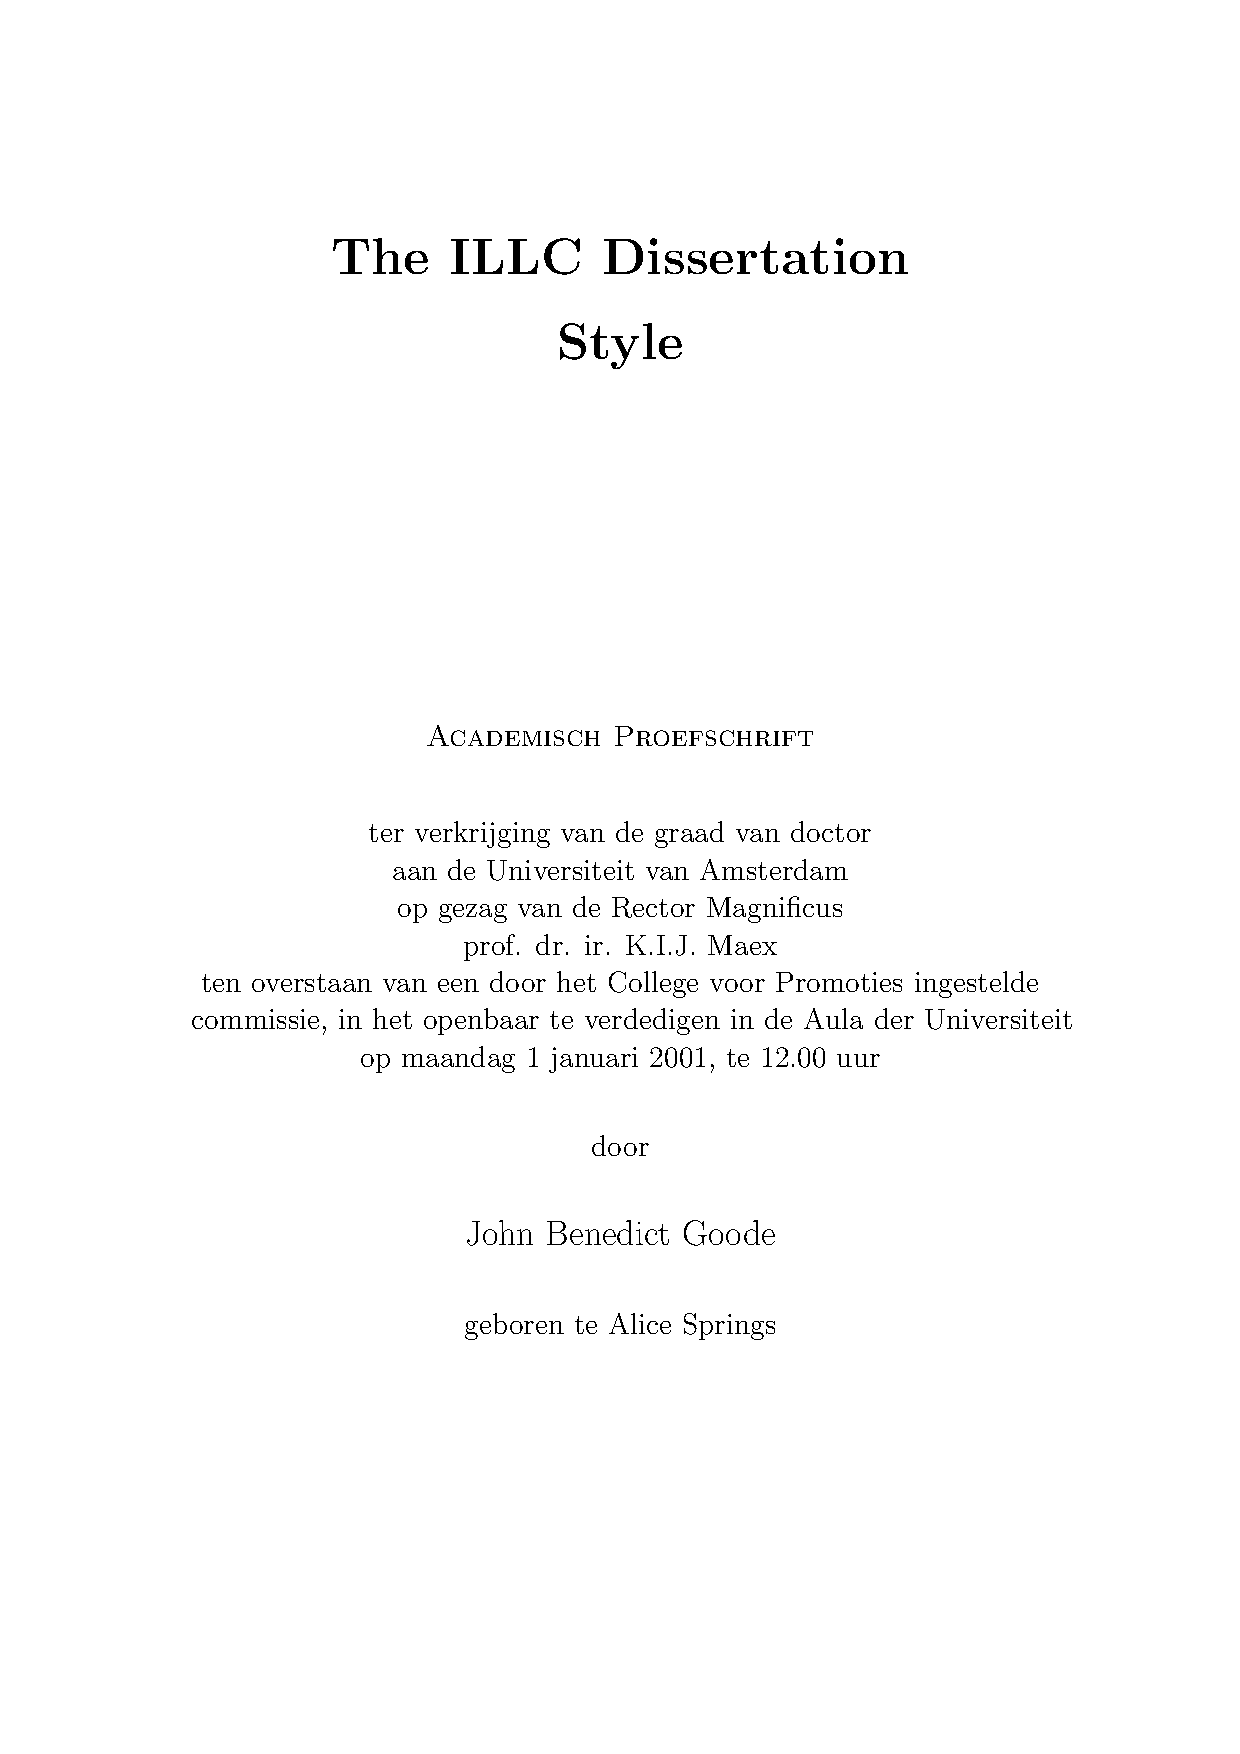
\includepdf[pages={1,2}]{titlepage_from_pedel.pdf}
%Formerly the pages were generated by the following content
 \par\vskip 2cm
 \begin{center}
 \printtitle
 \par\vspace {6cm}
 {\large \sc Academisch Proefschrift}
 \par\vspace {1cm}
 {\large ter verkrijging van de graad van doctor\\
 aan de Universiteit van Amsterdam\\
 op gezag van de Rector Magnificus\\
 prof. dr. ir. K.I.J. Maex\\                                 %PERSONALIZE
 ten overstaan van een door het College voor Promoties ingestelde\\
 \mbox{commissie, in het openbaar te verdedigen in de Aula der Universiteit}\\        %PERSONALIZE
 % Note: If your UvA PhD defense is located at the Agnietenkapel, simply write
 % 'te verdedigen in de Agnietenkapel \\', i.e. do not add 'der Universiteit'
 op maandag 1 januari 2001, te 12.00 uur \\ }        %PERSONALIZE
 \par\vspace {1cm} {\large door}
 \par \vspace {1cm} % Note: next should be your _full_ name
 {\Large Mostafa Mohajeri Parizi}                        %PERSONALIZE
 \par\vspace {1cm} % and your birthplace
 {\large geboren te Kerman} %PERSONALIZE
 % Note: NEVER include your country of birth, only the city of birth
 \end{center}
 \clearpage
 \noindent%
 {\bfseries Promotiecommissie}\\
 \\
 \begin{tabular}[t]{@{}llr}
 Promotor:      & Prof.dr.\ J.~Smith  & Universiteit van Amsterdam \\  %PERSONALIZE
 Co-promotor:   & Dr.\ T.~Jones       & Universiteit van Amsterdam \\  %PERSONALIZE
 \\
 Overige leden: & Prof. Dr. A. Aap    & Universiteit van Amsterdam \\  %PERSONALIZE
                & Prof. Dr. B. Benson & Universiteit van Amsterdam \\  %PERSONALIZE
                & Dr. C. Cornelissen  & Universiteit van Amsterdam \\  %PERSONALIZE
 \end{tabular}\\
 \\
 Faculteit der Natuurwetenschappen, Wiskunde en Informatica\\ %PERSONALIZE

\clearpage
} % Back to \pagestyle{plain}

%%%%%%%%%%%%%%%%%%%%%%%END of FRONT MATTER%%%%%%%%%%%%%%%%%%%%%%%%%%%

\thispagestyle{plain}
\mbox{}
\vspace{2in}
\begin{center}
{\em to me \\ \ \\
who did all the work on this}
\footnote{The dedication is optional}
\end{center}

\tableofcontents
\acknowledgments

I am very grateful to Prof.dr.\ J.\ Smith whose help proved really extremely
invaluable.\\[2ex]				
Alice Springs\hfill John B. Goode\\
October, 200X.



%%  now we can start with the real thing

\cleardoublepage
\pagestyle{headings}
\pagenumbering{arabic}

\chapter{Introduction}
\label{ch:intro}
Cyber-infrastructural systems are getting more integrated with our day-to-day life and have more impact on society, thus, there is a need for approaches to make sure that these systems are operating in a way that is more aligned with norms of society (or policies, rules, regulations). This means norms and policies should be considered as part of infrastructure development and maintenance cycles by the designers. On the other hand, infrastructures affect society and by extension, they are also affecting the norms and how that society is governed, so they should be already considered when policymakers and governance bodies are analyzing existing norms or implementing new policies and services. Taking modelling and model execution as a principal approach to analysing a system, intuitively, requires the experts to be able to create models of these concepts, which include executable models of the infrastructure, relevant norms, and, the social setting and its actors. The expressivity and flexibility required to encompass these aspects are not trivial. It is no longer just a model of infrastructure, social setting, and set of norms, but, it is an infrastructure that is utilized by social actors and governed by norms, a social setting that utilizes and monitors the infrastructure, and decides upon, modifies, analyzes and enforces the norms, and, norms that regulate the infrastructure and the social setting and have impacts on both.


The purpose of this thesis is to closely study the interactions between these concepts, and search for fundamental gaps in current methodologies utilized by system designers, policymakers, and governance bodies to find approaches for creating more expressive and tangible models that are also flexible enough for specifying different scenarios and use-cases in different domains. To propose realistic methods, aside from the theoretical analysis, proof-of-concept tools have also been developed or adopted at each step and are presented.


\paragraph{Social Norms and Behavioral Patterns}
A central theme in this thesis is norms and their relation with individual behavioral patterns. The definition of norms for specific use cases and domains is specified in corresponding chapters, but, it is valuable to set the tone on the complexities of this concept. The daily social life of a human is filled with objectively complex interactions, but somehow we can navigate these dynamic and nondeterministic interactions with a sufficiently low allocation of processing resources. A concept that aids us in doing so is norms, by defining what should and should not be the case and what is expected to happen or not to happen in certain contexts and under certain conditions, norms drive the actions in our fairly complex interactions. 


The fascinating thing about norms is that in any given situation, all parties involved are (somewhat) internally aware of the process and they can act accordingly. We can even deduce this (most probably) correct process in face of highly dynamic and nondeterministic situations with a multitude of variables. It seems like somehow we have converged very closely to a set of abstract, parameterized, context-based, and flexible scenario templates for interactions defined by norms that we use regularly as a coordination mechanism in society. These scenario templates have placeholders for different roles each with its own script, and most of the time we can (almost) precisely interpret a situation, select a relevant and applicable template and instantly fill the parameters and role placeholders with qualified values and infer some sort of decision tree that tells us how interactions can and should move forward. We even monitor and observe events and (own or others') actions and qualify them as traversal steps in these scenarios. Furthermore, concerning our part in a scenario, we seem to have internalized behavioral specifications or partial plans that allow us to enact and embody the role that we have filled with ourselves.


Interpreting the context, selecting a relevant and applicable scenario template, filling in the variables, and qualifying observation are the main components of utilizing scenario templates defined by norms. 

Take a simplistic example that is later on used in this thesis namely a sale transaction; regardless of the specific contexts, the norms for a typical sale transaction specify (almost globally accepted) predefined roles (buyer/seller), variables (item/price) and actions (offer/accept/pay/deliver) related to it. For an example of interpreting the context and selecting an applicable scenario take in-person shopping versus online shopping, while there are obvious differences in the variables and actions involved, we can think of them as the same thing that is a sale transaction with the same abstract template. For an example of filling in the variables, we can easily qualify actors and put them in proper roles the role of the seller in a sale transaction can be filled with ourselves, another person, a company, or more interestingly even an automated software in the form of a webshop. The same level of abstraction also applies to qualifying observations and expectations, receiving cash from an in-person buyer can be qualified as the same action as a notification of a transfer from a banking infrastructure, and the expectation of receiving an item in the next few moments from an in-person seller is the same as the expectations of receiving an oversea delivery in the next few weeks.

Scenario templates defined by norms are also highly dynamic and flexible. During an interaction, we are constantly monitoring the scenario for deviations from what we expect to occur. Some deviations can be negligible: while somewhat unexpected, they do not change the context of the interaction completely, like not receiving a delivery when it was supposed to arrive, or maybe there was a delay. However, some deviations completely change the context, like never receiving an item you paid for and not being able to contact the seller. What is interesting about deviations is that we even have modular and predefined contingency plans for when a concrete scenario is not played according to the expectations of its template. These plans can vary from attempting to fix the concrete scenario, like waiting a bit longer than expected for delivery, to revising some beliefs that resulted in the unexpected situation like removing a particular actor from the qualifications that make them suitable for the seller role to even rewriting the qualification or behavioral rules altogether like never buying anything from any unrecognized webshops.

\paragraph{Regulations, Compliance, and Governance}
Regulations are a form of norms that are (partially) concretized, written as a normative text, and enforced by some authoritative body that governs a system.  Cyber-infrastructural systems that affect members of society ideally should be fully compliant with the norms and regulations of that society. There are multiple ways to ensure compliance in a system, depending on its size, complexity, norms that govern it, and the governing bodies that are concerned with monitoring and regulating it. Some policies can be operationalized in terms of access control. For example, some infrastructures with pre-defined and static internal policies can be developed with the policies already hard-coded in them, intuitively, this is the most efficient approach whilst being the least scalable and maintainable. Some systems use run-time policy-making protocols like LDAP to make sure the infrastructure is running in a compliant manner by e.g., taking permission from policy enforcement points that take advice from policy decision points which in turn retrieve policies from policy information points. Then, by modifying the policies in information points, the administrators can control enforced policies without changing the infrastructure itself. 

These approaches can be referred to as \textit{compliant by design} and are arguably suitable for many situations. That is, until the point that norms in question become more complicated than simple non-conflicting, non-contradicting, easy-to-interpret regulative norms defined in terms of deontic notions of permissions, obligations, and prohibitions implemented in the form of ex-ante access rules. As is observed in the literature --and illustrated with multiple examples in this thesis -- norms do indeed become more complex much sooner than anticipated by most studies, and in fact, are vastly simplified in current compliance-checking approaches. 


Norms are more than a set of formal rules extracted from a legislative text: they emerge from multiple sources with different degrees of priority, and they require interpretation to be encoded and qualification to be applied within a social context. Furthermore, they continuously adapt, in both expression and application~\cite{Boella2014APractice}. Also, in any given context multiple normative sources may be concurrently relevant, and/or multiple interpretations of the same normative sources may be available (e.g. retrieved from previous cases), and these may be possibly conflicting. Finally, not all regulations are ex-ante norms about controlling actions prior to the performance of the action, instead, they are ex-post rules about what ought to be if certain actions have been performed already.% This makes conflict resolution and interpretation and concepts like consequences of actions detrimental parts of compliance-checking.


Furthermore, norms are traditionally distinguished between \textit{regulative} and \textit{constitutive} norms~\cite{Searle1969,Boella2004RegulativeSystems,Sileno2015}. Regulative norms regulate behaviors that exist independent of the norms and are generally prescribed in terms of \textit{permissions}, \textit{obligations} and, \textit{prohibitions} (e.g. traffic regulations). Constitutive norms determine that some entity (e.g. an object, a situation, a certain agent, a certain behaviour) ``counts as'' something else, creating a new institutional entity that does not exist independently of these norms. (for example, the concept of marriage or money as a legal means of payment). The concept of institutional power is particularly relevant in the context of constitutive norms, as it is used to ascribe institutional meaning to performances (e.g. raising a hand counts as a bid during an auction).

% A conceptual framework that instead contains both deontic and potestative dimensions is the one proposed by Hohfeld \cite{hohfeld1917fundamental}, whereas deontic logic, although much more popular, by definition focuses on regulative norms. %This work tries to take a step in the direction of taking these concepts into account in the process of designing compliant systems, or, modifying existing systems to be compliant.

These complexities in norms alongside the fact that cyber-infrastructural systems also include human actors and institutions that are certainly not fully compliant (and arguably, not even benevolent) means that such systems can not be fully compliant by design. Instead, such systems require \textit{governance}~\cite{vanengers2010egoverment}, which includes creation of new policies and regulations or modifying existing ones, enforcing these policies, providing supportive services, monitoring, analysing and imposing punishments and sanctions where needed. Intuitively, if components of the system can be feasibly compliant by design, that is a desirable attribute. However, when the governed system has rapidly changing technological components in it, there will be a need for approaches in adaptation of the governance that can keep up with these changes, and this thesis argues that modelling is a feasible approach. 


\paragraph{Models of Agency}
Agency is another concept that is central to this work. Software systems are generally considered to be void of real agency (specifically in legal terms) and are controlled through specific control structures, even if those structures consist of probabilistic flows that can change as the system interacts with its environment like in case of reinforcement learning they still have a control structure. This assumption becomes fuzzy when it comes to computational models of social actors as these models need to take agency into account, like executable models that should represent humans or organizations, as without access to fully developed artificial general intelligence, it is hard to claim that a software agent has agency. 

Then, the question is how do we model such actors? There are two main approaches used in the field to model concepts of agency such as objectives and preferences, namely these approaches are (1) modelling agents in terms of variables and mathematical functions, and, (2) modelling agents with means of agent-oriented programs often in the form of logic-based rational behavioral specifications, that often are deployed in a Multi-Agent System (MAS).


The first approach has many advantages, firstly, mathematical models are often more efficient in execution resulting in them being more scalable. Also, defining agents in terms of a few variables makes them easier for experimentation particularly in simulations, and, it also makes them much easier to manipulate at run-time, to simulate adaptation and learning processes. 

In general, when the purpose of a research is to study the outcome of social phenomena in certain settings without regards to the model of the input agent, mathematical models are suitable. An example of these approaches is the simulations of disaster response and relief, where purpose of the study is to find the optimal settings or infrastructures to minimize damage. In these cases the agents ---social or infrastructural--- are generally considered to have mathematical specifications that encompass a statistically realistic representation of how a civilian, a disaster response team, or an infrastructure will or should act in case of an incident or natural disaster as their utility function~\cite{arinta2019disaster,khouj2011disaster,chamola2021disaster}, keeping higher level concepts like purpose or intentions implicit in the models.


Where mathematical models fall short and programmable models are advantageous is studies where expressivity and transparency of the models is the main point. In these cases, even if the execution is less efficient and adaptability is harder to achieve, it is still worth to have self-explanatory and readable models of agents that have explicit notions of agency such as intentions and act in a configurable social setting. These are the cases where the purpose of the study is to analyze the agents and the society of agents without much regard to optimizing an outcome and often there is no obvious and well-defined utility function to optimize anyways. 


The study of norms and normative systems is one domain where these approaches are far more adopted, domains where analysing overall emergent behaviors, general trajectory of the society of agents, and the effect of norms and policies on that society are the main point of the study. Then the expressivity and transparency of the models and their decision-making becomes more important in analyzing and explaining (non-)compliant behaviors that goes beyond utility functions~\cite{van2019governmental}. 

This research intrinsically falls into this category, and, as it will be presented in later chapters, the Belief-Desire-Intention (BDI) model of agency \cite{Rao1995} is utilized in modelling agents. By specifying agents in terms of human-related attitudes, BDI agents are suitable in modelling social agents. More interestingly, majority of the concepts defined in the previous section about norms, like presence of behavioral specifications that can be matched and concretized in certain situations, or having contingency plans for failures are all already (partially) identified by BDI models to various degrees of success.


\section{Motivation and Research Questions}
%Prior to addressing how a complex data-sharing infrastructure and its participants can be modelled, we need to address why modelling such systems is important. 
The overarching motivation of this research has been in creation of a digital data market-places (DMP) specially in the field of logistics data. The need for data is exponentially increasing in all research and industries, and an environment like a DMP can provide different parties a place to share (or buy and sell) scientific or corporate data with each other. Although the presence of such environment can vastly improve the efficiency of data-oriented research and even prevent issues like data monopolies, there are certain risks involved, such as privacy issues, security issues, competitive corporate advantages, legal and ethical challenges, and, governance and accountability concerns.

Furthermore, as more governments (and other authoritative bodies) are implementing regulations to govern data transactions, such sharing environment needs to be compliant with these regulations, also actors in these markets like organizations and companies may have ad-hoc contractual agreements about data-sharing, and, they may also have internal policies like user agreements about how they can share data. The complexities of the market-places alongside the requirement for compliance results in a need for appropriate governance.

A crucial part of governance are policies. They provide a framework for decision-making, establishing guidelines and rules, and guiding the actions of individuals and organizations. Policies are generally about setting directions and goals for a system, regulating behavior, managing resources and risks, and, promote accountability. In the domain of data-sharing, policies have more specific roles.
%This work started by focusing on exactly that, how do we govern a data-sharing infrastructure and how can we create the policies for them? 

From the perspective of privacy, policies may specify how personal and sensitive data should be handled, defining the conditions for data anonymization and de-identification. Policies can also ensure compliance with relevant laws and regulations related to data protection, intellectual property, consent, and confidentiality. They define appropriate criteria for data access, such as applicable intentions and performance of appropriate actions, like obtaining consent. 

Policies can ensure fair and equitable data sharing, and establish rules for data usage, reuse, and retention~\cite{nissenbaum2004privacy}. They address ethical considerations such as fairness, transparency, and accountability in data-sharing practices. Policies may also be about data security, they establish measures to protect data from unauthorized access, breaches, and cyber threats. They outline security protocols, encryption standards, access controls, sufficient monitoring and data breach notification procedures. 

Another important aspect of policies and policy-making involves engaging relevant stakeholders, including individuals, industry representatives, researchers, and policymakers, to gather input, address concerns, and ensure that diverse perspectives are considered in shaping the data-sharing policies.


The importance of policies in data-sharing intuitively results in the crucial role of policy-making. In data-sharing, policy-making generally refers to the process of developing and implementing rules, guidelines, and frameworks that govern the collection, storage, access, use, and sharing of data and many other aspects of data-sharing. It involves the creation of policies, regulations, and standards that define the rights, duties and responsibilities, permissions, obligations, and power relations of various stakeholders involved in data-sharing, such as individuals, organizations, and governments. This lead to the main goal of this dissertation: \textit{Defining approaches, methodologies and tools for policy-making in the data-sharing domain}.

Policy-makers are required to take into account the effect and impact of their policies, for long-term and complex policy matters, this is only feasible with mathematical or computer-based models~\cite{Boulanger2005}. Modelling can play a crucial role in policy-making by providing insights, predictions, and evaluations that inform the development, implementation, and assessment of policies. Modelling helps with understanding complex systems allowing policymakers to gain a better understanding of systems and their dynamics. Modelling enables scenario analysis by simulating different scenarios and predict the potential outcomes of policy choices resulting in more optimized policies with more balanced between goals. Finally, models can facilitate more transparency and better policy communication with stakeholders and even system designers.

There are different types of modelling used in the different communities to assist in policy-making. These approaches vastly differ in their focus, methodology, and, modelling time-frame. From macroeconomics to system dynamics to agent-based modelling, each approach has its own use-cases in specific domains, and there are arguments to use one or a combination of these approaches in different use cases~\cite{Scholl2001,silverman2023,dosi2019,Dignum2008}. Agent-based models are specially suitable for policy-making as they define the behavior of individuals to build emergent trajectory of the system as a whole. In a real system, where policies are based on top-down assumptions of behavior, many changes occur bottom-up from individual actors' actions~\cite{Dignum2008}. This dissertation focuses on utilizing agent-based models for policy-making; then, the more concrete goal of this research would be: \textit{Defining approaches, methodologies and tools for policy-making in the data-sharing domain based on Agent-Based Modelling}.



While this dissertation focuses on data-sharing, it is not only data-sharing use-cases that are in need of such methods for policy-making and system design. More aspects of our day-to-day life are being \textit{controlled} by automated processes; visa applications, job applications, credit placements, mortgage and insurance are just a few examples and one can only imagine that the list will continue to grow as time goes on. Even if data-sharing regulations are a relatively new phenomena, when taken in a broader sense, there are already regulations implemented for other domains that are now becoming more automated, and when the decisions are made in an automated manner, then the goal will expand to defining policies for any cyber-infrastructural system with respect to arbitrary (regulative and constitutive). This dissertation takes the aforementioned goals, by assuming (agent-based) modelling and model execution as a principal step in system design and policy-making:

\begin{displayquote}
\textbf{Main Research Question:} \textit{How can we model a norm-governed cyber-infrastructure for the purpose of policy-making?}
\end{displayquote}


\section{Approach and Scope of this Thesis}
The first step in defining the scope of this work is to break the main research question structurally by further defining what needs to be modelled: a norm-governed cyber-infrastructural system. The main components are norms, social setting and software/infrastructure that create the system as a whole. We also need to define what are the requirements of these models to be suitable for policy-making.
%but also there is the assumption of openness, which means the system that is being modelled interacts with, affects and get affected by an external undefined environment. 
Then, the main research sub-questions should intuitively become how to model each of these three components. But, unfortunately it is not that simple as these concepts are not at the same level of abstraction for the purposes of this research. 
%Starting from the concept of social setting, it is arguably the main focus of this work, modelling social agents seems to be one of the keys to modelling such systems, but why? 

Take the concept of norms, while modelling them is essential for the whole picture, it is still social agents that act as the governance bodies that regulate other entities of the system, and in effect, it is social agents that are being governed, i.e., it is very hard to talk about norm-related concepts (e.g. sanction) without referring to human-related concepts (e.g. intention). Indeed it is rare to see an infrastructure being punished for non-compliant actions without referring to a social agent (a person, company, institution, organization) as the main liable entity for those actions, or, it would be untenable to say a piece of software or infrastructure is imposing a sanction without the presence of a social agent (an organization, consortium, government)  holding the power to impose that punishment. In effect, norms as are studied in this research ---as it is often the case in real life--- do not have isolated meaning by themselves and without the social setting. The same logic goes for software and infrastructural components, while being another important part of the system model, it is still their usage by and effects on social agents that is being scrutinized.
%Furthermore, while software modelling is a mature and advanced field of study, the purposes of this work are aimed at possibility of a more realistic view of software systems. Such realistic view reveals that software and infrastructural systems are very technology-dependant subjects and high-level models of them are rarely complete without their low-level technological details. It is hard to discuss about a data transfer without mentioning if that data is personal or not, anonymized or not, plain or encrypted, or if the transmission channel is secure or not. 

In summary, in the context of this thesis, social agents are the glue that hold the models together and they have the following requirements for them to be suitable in policy-making: (1) As the central part the models, the agent models should be expressive, readable, and, transparent for the whole system model to also posses these qualities; (2) The agent models need to incorporate norm reasoning for the system as whole to be insightful about norms and policies; (3) The agent models should have interoperability with software (models) to allow the framework to model socio-technical systems; (4) The framework should satisfy usability requirements, this encompasses multiple qualities such as modularity, scalability, testability, and, maintainability of the models.

\begin{displayquote}
\textbf{Research Question 1:} \textit{How to create expressive and modular models of social agents?}
\end{displayquote}


%The short answer to this question is that agent-based programming is the most suitable approach to create models of agents. The alternate approach that is mathematical models while having many advantages are simply not transparent enough at the required level of abstraction for our use-cases: it is not easy to model intention for example in an effectively optimizer agent that has a utility function driving its decisions. 


The approach adopted in this work to agent-based programming is the the Belief-Desire-Intention model. While there are multiple BDI frameworks introduced in the literature, after much deliberation and testing it turned out they did not meet the requirements of this study, maybe the most important one being modularity.

In the process of this work, a BDI (and MAS) framework called AgentScript Cross-Compiler (ASC2) was designed and developed with these requirements in mind which uses a programming language based on the AgentSpeak(L). As the main requirement, modularity is addressed in the sense that ASC2 does not assume a hard-coded reasoning and decision-making cycle for agents, an in fact almost every aspect of the agents is programmable. This is made possible mainly because of two reasons. 

Firstly ASC2 utilizes actor-oriented programming via Akka actor framework meaning each agent consists of multiple actors each with their own role that can communicate through internal messaging, effectively making an agent a modular actor micro-system in itself. Secondly, by following software engineering best practices and methodologies like Dependency Injection and Inversion of Control. By using Dependency Injection, most components and sub-components of an an agent can be sent to it as potentially customized dependencies. Furthermore, with Inversion of Control it is the lower level components that are mainly controlling the nuanced execution cycle when higher level components only define abstract control flows. The ASC2 framework is introduced from an engineering perspective in Chapter \ref{ch:asc2}. 

Next, there is the issue of how to model software and infrastructural entities. This question effectively falls out of the scope of this thesis as there is an extensive body of research on software modelling, instead, the focus is on their utilization by social agents. Important steps are taken to provide a high level of interoperability for social agents modelled in ASC2 to virtually any type of model of software and infrastructural entities that are being used by the designer and policy-maker, including the actual real entities.

\begin{displayquote}
\textbf{Research Question 2:} \textit{How can social agents utilize software and infrastructural models or entities?}
\end{displayquote}

The answer to this question is in the \textit{Cross-Compiler} part of ASC2. As it is addressed in Chapters~\ref{ch:devops} and~\ref{ch:normative_advisors}, after compilation ASC2 agents are technically JVM programs meaning they are indeed interoperable with any system that for example a Java program can utilize or communicate with. This results in much more effective modelling cycles as there is far less concern about connecting the models to real system or interfaces.


Next is the notion of norms, modelling them including social norms, regulations, contractual agreements, internal policies is an important part of the modelling that this thesis aims at. However, while different approaches and ideas about modelling norms are explored in this work, defining any novel approach to do so falls out of the scope of this thesis for both theoretical and practical reasons. The practical reason is mainly that other threads of dedicated research were being performed on this matter within the research group that both affected and utilized this work. The theoretical reason is that there are various levels of abstraction that norms can be modelled for different use-cases and this work stays agnostic to which approach is the most suitable. However, the question that is studied is the concept of norms from the perspective of social agents:

\begin{displayquote}
\textbf{Research Question 3:} \textit{How can social agents reason with and about norms?}
\end{displayquote}

The main concern of this thesis on this question has been to study the interactions between social agents and norms, including the interpretation and qualification of events between institutional and physical realities, understanding compliant and non-compliant behaviors and the relation between compliance and autonomy. This is addressed in section \ref{ch:eumas} with introducing the concept of normative advisors, a flexible approach that can be utilized by social agents to have an understanding of normative positions in their environment without reducing their autonomy.


This thesis started from the assumption that agent-based programming is a more expressive approach than mathematical models with utility functions. However, it also revisits the validity of that assumption. BDI models --- and more specific to this work, AgentSpeak(L)-like models--- are designed with expressivity and readability as a first class requirements, but these are still not fully solved issues. Mathematical models of agents are mainly aimed at optimizing a certain utility function, it can be conceptually viewed as if such an agent has the quantitative objectives, desire or preference of maximizing that function. Then, what are the objectives, desires or preferences of an agent-based program? Furthermore, in the process of this research it was observed that by adding norms and normative reasoning into the agents, these concepts become even more important. Norms in every form can be  conflicting and such conflicts can rarely be resolved by quantitative approaches, then, how should an agent program behave in face of conflicts? There is not clear cut answer to this question as it will depend on the context, and this thesis only addresses this by taking the stance that:  it depends on the preferences and desires of the agent, however, the designer should be able to program these notions. The issue addressed here is not about what is the \textit{most appropriate} behavior of the agent as the consequence of its decision-making and conflict resolution; that will depend on what the designer is modelling. Instead, it is how such decision-making can be expressed in a transparent manner:

\begin{displayquote}
\textbf{Research Question 4:} \textit{How can we model desires and preferences of agents?}
\end{displayquote}

This question is addressed in Chapter \ref{ch:aamas} by introducing the concept of explicit preferences in the form of CP-Nets into the BDI model and the AgentScript programming language. With this approach, the designer can separate the concern between the procedural or the \textit{how-to} knowledge of the agent program from the preferential or \textit{what-to} knowledge. This makes the decision-making of the agents more transparent which is a requirement in models that are created for the purpose of analysis. 

The last issue addressed in this thesis is the practicality of utilizing agent-based models as part of real-world system design and policy-making, not only as they are used in this work but the whole agent-based modelling community. It is always the case that accessibility and usability of the tools in a certain methodology is an important part of their adoption, it is hard and mostly not feasible to convince domain experts like programmers to utilize an approach if they need to also learn a whole new set of tools and ecosystems. This is also the case for utilizing agent-based models and has been a major concern in this work

\begin{displayquote}
\textbf{Research Question 5:} \textit{How to make agent-based modelling a usable approach for mainstream designers?}
\end{displayquote}

In the recent years the tools created for design and development in mainstream software community are becoming more advanced and efficient. A few examples of such tools are IDEs, testing libraries, build tools, code coverage tools, code repositories, and, DevOps system like CI/CD tools. Intuitively it is advantageous to allow for utilization of these tools in agent-based modelling and model execution. As a side effect of its design, ASC2 programs can directly utilize any system or library available to JVM-based programs without the need for any extra interfacing as after compilation, ASC2 programs become JVM-based programs. This includes all the development tools listed above and many others. In Chapter \ref{ch:emas} it is shown how utilizing these tools, not only benefits agent and multi-agent system (MAS) communities in e.g., testing their designs with mainstream automated testing tools, but more importantly, allows agent models to be used as part any software development process, be it for testing or any other purpose.


\section{Research Context and Collaborations}
Before starting the next chapter, I will try to put this dissertation into the context and environment that the research was conducted, highlighting the parallel research that had a connection to it and some of the events that affected it. The research was done in the Complex Cyber-Infrastructures (CCI)\footnote{\url{https://cci-research.nl/}} research group and was funded by the project Data Logistics for Logistics Data (DL4LD)\footnote{\url{https://dl4ld.nl/}}. There were two other closely related projects: Secure Scalable Policy-enforced Distributed Data Processing (SSPDDP)\footnote{\url{https://cr-marcstevens.gitlab.io/sspddp/}} and Enabling Personalized Interventions (EPI)\footnote{\url{https://enablingpersonalizedinterventions.nl/}} that shared research with DL4LD.

Following highlights some of the parallel research threads that were conducted mostly by other PhD candidates and post-doctoral researchers alongside this work. In the context of this issertation, Agent-Oriented Programming approaches were utilized for developing Agent-Based Models. The counterpart to this are the mathematical models of agents which were simultaneously studied in the context of the group by Fractic et. al. \cite{Peter}. Where this thesis tries to find approaches in enhancing models for developing policies, there were parallel works that focused on what these policies should be, including risk management and enforcement schemes by Zhou et. al. \cite{Xin}. Another thread of research, as it was mentioned in the introduction was about norm reasoning. The results of these works done by Thomas, Lu-Chi, Milen \cite{Thomas,Milen,Lu-Chi}, are used throughout future chapters . Finally there was a more network-focused side of this work, mainly on development of Data Market-Places e.g., Reggie et. al. \cite{Reggie}, Lu et. al. \cite{Lu}.

Finally, majority of the time dedicated to this research overlapped with COVID-19 restrictions, and apart from ``normal'' issues, it meant there was little to no real interaction with the industry partners that were the initial stakeholders of this project. To provide full transparency for the reader the phrase ``it turned out that it is not only data-sharing use-cases that are in need of such methods for policy-making and system design'' in the motivation section, while still true, also partially means that it is considerably more challenging to study policies and policy-making in data-sharing without the presence of stakeholders that have access to data and are interested in sharing them.  As a result, while this research was at a relatively high level of abstraction at its inception, for better or worse, became even more theoretical that it was intended to be ---or I intended it to be---, but fortunately, my supervisors were already interested in the more theoretical side of the issue \cite{Tom,Giovanni} which greatly guided this research in every aspect. However, by interacting with the respective communities e.g., AI and Law, Normative Systems, and, Multi-Agent Systems, my observation was that there is an interest for more practical and usable approaches to bring the long standing results of these communities closer to mainstream domains. For this reason, every chapter of this dissertation includes development of tools or proof of concepts that utilize fairly mainstream software ecosystems.  

\section{Structure of the Dissertation}







\chapter{Developing a Suitable MAS Framework: ASC2}
Agent-based modelling is a valuable tool in designing complex socio-technical systems. The chapter introduces an Agent-Oriented Programming (AOP) framework based on the Belief-Desire-Intention (BDI) model of agency. There are multiple BDI frameworks already introduced in the literature. Prior to development of ASC2, we tried to adapt and utilize multiple of these frameworks, while there were different advantages and disadvantages to each of them, in the end, the main reason that resulted in designing and developing yet another framework was firstly interoperability and and secondly maintainability. None of these framework allowed for seamless interoperability between agents and other mainstream software. Also, these frameworks had most of the agent's reasoning hard-coded into them which is detrimental to experimentation on alternate theories of an agents behavior. By getting inspirations from the design of previous works, the novelty of this framework is in relying on the Actor model, instantiating each intentional agent as an autonomous micro-system run by actors. The hypothesis behind this choice is that defining the agents via actors results in a more fine-grained modular architecture that is more modifiable and that the execution of agent-oriented programs is enhanced (in scalability as well as in performance) by relying on robust implementations of Actor models such as \textit{Akka}.


\section{Introduction}
Agent-based models have an intuitive mapping to behavioural descriptions, and for this reason are extensively used for modeling and simulations of social systems. However, \textit{agent-based programming} is not only relevant for simulation. Complex Cyber-Infrastructures like those used for data-sharing as digital marketplaces exhibit the double status of computational and social systems; regulating these infrastructures requires reproducing to a certain extent constructs similar to those observed in human reasoning (e.g. For which purpose is the agent asking access to the resource? On which basis is the infrastructure granting access?). For \textit{traceability} and \textit{explainability} reasons, decisions concerning actions need to be processed by the infrastructure as much as relevant operational aspects. Agent-based programming, by looking at computational agents as intentional agents, provides this level of abstraction available \textit{by design}. However, this raises concerns on how we can efficiently map logic-oriented agent-based programs into an operational setting, a problem motivating the present research.


% ASC2 is a higher-level logic-based DSL for specifying scripts for intentional agents, i.e. sets of behavioural responses to environment conditions that are expected to achieve certain purposes. The standard approach to these type of languages is to use them by means of an interpreter. This work reports on a experiment to approach the via a trans-compilation tool, i.e. translating such higher-level DSL to a lower-level executable language (in this case Scala) that can be then compiled and executed.


This chapter introduces ASC2, a logic-based AOP framework in which agents are modular micro-systems run by actors. To evaluate the feasibility of this approach for future developments, a first implementation of ASC2 based on Akka runnig on JVM is compared with three other relevant AOP frameworks (Jason \cite{Bordini2005}, ASTRA \cite{Astra} and Sarl \cite{Astra}) by means of 3 benchmarks (token ring, chameneos redux and service point), known to capture relevant patterns in concurrent applications. This performance evaluation shows that despite its relative youth and the new implementation approach, ASC2 is competitive against existing frameworks, making it worthy of further investigation.
% The initial performance evaluation shows that despite its relative youth and new implementation approach, ASC2 is competitive against existing frameworks, making it worthy of further investigation.

The chapter proceeds as follows: Section~\ref{sec:agere:background} provides some background on relevant concepts and related works. Section~\ref{sec:agere:method} presents the ASC2 framework. Section~\ref{sec:agere:evaluation} reports on the empirical experiments comparing ASC2 with other frameworks. Section~\ref{sec:agere:discuss} compares the frameworks qualitatively. A note of future developments ends the chapter.


\section{Background}
\label{sec:agere:background}
\subsection{Agent Oriented Programming}

Agent-Oriented Programming (AOP) is a programming paradigm that uses mental attitudes to model autonomous computational agents. Introduced in 1993 by Shoham \cite{shoham1993agent}, it has attracted increasing attention ever since and is believed to provide an effective abstraction to approach complex software systems (e.g. \cite{Sarl}). In the beginning it was presented as a specific version of Object Oriented Programming (OOP): whereas object classes contain arbitrary components, agent types share the same types of mental states and of structural relationships/mechanisms involving those states. 


\subsection{Belief-Desire-Intention (BDI) Model}
% Having its roots in a theory of mind \cite{bratman1987intention}, and so referring to categories that are used typically to address human behaviour to describe agents, the \textit{belief-desire-intention} (BDI) model \cite{Rao1995} has been extensively investigated as basis to represent computational agents that exhibit rational behaviour \cite{Herzig2017}. 
% % uses taxonomies that are used typically to address human behaviour to describe agents.
% \textit{Beliefs} are the factual (and possibly inferential) information the agent has about itself or its environment. \textit{Desires}, in their simplest form, are objectives the agent wants to accomplish. % \Gio{(i.e. facts desired to be true)}.
% %in the environment. 
% \textit{Intentions} are the courses of action the agent has committed to. In practice, BDI agents include concepts of \textit{Goals} and \textit{Plan}. Goals are instantiated desires % associated to reactive behaviors to certain events 
% and plans are abstract specifications relating a goal to the means of achieving that goal (intentions become commitment towards plans). Multiple programming languages and frameworks have been introduced based on the BDI model, as AgentSpeak(L)/Jason \cite{RaoAS1996,Bordini2005}, 3APL/2APL \cite{Dastani2APL}, GOAL \cite{Hindriks2009a} and IMPACT \cite{IMPACT}.

BDI frameworks are usually described in terms of an \textit{agent theory} and  an \textit{agent computational architecture} \cite{Fisher2007}. % The latter could further divided in data structure and execution cycle. 
The agent theory usually refer to Bratman's theory of practical reasoning \cite{bratman1987intention}, describing the agent's cognitive state and reasoning process in terms of its \textit{beliefs}, \textit{desires} and \textit{intentions}. Beliefs are the facts that the agents believes to be true in the environment. Desires capture the motivational dimension of the agent, typically in the more concrete form of \textit{goals}, representing procedure/states that the agent wants to perform/achieve. Intentions are selected conducts (or \textit{plans}) that the agent commits to (in order to advance its desires). The agent architecture varies depending on the platform. Taking for instance the BDI platform Jason \cite{Bordini2005}, it consists of perception and actuation modules, a \textit{belief base}, \textit{intention stacks} and an \textit{event queue}. The BDI execution model, describing the agent's reasoning cycle, can be summarized as follows:
\begin{enumerate}
	\item  observe the external world to update the internal state (perception);
	\item  update the event queue with percepts and exogenous events;
	\item  select events from the event queue to commit to;
	\item  select plans from the plan library that are relevant to the selected event;
	\item select an intended means amongst the applicable plans for instantiation; %(intended means)
	\item push the intended means to an existing or a new intention stack; %(plan instantiation)
	\item select an intention stack and pull an intention, execute the next step of it; % (intention selection)
	\item if the step is about a primitive action, perform it, if about a sub-goal post it to the event queue.
\end{enumerate}
As exemplified by this description, an essential feature of BDI architectures \cite{Rao1995} is the ability to instantiate plans that can: (a) react to specific situations, and (b) be invoked based on their purpose. Consequently, the BDI execution model naturally relies on a \textit{reactive} model of computation (cf. \textit{event-based programming}, typically used for user interfaces). % In effect, all BDI programming languages presents some form of reactive rules, except for GOAL that does not include the typical goal-driven reasoning as goals are modelled as part of the agent's belief set. 
Multiple programming languages and frameworks have been introduced based on the BDI model, as AgentSpeak(L)/Jason \cite{RaoAS1996,Bordini2005}, 3APL/2APL \cite{Dastani2APL}, GOAL \cite{Hindriks2009a} and IMPACT \cite{IMPACT}.

% \subsubsection{Goal-plan rules}
% As a general definition of reactive rules for BDI execution models we consider the notion of \textit{goal-plan rules}, i.e. an \textit{uninstantiated specification of the means for achieving a goal} \cite{Rao1995}, capturing the procedural (\textit{how-to}) knowledge of the agent. % When a goal-plan rule is applicable, it is an optional course of action available to the agent. 
% A goal-plan rule $pr$ is a tuple $\langle e, c, p \rangle$, where:
% \begin{itemize}
% 	\item  $e$ is the \textit{invocation} condition, i.e. the event that makes the rule \textit{relevant}; 
% 	\item  $c$, the \textit{context} condition, is a first-order formula over the agent's belief base, which makes the rule \textit{applicable};
% 	\item  $p$, the \textit{plan} body, consisting of a finite and possibly empty sequence of steps $[a_1,a_2,...,a_n]$.% where each $a_i$ is either a \textit{goal} (an invocation attempting to trigger a goal-plan rule), or a \textit{primitive action}. 
% \end{itemize}
% A goal-plan rule $pr_i$ is an option or a possibility for achieving a goal-event $e$, if the invocation condition of $pr_i$ matches with $e$, and the preconditions $pr_i$ matches the current state of the world, as perceived or encoded in the agent's beliefs. 
% In BDI implementations, the preference between these optional conducts is specified through static rankings assigned by the designer, typically via the ordering of the rules in the code. 



\subsection{Actor Model}
The Actor model, introduced in \cite{Hewitt}, is a mathematical theory that treats \textit{actors} as the primitives of computation \cite{hewitt2010actor}. Actors are essentially reactive concurrent entities. % that use message passing as the basis of their communication. 
When an actor receives a message it can %concurrently 
send messages to other actors; \textit{spawn} new actors; modify its reactive behavior for the next message it receives.
Originally proposed as a tool for the theoretical understanding of concurrency, the Actor model serves now as the basis of several production-level solutions for distributed and asynchronous systems, and for reactive programming. These solutions include: Akka \cite{AKKA}, a library developed for the JVM environment, enriched by a strong community with multiple complementary tools for distributed environments and stream processing; the C++ Actor Framework (CAF) \cite{CAF}, a library %written in C++ 
for creating concurrent programs in C++; Pony \cite{PONY1,PONY2}, an actor language for building robust parallel systems by providing data-race free isolation for actors. A comprehensive overview and benchmark over these works can be found in \cite{RunActor}. 


\subsection{Related Work}
Multiple AOP and BDI frameworks have been introduced proposing diverse approaches towards language, execution model, reasoning process, etc. Jason \cite{Bordini2005} is plausibly the most known (e.g. it is the most used choice in the Multi-Agent Programming Contest \cite{mapc}), and has been constantly developed in the last 15 years. It is implemented in Java and is essentially an \textit{interpreter} for a logic-based DSL, namely an extended version of AgentSpeak(L) \cite{RaoAS1996}.  Two recent frameworks inspired by Jason are Pyson \cite{pyson} and LightJason \cite{LJ}. Pyson is an interpreter implemented in Python and uses \verb+MapReduce+ technology as execution infrastructure in order to achieve better scalability specifically w.r.t. the number of agents. LightJason is a BDI framework based upon a variation of AgentSpeak(L) and whose interpreter aims to improve the scalability of Jason by implementing a concurrent platform following best practices in software engineering.

ASTRA \cite{Astra} is yet another framework inspired by AgentSpeak(L)/Jason and is also implemented in Java, but, unlike Jason, it is not an interpreter. ASTRA relies on a \textit{compilation} approach: through a build pipeline the DSL is first translated to pure Java code and then the Java code is compiled to byte-code for execution. In contrast, the Sarl \cite{Sarl} framework has not been introduced as a BDI platform and then it does not use the same abstractions. Nonetheless it is an AOP framework written in Java that also uses compilation, and for these reasons it is relevant for the current study.

% and that puts scalability amongst the requirements it aims to satisfy. 

Although several AOP/BDI frameworks have been introduced in the recent years (all hinting to problems of scalability), there is a small amount of empirical data available about how they perform in comparison to each other. The most notable exception is  \cite{Cardoso2013}, in which multiple actor and agent frameworks (2APL \cite{Dastani2APL}, GOAL \cite{Hindriks2009a}, Jason and Akka) are benchmarked. Their results showed that Jason outperformed other BDI frameworks by far and scaled almost on par with Akka. However, at that time (2013), none of these newer frameworks had been introduced yet, and Akka had not the support it has today. Strangely enough, none of these new AOP frameworks has the Actor model at their foundation. The present chapter aims to investigates part of this gap.


\section{AgentScript Cross-Compiler (ASC2)}
% In this section the ASC2 framework is introduced. 
% At its core 
This section introduces ASC2, however, as this framework is central to this thesis, detailed descriptions of different parts related to specific concepts is presented in the respective sections. The ASC2 framework consists of: (a) a logic-based Agent-Oriented Programming DSL; (b) an abstract agent run-time architecture; (c) a translation method that generates executable models from models specified by the DSL; (d) tools that support the execution of models. We provide here a brief overview on these components.

\subsection{ASC2 DSL}
\label{section_dsl}

The ASC2 DSL has a very close syntax to AgentSpeak(L) language and includes some of the extensions provided by Jason. The main components of the DSL are (1) initial beliefs, (2) initial goals, and (3) plan rules. Initial beliefs are a set of Prolog-like facts and inferential rules that are potentially non-grounded declarative rules (Prolog-like), used to infer beliefs from beliefs. Initial goals designate the first intentions to which the agent commits. These can be used as a way to initialize an agent in their environment, and maybe start interacting with other agents. 

Plan rules are potentially non-grounded reactive rules in the form $e : C \Rightarrow H$ that map different internal or external events $e$ (e.g, \textit{goal adoption}, \textit{belief-update}) to a sequence of executable steps $H$ called the \textit{plan body} which the agent will perform in response to the event. The steps of a plan body can include belief query, belief update, sub-goal adoption, primitive actions, variable assignment, and control flow structures (loops and conditionals). Each plan also has a context condition $C$ which is a Prolog-like expression that represents when that plan is applicable. The full grammar definition of ASC2's DSL is presented in Listing~\ref{listings:asc2grammar}.

\begin{listing} 
\begin{minted}[escapeinside=00,mathescape=true]{js}
agent           0$\rightarrow$0 beliefs initial_goals plans
beliefs         0$\rightarrow$0 (term '.')*
initial_goals   0$\rightarrow$0 ('!' atomic_formula '.')*
plans           0$\rightarrow$0 (plan '.')*
plan            0$\rightarrow$0 ( '@' atomic_formula )*
                trigger_event ( ':' context )
                '=>' body_definition '.'
trigger_event   0$\rightarrow$0 ( '+'|'-'|'+!'|'-!'|'+?' ) atomic_formula
context         0$\rightarrow$0 term
body_definition 0$\rightarrow$0 body_formula ( ';' body_formula )*
body_formula    0$\rightarrow$0 ( '!'|'+'|'-' ) literal
                |  loop
                |  conditional
                |  primitive_call
                |  <VARIABLE> '=' term
term            0$\rightarrow$0 <VARIABLE>
                |  '(' term ')'
                |  <INTEGER> | <FLOAT> | <STRING> | 'true' | 'false' 
                |  <ATOM> '(' term_list ')'
                |  term operator term
                |  'not' term
                |  '[' term_list ( '|' term )? ']'
                |  <ATOM>
                |  primitive_call
atomic_formula  0$\rightarrow$0 <ATOM>
                |  <ATOM> '(' term_list ')'
literal         0$\rightarrow$0 <VARIABLE> 
                |  atomic_formula               
term_list       0$\rightarrow$0 term ( ',' term )*
operator        0$\rightarrow$0 '**'|'*'|'/'|'mod'|'+'|'-'|'='
                |'=='|'!=='|'!='|'<'|'<='|'>'|'>='|'is'|'>>'
                |'^'|'&&'|'||'|':-'
primitive_call  0$\rightarrow$0 '#' <ATOM> ( '.' <ATOM> )* '(' term_list? ')'
loop            0$\rightarrow$0 'for' '(' <VARIABLE> 'in' term ')' 
                '{' body_definition '}'
conditional     0$\rightarrow$0 'if' '(' term ')' '{' body_definition '}'
                ('else' 'if' '(' term ')' '{' body_definition '}')*
                ('else' '{' body_definition '}')?
\end{minted}
\caption{AgentScript's DSL grammar defenition}
\label{listings:asc2grammar}
\end{listing}%\label{listings:asc2grammar}


An example of an ASC2 DSL that shows part of the script for a domestic robot is presented in Listing~\ref{lst:domestic_robot}, where lines 2-4 are initial beliefs, line 6 is an inferential rule, line 9 is an initial goal and lines 12-15 define an example plan. This script is further expanded on in the next chapter.

\begin{listing}[!h]
\begin{minted}[fontsize=\small,linenos]{prolog}
% initial beliefs and inferential rules
main(fish). soup(veg). wine(white).
restaurant(french).
at(home).

meal(S,M,W) :- soup(S), main(M), wine(W).

% initial goals
!go_order(french,meal(veg,meat,white)).

% plans
% P1
+!go_order(Loc,Meal) :
        restaurant(Loc) && not at(Loc) =>
        #move_to(Loc);
        !order(Meal).
...
\end{minted}
\caption{An example script of ASC2 DSL}
\label{lst:domestic_robot}
\end{listing}

%  An example of initial goals for the domestic robot agent can be:
% \begin{minted}[fontsize=\small]{prolog}

% \end{minted}

%  An example of a plan in the domestic robot agent that tells it to go a location and order a meal:
% \begin{minted}[fontsize=\small]{prolog}
% +!go_order(Loc,Meal) :
%     restaurant(Loc) && not at(Loc) =>
%         #move_to(Loc);
%         !order(Meal).
% \end{minted}

% Note that this plan is applicable only if the location is believed by the agent to be a restaurant, and, the agent believes it is currently not at that location. The plan body has two steps, one is a primitive action \asc{#move_to(Loc)} which is a low level call to a function and the second one is adoption of a sub-goal \asc{!order(Meal)}.

%When a plan body $f$ is matched with an event $e$, it is said that $f$ is \textit{relevant} for $e$. Each plan also has a context condition $c$ which is a Prolog-like expression. When a plan $f$ is relevant for $e$ and also $c$ holds, it is said that the $f$ is \textit{applicable} for $c$.  The grammar definition of ASC2's DSL is presented in Listing~\ref{listings:asc2grammar}. % \textcolor{red}{how much more does this section need to expand?}




\subsection{ASC2 Run-time Architecture}
\label{section_arch}
ASC2 is primarily motivated by AgentSpeak(L)/Jason as a starting point, and in its default setting it is designed to have the (almost) the same functional architecture. However, from a structural perspective, ASC2 is novel in the sense that it utilizes actor model to instantiate agents as actor micro-system. Because of this, the run-time architecture of ASC2 agents can and should be inspected from both functional and structural perspectives. 

\subsubsection{ASC2 Functional Architecture}
From a functional perspective, ASC2 agents (by default) conceptually follow a reasoning flow very close to the reasoning cycle defined by AgentSpeak(L)/Jason. An ASC2 agent consists of a set of beliefs $B$ called belief base, a set of plans $P$ called plan library, a set of events $E$, a set of intentions $I$, and three selection functions: $S_E$,$S_O$,$S_I$. When the agent receives an (internal or external) event or adopts a goal, it is added to $E$. The selection function $S_E$ selects an event to process from $E$.
%. 

% \begin{definition}
% [Plan] A (reactive) plan is specified by $e : C \Rightarrow H$ where $e$ is a triggering event, $C$ is a formula capturing context conditions, and $H$ is a sequence of sub-goals or actions to be performed at the occurrence of the trigger event.
% \end{definition}

Then, this event is matched with the triggering events in the heads of the plans in $P$. The plans that their triggering event unifies with this event are called \textit{relevant plans} and their unifier is called the \textit{relevant unifier}. Then for each relevant plan, the relevant unifier is applied to the context condition of that plan, and by querying against $B$ a substitution is created such that the context is a logical consequence of $B$. The composition of relevant unifier with this substitution is called an \textit{applicable unifier}. 

% \begin{definition}
% [Relevant plan] A plan in the form of $e : C \Rightarrow H$ is a \textit{relevant plan} with respect to an event $\epsilon$ iff there exists a most general unifier $\sigma$ such that $\epsilon\sigma = e\sigma$. Then, $\sigma$ is referred to as the relevant unifier for $\epsilon$.
% \end{definition}

% \begin{definition}
% [Applicable plan] A plan in the form of $e : C \Rightarrow H$ is an \textit{applicable plan} with respect to an event $\epsilon$ iff there exists a relevant unifier $\sigma$ for $\epsilon$ and there exists a substitution $\delta$ such that $C\sigma\delta$
% is a logical consequence of belief base $B$. The composition $\sigma\delta$ is referred to as the applicable unifier for $\epsilon$ and $\delta$ is referred to as a \textit{correct answer substitution}.
% \end{definition}


As for each event there could be multiple applicable unifiers, the selection function $S_O$ chooses one of these plans or options and applying the applicable unifier to that plan creates an instantiated plan, i.e, an intended means for the event which will be added to a new or existing intention. Then the $S_I$ function selects an intention which will be executed. Figure~\ref{fig:asc2func} presents an overview of the functional architecture embedded in ASC2 agents.

\begin{figure}[t!]
  \centering
  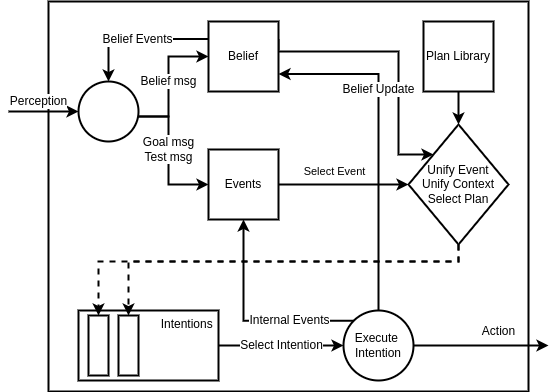
\includegraphics[width=0.70\linewidth]{ch_agere/asc2arch.drawio.png}
  \caption{ASC2's functional architecture}
  \label{fig:asc2func}
\end{figure}


Taking the example script in Listing~\ref{lst:domestic_robot}, Suppose the agent receives and event in the form of: 
\begin{minted}[fontsize=\small]{prolog}
!go_order(french,meal(veg,meat,white))
\end{minted}
\noindent For this event, plan P1 is relevant with unifier:
\begin{minted}[fontsize=\small]{prolog}
{Loc/french, Meal/meal(veg,meat,white)}
\end{minted}
Then applying this unifier to the context condition of that plan will result in the expression:
\begin{minted}[fontsize=\small]{prolog}
restaurant(french) & not at(french)
\end{minted}
Which indeed is a logical consequence of the agents beliefs, meaning this plan is applicable with the same unifier as before (i.e., the query does not add any new substitutions). Then, by applying this substitution to the plan itself will result in:
\begin{minted}[fontsize=\small]{prolog}
+!go_order(french,meal(veg,meat,white)) :
    restaurant(french) & not at(french) =>
    #move_to(french);
    !order(meal(veg,meat,white)).
\end{minted}

The steps in the body of the instantiated plan become an intended means for the agent to execute. The first step \asc{#move_to(french)} is simply a function call. In ASC2, this could be any callable entity on the JVM's execution classpath. In this example we are assuming that this call somehow relocates agent to the location specified as the parameter. The second step is \asc{!order(meal(veg,meat,white))} which is a sub-goal. In functional terms a sub-goal is processed by the agent as an internal event that will follow the same plan selection process.

This process is better described in ASC2 as a reasoning flow instead of a reasoning cycle. This is because unlike what is typically the case in BDI frameworks, ASC2 does not implement an explicit synchronous reasoning cycle. As a result the two selection functions $S_E$ and $S_I$ are asynchronous: when an event arrives, it will be processed in an asynchronous manner given there are free resources available to the agent. Or, when a new intent is created, it will be executed asynchronously given there are free resources available. In effect, the sets $E$ and $I$ are priority queues and $S_E$ and $S_I$ are sorting functions that define the priority of the entities in these queues. The default implementation for both is a simple first-in-first-out (FIFO) algorithm. A new event or an intention will be selected by their respective selection function when processing resources, namely threads from a thread pool become available.



% As this work focuses on the goal refinement, the following formal definitions namely plans, relevant plans, and applicable plans are reiterated from \cite{RaoAS1996}. 





% \Gio{[here we should write a bit about variables, constants, unification and unifiers.]}
% \Mos{Giovanni can write this}


%\noindent For the given definitions, only relevant plans may be applicable. 

% \paragraph{Domestic Robot Agent}
% To demonstrate the full functional plan instantiation process of our agent, imagine a domestic robot that upon request can go to a restaurant and order a three course meal. The script for such agent is presented in Listing \ref{lst:domestic_robot_1}. 
% %\footnote{In the excerpts we modified slightly the AgentSpeak(L) syntax, replacing ``\texttt{<-}'' with ``\texttt{=>}'', to further distinguish the reactive, forward nature of these rules w.r.t. the backward chaining derivation of Prolog rules ``\texttt{:-}''.} 
% The agent has two plans for going to a restaurant and ordering a meal, the first plan (P1) is \textit{applicable} if the agent is not at a restaurant at the moment, which means a step of moving (\asc{#move_to} primitive action) is needed prior to ordering the meal, the second plan (P2) is applicable if the agent is already at the restaurant which means the agent will just adopt the goal of ordering the meal. There is also one plan for ordering the meal (P3) which is applicable if the agent has the belief that the meal it wants to order exists.

% \begin{listing}[t]
% \centering
% \begin{minted}[fontsize=\small]{prolog}
% % initial beliefs
% main(fish). main(meat). soup(veg). soup(fish).
% wine(white). wine(red).
% restaurant(french). restaurant(italian).
% at(home).
% % inferential rules
% meal(S,M,W) :- soup(S), main(M), wine(W).

% % plans
% % P1
% +!go_order(Loc,Meal) :
%         restaurant(Loc) && not at(Loc) =>
%         #move_to(Loc);
%         !order(Meal).
% % P2
% +!go_order(Loc,Meal) :
%         restaurant(Loc) && at(Loc) => 
%         !order(Meal). 
% % P3
% +!order(meal(S,M,W)) : 
%         meal(S,M,W) => 
%         #ask_waiter(meal(S,M,W)).
% \end{minted}
%     \caption{Domestic robot agent's script}
%     \label{lst:domestic_robot_1}
% \end{listing}%
% \noindent Suppose the agent receives and event in the form of: 
% \begin{minted}[fontsize=\small]{prolog}
% !go_order(french,meal(veg,meat,white))
% \end{minted}
% It will put it in the event queue, assuming this is the only event the agent selects it for processing. For this event, both plans (P1) and (P2) are relevant with unifier $\sigma$:
% \begin{minted}[fontsize=\small]{prolog}
% {Loc/french, Meal/meal(veg,meat,white)}
% \end{minted}
% Assuming that the belief base of the agent contains the beliefs \asc{restaurant(french)} (meaning that there exists a French restaurant) and \asc{at(home)} (meaning that the agent is at home), then only the first plan will be an applicable plan for this event, and the applicable unifier will be the same as the relevant unifier. This entails that only plan (P1) will be instantiated as: 
% \begin{minted}[fontsize=\small]{prolog}
% +!go_order(french,meal(veg,meat,white)) :
%     restaurant(french) & not at(french) =>
%     #move_to(french);
%     !order(meal(veg,meat,white)).
% \end{minted}

% As a next step, this instantiation becomes an intention of the agent, and assuming it is the only intention, the agent selects it for execution, the first step \asc{#move_to(french)} is simply a function call. In ASC2, this call could be any callable entity on the JVM's execution classpath. In this example we are assuming that this call somehow relocates agent to the location specified as the parameter. The second step is \asc{!order(meal(veg,meat,white))} which is a sub-goal. In functional terms a sub-goal is processed by the agent as an internal event that will have the same plan and intention selection process.


% Note that in case the agent at any step had more than one event to select from, more than one plan or applicable unifier, or more than one intention, then the selection function would have been called to select one of the options.


\subsubsection{ASC2 Structural Architecture}
The structural architecture of ASC2 agents is based on the Actor model. Each agent consists of multiple actors with different roles: (\romannumeral 1) an \textbf{Interface} actor, (\romannumeral 2) a \textbf{Belief Base} actor, (\romannumeral 3), an \textbf{Intention} \textbf{Pool} actor and (\romannumeral 4) $N \ge 1$ \textbf{Intention} actors. Each agent has also non-actor components: (1) a plan library, and (2) one or more belief bases. An overview of this architecture is presented in Figure~\ref{fig:asc2arch}.
%\begin{itemize}
%    \item An Interface actor
%    \item A Belief Base actor
%    \item An Intention pool actor
%    \item $N \ge 1$ Intention actors
%\end{itemize}

The plan library of the agent consists of a set of plan rule objects in the form \verb+{e,c,h}+, where \verb+e+ is an object that can be matched and unified with event messages to determine if a plan rule is relevant for that event, \verb+c+ is an expression object that can be sent to the Belief Base actor to determine if the plan is applicable and \verb+h+ is a function representing the body of the plan.

The belief base(s) of the agent can be in practice any type of storage technology. To interface an arbitrary belief base into the agent architecture a translation function needs to be implemented for mapping the query messages into the queries of that belief base and vice versa, translating the responses into result messages.\footnote{For the benchmarks presented in this work we used a lightweight open-source Prolog reasoning engine implemented in Scala called \textit{Styla}, available at \url{https://github.com/fedesilva/styla}. %, % \cite{Styla}
The library was minimally modified and is available at \url{https://github.com/mostafamohajeri/styla}.}

\begin{figure}[t!]
  \centering
  \includegraphics[width=0.70\linewidth]{ch_agere/arch3.png}
  \caption{ASC2's structural architecture}
  \label{fig:asc2arch}
\end{figure}

\subsubsection{Interface Actor}
The Interface actor acts as the main entity of the agent. It initializes the Belief Base and Intention Pool actors and then sends the initial beliefs and inferential rules to Belief Base actor as \textit{assert} messages and initial goals to Intention pool actor as \textit{achieve} messages. This actor is the only component of the agent that is accessible from the environment and the other agents: all incoming messages and events must go though this actor and any message sent from this agent will indicate the Interface actor as the sender of message. When the Interface actor receives a new message $m$, based on the type of the message it will either process it itself if $m$ is a control messages, (e.g, \textit{halt}), forward it to Belief Base actor if $m$ is an assert message (e.g, \textit{perception}) or forward it to Intention Pool actor if $m$ is an achieve message (e.g, \textit{request}).



\subsubsection{Belief Base Actor}
The Belief Base actor maintains the connection between other components of the agent and any data storage/reasoning engine that is used as the belief base. This actor accepts query messages (\textit{retract}, 
\textit{assert} and \textit{unify}) and responds with result of the query. The technology of the data storage(s) is abstracted behind this actor and it can be changed by the programmer without affecting the rest of the framework. The specific implementation of the belief base is injected to the agent initialization time. % Note that also inferential rules can be seen as \textit{integrity constraints} that the belief base is required to enforce. 
Apart from processing queries, the Belief Base actor also feeds back \textit{belief-update} events to the Interface actor. The semantics of when these events should be created are externalized to the core of architecture and can be programmable by the designer. This is the inversion of control as the belief base can control other components by sending messages to them.

\subsubsection{Intention Pool actor}
The Intention Pool actor receives events from the Interface actor and processes them. To process a received event \verb+v+, the set of relevant plan rules \verb+{e,c,h}+ are selected from the plan library by matching and unifying \verb+v+ against \verb+e+. Then these relevant plans are fetched from the plan library and sent to an idle Intention actor. The Intention pool actor can spawn $N$ Intention actors, where the configurable number $N$ dictates the number of concurrent intentions each agent can have at each instant. This actor uses a prioritized mailbox that sorts the messages based on the externalized programmable priority function $S_E$ and a new event is processed only if there are idle Intention actors to forward it to. This mechanism makes sure that as long as there are no resources available, new events stay in the mailbox to be re-prioritized by $S_E$ and when an idle Intention actor becomes available the event with the highest priority is processed \footnote{In the current implementation, the Intention pool actor exploits the \textit{Router} feature of Akka.}. % is used to implement the Intention pool actor.

\subsubsection{Intention Actor}
An Intention actor is a reusable unit of execution for the agent. It receives an event \verb+v+ alongside a set of plan rule objects \verb+{e,c,h}+ from the Intention Pool actor for execution. The execution consists of three phases: (\romannumeral 1) the applicability of each plan rule is checked by sending a query message containing \verb+c+ to the Belief Base actor; (\romannumeral 2) from the set of applicable plans, one is selected by the externalized programmable function $S_P$ for execution; (\romannumeral 3) the function  \verb+h+ of the selected plan is executed by the Intention actor. After the execution of \verb+v+ is completed either by success or failure status, a message is sent to the actor which originally requested \verb+v+ containing the completion status and also a message is sent to Intention Pool actor signaling that this actor is now idle.


\subsection{Translation Method}
The translation method is designed to compile the models specified with the ASC2 DSL described in \ref{section_dsl} into agents with the architecture described in \ref{section_arch}. 

For each entity of the DSL, a mapping is defined to generate the code in the executable underlying language that can instantiate the objects with the desired semantics at run-time. The translated entities are then fitted in the abstract architecture to form an executable agent program.

\subsubsection{Terms and Expressions}
The ASC2 DSL uses Prolog-style terms and expressions. In the translation of an script written in the DSL, each term and expression (including inferential rules) maps to a \verb+Term+ or \verb+Expression+ object which encapsulates the parsed data (potentially containing nested \verb+Term+s and \verb+Expression+s).

Any expression in ASC2 can be translated and analysed in two ways: (1) external to the script by querying the belief base, and, (2) locally as part of the low-level code. The first approach makes use of any data-storage engine utilized by the belief base. This process is by default present in checking the context conditions of plans, but can also be used at any point in the agent's script; in our example the expression:
\begin{minted}[fontsize=\small]{prolog}
restaurant(Loc) && not at(Loc)
\end{minted}

\noindent can both be checked against the belief base to check if it can be proven, also a substitution for the variable \asc{Loc} will be returned ---that is if the belief base uses a prolog-like reasoning engine. In any case, this type of expression utilizes the full capacity of the belief base which can also be less efficient. The translated Scala version of this expression is illustrated in following, note that this is simply an object instantiation that can be analysed by the belief base's reasoning engine:
\begin{minted}[fontsize=\small]{java}
StructTerm(",",
    Seq(StructTerm("restaurant",
            Seq(vars("Loc"))),
        StructTerm("not",
            Seq(StructTerm("at",Seq(vars("Loc")))))))
\end{minted}

The second type are expressions that can be calculated locally, and for example are used in control flow structures \asc{if/else} or variable assignments. As an example, if in the context of execution of a plan we have a variable \asc{Loc} that is grounded by the string value \asc{"french"}, the statement:
\begin{minted}[fontsize=\small]{prolog}
Loc + "_restaurant" == "french_restaurant"
\end{minted}
\noindent can be calculated locally to boolean value \asc{true} ---e.g., in a variable assignment statement--- without the need to query the belief base. Intuitively this second approach does not utilize the capabilities of the belief base but the local nature of its translation ---it is calculated locally by the underlying language--- can be very efficient. The translated Scala version of the second expression is, not that unlike before this is already an expression that can be calculated by JVM without the need for any extra reasoning\footnote{Alongside some implicit type conversions}:
\begin{minted}[fontsize=\small]{java}
(vars("Loc") + StringTerm("_restaurant"))  ==
    StringTerm("french_restaurant"))
\end{minted}


\paragraph{Access to the Lower-Level Language} As consequence of an approach based on compilation, the DSL provides direct access to any object or function available in the agent's name space ---in the Scala implementation, any object or function which is accessible via the Java class path. These lower-level access statements, indicated by the token \verb+#+, are translated literally to the same statement in the underlying language. This capability provides fast and seamless reuse of libraries already established for the underlying language. Let us take the previous example, but this time also use a few of JVM's basic library methods, namely \asc{String.join} and \asc{String.toUpperCase}:
\begin{minted}[fontsize=\small]{prolog}
#String.join("_", Loc, "restaurant").toUpperCase == "FRENCH_RESTAURANT"
\end{minted}
\noindent which translates to the valid Scala statement:
\begin{minted}[fontsize=\small]{java}
String.join(StringTerm("_"),
            vars("Loc"),
            StringTerm("restaurant"))
                .toUpperCase == 
                    StringTerm("FRENCH_RESTAURANT"))
\end{minted}
 %alongside implicit and explicit type conversions,

\subsubsection{Initial Beliefs/Goals and Inferential Rules}
At syntactic level, initial beliefs and inferential rules are logic-style expressions, and as such they translate to an \asc{Expression} object counterpart. Initial goals are a combination of a prefix (\asc{!}, designating the adoption of a new goal)
and a term and they translate to a \asc{Goal} object encapsulating the prefix and a \asc{Term} object. At initialization time, the initial beliefs are sent to the Belief Base actor to be asserted and initial goals are adopted sequentially in a synchronous manner, i.e., there is no concurrency.

\subsubsection{Plan Rules}
A plan rule $<e,c,h>$, should be translated into the object \asc{{e,c,h}} which will be part of the plan library. The triggering event of the plan rule $e$ consists of a trigger (one of \asc{+!,-!,+?,+,-}) and a term $t$. The triggers convey the relevance of the plan to different event types while $t$ can be seen as the payload of that event; \verb#+!# relates to adoption of a new goal, \verb#-!# relates to failure of a goal, \verb#+?# relates to test goals, \verb#+# and \verb#-# respectively relate to assertion and retraction of a belief. The triggering event $e$ then translates to an \asc{Event} object which encapsulates the trigger and the translated \asc{Term} object of $t$. The context condition $c$ is an expression and translates to an \asc{Expression} object which can be sent to the Belief Base actor in a synchronous manner, and the response to that message determines if the plan is applicable in the current context and also returns the substitution for the variable (if any). The plan body $h$ of a plan rule consist of zero or more steps. %and each step can be one of the plan step types. 
%The plan body 
It is translated into a function \verb+h+, which contains the steps of $h$ as imperative lines of code implemented in it. Each type of step is translated differently as is described below.



\paragraph{Primitive Actions}
A primitive action of the form \asc{#h(...)} is in practice a lower-level function call in the underlying language and it %for an agent 
is translated into a call to a function \asc{h(...)} with its respective parameters. In the case of Java/Scala, this can be any callable entity on JVM's \textit{classpath}. Take for example Scala's \asc{println} method, to call this method as a primitive action a simple \asc{#println("hello")} can be a statement used in ASC2, and a translation of this call will be:
\begin{minted}[fontsize=\small]{java}
primitive_handler.execute(() => println(StringTerm("hello")))
\end{minted}
\noindent Note that in this translation the object \asc{primitive_handler} is a dependency of the agent that in its default implementation simply calls the function passed to it, but, can be potentially customized and injected to the agent for more flexible control on what and how the functions are being called.

However, often the designer will need to define new domain specific methods to call from the agent's script as primitive actions, and these methods need access to the execution context of the agent itself. In every block of code in the translated code, there is an implicit value \footnote{This specifically refers to Scala's implicit values, these values do not need to be passed explicitly in a function call, instead if the corresponding method has declared them as an implicit parameter in its signature, Scala will automatically look for them and pass them along as a parameter.} called \asc{executionContext} that contains the information about the agent and its execution context. This object contains information varying from simple attributes e.g., agent's name and type, to more technical information e.g., the current thread the function was called in, to even higher level information e.g., the intention or goal that was the source of the call or even on which agent's request this goal was adopted. To access this object from the context of a primitive action, the designer merely needs to declare it as an implicit parameter for the corresponding method. Take for example a simple primitive action that prints the agent's name and can be called from the script as \asc{#print_name}, the implementation for this function will be:
\begin{minted}[fontsize=\small]{java}
def print_name()(implicit executionContext: ExecutionContext) =
    println(executionContext.name)
\end{minted}

One of the most important advantage about how ASC2 handles primitive actions is that they do not need to be implemented in any specific class nor do they need to be passed to the agents at initialization time. This makes the development of agents and MAS much more scalable as primitive actions in a domain and the agent's scripts are completely isolated: the \asc{#print_me} action can be built, packaged as a JVM artifact and placed in an artifact repository, then, it can simply be utilized by other designers by importing that artifact in a project\footnote{The more detailed exploration of development ecosystem in ASC2 is illustrated in Chapter~\ref{ch:emas}}.

% Like other low-level access statements these can be any function available on the name space of the agent's object. 
% A step that is indicated by the parser as a primitive action, is translated into a function call 

\paragraph{Variables and Assignment Statements}
Variable assignment statements in form of \verb+V = exp+ are used to (re-)assign the result value of an expression \verb+exp+ to a variable \verb+V+. ASC2 uses an internal map-like approach to store variables that also manages variable scopes, meaning that each code block (e.g, plan body, condition block) holds a map of all variables declared in that scope which also inherits the variables in its parent scope. Every read/write to a variable \asc{V} then becomes a read/write operation to a member of the variable's map with the key \asc{"V"}. A variable assignment is translated to an (overwriting) append operation for the variable's map by using the $V$ as the key and \verb+exp+ as the value. As an example the statement \asc{V = V + 1} is translated to:

\begin{minted}[fontsize=\small]{java}
vars += ("V" ->  (vars("V") + IntTerm(1)))
\end{minted}
\paragraph{Belief Updates}
Belief update steps are composed of a prefix \verb|+,-| and a term $t$. The prefixes respectively mean assertion and retraction. As the belief base of the agent is abstracted by the Belief Base actor, a belief update step is a blocking message to the Belief Base actor about assertion or retraction of the \verb+Term+ object of $t$. At a practical level, after translation belief-updates are technically low-level calls to a specific function, take for example the statement \asc{+at(home)}, when translated becomes:
\begin{minted}[fontsize=\small]{java}
belief_handler.execute(
    Belief.ASSERT,
    StructTerm("at",Seq(AtomTerm("home"))))
\end{minted}
In this code the object \asc{belief_handler}  is a dependency of the agent that in its default implementation performs the aforementioned messaging with the Belief Base actor, but, can be potentially customized and injected into the agent for more flexible control on how belief updates are handled. Furthermore, ASC2 agents also react to belief-update triggers that may happen by assertion or retraction of a belief, however that process is completely controlled by the Belief Base actor that in its default implementation when a belief is asserted or retracted sends event messages to the Interface actor; this process can be customized by the designer\footnote{At this point it may seem this much flexibility is not a requirement for a BDI framework. Evidently, most BDI frameworks are designed with the assumption of using a prolog-like backward-chaining query-response belief base. However, there are many interesting experiments that can be performed if that was not a limitation, an example illustrated in Chapter~\ref{ch:norm} where the belief base of the agents is replaced with a forward chaining norm reasoner that is continuously producing normative events for the agent.}.

\paragraph{Sub-Goal Adoption}
Task decomposition is crucial component of BDI-like agents and in essence is the ability to adopt sub-goals depending on the context of a plan. At the syntactic level, a (sub-)goal adoption is a prefix (e.g, \verb+!,?+) plus a term $t$. The prefixes respectively mean achievement and test goals. In the translation method a sub-goal adoption step is translated as two phases, (\romannumeral 1) a plan selection by using $S_P$ is done to select and fetch a plan rule object \verb+{e,c,h}+ from the plan library, (\romannumeral 2) the function \verb+h(...)+ is called with any parameters that $t$ may have as the arguments of \verb+h+.

\paragraph{Control Flow Structures}
The compilation method of ASC2 supports a  straightforward mapping of simple control flow structures such as loops and conditionals to their executable counterparts. The translation of these control structures to the underlying language is performed one-to-one; for example an \verb+if/else+ in the DSL is simply translated to an \verb+if/else+ in the underlying language.

\subsection{Tools for Execution}
The architecture of ASC2 agents is based on actors and for their execution these actors require an \textit{actor system} that \textit{spawn} and \textit{start} them. The implementation of ASC2 is written in Scala and is based on the Akka framework. In addition to a compiler\footnote{Source code: 
\url{https://github.com/mostafamohajeri/scriptcc-translator}.}, it includes a minimal infrastructure that is able to spawn and start the compiled agents% \cite{CCTranslator}
\footnote{Source code: \url{https://github.com/mostafamohajeri/agentscript}.
%of the execution framework can be found in \cite{AgentScript}
}.

\paragraph{Communication Interface}
All the external communications of the agent are transmitted through one (or more) \textit{transportation layer}. This layer needs to be specified to enable communication between agents. The framework remains agnostic with respect the transportation layer as long as there is an interface to convert messages from and to ASC2's message protocol. The default transportation layer makes use of Akka's typed messages. However, this layer is one of the dependencies that is injected into the agents at initialization time. This allows the designer to implement this layer with any technology (e.g., REST API, gRPC, Message Queues) and inject it into agents to allow them to communicate with other agents (and other entities) using that technology without the need to modify the framework or even the script of the agents.

The communications interface of the agents is based on speech act preformatives. On a practical level, they are implemented with actions like \mintinline{text}{#achieve} which relays an achievement goal event, \mintinline{text}{#tell} and \mintinline{text}{#untell} which relay belief-update events, and \mintinline{text}{#ask}/\mintinline{text}{#respond} which can be used between agents as synchronous communication with test goal events.


\section{Performance Analysis}
\label{sec_bench}

The following section proposes quantitative comparisons between the ASC2 framework and three other frameworks: Jason (\verb+v2.5+), ASTRA (\verb+v1.0.0+) and Sarl (\verb+v0.11.0+). Jason \cite{Bordini2005} was chosen because, like ASC2, it uses a language based on AgentSpeak(L), is implemented in Java and as reported by \cite{Cardoso2013} potentially outperforms other BDI frameworks. ASTRA and Sarl are both also implemented in Java, but, more importantly, like ASC2, rely on a compilation approach. %which makes them a good candidate for comparison.

Performance comparison is effectuated by means of two fairly standard benchmarks (token ring, chameneos redux), close to what has been presented in \cite{Cardoso2013}. The main difference w.r.t. \cite{Cardoso2013} is the metrics, as we separate the interpretation/setup time from the execution time, to present better insights on how these frameworks operate. %while in \cite{Cardoso2013} they are considered together. 
An additional benchmark (service point) was also performed to assess the ability of the frameworks to allow concurrent decomposition of tasks inside the agents. The benchmarks were performed on a {Debian GNU/Linux 10} machine with an 8 core {Intel(R) Xeon(R) CPU E5-1620 v4 @ 3.50GHz} CPU and {64GB} of RAM using Java version {11} with {GraalVM 20} JRE.  Each benchmark was performed $10$ times and the JVM was stopped between each run to avoid the impact of one experiment on the next. %The results are further discussed in section \ref{sec:discussion}.

In the first two benchmark scenarios, three metrics are recorded: (1) total interpretation/setup time, including agent creation time, (2) internal execution time measured from the instant that the first agent starts until the completion of the test, and (3) CPU core load. Execution and data gathering is controlled by a Python script that runs the benchmarks in the desired dimensions and records the metrics\footnote{Source code: \url{https://github.com/uva-cci/aop-benchmarks-agere2020}.}. %(4) total memory usage and the result of each metric is presented for each framework.
%In each benchmark two variations of ASC2 are tested, a \textit{script} and a \textit{compiled} version. In the script version the program starts with the scripts written in the DSL and the whole parsing and run-time compilation is also taken as part of setup time. In the compiled version the program is already parsed and built with a build tool. Sarl and ASTRA provide build tools to export executable applications, and also in their case we used an already built program to benchmark the execution.

\subsection{Token Ring}
The token ring benchmark is a simple program targeting multiple aspects of parallel frameworks: handling different number of agents, message passing and level of concurrency each agent can achieve. The testing scenario consists of $W$ worker agents, $T$ tokens are distributed among the workers, and each token has to be passed $N$ times in a ring. When all $T$ tokens have been passed $N$ times, the program ends. To run this benchmark a program should:
\begin{itemize}
    \item create $W$ number of workers;
    \item each worker should be connected to its neighbor forming a complete ring;
    \item initially each token $1\leq i \leq T$  is assigned to a worker $1\leq j \leq W$ with the equation $j = i * (W/T)$
    \item each worker sends the token to its neighbor
\end{itemize}
The program finishes when all $T$ tokens have been passed $N$ times.

The experiment was performed by varying $W$, $T$ and $N$ independently within the values $\{4,16,256,1k,4k\}$, resulting in $125$ different configurations for each framework. We also put a $1$ minute limit for each execution and anything beyond that is considered a \textit{timeout}. 

\subsubsection{Implementation Notes} In all implementations a \textit{broker} agent is present that starts the benchmark by distributing the tokens and gathers the completed tokens to stop the execution. There is a difference in the Sarl implementation. As Sarl does not provide a central agent resolver to address agents by name, an extra step is implemented in the broker to iterate over all worker agents and link them together in a ring.

\subsubsection{Results} 
A summary of the results for this benchmark is presented in Figures \ref{fig:token1} and \ref{fig:token2}. In Figure \ref{fig:token1}, the number of agents $W$ is the variable while $N$ and $T$ are kept constant with two settings $(N=256,T=256)$ and $(N=4k,T=4k)$. Only Jason and ASC2 were able to execute $(N=4k,T=4k)$. Sarl was able to only execute the benchmark up to $W=256$ agents and timed out with a warning\footnote{Potentially dangerous stack overflow in \texttt{java.util.concurrent.locks} \texttt{.ReentrantReadWriteLock}. We suspect this occurs because at the start all workers need to send a message to the broker to get their neighbors and the broker can not handle this amount ($\ge1024$) of concurrent messages.}. ASTRA seemed stable enough to finish the $(N=4k,T=4k)$ test but not within $1$ minute. ASTRA executes very poorly for $(N=256,T=256)$ test, especially with lower number of worker agents, plausibly because with less worker agents each agent has more concurrent threads of work to execute. ASC2 and Jason both perform almost without much effect w.r.t. number of agents, suggesting that both frameworks can handle concurrency inside agents to a good extent, although in all cases Jason performs marginally better.

In Figure \ref{fig:token2} another view on the results is presented. This time the variable is the number of tokens $T$, whereas $W,N$ are kept constant in two settings:  $(W=256,N=256)$ and $(W=4k,N=4k)$. Like in the previous results Sarl could only finish the $(W=256,N=256)$ test. ASTRA was able to execute the $(W=4k,N=4k)$ test but only up to $T=1k$ and timed out after that. In the $(W=256,N=256)$ Jason and ASC2 performed much better and scaled almost linearly with the number of tokens which shows that both frameworks can handle the increased concurrency and the higher number of messages to be passed in an efficient manner. On the other hand Sarl and ASTRA performed poorly under the increasing amount of tokens. In the $(W=4k,N=4k)$ test Jason performs marginally better than ASC2.

\paragraph{CPU Load} Figure \ref{fig:cpu_load_token1} and Figure \ref{fig:cpu_load_token2} present the average core load during the token ring test respectively in the $W,T=256$ and $N=4096$ and in the $W,T,N=4k$ settings. % for each framework is presented and in Figure \ref{fig:cpu_load_token2} the average core load for the  setting is shown. % As it can be seen 
In the lower settings (Figure \ref{fig:cpu_load_token1}) Jason and ASTRA have much less CPU demand than ASC2 and Sarl. On the other hand, in the higher setting (Figure \ref{fig:cpu_load_token2}) the CPU load between Jason and ASC2 is closer (respectively $85.7\%$ and $88.6\%$, vs $57.7\%$ and $77.7\%$ in the lower setting). %with ASC2 averaging at $88.6\%$ and Jason at $85.7\%$ while they respectively averaged at $77.7\%$ and $57.7\%$ in the lower setting. 
This can be an indication that ASC2 has a higher footprint on the CPU load, especially for initialization time. 

To understand how much each framework can distribute the load between CPU cores we have to look at the standard deviation of CPU load data. A higher deviation % from average 
indicates that the framework is not balancing the load between cores. ASTRA shows to have very poor load balancing with the deviation almost as high as the average which can mean that some of the cores are not even used in execution. Sarl has a high balancing of cores even in lower setting. In the higher settings both Jason and ASC2 seem to distribute the load between CPU cores sufficiently.

\paragraph{Initialization Time}
To assess the initialization time, total execution time is subtracted by the internal execution time in the lowest setting with $N=4k$ and $T=4k$ and the results are presented for an increasing number of agents in Figure \ref{fig:init1}. ASTRA proves to have the fastest initialization, at least up to $4k$ agents, followed by Jason and closely by ASC2. Sarl seems to have the slowest initialization time and scales very badly with the number of agents. 

\begin{figure}[tb!]
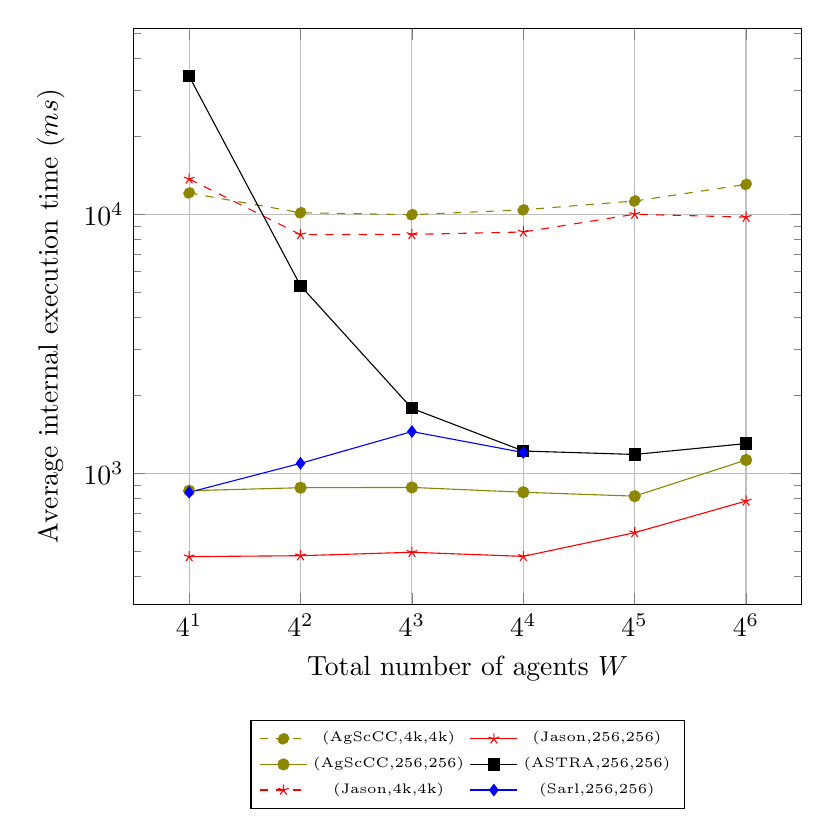
\begin{tikzpicture}
\begin{axis} [
scale only axis,
    width=0.70\textwidth,
    grid=major,
    transpose legend,
		legend columns=3,
		legend style={at={(0.5,-0.2)},anchor=north,font=\tiny},
    xmode=log,
    log basis x={4},
    ymode=log,
    log basis y={10},
    xlabel={Total number of agents $W$},
    ylabel={Average internal execution time ($ms$)},
    % cycle list name=
]
\addplot[mark=*,olive,dashed,error bars/.cd,y dir=both,y explicit
    ]
    coordinates {
(4 , 12064.0) %+- (654.172080657002 , 654.172080657002)
(16 , 10118.9) %+- (350.159471606232 , 350.159471606232)
(64 , 9943.9) %+- (233.08341377665155 , 233.08341377665155)
(256 , 10383.7) %+- (395.6162703091638 , 395.6162703091638)
(1024 , 11228.4) %+- (284.6249774313171 , 284.6249774313171)
(4096 , 13013.5) %+- (1324.0409736862375 , 1324.0409736862375)
    };
    \addlegendentry{(AgScCC,4k,4k)}
    
    \addplot[mark=*,olive,error bars/.cd,y dir=both,y explicit
    ]
    coordinates {
(4 , 857.1) %+- (98.22134866378761 , 98.22134866378761)
(16 , 880.3) %+- (70.18396461364155 , 70.18396461364155)
(64 , 882.6) %+- (119.83340287434235 , 119.83340287434235)
(256 , 845.5) %+- (105.0124331263261 , 105.0124331263261)
(1024 , 816.8) %+- (42.871383877308595 , 42.871383877308595)
(4096 , 1126.1) %+- (124.52170716608231 , 124.52170716608231)
    };
    \addlegendentry{(AgScCC,256,256)}
    
 
    \addplot[mark=star,red,dashed,error bars/.cd,y dir=both,y explicit
    ]
    coordinates {
   (4 , 13658.3) %+- (252.6855973559061 , 252.6855973559061)
(16 , 8329.5) %+- (164.36291146930523 , 164.36291146930523)
(64 , 8345.8) %+- (150.9273555942284 , 150.9273555942284)
(256 , 8527.7) %+- (150.2908661377811 , 150.2908661377811)
(1024 , 9984.2) %+- (209.81356803918408 , 209.81356803918408)
(4096 , 9729.8) %+- (1202.9822028678224 , 1202.9822028678224)
    };
    \addlegendentry{(Jason,4k,4k)}
    \addplot[mark=star,red,error bars/.cd,y dir=both,y explicit
    ]
    coordinates {
(4 , 477.4) %+- (13.133502536981096 , 13.133502536981096)
(16 , 481.3) %+- (14.14252845537569 , 14.14252845537569)
(64 , 496.3) %+- (22.90584593019384 , 22.90584593019384)
(256 , 478.5) %+- (23.665492928640965 , 23.665492928640965)
(1024 , 590.6) %+- (28.47298914956263 , 28.47298914956263)
(4096 , 782.5) %+- (30.938110263341336 , 30.938110263341336)
};
    \addlegendentry{(Jason,256,256)}
        \addplot[mark=square*,black,error bars/.cd,y dir=both,y explicit
    ]
    coordinates {
(4 , 34001.7) %+- (771.5794839159475 , 771.5794839159475)
(16 , 5293.5) %+- (330.20540745286274 , 330.20540745286274)
(64 , 1780.7) %+- (23.002656851377456 , 23.002656851377456)
(256 , 1219.4) %+- (27.597101297056543 , 27.597101297056543)
(1024 , 1182.8) %+- (18.972494710911253 , 18.972494710911253)
(4096 , 1302.7) %+- (29.95570804445197 , 29.95570804445197)

        };
    \addlegendentry{(ASTRA,256,256)}
    
       
    \addplot[mark=diamond*,blue,error bars/.cd,y dir=both,y explicit
    ]
    coordinates {
    (4 , 845.2222222222222) %+- (154.7447719454342 , 154.7447719454342)
    (16 , 1093.111111111111) %+- (619.9662177176359 , 619.9662177176359)
    (64 , 1449.5) %+- (790.6629075233853 , 790.6629075233853)
    (256 , 1203.2) %+- (1067.3895258995192 , 1067.3895258995192)
    };
    \addlegendentry{(Sarl,256,256)}
    

\end{axis}
\end{tikzpicture}
\caption{Token ring results for each (framework, $T, N$)}
\label{fig:token1}
\end{figure}%
\begin{figure}[tb!]
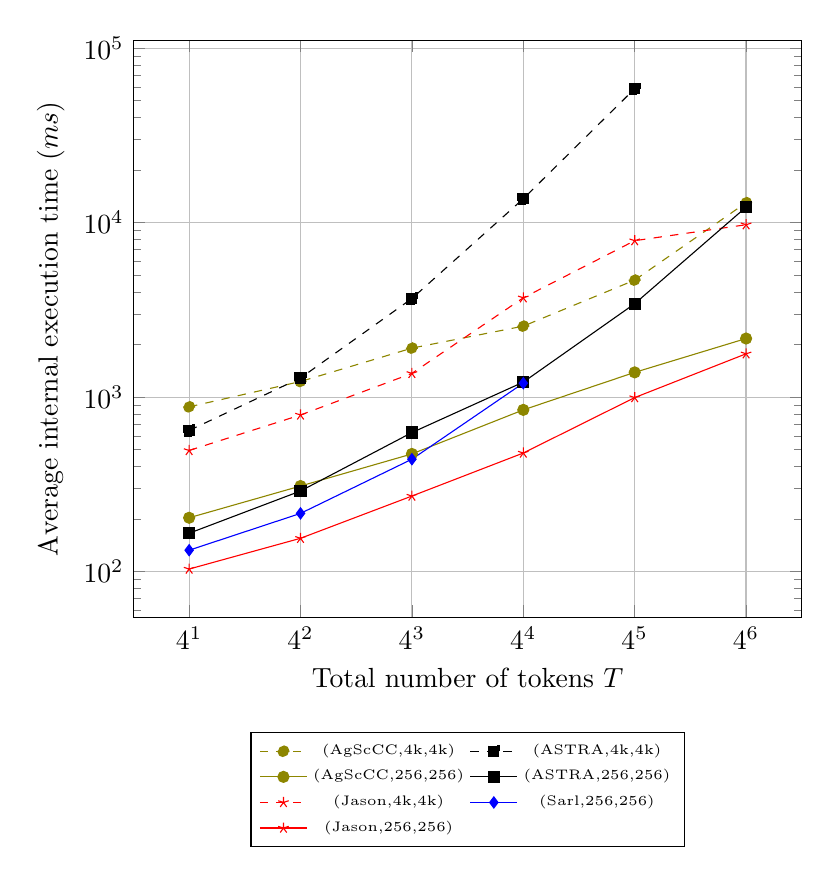
\begin{tikzpicture}
\begin{axis} [
scale only axis,
    width=0.7\textwidth,
    grid=major,
    transpose legend,
		legend columns=4,
		legend style={at={(0.5,-0.2)},anchor=north,font=\tiny},
    xmode=log,
    log basis x={4},
    ymode=log,
    log basis y={10},
    xlabel={Total number of tokens $T$},
    ylabel={Average internal execution time ($ms$)},
    cycle list name=black white
]

\addplot[mark=*,olive,dashed
    ]
    coordinates {
    (4 , 879.8)
(16 , 1229.2)
(64 , 1909.6)
(256 , 2552.4)
(1024 , 4684.5)
(4096 , 13013.5)
    };
    \addlegendentry{(AgScCC,4k,4k)}
    
    \addplot[mark=*,olive
    ]
    coordinates {
    (4 , 203.6)
    (16 , 309.5)
    (64 , 472.7)
    (256 , 845.5)
    (1024 , 1386.8)
    (4096 , 2167.5)
    };
    \addlegendentry{(AgScCC,256,256)}
    \addplot[mark=star,red,dashed
    ]
    coordinates {
    (4 , 494.8)
(16 , 790.4)
(64 , 1368.1)
(256 , 3710.7)
(1024 , 7884.8)
(4096 , 9729.8)
    };
    \addlegendentry{(Jason,4k,4k)}
    \addplot[mark=star,red
    ]
    coordinates {
    (4 , 103.5)
(16 , 155.3)
(64 , 271.2)
(256 , 478.5)
(1024 , 994.2)
(4096 , 1772.2)
};
    \addlegendentry{(Jason,256,256)}
    
    \addplot[mark=square*,black,dashed
    ]
    coordinates {
    (4 , 644.4)
(16 , 1287.1)
(64 , 3674.8)
(256 , 13711.6)
(1024 , 58593.0)
        };
    \addlegendentry{(ASTRA,4k,4k)}
    
        \addplot[mark=square*,black
    ]
    coordinates {
    (4 , 166.0)
(16 , 289.8)
(64 , 626.6)
(256 , 1219.4)
(1024 , 3432.0)
(4096 , 12273.7)
        };
    \addlegendentry{(ASTRA,256,256)}
    
       
    \addplot[mark=diamond*,blue
    ]
    coordinates {
    (4 , 132.7)
    (16 , 215.7)
    (64 , 440.9)
    (256 , 1203.2)
    };
    \addlegendentry{(Sarl,256,256)}

\end{axis}
\end{tikzpicture}
\caption{Token ring results for each (framework,$W,N$)}

\label{fig:token2}
\end{figure}


\begin{figure}
    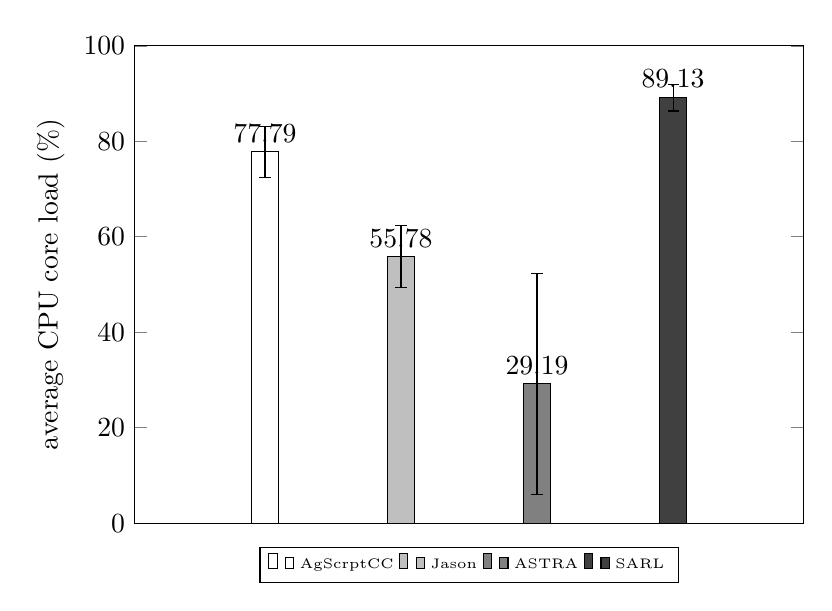
\begin{tikzpicture}
\begin{axis}[
    scale only axis,
    height=0.5\textwidth,
    width=0.7\textwidth,
    ybar,
    enlarge x limits=0.15,
    legend style={at={(0.5,-0.05),font=\tiny},
      anchor=north,legend columns=-1},
    ylabel={average CPU core load (\%)},
    xmin=-1, xmax=4,
    xtick style={draw=none},
     xticklabels={,},
    nodes near coords,
    nodes near coords align={vertical},
    ymin=0,
    ymax=100
    ]
\addplot[fill=black!0, error bars/.cd, y dir=both, y explicit] coordinates {(0,77.78875) +- (5.312416741175037,5.312416741175037)};
\addplot[fill=black!25,error bars/.cd,y dir=both,y explicit] coordinates {(1,55.78125) +-(6.486383053627206,6.486383053627206)};
\addplot[fill=black!50,error bars/.cd,y dir=both,y explicit] coordinates {(2,29.18625) +-(23.211414457534154,23.211414457534154)};
\addplot[fill=black!75,error bars/.cd,y dir=both,y explicit] coordinates {(3,89.13125) +-(2.790913631127873,2.790913631127873)};
\legend{AgScrptCC,Jason,ASTRA,SARL}
\end{axis}
\end{tikzpicture}
     \caption{CPU load (average and standard deviation on 8 cores) in token ring with $N=4k$, $T=256$ and $W=256$}
    \label{fig:cpu_load_token1}
     
        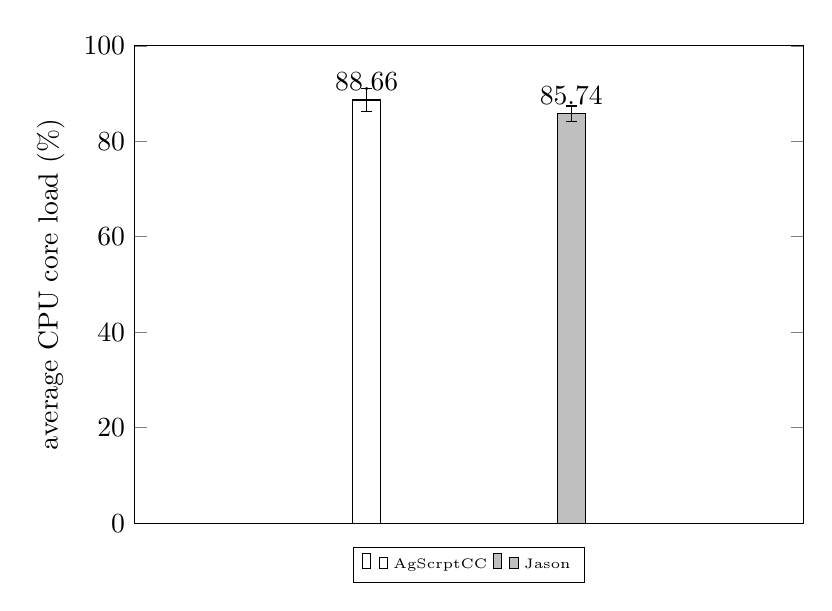
\begin{tikzpicture}
\begin{axis}[
    scale only axis,
    width=0.7\textwidth,
    height=0.5\textwidth,
    ybar,
    enlarge x limits=0.15,
    legend style={at={(0.5,-0.05),font=\tiny},
      anchor=north,legend columns=-1},
    ylabel={average CPU core load (\%)},
    xmin=-1, xmax=2,
    xtick style={draw=none},
    xticklabels={,,,},
    nodes near coords,
    nodes near coords align={vertical},
    ymin=0,
    ymax=100
    ]
\addplot[fill=black!0, error bars/.cd, y dir=both, y explicit] coordinates {(0,88.6575) +-(2.4864003978712743,2.4864003978712743)};
\addplot[fill=black!25,error bars/.cd,y dir=both,y explicit] coordinates {(1,85.73875000000001) +-(1.6477440981797706,1.6477440981797706)};

\legend{AgScrptCC,Jason}
\end{axis}
\end{tikzpicture}
     \caption{CPU load (average and standard deviation on 8 cores) in token ring with $N=4k$, $T=4k$ and $W=4k$}
    \label{fig:cpu_load_token2}
    
\end{figure}

\begin{figure}[tb!]
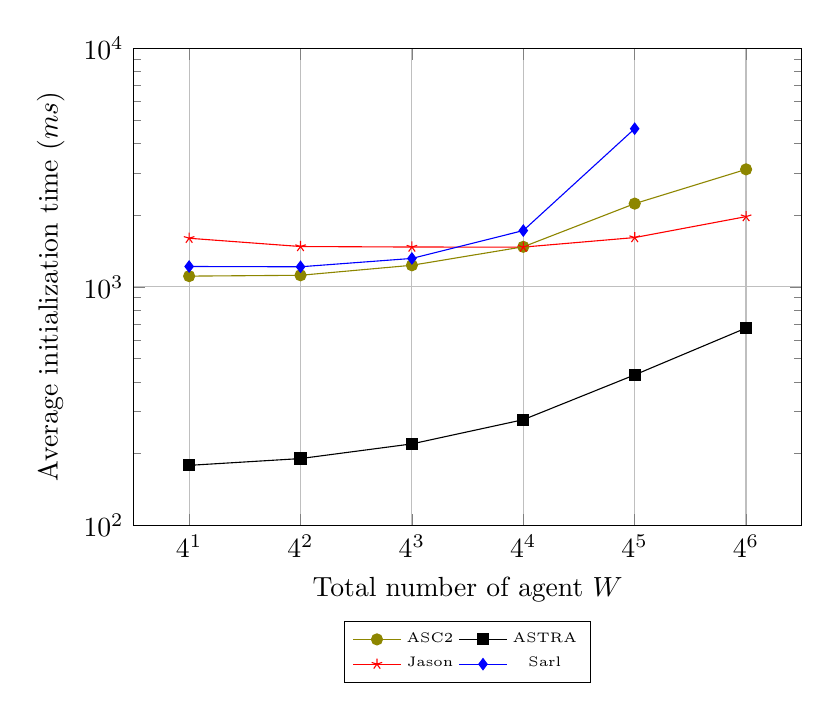
\begin{tikzpicture}
\begin{axis} [
    scale only axis,
    width=0.7\textwidth,
    height=0.5\textwidth,
    grid=major,
    transpose legend,
		legend columns=2,
		legend style={at={(0.5,-0.2)},anchor=north,font=\tiny},
    xmode=log,
    log basis x={4},
    ymode=log,
    log basis y={10},
    ymin=100,
    ymax=10000,
    xlabel={Total number of agent $W$},
    ylabel={Average initialization time ($ms$)},
    cycle list name=black white
]


    \addplot[mark=*,olive
    ]
    coordinates {
    (4 , 1108.8999999999999)
    (16 , 1118.0)
    (64 , 1231.2)
    (256 , 1471.6)
    (1024 , 2231.5)
    (4096 , 3106.0)
    };
    \addlegendentry{ASC2}
    
    \addplot[mark=star,red
    ]
    coordinates {
    (4 , 1597.7)
    (16 , 1475.5)
    (64 , 1468.2)
    (256 , 1467.1999999999998)
    (1024 , 1608.7)
    (4096 , 1969.0)
};
    \addlegendentry{Jason}
    

    
        \addplot[mark=square*,black
    ]
    coordinates {
(4 , 178.7)
(16 , 190.8)
(64 , 219.79999999999998)
(256 , 277.6)
(1024 , 427.70000000000005)
(4096 , 672.0999999999999)
        };
    \addlegendentry{ASTRA}
    
       
    \addplot[mark=diamond*,blue
    ]
    coordinates {
    (4 , 1216.7)
    (16 , 1213.6000000000001)
    (64 , 1315.3999999999999)
    (256 , 1721.2)
    (1024 , 4599.25)
    };
    \addlegendentry{Sarl}

\end{axis}
\end{tikzpicture}
\caption{Initialization time in token ring with $T=4$, $N=4$}

\label{fig:init1}
\end{figure}

\subsection{Chameneos Redux}
The second benchmark is adopted from \cite{Kaiser2003} and is a test intended to capture the effects of one limiting point to the execution framework. The scenario consists of $C$ chameneo creatures living in the jungle; they can go to a common place to meet other creatures and \textit{mutate} with them. Each creature has a color assigned to it from a color pool and after mutation its colour changes based on the color of the other creature it met. These meetings should happen for a total number of $N$ times. To run this benchmark a program should:
\begin{itemize}
    \item create $C$ differently colored (blue, red, yellow), differently named, concurrent chameneo creatures
    \item write all the possible complementary color combinations;
    \item write the initial color of each creature;
    \item each creature will repeatedly go to the meeting place and meet, or wait to meet, another chameneo;
    \item both creatures will change color to complement the color of the chameneo that they met;
    \item after $N$ meetings have taken place, for each creature write the number of creatures met and the number of times the creature met a creature with the same name (should be zero).
    \item the program finishes when $N$ meetings have happened.
\end{itemize}


The experiment was performed with the set of variables $C=\{64,256,1k,4k\}$ and $N=\{1k,4k,16k,64k\}$. This provide us with $20$ different configurations for each framework. All tests were given a $1$ minute time limit and it is considered a timeout after that.


\subsubsection{Implementation Notes} In all implementations a \textit{broker} agent is present that acts as the meeting point for chameneos. This agent is the main point of this benchmark as it will be constantly under high number of requests from the chameneos agents.

\subsubsection{Results} 

The first view on the results is presented in Figure \ref{fig:cham1}. In this setting the number of meetings $N$ is kept constant at two values $4k$ and $64k$ whilst the number of chameneos is the variable. The results show that Jason and ASC2 scale well with the number of agents while ASC2 performs marginally better in the $N=64k$ test. Sarl and ASTRA suffer from the higher number of agents to the point that Sarl could finish both tests only up to $C=1k$ agents while ASTRA finishing $N=64k$ test only in the $C=64$ agents setting.

Figure \ref{fig:cham2} presents another view on the results. This time the number of chameneos $C$ is kept constant at $256$ and $4k$, whilst the number of meetings $N$ is the variable. Sarl could only finish the $C=256$ test while ASTRA could only finish it up to $N=16k$ and timing out after that. ASTRA was also only able to finish the $C=4k$ test with $C=64$ number chameneos. ASC2 and Jason both completed the tests with linear scaling, with ASC2 outperforming Jason slightly in the $C=4k$ test. This shows that both Jason and ASC2 can handle higher levels of concurrency in the broker agent w.r.t. the increasing number of concurrent requests.

\begin{figure}[tb!]
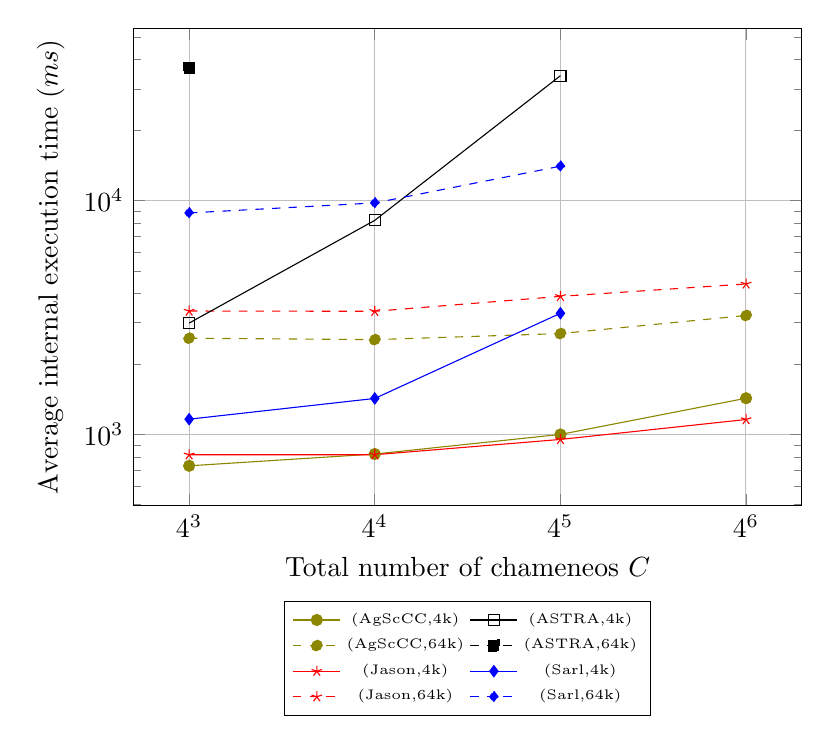
\begin{tikzpicture}
\begin{axis} [
    scale only axis,
    width=0.7\textwidth,
    height=0.5\textwidth,
    grid=major,
    transpose legend,
		legend columns=4,
		legend style={at={(0.5,-0.2)},anchor=north,font=\tiny},
    xmode=log,
    log basis x={4},
    ymode=log,
    log basis y={10},
    xlabel={Total number of chameneos $C$},
    ylabel={Average internal execution time ($ms$)},
    cycle list name=black white
]


    \addplot[mark=*,olive
    ]
    coordinates {
(64 , 733.5)
(256 , 823.8)
(1024 , 999.0)
(4096 , 1426.8)
    };
    \addlegendentry{(AgScCC,4k)}
    
\addplot[mark=*,olive,dashed
    ]
    coordinates {
    (64 , 2576.7)
(256 , 2540.6)
(1024 , 2697.0)
(4096 , 3222.8)
    };
    \addlegendentry{(AgScCC,64k)}
        \addplot[mark=star,red
    ]
 coordinates {
 (64 , 817.5)
(256 , 818.2)
(1024 , 950.9)
(4096 , 1157.2)
};
    \addlegendentry{(Jason,4k)}
    \addplot[mark=star,red,dashed
    ]
    coordinates {
(64 , 3367.3)
(256 , 3358.6)
(1024 , 3891.0)
(4096 , 4396.3)
    };
    \addlegendentry{(Jason,64k)}

        \addplot[mark=square,black
    ]
    coordinates {
(64 , 2990.9)
(256 , 8224.0)
(1024 , 34161.1)
        };
    \addlegendentry{(ASTRA,4k)}
    
    \addplot[
    mark=square*,black,dashed
    ]
    coordinates {
    (64 , 36860.8)
        };
    \addlegendentry{(ASTRA,64k)}   
    
    \addplot[mark=diamond*,blue
    ]
    coordinates {
        (64 , 1160.8)
    (256 , 1423.9)
    (1024 , 3293.9)
    };
    \addlegendentry{(Sarl,4k)}
    
    \addplot[mark=diamond*,blue,dashed]
    coordinates {
        (64 , 8846.6)
        (256 , 9760.6)
        (1024 , 14014.9)
    };
    \addlegendentry{(Sarl,64k)}
    


\end{axis}
\end{tikzpicture}
\caption{Chameneos redux results for each (framework, $N$)}

\label{fig:cham1}
\end{figure}

\begin{figure}[tb!]
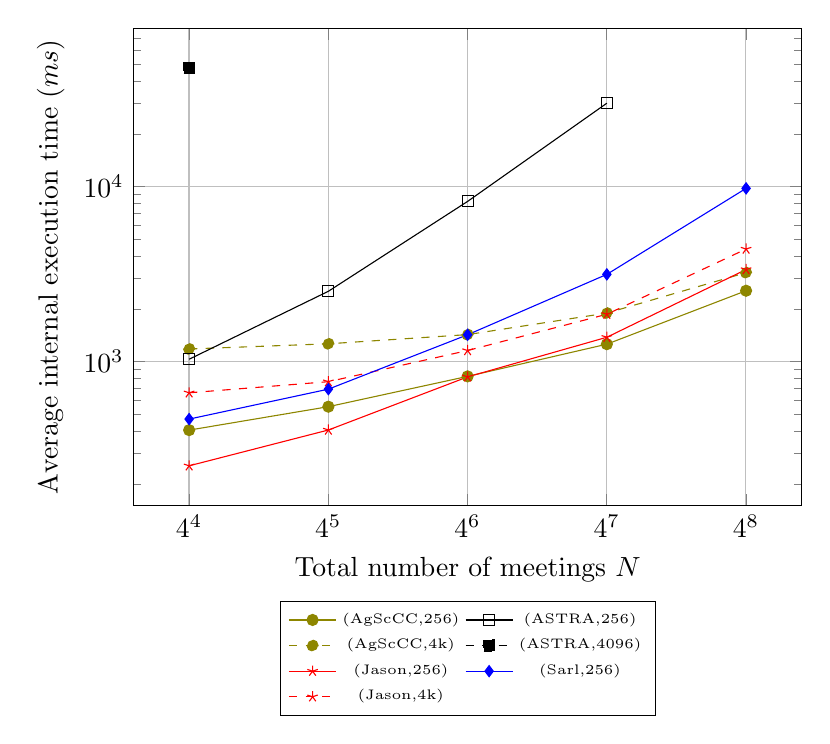
\begin{tikzpicture}
\begin{axis} [
scale only axis,
    width=0.7\textwidth,
    height=0.5\textwidth,
    grid=major,
    transpose legend,
		legend columns=4,
		legend style={at={(0.5,-0.2)},anchor=north,font=\tiny},
    xmode=log,
    log basis x={4},
    ymode=log,
    log basis y={10},
    xlabel={Total number of meetings $N$},
    ylabel={Average internal execution time ($ms$)},
    cycle list name=black white
]

\addplot[mark=*,olive
    ]
    coordinates {
(256 , 406.3)
(1024 , 552.9)
(4096 , 823.8)
(16384 , 1258.0)
(65536 , 2540.6)
    };
    \addlegendentry{(AgScCC,256)}
    
    \addplot[mark=*,olive,dashed
    ]
    coordinates {
(256 , 1180.9)
(1024 , 1264.3)
(4096 , 1426.8)
(16384 , 1893.3)
(65536 , 3222.8)
    };
    \addlegendentry{(AgScCC,4k)}
    \addplot[mark=star,red
    ]
    coordinates {
(256 , 254.1)
(1024 , 406.9)
(4096 , 818.2)
(16384 , 1377.9)
(65536 , 3358.6)
    };
    \addlegendentry{(Jason,256)}
    \addplot[mark=star,red,dashed
    ]
 coordinates {
(256 , 663.7)
(1024 , 768.3)
(4096 , 1157.2)
(16384 , 1864.9)
(65536 , 4396.3)
};
    \addlegendentry{(Jason,4k)}
    
    \addplot[mark=square,black
    ]
    coordinates {
(256 , 1031.8)
(1024 , 2522.3)
(4096 , 8224.0)
(16384 , 29916.6)
        };
    \addlegendentry{(ASTRA,256)}
    
        \addplot[mark=square*,black,dashed
    ]
    coordinates {
(256 , 47535.6)
        };
    \addlegendentry{(ASTRA,4096)}
    
       
    \addplot[mark=diamond*,blue
    ]
    coordinates {
    (256 , 469.7)
(1024 , 696.3)
(4096 , 1423.9)
(16384 , 3150.7)
(65536 , 9760.6)
    };
    \addlegendentry{(Sarl,256)}

   \addplot[mark=diamond*,blue]
    coordinates {

    };
    \addlegendentry{(Sarl,4096)}

\end{axis}
\end{tikzpicture}
\caption{Chameneos redux results for each (framework,$C$)}

\label{fig:cham2}
\end{figure}



\subsection{Service Point}
This last benchmark is not about performance. Rather, it is designed to illustrate the differences between the execution in a \textit{step-based} framework like Jason in contrast to a compilation-based framework like ASC2, focusing on how they handle actions (namely time-consuming primitive actions) specified outside their DSL. The scenario of this benchmark consists of one service point and $N$ number of consumers. Each consumer sends $R$ requests to the service point and waits for the response. The service point needs a random  amount of time $t$ ($0 \le t \le 5000$ ms) to process each request. A simple \verb+Thread.sleep(t)+ is used to mimic thread time consumption. To run this benchmark a program should
\begin{itemize}
    \item create $1$ service point and $N$ service consumers.
    \item each consumer will send $R$ number of requests to the service point
    \item the program finishes when all of the $R*N$ requests have been responded 
\end{itemize}
The experiment was done only on Jason and ASC2 with variables $N=\{1,4,16\}$ and $R=\{1,4,16\}$. With respect to total number of request $R*N$, this gives us with 5 unique configurations. To account for the non-determinism added by the randomization each configuration is executed for $100$ times.

\subsubsection{Results}
The results of this experiment are presented in Figure \ref{fig:ping_pong1}. Jason performs much worse in this scenario, as it is not being able to finish the $256$ requests within a $200$ seconds timeout. This is even more strange as in our setting Jason is set to use $8$ threads and ASC2 to $6$ and by looking at the results we can see that ASC2 is always using the thread times completely but Jason is not. The reason for this is that Jason uses a \textit{sequential} reasoning cycle inside each agent; %in a symbolic way; 
at every reasoning cycle, a Jason agent takes the next step from each of its intentions and executes them. The reasoning cycle ends when all intentions execute one step. This means that if in the reasoning cycle of an agent one of these steps is a time-consuming primitive action, the whole cycle will be blocked\footnote{Jason provides extra built-in directives like \texttt{.wait} to mimic unblocking suspension of intentions but that is beyond the context of this benchmark.}. On the contrary a compiled agent does not have any notion of steps at run-time and the parallelism between intentions of the agent is also handled by the underlying concurrency model, in this case the Actor model. This matter is further discussed in \ref{subsec:par}.

\begin{figure}[bt!]
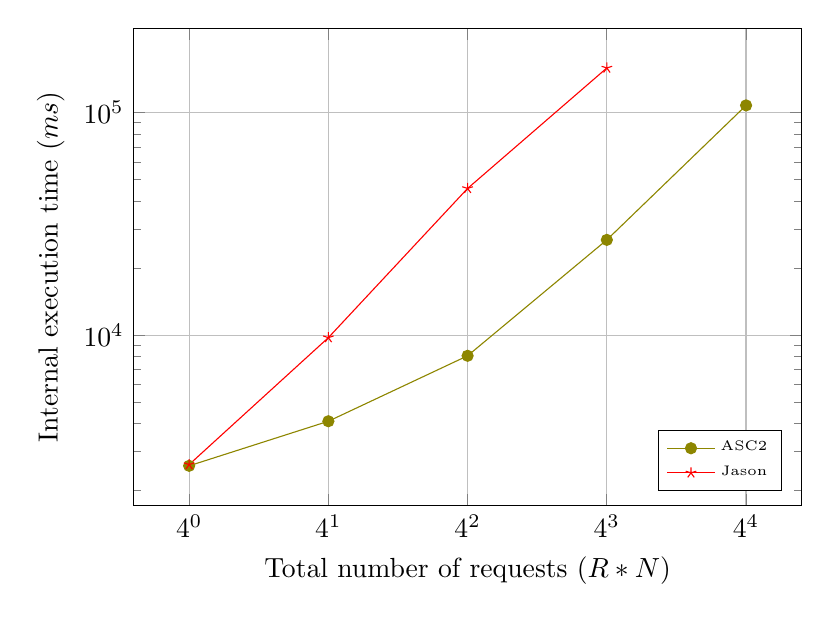
\begin{tikzpicture}
\begin{axis} [
    scale only axis,
    width=0.7\textwidth,
    height=0.5\textwidth,
    grid=major,
    legend pos=south east,
    legend style = {font=\tiny},
    xmode=log,
    log basis x={4},
    ymode=log,
    log basis y={10},
    xlabel={Total number of requests ($R*N$)},
    ylabel={Internal execution time ($ms$)},
    cycle list name=black white
]
\addplot[mark=*,olive
    ]
    coordinates {
    (1,2586.46)(4,4101.450000000001)(16,8072.993333333333)(64,26780.0)(256,107672.52)
    };
    \addlegendentry{ASC2}
    \addplot[mark=star,red
    ]
    coordinates {
    (1,2619.74)(4,9738.456756756757)(16,45602)(64,158538)
    };
    \addlegendentry{Jason}
\end{axis}
\end{tikzpicture}
\caption{Service point scenario results}
\label{fig:ping_pong1}
\end{figure}

\section{Discussion}
\label{sec:discussion}
This chapter presents and evaluates a framework for an AOP language based on AgentSpeack(L) relying on compilation. Compilation in this context is not novel as it has been used previously by other AOP frameworks like SARL \cite{Sarl} and ASTRA \cite{Astra}. The novelty of this work lies in two aspects. First, unlike SARL and ASTRA, that use a DSL very close to their underlying language (Java), ASC2 uses a logic-based DSL close to AgentSpeak(L). %\Gio{but in principle,} 
As our pipeline starts from an \textit{antlr} grammar, in principle 
the current DSL can be replaced by any other AOP language that can be mapped to the ASC2 abstract execution architecture. Second, our approach maps the DSL into an architecture that exploits the Actor model. This means that not only the final executable model is more robust, because it takes advantage of the established concurrency model and the maturity of the libraries implementing the Actor model (e.g, Akka), but also that the translation itself is an open process, so its product becomes in principle more understandable for the programmer.


\subsection{Performance}
The execution model of ASC2 is closer to Sarl and ASTRA than to Jason (see \ref{subsec:par}), but, as shown by the benchmarks, it is substantially outperforming both Sarl and ASTRA. At the same time, ASC2 performance was below what we expected before running these experiments. Investigating possible causes by profiling the execution of benchmarks, we found out that a considerable amount of execution time is spent on the blocking due to \textit{synchronized query calls} to the belief base. These calls had to be synchronized because Prolog engines like \textit{Styla} and \textit{tuProlog} \cite{tuprolog} (another candidate solution we tested for handling belief bases) are inherently made for single thread access. Even a simple \textit{read} query to a Prolog engine still counts as \textit{write} access because of the backtracking.
%Interestingly enough Jason does not have any issue with this because, as presented in \ref{subsec:par}, the intentions of one Jason agent are only symbolically concurrent, therefore there will be no need to synchronize belief base access as they are ultimately sequential. 
We believe once this issue is addressed the performances of ASC2 will greatly improve.


\subsection{Language}

Although all of the considered frameworks propose DSLs to program reactive agents, their bases are different. %the ideas behind them differ.
Agent-ScriptCC's DSL is based on AgentSpeak(L), which gives to the language a logic-oriented flavour; this is also the case for Jason, and both frameworks can take advantage of Prolog-style terms and expressions. ASTRA's DSL is also based on concepts defined in AgentSpeak(L) but with more syntactic resemblance to Java. Sarl's language does not try to be a logic-based language, therefore it does not contain components corresponding to terms or expressions; it is rather very close to Java.

% Noone asked!
%\subsubsection{Type system}
%The desirability of a language to be typed depends on the application it is used for. Among these frameworks Jason and ASC2 are un-typed while ASTRA and Sarl are typed.% Note that Sarl allows for shared declaration of event types but in ASTRA programs, every formula needs to be introduced as a type in each agent program.

\subsection{Execution and Parallelism}
\label{subsec:par}
As a common ground, all these frameworks are used to specify reactive agents, but they differ in how the agent's (re)actions are executed. The most particular solution comes with Jason which uses the concept of \textit{steps}. The Jason interpreter treats each symbolic step/instruction in a plan of a reactive rule as a single unit of execution, and emulates an imperative program by executing them in a sequence in consecutive reasoning cycles. In contrast, in the other three frameworks, the steps of the reactive rules are already imperative programs ready to be executed. The approach taken by Jason has important consequences especially when agents execute multiple parallel threads of work (intentions) at the same time. This concept is examined more in detail in section \ref{sec_bench} and in \cite{Astra}.

\subsection{Access to the Lower-Level Language}
One of the motivations behind developing ASC2 has been to enable access to libraries defined in the underlying general-purpose programming language of choice in a easy and seamless way. In our view this impacts the usability of the framework in larger applications. Leading by an example, consider a programmer that needs to call the Java function \verb+Thread.sleep(1)+ in a reactive rule. In Jason one needs to create an extra class extending one of Jason's internal classes (\verb+Agent+, \verb+Action+ or \verb+Environment+) and define a method that wraps this low level function and then call the wrapping method from the agent program. In ASTRA it is almost the same as Jason and one needs to create a class extending the type \verb+Module+, wrap this function inside a method, and annotate it appropriately to be able to call it from the agent program. On the opposite side, this is entirely different for Sarl and ASC2, as one can simply call this function directly from the agent program. In case of ASC2 this can be done with \verb+#Thread.sleep(1)+.

\subsection{Communication}
The communication in ASC2 is entirely externalized, both for agent-to-agent and agent-to-environment communication. In the current implementation communication between agents uses Akka's internal message system but this can easily be replaced with any other type of communication mechanism, e.g. by using a message queue (\textit{MQ}) to be able to execute the agents in a distributed setting. For the other frameworks, externalization is possible, but requires specific wrappers to the communication infrastructures (Jason with JADE).

\section{Conclusion and Future developments}
%The slowly but steadily increasing interest in languages based on BDI or functionally similar architectures for virtual assistants, robotics, (serious) gaming, as well as for social simulations, hints that there is a general consensus that these solutions might be suitable to reproduce human-like reasoning, or rather human-intelligible computation. So far, the majority of contributions in this area were concerned mostly by the logical aspects of the problem rather than its computational aspects \cite{Herzig2017}. Indeed, intentional (or alternatively \textit{policy-based}, or also \textit{purpose-driven}) programming (dealing with why) aims to provide a different level of abstraction w.r.t. declarative programming (dealing with what, or the outcome) and imperative programming (dealing with how, or operations), and understanding its specificities and identifying sound logical properties are crucial passages. 

The slowly but steadily increasing interest in programming languages based on BDI or functionally similar architectures for virtual assistants, robotics, (serious) gaming, as well as for social simulations, hints that there is a general consensus that these solutions might be suitable to reproduce human-like reasoning, or rather human-intelligible computation. 

Historically, the majority of contributions in this area were concerned mostly by the logical aspects of the problem rather than its computational aspects \cite{Herzig2017}. However, more recent contributions %made clear the presence of relevant 
revealed the presence of issues w.r.t. computational performance and compatibility to modern environments and tools, motivating efforts to redevelop existing BDI frameworks according to best practices \cite{LJ,pyson}. Looking at intentional programming in the longer term, we need to acknowledge that operational settings differ from the typical low-scale simulation setting in which it is used today. Besides a difference in scale, components can also be fully distributed. %, and time synchronization cannot be guaranteed (or at least only to a certain extent). 
Because of this, a future target feature of ASC2 will be the capability to deploy and execute agents in distributed settings. This seems to be an achievable objective as there are already approaches available to run actors in distributed environments.% Another related concept to be investigated, both at theoretical and practical levels, is to extend event-based reactivity of the agents into stream-based reactivity, to enable agent programs to be used for modern data-centric applications.

An initial, additional motivation of using an actor-oriented architecture for the intentional agents is that by having this extra level of abstraction the agent become more modular, enabling the augmentation of agents with complementary machinery like using AI modules \cite{Singh2011IntegratingLI}, normative reasoning modules \cite{meneguzzi2009norm}, planning (e.g. HTN, STRIPS) modules \cite{meneguzzi_de_silva_2015} and preference checking modules \cite{Visser2016,Mohajeri2019}. Defining  adequate interfaces to support the different types of add-ons for ASC2 agents will be investigated in the future.

The present work acts as a starting block towards this path. The benchmarks reported here demonstrates that, despite the initial maturity level of the framework, ASC2 is already competitive against existing frameworks, motivating further exploration.

%Furthermore, agents might encapsulate other AI modules (e.g. machine learning-based) that are better executed if concurrency is safe. % This abstraction level is relevant also because purpose is one of the elements that enable to recognise e.g. legitimate processing (e.g. according to GDPR). Most applications in this area introduce purpose only as meta-data of requests, and in doing so they break the connection between performance and (intended) outcome. In principle, recovering this link would facilitate the maintenance of applications as well as the social functioning of the infrastructure.

%Furthermore, we believe there are still mechanisms to be explored at intentional level of agents, e.g, addressing the gap between goals and desires \cite{Dignum2002} or having explicit preferences as part of the script \cite{Mohajeri2019}.
 %(e.g. agent's desires are for the most considered only in the reduced form of goals)
 %we decided to follow a different path than building from scratch yet another framework. We decided instead to experiment with the reuse of established, robust components as actors. 
% By approaching an intentional agent as a system of actors, %designers are enabled
 %we can test different theories in a more structured way by mapping them to externally programmable strategies for the actor-based architecture, %: even if these actors are functionally constrained by 
 %either by recomposing the abstract architecture or by restructuring the interactions between (agent-internal) actors.
 
 %Second, by establishing a direct mapping of the scripts to the underlying language, programmers can enjoy of a direct connection with existing ecologies of tools such as debuggers, profilers, build tools, etc. an option that in principle facilitates adoption. The partial success of ASC2---still at its infancy---on the various benchmarks investigated here confirms us that this might be a viable path.

\chapter{Transparent Decisions in Social Actors: Preferences}
\label{ch:preferences}
Computational agents based on the BDI framework typically rely on abstract plans and plan refinement to reach a degree of autonomy in dynamic environments: agents are provided with the 
ability to select \textit{how-to} achieve their goals by choosing from a set of options. In this work we focus on a related, yet under-studied feature: \textit{abstract goals}. These constructs refer to the ability of agents to adopt goals that are not fully grounded at the moment of invocation, refining them only when and where needed: the ability to select \textit{what-to} (concretely) achieve at run-time. We present a preference-based approach to goal refinement,  defining preferences based on extended \textit{Ceteris Paribus} Networks (CP-Nets) for an AgentSpeak(L)-like agent programming language, and mapping the established CP-Nets logic and algorithms to guide the goal refinement step. As a technical contribution, we present an implementation of this method that solely uses a Prolog-like inference engine of the agent's belief-base to reason about preferences, thus minimally affecting the decision-making mechanisms hard-coded in the agent framework. The aim of this chapter is to (1) introduce a generic approach for embedding explicit preferences into BDI agents, and (2) to provide a proof-of-concept implementation of this approach in ASC2. 


\section{Introduction}
% \Mos{It's not CP-Nets any more, mostly it's CP-Theories, need to change some text}

%new_commnent As computational agents intervene more and more in human activities, there is an increasing demand for human-oriented forms of programming, i.e. relying on concepts and abstractions mapping intuitively to what humans utilize to explain and direct their behaviour. The \textit{belief-desire-intention} (BDI) model of agency \cite{Rao1995}, centred around a general theory of mind \cite{bratman1987intention}, offers one of those views, and has been studied by the community since the 90s, resulting in the proposal and development of several platforms for agent-based programming (e.g. AgentSpeak(L)/Jason \cite{RaoAS1996,Bordini2005}, 3APL/2APL \cite{Dastani2APL}, GOAL \cite{Hindriks2009a}, IMPACT \cite{IMPACT}, JACK \cite{JACK}, Astra \cite{ASTRA}, LightJason \cite{Aschermann2018}, ASC2 \cite{mohajeriparizi_2020_run}---a  systematic review of logic-based MAS frameworks can be found in \cite{MASReview2021}).

Computational agents based on the BDI framework typically rely on abstract plans and plan refinement to reach a degree of autonomy in dynamic environments. In practice, relative autonomy in this context consists in the ability of an agent to select \textit{how-to} achieve their goals by choosing from a set of options. BDI agent scripts typically consist of hierarchical, partial, abstract plans. This contrasts with classic forms of planning, providing agents with fully-grounded policy, designed to reach a certain specific objective. 

This work focuses on a related, yet under-studied feature: % present in BDI frameworks, particularly in those based on the AgentSpeak(L) language:
%(although already present in frameworks as those based on the AgentSpeak(L) language)
\textit{abstract goals}. These constructs refer to the ability of agents to adopt goals that are not fully grounded at the moment of invocation, refining them only when and where needed, that is, the ability to select \textit{what-to} (concretely) achieve at run-time. Examples of abstract goals can be found typically in \textit{activity}-level characterizations of behaviour, e.g. walking (where?), eating something (what?), meeting someone (who?), selling (what? to whom?), etc. 

The specification of abstract goals is a feature already present in some agent frameworks as those based on the AgentSpeak(L) language, albeit they rely on simplistic mechanisms for goal refinement. The present work aims to cover the goal refinement step (from abstract goals to concrete goals) as part of the agent's decision-making cycle. For doing so, 
we present a preference-based approach to goal refinement. We start from defining preferences based on \textit{Ceteris Paribus} Networks (CP-Nets) \cite{Boutilier2004}---more precisely, in the extended form of \textit{Ceteris Paribus} Theories (CP-Theories) \cite{Wilson2004}---and we consider the established CP-Net logic and algorithms to guide the goal refinement of the agent. At implementation level, our target is an AgentSpeak(L)-like \cite{RaoAS1996} agent programming language. Since Jason \cite{Bordini2005},  AgentSpeak(L) programs are enriched with Prolog rules and facts for knowledge-level processing, occurring e.g. for testing context conditions during the plan selection phase. We present therefore an implementation of a preference-based goal refinement method that solely uses a Prolog-like inference engine of the agent's belief-base to reason about preferences, requiring only a minimal modification to the decision-making mechanisms hard-coded in the agent framework. To achieve this, a transformation method is proposed to map an extended version of CP-Nets and CP-Theories into Prolog facts and rules for the script of the AgentSpeak(L) agent, as well as a Prolog implementation of the algorithms necessary to reason with preferences.

The chapter proceeds as follows: section \ref{sec:2} provides a background about the concepts used in this work; section \ref{sec:method} presents the method and examples for preference-based abstract goal refinement in AgentSpeak(L) agents; section \ref{sec:implementation} describes a practical implementation of this method, and section \ref{sec:discuss} elaborates a discussion and conclusion over the proposed method. 

% \begin{comment}

% [Copied]

% In the last decades several attempts have been made to move from machine-oriented views of programming towards concepts and abstractions that more closely reflect the way in which humans conceive the world. In particular, the \textit{belief-desire-intention} framework (BDI) \cite{Rao1995}, building upon a theory of mind \cite{bratman1987intention}, has been introduced to provide a basis for the implementation of computational agents that exhibit rational behaviour, using the same representations that we typically use to address human behaviour. % Additionally, from a modeling  standpoint, the BDI framework offers a cognitive model for agent-based modelling (ABM) \cite{balke2014}, 
% %\subsubsection{Why prioritize BDI scripts with preferences}
% In the %related 
% decision-making literature, instead, particular attention is given to the role of preferences: any model of agency involving decision-making is deemed to abide the agent's preferences \cite{Pigozzi2016}. This does not imply that any model of agency will rely on explicit preferences, rather it affirms the general principle that when there are multiple goals that should be achieved (or multiple ways to achieve a certain goal or even multiple sets of states that can be reached) the best course of action is the one that abides the most to the agent's preferences \cite{Pigozzi2016}.
% In practice, preferences can vary from the implicit ``maximize utility" of optimizing agents \cite{Nunes2014} to explicit preferences specified in a preference representation language \cite{Dasgupta2010,Visser2011}. 
% % BDI agent execution architectures, more often than not, rely on logical constructs for modeling the agents' mental components, see e.g. the critical overview given in \cite{Herzig2018}. 
% %Unexpectedly, none of the main BDI languages presented in the literature support explicit preferences. %Decisions between alternative choices (in our case, for plan selection) are generally based on implicit forms of preferences like sequential ordering (e.g. of plan specifications).% Only a few works have investigated a potential role for explicit preferences in BDI agents \cite{Dasgupta2010,Visser2011,Nunes2014,Mohajeri2019}

% \end{comment} 

%%%%%%%%%%%%%%%%%%%%%%%%%%%%%%%%%%%%%%%%%%%%%%%%%%%%%%%%%%%%%%%%%%%%%%%%

\section{Background} 
\label{sec:2}
%\Mos{we need to make a choice (later) to keep the related works here or move them to discussion. Some like GAI networks or other preference frameworks do not make much sense in discussion, but other BDI/Pref ones do for comparison} 
% This section provides an overview of the concepts and methods on which our contribution builds upon. Most of these sections are succinct version of what presented in \cite{Mohajeri2019}.
% \vspace{0pt} \noindent \textbf{BDI Agents} \quad
\subsection{Abstract Plans in BDI Agents}

Agents specified following the BDI paradigm are characterized by three mental attitudes. Beliefs are facts that the agent believes to be true. Desires capture the motivational dimension of the agent, typically conflated with the more concrete form of \textit{goals}, representing procedures/states that the agent wants to perform/achieve. Intentions are selected conducts (or \textit{plans}) that the agent commits to (in order to advance its desires). 

Since their origin \cite{Rao1995}, the essential feature associated to BDI architectures is the ability to instantiate abstract plans that can (a) react to specific situations, and (b) be invoked based on their purpose. Consequently, the BDI execution model often relies on a \textit{reactive} model of computation, usually in the form of some type of \textit{event-condition-action} (ECA) rules often referred to as \textit{plans}. Plans are uninstantiated specifications of the \textit{means} (in terms of course of actions) for achieving a certain \textit{goal} \cite{Rao1995}. These constructs represent the procedural knowledge (\textit{how-to}) of the agent. There are multiple proposals in the literature for programming language and architecture of BDI agents, the most commonly used being AgentSpeak(L) \cite{RaoAS1996}, which will serve as basis for the present proposal. % is also based upon the AgentSpeak(L) language and a more detailed description of it is presented in section \ref{ssec:agentspeak}.

%\vspace{5pt} \noindent \textbf{Preferences in BDI agents} \quad
% Multiple BDI languages and frameworks have been introduced in the literature, typically in form of \textit{Multi-Agent System (MAS)} frameworks, such as AgentSpeak(L)/Jason \cite{RaoAS1996,Bordini2005}, 3APL/2APL \cite{Dastani2APL}, GOAL \cite{Hindriks2009a}, IMPACT \cite{IMPACT}, JACK \cite{JACK}, Astra \cite{ASTRA}, LightJason \cite{Aschermann2018}, and ASC2 \cite{mohajeriparizi_2020_run}. 

%All of these frameworks  In current BDI implementations, preferences between these optional conducts are specified through a static ordering assigned by the programmer, typically via the ordering of rules in the code: the higher a rule is in the script, the more priority the associated plan has. 

%This explains why most current frameworks including Jason \cite{Bordini2005}, 2APL \cite{Dastani2007}, ASC2 \cite{mohajeriparizi_2020_run}, etc. are genuinely \textit{reactive}: the scripts are interpreted without the need for any additional introspection/deliberation steps. However, these frameworks also expose \textit{plan selection} functions that can be modified to implement alternative mechanism for goal-plan rule selection during the deliberation cycle which can be considered as a type of meta-programming over agent scripts. % As it was said before, this approach has the positive features of simplicity, readability and performance while having the issue that these order-based preferences stay in the mind of programmer, and are not represented as explicit preferential knowledge.
% For more clarity, to better separate goal-adoption from the treatment of primitive actions, we will not consider primitive actions as part of preferences. 
%[???] 
%The latter option has been taken by almost all works adding explicit preferences to BDI agents \cite{Visser2011,Dasgupta2010,Nunes2014}: the selection of the most preferred alternative is taken as a \textit{reflective} process, where preferences provide a \textit{rationale} to be applied online during the agent's deliberation cycle.  The idea of relying on an offline step is instead proposed also in \cite{Mohajeri2019}, but they only focused on \textit{procedural preferences} (``I prefer to be doing $a_i$ rather than doing $a_j$"), which have a different level of abstraction w.r.t. to declarative preferences (``I prefer being in state $s_i$ rather than being in state $s_j$"). % This chapter focused instead on \textit{declarative preferences}, i.e. about states of the world (``I prefer being in state $s_i$ rather than being in state $s_j$"). For this purpose, we used the notions of (1) \textit{declarative goals} (``want-to-be'' goals), and of (2) \textit{post-condition} or effect specification of \textit{primitive actions}. 
%Modifying the deliberation cycle by adding run-time reflective steps (as a complex preference checking and related plan selection algorithms) is generally detrimental to reactivity

%$\paragraph{Reasoning cycle}

%There is an extensive literature between BDI agent programs and HTNs (\textit{hierarchical task networks}) planning domains \cite{DeSilva2019,Meneguzzi2013}.
%Solutions to classic planning problems are concrete sequence of actions, to be performed by the agent to reach a certain goal. 
%Plan refinement \cite{Kambhampati1997} considers the set of all action sequences and manipulates it progressively following diverse strategies, narrowing it down to the set of possible solutions. The manipulation occurs via partial plans, which for this reason can be seen as behavioural constraints. % Yet, planning approaches typically do not consider abstraction of actions  \cite{Hoffmann2006}, nor of goals.
%Rather than looking at all solutions, and then evaluating those to select the best one, the decision-making cycle of reactive BDI agents---as those specified in AgentSpeak(L)---selects the first available plan. From this point of view, they can be seen as ``reactive planning systems'' \cite{Wooldridge1995a}. However, differently from planning systems, BDI agents do not form a complete solution up-front, but unveil it on the fly, so it may happen that, given a problem, a solution is partially formed, partially executed, when an external event changes the search towards another problem.


%\Gio{[Here there should be more detail about the decision-making cycle used in AgentScript, so that people understand why the Prolog mechanism is fine as a solution.]}
%\Mos{moved to 3.1, so we can focus on AgentSpeak}

%\vspace{5pt} \noindent \textbf{Preference languages} \quad

\subsection{Preference Languages}
Preferences play a crucial role in decision-making \cite{Pigozzi2016}. Several models of preferences have been presented in the literature (e.g. on decision-making, planning, etc.), with various levels of granularity and expressiveness (see e.g. \cite{Domshlak2011}). Several models of preferences have been presented in the computational literature, with various levels of granularity and expressiveness. For a comprehensive overview (specifically in AI planning), we direct the reader to \cite{Baier2008,Brafman2009}. On a higher level, preference representation methods can be divided into \textit{quantitative} and \textit{qualitative} \cite{Baier2008}.

The most straightforward \textit{quantitative} approaches are based upon \textit{utility theory} and related forms of decision theory.% under which both planning and action selection problems are shown to be effectively expressed. %, either in deterministic or non-deterministic environments. 
Typically, in quantitative approaches there is a utility function that assigns to each action in each state a (negative or positive) value, then the agent/the planner system tries to \textit{maximise} its utility by choosing actions that would result in higher total utility (including avoiding actions with negative utility, e.g. due to cost). 

A hybrid quantitative method is provided by PDDL3 \cite{Gerevini2005}, an extension of the \textit{planning domain definition language} (PDDL) \cite{McDermott1998}. Although based on qualitative descriptions, these preferences are considered quantitative \cite{Baier2007} because the valuation of each preference is expressed with a numerical value.
%In \cite{Cranefield2017} one can find some examples of integration of these types of preferences in a BDI architecture.
Although utility-based approaches bring clear computational advantages, they also suffer from the non-trivial issue of translating users' preferences into utility functions. 

%This explains the existence of a family of \textit{qualitative} or hybrid solutions. A hybrid method is provided by PDDL3 \cite{Gerevini2005}, an extension of the \textit{planning domain definition language} (PDDL) \cite{McDermott1998}.% Although based on qualitative descriptions, these preferences are considered quantitative \cite{Baier2007} because the valuation of each preference is expressed with a numerical value.
%, as LPP \cite{Bienvenu2006} and PDDL3 \cite{Gerevini2005}. 

This explains the existence of a family of \textit{qualitative} or hybrid solutions. % that allow for explicit specification of preferences. 
The \textit{logical preference description} (LPD) language \cite{Brewka2004} uses ranked knowledge bases alongside preference strategies to present preference descriptions. The LPP language \cite{Bienvenu2006} is a first-order preference language defined in situation calculus to reason about conditional and qualitative preference.
%Proposals exist for integrating LPP in BDI agents \cite{Visser2011}. 
Other preference models, such as GAI networks \cite{Gonzales2004}, CP-Nets \cite{Boutilier2004} and qualitative preference systems (QPS) \cite{Visser2012QPS}, have been specifically introduced for taking into account dependencies and conditions between preferences. GAI networks build upon the assumption of \textit{generalized additive independence}, and in doing so they enable computing the utility contribution of every single attribute/subset of attributes. QPS offers a framework for representing multi-criteria preferences based on a lexicographic rule which combines basic preferences over variables, and a cardinality-based rule which counts criteria that are satisfied; QPS have been extended with goal-based preferences \cite{Visser2013QPS}, allowing to define preferences from the context of goals.

% Whereas CP-nets have weak constraints,  (they can be seen as the preferential counterpart of Bayesian networks). CP-nets and GAI-networks share possibility to be illustrated as intuitive graphical models. 
In the present work, we decided to focus on CP-Nets, and their extension CP-Theories \cite{Wilson2004}, for two main reasons: they rely on weaker assumptions, and exhibit primarily a qualitative nature. 

%To our knowledge, \cite{Mohajeri2019} was the first attempt to introduce this type of representational models in a BDI architecture, although focusing only on procedural preferences.
%This work continues the previous effort by considering declarative preferences.

\subsubsection*{Ceteris Paribus networks (CP-Nets) }
Conditional \textit{ceteris paribus}  preferences networks (CP-Nets) are a compact representation of preferences in domains with finite \textit{attributes of interest} \cite{Boutilier2004}. An attribute of interest is an attribute in the world (e.g. \textit{restaurant}) that the agent has some sort of preference over its possible values (e.g. \textit{italian} and \textit{french}). CP-Nets build upon the idea that most of the preferences people make explicit are expressed jointly with an implicit \textit{ceteris paribus} (``all things being equal'') assumption. For instance, when someone says ``I prefer a French restaurant over an Italian one'', they do not mean at all costs and situations, but that they prefer a French restaurant (over an Italian one), all other things being equal. An example of \textit{conditional preference} is ``If I'm at a French restaurant, I prefer fish over meat''.
CP-Theories \cite{Wilson2004} extend CP-Nets adding stronger conditional statements with the construct ``\textit{regardless of}'', allowing some attributes to be released from the equality rule. 

In general, CP-Nets can be associated with two tasks: (1) finding the most preferred outcome on a certain domain of variables (2) comparing two outcomes with different criteria. Both CP-Nets and CP-Theories provide efficient algorithms for these tasks.

%\Gio{[I would introduce here more about the formalism]}
%\Gio{[Which are the typical inferences to be performed on CP-nets? Which are the tools? complexity?]}

\subsubsection{Preferences in BDI Agents}
Goals are used to identify desired states or outcomes, and preferences are used to identify more (or less) desired states or outcomes. While goals are a central aspect in BDI agents, so far, none of the main BDI frameworks and languages include preferences as part of the definition of the agents. This explains why there exist already previous studies that, like this work, attempt to  enhance BDI agents with explicit preferences. Visser et al. \cite{Visser2011,Visser2016} present an approach to embed preferences defined in the LPP language into BDI agents to guide plan selection. Nodes in the goal-plan tree of the agent are annotated by the designer about the effects of that plan and then this information is propagated automatically to other nodes in the tree at compile time. Then, at run-time, the agent uses the LPP logic to select the most preferred plan for a goal based on this information. 
Dasgupta et al. \cite{Dasgupta2010} proposes a lookahead method to enhance AgentSpeak(L) agents with constraints and objectives that the agent can use for plan selection at run-time; their approach also requires annotations for plans to reason about the preferability of plans. Mohajeri et al. \cite{Mohajeri2019,Mohajeri2020} add preferences in form of CP-Nets in AgentSpeak(L)-like agents, however, their approach consider a cross-compilation step: %that creates a conditional ordering over the plans of the agent. %with respect to a set of preferences. 
they annotate primitive actions of agents with their expected effects, and this information is then propagated through the goal plan tree to create a conditional ordering between plans. Padgham et al. \cite{Padgham2013} add situational preferences as part of plan definitions in a BDI language. The agent can use them to quantify the value of each plan at run-time. Their method is similar to this work in the sense that it does not require any lookahead, but it is different because they add preference valuations as part of each plan, which are then used in plan selection with the implicit preference of maximizing them---this makes the approach essentially a quantitative one.

%\subsection{Autonomy
%\Gio{[Perhaps something should be here about what we mean as autonomy {or perhaps this is good for the conclusion}.]}
%\Mos{Giovanni can write this}

% As this work is an initial step in integrating preferences in BDI scripts the full power of CP-nets and its extensions is not utilized yet. % the point here is to show as a proof of concept how such compact presentation can be used in this manner.
%An attribute $A$ is said to be the parent of attribute $B$ if preferences over $B$ are conditional over values of $A$. 


\section{Method}
 \label{sec:method}
% \color{lightgray}
% Highlight Points:
% \begin{itemize}
%     \item Explicit Preferences
%     \item CP-nets
%     \item preferability vs. applicability
%     \item Comparing our CP-net with original
%     \item Preferences are written in Logic form
%     \item Reasoning only happens inside agent's belief base / minimal extra machinery
% \end{itemize}

\subsection{AgentSpeak(L) Agents}
\label{ssec:agentspeak}
While this work mainly focuses on ASC2 as the BDI framework, the methods proposed in this chapter target any frameworks that utilize AgentSpeak(L). The main point of interest in BDI reasoning cycle for the preference reasoning approach proposed in this chapter is the plan instantiation process. This process, as it was briefly introduced in the previous section, starts when an event is selected for processing. Firstly the event is unified with the triggering events of the plans in the plan library. The ones that do unify are called relevant plans and the resulting unifier is called the relevant unifiers. Then, for each relevant plan, the relevant unifier is applied to its context condition and the result is queried against the belief base to create zero or more substitutions such that the context is a logical consequence of agent's current belief. The composition of relevant unifier with each substitution is called an \textit{applicable unifier}.  The following definitions apply:


% Based on the definitions proposed by Rao et al. in \cite{Rao1995,RaoAS1996}, an agent consists of a set of beliefs $B$ called belief base, a set of plans $P$ called plan library, a set of events $E$, a set of actions $A$, a set of intentions $I$, and three selection functions: $S_E$, that selects events for processing; $S_O$ selects one of applicable plans for instantiation, and, $S_I$ that select an intention. 

\begin{ddefinition}
[Plan] A (reactive) plan is specified by $e : C \Rightarrow H$ where $e$ is a triggering event, $C$ is a formula capturing context conditions, and $H$ is a sequence of sub-goals or actions to be performed at the occurrence of the trigger event.
\end{ddefinition}

\begin{ddefinition}
[Relevant plan] A plan in the form of $e : C \Rightarrow H$ is a \emph{relevant plan} with respect to an event $\epsilon$ iff there exists a most general unifier $\sigma$ such that $\epsilon\sigma = e\sigma$. Then, $\sigma$ is referred to as the \emph{relevant unifier} for $\epsilon$.
\end{ddefinition}

\begin{ddefinition}
[Applicable plan] A plan in the form of $e : C \Rightarrow H$ is an \emph{applicable plan} with respect to an event $\epsilon$ iff there exists a relevant unifier $\sigma$ for $\epsilon$ and there exists a substitution $\delta$ such that $C\sigma\delta$
is a logical consequence of belief base $B$. The composition $\sigma\delta$ is referred to as the \emph{applicable unifier} for $\epsilon$ and $\delta$ is referred to as a \emph{correct answer substitution}.
\end{ddefinition}


%As for each event there could be multiple applicable unifiers, the selection function $S_O$ chooses one of these plans or options and applying the applicable unifier to that plan creates an instantiated plan, i.e, an intended means or the event which will be added to a new or existing intention. Then the $S_I$ function selects an intention which will be executed. We will now consider an example agent to illustrate the plan instantiation process.


% As this work focuses on the goal refinement, the following formal definitions namely plans, relevant plans, and applicable plans are reiterated from \cite{RaoAS1996}. 





% \Gio{[here we should write a bit about variables, constants, unification and unifiers.]}
% \Mos{Giovanni can write this}


%\noindent For the given definitions, only relevant plans may be applicable. 

\subsubsection*{Example 1}
Imagine again the domestic robot from the previous chapter, an agent that upon request, can go to a restaurant and order a three-course meal. This time the agent's plans and beliefs are expanded to give it more choice. The script for such agent is presented in Listing \ref{lst:script_1}.
%\footnote{%In the excerpts we modified 
%ASC2 slightly modifies the AgentSpeak(L) syntax, replacing ``\texttt{<-}'' with ``\texttt{=>}'', to further distinguish the reactive, forward nature of these rules w.r.t. the backward chaining derivation of Prolog rules ``\texttt{:-}''.} 
The agent has two plans for going to a restaurant and ordering a meal: the first plan (P1) is \textit{applicable} if the agent is not at a restaurant at the moment, which means a step of moving (\asc{#move_to} primitive action) is needed prior to ordering the meal; the second plan (P2) is applicable if the agent is already at the restaurant which means the agent will just adopt the goal of ordering the meal. There is also one plan for ordering the meal (P3) which is applicable if the agent has the belief that the meal it wants to order exists.
\begin{listing}[t]
\centering
\begin{tcolorbox}[left=2pt,right=2pt,top=2pt,bottom=2pt,arc=0pt,
                  boxrule=0pt,toprule=1pt,
                  colback=white]
\begin{minted}[fontsize=\small,linenos]{prolog}

% (P1) 
+!go_order(Loc,Meal) :
    restaurant(Loc) & not at(Loc) =>
        #move_to(Loc);
        !order(Meal).
% (P2) 
+!go_order(Loc,Meal) :
    restaurant(Loc) & at(Loc) => 
        !order(Meal). 
% (P3) 
+!order(meal(S,M,W)) : 
    meal(S,M,W) => 
        #ask_waiter(meal(S,M,W)).
\end{minted}
    \end{tcolorbox}
    \caption{Reactive Plans of Food-ordering Agent}
    \label{lst:script_1}

\end{listing}%
\noindent Suppose the agent selects an event with the trigger: 
\begin{minted}[fontsize=\small]{prolog}
!go_order(french,meal(veg,meat,white))
\end{minted}
For this event, both plans (P1) and (P2) are relevant with unifier $\sigma$:
\begin{minted}[fontsize=\small]{prolog}
{Loc/french, Meal/meal(veg,meat,white)}
\end{minted}
Assuming that the belief base of the agent contains the beliefs \asc{restaurant(french)} (meaning that there exists a French restaurant) and \asc{at(home)} (meaning that the agent is at home), then only the first plan will be an applicable plan for this event, and the applicable unifier will be the same as the relevant unifier. This entails that only plan (P1) will be instantiated as: 
\begin{minted}[fontsize=\small]{prolog}
+!go_order(french,meal(veg,meat,white)) :
    restaurant(french) & not at(french) =>
    #move_to(french);
    !order(meal(veg,meat,white)).
\end{minted}

Note that in case the agent had more than one applicable unifiers, meaning it had more than one option to react to this goal, then the $S_O$ function would have been called to select one of the options. 


\subsection{Abstract Events, Abstract Goals}
Partial autonomy in dynamic environments is considered a core attribute of BDI agents, and this is in fact one of the reasons that separates plan refinement in BDI agents from classical planning approaches \cite{DeSilva2004}. While the idea of choosing between distinct plans to achieve a certain goal---typically referred to as plan selection---has been investigated by the community as the principal point of autonomous choice in BDI agents, there is indeed another important type of autonomy embedded in BDI agents: abstract events. While the previous example only exhibited fully grounded events, BDI agents, in particular those derived from  AgentSpeak(L)  \cite{Rao1995,RaoAS1996} 
%and by extension  available in  \cite{}, 
can indeed handle abstract events, referring to situations where an event contains unbounded variables and these variables can be grounded by different means such as context conditions of plans or test goals at any level in the plan refinement of the event. It can be argued that if plan selection promotes autonomy in the \textit{how-to} dimension of the agent, abstract events, including the invocation of abstract goals, promote autonomy in selecting (concretely) \textit{what-to} with it.

\subsubsection*{Example 2}
Consider the same agent presented in listing \ref{lst:script_1}. This time we assume the agent has more information about the environment: it has beliefs about two types of soups, two types of main course, two types of wine, two restaurants, also it believes that it is standing already in one of the restaurants (the \texttt{french} one), and finally it has an inferential rule for which all possible triple of soup, main course and wine form  a meal combination. Those beliefs are presented as in listing~\ref{lst:beliefs_1}.

\begin{listing}[!htb]
\centering
\begin{tcolorbox}[left=2pt,right=2pt,top=2pt,bottom=2pt,arc=0pt,
                  boxrule=0pt,toprule=1pt,
                  colback=white]
\begin{minted}[fontsize=\small,linenos]{prolog}
main(fish). main(meat). soup(veg). soup(fish).
wine(white). wine(red).
restaurant(french). restaurant(italian).
at(french).
meal(S,M,W) :- soup(S), main(M), wine(W).
\end{minted}
\end{tcolorbox}
    \caption{Beliefs of Food-ordering Agent}
    \label{lst:beliefs_1}

\end{listing}


Now assume the agent receives an abstract event \asc{!go_order(L,M)} which basically puts no constraints over where the agent should go and what it should order, and so gives it full autonomy to choose how to proceed. When the agent receives this event, both plans P1 and P2 are considered relevant plans with unifier \asc{{Loc/L, Meal/M}}. But considering the context conditions and the belief base, P1 will be applicable with unifier \asc{{Loc/italian, Meal/M}} and P2 with \asc{{Loc/french, Meal/M}} (note that in both cases the second parameter is not grounded as it is unified to another variable). At this point the agent's reasoning engine needs to use its plan selection function to choose one of the two plans. In both cases, the next event for the agent will be \asc{!order(M)} and P3 is a relevant plan for this event with unifier \asc{{M/meal(S,M,W)}}.  Taking into account the unification occurring at context conditions, this event will have in principle $2^3 = 8$ different applicable unifiers with all possible combinations for the meal, e.g: \asc{{M/meal(veg,fish,white)}}, for which, again, the plan selection function needs to choose an option to start the actual execution. The goal-plan tree of this abstract goal can be seen in Figure~\ref{fig:gp-tree}.

\begin{figure}[!t]
  \centering
  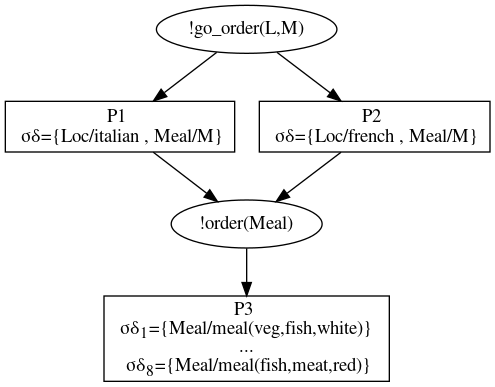
\includegraphics[width=0.70\linewidth]{ch_aamas2021/outfile.png}
  \caption{Goal-Plan Refinement of the Agent}
  \label{fig:gp-tree}
\end{figure}

In current implementations of BDI frameworks based on AgentSpeak(L), the three selection functions $S_E$, $S_O$, $S_I$ (respectively for events, plans/options, and intentions) are typically exposed as abstract functions that the designer can override to implement any type selection function. Although this approach promotes flexibility, the fact that part of the decision-making remains external to the agent script reduces readability, encapsulation, and transparency of the agent programs, and makes the control more opaque to the designer. For these reasons, the selection functions hardcoded should be kept as simple as possible.

Default implementations are based on selecting the first available option, which is indeed a good example of simplicity.
If we apply the default implementation also on this example, the first applicable unifier for \asc{!go_order(L,M)} is \asc{{Loc/italian, Meal/M}}, and the first applicable unifier for \asc{!order(S,M,W)} is \asc{{M/meal(veg,fish,white)}}.  %\Mos{Maybe you want to change this)}

%\Gio{[Here we should write that current execution of abstract plans do not look for all 8 configurations, they just take the first one which is retrieved satisfying the context conditions (typically depending on the order of beliefs specified in the program).}

\subsection{CP-Nets and CP-Theories}
\label{ssec:prefs}
%Recalling on the CP-Theories \cite{Wilson2004}, assume a set of variables $X \in V$ each having a set finite set of values $x$, deonted $Dom(X)$, called the \textit{domain} of $X$. A value $u$ for $U \subseteq V$ associates with every $X \in U$ a value of $X$. The set of all values $u$ for $U$ is denoted $Dom(U)$, called the domain of $U$ and $\top$ the only value of $U=\emptyset$. A conditional preference $\lambda$ on $V$ is denoted by $u:x \succ x'[W]$, where $U \subseteq V$, $u \in Dom(U)$, $X \in V - U$, $x,x' \in Dom(X)$, and $W \subseteq V - (U \cup \{X\})$. This preference relation means given $t \in Dom(T)$ where $T=V-(U\cup\{X\}\cup W)$, then $x$ is preferred to $x'$, irrespective of the value of $W$. CP-Nets \cite{Boutilier2004} can be presented with $W=\emptyset$.

%Based on this definitions, an outcome $o \in Dom(V)$
%\Mos{CP-nets and CP-Theories got very much intertwined here, need to clear up}

In order to specify preferences, we start from the definition of CP-Nets given in \cite{Boutilier2004}. Given a set of variables $X \in V$, each having a finite set of values $x$, conditional preference statements are in the form $u : x \succ x'$, where $x$, $x'$ are assignments of a variable $X \in V$, and $u$ is an assignment to a set of variables $U \subseteq V$ (parents of $X$). The interpretation of this statement is that given $u$, then $x$ is preferred to $x'$ all else equal, meaning, for all assignment $s$ of the set of variables $S$, where $S = V - (U \cup \{X\})$, $sux$ is preferred to $sux'$, where $sux$ and $sux'$ are two \textit{outcomes} (complete assignment) to all variables of $V$. 
CP-Theories are introduced in \cite{Wilson2004} to extend CP-Nets with \textit{stronger conditional statements}. These include preferential statements in the form $u : x \succ x' [W]$, where $W \subseteq V$ which interprets that for all assignments $w,w'$ to variables of $W$ and assignments $t$ to variables of $T = V - (U \cup {X} \cup W)$, then the outcome $tuxw$ is preferred to the outcome $tux'w'$. This means that given $u$ and any $t$, then $x$ is preferred to $x'$ \textit{regardless} of assignments to $W$.



%It is shown that with both CP-Nets and CP-Theories, a set of such preference statements $\Lambda$ generates a partial ordering between all the outcomes of $V$, if $\Lambda$ is consistent, where consistency corresponds to the preference relations being acyclic with respect to the parent child relations of the variables. 
Assuming $\Lambda$ is a set of acyclic (with respect to parent-child relations) preference relations over variables of $V$, and considering $o,o'$ are outcomes of $V$, then we say $\Lambda \models o \succ o'$ iff $o \succ o'$ satisfies every preference statement in $\Lambda$. 
%$\Lambda$ is satisfiable iff there exists a preference ranking $\succ$ over the outcomes of $V$ that each $o \succ o'$ satisfies each of the preference statements of $\Lambda$. It is said that $\Lambda \models o \succ o'$ iff $o \succ o'$ holds in every preference ordering that satisfies $\Lambda$. 
Then $o$ and $o'$ can have one of the possible relations according to $\Lambda$: either $\Lambda \models o \succ o'$; or $\Lambda \models o' \succ o$; or $\Lambda \not\models o \succ o'$ and $\Lambda \not\models o \succ o'$. The third case means there is not enough information to prove either outcome is preferred. 

Based on these definitions, two distinct ways for comparing outcomes are proposed in \cite{Boutilier2004}:
\begin{itemize}
    \item Dominance queries: Asking if $\Lambda \models o \succ o'$ holds, which is referred to as $o$ is preferred to and \textit{dominates} $o'$.
    \item Ordering queries: Asking if $\Lambda \not\models o' \succ o$ holds, which is referred to as $o$ is preferred to $o'$.
\end{itemize}
Although ordering queries are weaker than dominance queries, they are still sufficient in many applications, and will be used in this work. In particular, if an outcome $o$ is present such for all other outcomes $o'$ we have $\Lambda \not\models o' \succ o$, then we say $o$ is \textit{undominated} or \textit{most preferred} with respect to $\Lambda$.
%One of the main usages of such partial ordering is comparing outcomes, The are two distinct ways proposed by \cite{Boutilier2004}

All through this work, and for the sake of simplicity, only strict preferences $\succ$ are considered. Nevertheless, these semantics are shown to be extendable to weak preferences $\succeq$ and indifference $\sim$ in both CP-Nets and CP-Theories.

%While the idea of integrating CP-Nets (and CP-Theories) with BDI programs have been suggested before \cite{Mohajeri2019,Mohajeri2020}, there are important distinctions between the logic and algorithms defined for CP-Nets and those of BDI agents or even more broadly logic programs that need to be addressed. Firstly, by definition, CP-Nets rely on a closed world assumption, which means they assume a single static set of variables $V$ (or \textit{features} or \textit{attributes}) as the decision domain and all of the variables appearing in a conditional preference statement (or rule) should be part of $V$. Secondly, they focus attention on single-stage decision problems with complete information, ignoring any issues that arise in multi-stage, sequential decision analysis and any considerations of risk that arise in the context of uncertainty \cite{Boutilier2004}.% which means preference rules create a hierarchy between these variables.


%Contrary to CP-Nets, a BDI agent deals with many related or independent sets of variables in their decisions and can not be limited to one set. Also, a dynamic agent's factual, inferential, procedural or even preferential knowledge about the environment can be subject to revisions in the its life-cycle and it can not be assumed that all the variables are fully known at any point. Furthermore, BDI agents are designed to act in dynamic environments with incomplete information and uncertainty, and more often than not, a BDI agent deals with these issues via multi-stage decision making and dynamic reactions to the environment such as incremental plan and goal refinement and even failure handling.
\subsubsection{Embedding in BDI agents}
\label{sssec:transform}
To transform CP-Theories to a formalism that can be used with the Prolog-like inferential systems as those used in AgentSpeak(L) agents, one should look at what needs to be decided in the process of goal refinement. An agent may have dynamically interconnected beliefs about the environment, but when it is deciding on what is the most preferred approach to partially ground the variables of an event or goal in the form of e.g $!g(v_1,...,v_n)$, only the parameters of that goal are relevant to %part of 
the decision. Theoretically, in this approach we do not have only one CP-Theory, but each distinct goal/event has zero or more inferred CP-Theories from the set of all preference statements. 

In this work, the preferences of an agent are presented in a different notation from that of CP-Nets and CP-Theories, but more similar to OCP-Theories in \cite{DiNoia2015}.

A conditional preference statement $\lambda$ of the agent can be expressed in the form of inferential rules such as:
\begin{equation*}
    G \succ G' \leftarrow C
\end{equation*}
where $G,G'$ are either belief predicates in the form $g(v_1,...,v_n)$ and $g({v}_1',...,{v}'_n)$, or triggering events in the form $!g(v_1,...,v_n)$ and $!g({v}'_1,...,{v}'_n)$ (or any other type of trigger, $?,+,-$). Each $v_i$ and ${v}_i'$ can be either a (partially) ground term, a named variable or an anonymous variable (underscore, ``\texttt{\_}''), and $C$ is an arbitrary logical expression that \textit{activates} the preference statement if it can be proven to be true at the time of evaluation, which can include variables that appear on the left side of the $\leftarrow$. The set of all preferences of an agent is referred to as $\Lambda$.

With this definition, for each predicate $G$ with the form $g(v_1,...,v_n)$, we can denote its set of variables (or features or attributes) as $V_G = \{v_1,...v_n\}$. %The simplest form of preference statements that can be expressed with this form is that of CP-Theories. 
To express a preference statement $u : x \succ x' [W]$ in this form, on a predicate $G$, assuming $G_X \in V_G$ is the variable of $G$ corresponding to $X$, the set $G_U \subseteq V_G$ is the set of all variables corresponding to $U$, the set $G_W \subseteq V_G$ is the set of all variables corresponding to $W$ and $G_T = V_G - (G_U \cup \{G_X\} \cup G_W)$, the statement can be presented as $G \succ G' \leftarrow true$, such that $G_X$ is written as $x$, $G'_X$ is written as $x'$, all the variables of $G_U$ and $G'_U$ are written as their corresponding value in $u$, all variables of $G_W$ and $G'_W$ are written as anonymous variables (underscore) and all the variables of $G_T$ and $G'_T$ are replaced with named variables that have the same name in both $G$ and $G'$.

%For instance, a statement like $p(x,u,T,\_) \succ p(x',u,T,\_) \leftarrow true$ describes the preference holding between two (partially) grounded terms with the functor $p$. Any term whose first parameter can be grounded to $x$ is preferred to the one that its first variable can be ground to $x'$, if the second parameter can be unified to $u$ in both, the third parameter is the same,  regardless of the values of the fourth variables. 

Showing that these two forms of statements are equal is intuitive. For instance, given the statement of $g(x,u,T,\_) \succ g(x',u,T,\_) \leftarrow true$ and two (partially) grounded terms $g(t_1,...,t_4)$ and $g({t}'_1,...,{t}'_4)$, we can infer  $g(t_1,...,t_4) \succ g({t}'_1,...,{t}'_4)$ iff we have $t_1=x$, ${t}'_1=x'$ and $t_2={t}'_2=u$ and $t_3={t}'_3$ regardless of the values of $t_4$ and ${t}'_4$. By using induction we can see that the same can be inferred for any number or parameters that correspond to $G_U,G_W,G_T$ or with any other rearrangement of the parameters.


Pure CP-Theory (and by extension CP-Net) statements can be expressed in the form of $G \succ G' \leftarrow C$ where $C=true$, but, as BDI agents are designed to act in dynamic environments with incomplete information and uncertainty, and more often than not, a BDI agent has to react to changes in the environment and failures; simply using static CP-Theory statements is not sufficient for a BDI agent. This is addressed by the \textit{activation} condition $C$ of preference statements. This condition can be any arbitrary Prolog-like expression over the belief base of the agent. A preference statement is \textit{active} if the context condition can be proven from the belief base of the agent. Intuitively this means that the left side of the rule holds true if the right side can be proven. This can drastically increase the expressivity of the preference statements in dynamic environments.
%and the variables appearing on the left side of the $\leftarrow$. 
\begin{ddefinition}[Active Preference Statement]
At any point in the life-cycle of agent with a belief base $B$ and set of preference statements $\Lambda$, a preference statement $G \succ G' \leftarrow C$ is \textit{active} iff $C$ is a logical consequence of $B$. 
\end{ddefinition}



The next example further explores these type of preferences, and is an extended version of what is presented in the original CP-net paper \cite{Boutilier2004} to facilitate comparison.



%To extend the definition of $\succ$ to unifiers of a partially unbound term: given a database of facts and rule $B$ and a set of preferences $\Lambda$, if $\epsilon$ is a partially unbound term and $\delta,\delta'$ are two unifiers for $\epsilon$ such that $\epsilon\delta$ and $\epsilon\delta'$ are logical consequences of $B$, then if $\epsilon\delta \succ \epsilon\delta$


%Secondly, CP-Nets focus attention on single-stage decision problems with complete information, ignoring any issues that arise in multi-stage, sequential decision analysis and any considerations of risk that arise in the context of uncertainty \cite{Boutilier2004}. These limitations are mainly because CP-Nets require every possible value of each variable to be known prior to decision-making and also, a CP-Net needs to decide a value for each variable in the process of decision-making. These issues, are a detrimental contrast from BDI agents that are designed to act in dynamic environments with incomplete information and uncertainty, and more often than not, a BDI agent deals with these issues via multi-stage decision making and dynamic reactions to the environment such as incremental plan and goal refinement and even failure handling.
%  Furthermore, as the main point of this chapter, a BDI agent with partially grounded goals, does not need to decide on every variable of a variable set in their decision and some variables may stay unbounded.
%  unlike many other works on integrating preferences into BDI agents \cite{Visser2011,Visser2016,Mohajeri2019,Mohajeri2019Prefs}, this work does not assume that all the possible values for variables are known at any point in agent's life-cycle

%The third core difference between CP-Nets and BDI agents, or more precisely agents that utilize Prolog-like reasoning concerns the algorithms used for finding decisions. The variables of a 

%Prior to addressing these issues, first a formal definition of a conditional preference relation of an agent is presented, which informally describes a rule that in the condition $C$ the term $T$ dominates the term $T'$. 




%\begin{ddefinition}
%A conditional preference relationdenoted as $T \succ T' \leftarrow C$  given a database of facts and rules $B$, at any point in time, iff $C$ is a logical consequence of $B$.
%\end{ddefinition}

\subsubsection*{Example 3}
Let us consider some preferences over the actions of our food ordering agent, starting from some preferences over the meal: (R1) for the main course, meat is preferred to fish if at an Italian restaurant; (R2) fish is preferred to meat if at a French restaurant; (R3) if the main course is meat, then a fish soup is preferred to vegetable soup; (R4) if the main course is fish, then a vegetable soup is preferred; (R5) for drinks, red wine is preferred to \textit{any} other type of drink if vegetable soup is in the meal; likewise, (R6) white wine is preferred to \textit{any} other drinks if fish soup is in the meal. 

%Note that R1 and R2, are conditional based on external factors

%In these preferences only the first one is unconditional and the other four are conditional, also note that for example in the second preference relation, while an explicit condition is put on the meat course or variable \asc{M}, there is also an implicit condition on the wine or \asc{W}, which dictates that in order for this preference relation to be applicable between two meals, the wine should be the same, this represents the \textit{all-else-equal} principle of the CP-Nets. 

While multiple preferences are defined over the meal, still they do not translate directly to any of the events that the agent can handle. To fix this, we add a simple but important (meta-)preference: (R7) in the event of ordering \textit{anything}, ordering something more preferred is also preferred to ordering something less preferred.% While this preference connection may seem obvious, defining such arbitrary preference relations can prove to be a powerful tool for the designer in many cases.
We define at this point a few preferences about the restaurant: (R8) if the agent is already located at a restaurant, it is preferred to order at that restaurant (i.e. not to move) compared to {any} other restaurant, regardless of the meal; (R9) the combination of Italian restaurant with a meat main dish is preferred to any other restaurant and main dish combination if the agent is not already at another restaurant. The specification of these preferences can be seen in listing \ref{lst:prefs_1}. A more detailed and practical explanation of how these statements are written as Prolog rules can be found in section \ref{sec:implementation}.

%Note that preference relation R1, R2, R8 and R9 are different from the rest because they are conditional based on the belief base of the agent and will be active if their condition is a logical consequence of the belief base $B$ at the time of plan selection. 

\begin{listing}[t]
\centering
\begin{tcolorbox}[left=2pt,right=2pt,top=2pt,bottom=2pt,arc=0pt,
                  boxrule=0pt,toprule=1pt,
                  colback=white]
\begin{minted}[fontsize=\footnotesize,linenos]{prolog}
(R1) meal(S,meat,W) >> meal(S,fish,W) :- at(italian).
(R2) meal(S,fish,W) >> meal(S,meat,W) :- at(french).
(R3) meal(fish,meat,W) >> meal(veg,meat,W) :- true.
(R4) meal(veg,fish,W) >> meal(fish,fish,W) :- true.
(R5) meal(veg,M,red) >> meal(veg,M,_) :- true.
(R6) meal(fish,M,white) >> meal(fish,M,_) :- true.
(R7) !order(M1) >> !order(M2) :- M1 >> M2.
(R8) !go_order(L,_) >> !go_order(_,_) :- at(L).
(R9) !go_order(italian, meal(S,meat,W)) 
     >> !go_eat(L,meal(S,_,W)) :-  not at(L).
\end{minted}
\end{tcolorbox}
    \caption{Preferences of Food-ordering agent}
    \label{lst:prefs_1}

\end{listing}

We can draw as in Figure~\ref{fig:cp-graph} the preferential relation graph associated to the predicate \asc{meal/3} with respect to preferences in listing \ref{lst:prefs_1} and the beliefs in listing \ref{lst:beliefs_1}. The graph clearly suggests that, in this context, \asc{meal(veg,fish,red)} is the most preferred (undominated) option. Note however that this graph would have been different if the agent had the belief \asc{at(italian)} instead of \asc{at(french)}. %which intuitively means the agent has different preferences about meals in different restaurants. 

\subsubsection{Generalization}

The preference statements in listing \ref{lst:prefs_1} have been chosen because they offer a good representation of the possible uses of the proposed method, and can be easily generalized. First of all, we observe that only R3 and R4 are pure CP-Theory preferences. The statements R1, R2 are conditioned on beliefs that are external with respect to the variables of the preference itself (in this case, the location of the agent). This type of conditional statements result in multiple preferential relations that may also be contradictory. % In fact, the preference structure in figure~\ref{fig:cp-graph} would have been different if the agent had the belief \asc{at(italian)} instead of \asc{at(french)} which intuitively means the agent has different preferences about meals in different restaurants. 
%Although, this only works because it is assumed that at most one of the two conditions \asc{at(french),at(italian)} can be true at any time and in fact, 
For instance, if both conditions \asc{at(french)} and \asc{at(italian)} were true at any time, then the two preferences would be contradictory and the preference relations concerning \asc{meal/3} would be unsatisfiable.
%Furthermore, as other statements over \asc{meal/3} are dependant on (are child nodes of) the main dish, there are two different preferential structures associated to this predicate as shown in figure~\ref{fig:cp-graph}. 

The statements R5 and R6 specify preferences that, although simple, can not be expressed in standard CP-Theories, as they give conditional preference to a value of a variable (drinks) over any other value of that variable (\textit{erga omnes} preference); this can be very useful in cases where the domain of values of a variable are unknown at design time, but the designer is aware of a few values that are always either desired or to be avoided. 

As it was already observed, R7 is a meta-preference. The condition of this statement does not consult the belief-base of the agent, but rather the preferences of the agent. It works as a mapping of a preference expressed as object level to a preference expressed as action level. In general, any preference over objects is implicitly referring to a certain domain of activities, and it is as such only a more compact representation. Preferences as R7 are needed to make explicit this connection. The technical aspects of this step will be explained more in detail in section \ref{sec:implementation}. 

The statement R8 is conditional over a belief that the agent may have (\asc{at(L)}), and also connects the variable of this condition \asc{L} (that will be grounded at run-time) to the preference relation itself, creating an interesting \textit{parameterized} preference structure capturing in this case ``\textit{I prefer the place I am already at}''. 

Finally, also R9  presents a statement that can not be expressed in CP-Theories, in which two different variables are part of the preference. This can be useful tool but also can easily lead to cyclic preferences, thus, this type of preference statement should be used with care. 

%\Gio{[I find all this very interesting. But I have a natural question: can we apply still the method of CP-theory for constructs which are not CP-theories? Is it valid/sound?]}

\begin{figure}[!tbh]
  \centering
  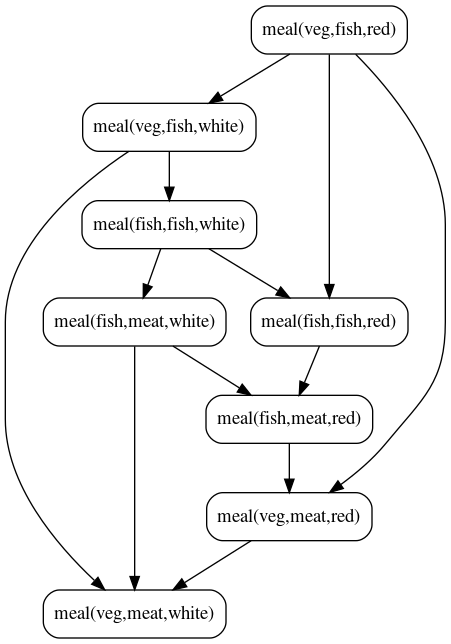
\includegraphics[width=0.5\linewidth]{ch_aamas2021/cp-graph.png}
  \caption{Preference Structure of the Agent over \asc{meal/3}}
  \label{fig:cp-graph}
  
\end{figure}

\subsection{Goal Refinement via Preferences}
\label{ssec:goalref}
The integration of preferences into the BDI reasoning cycle can be implemented as a \textit{unifier ordering} step prior the \textit{plan selection}, that only applies when the triggering event contains unbounded variables. To achieve this, when the agent selects a partially unbounded event $\epsilon$, first it needs to find all the relevant unifiers by consulting the plan library, and then find all the applicable unifiers by consulting the belief base. Afterwards, the agent can create a partial ordering between the applicable unifiers. 

To extend the definition of section \ref{ssec:prefs} to unifiers, assuming $\epsilon$ is a partially unbound event and $(\sigma\delta),(\sigma\delta)'$ are two applicable unifiers for $\epsilon$, we say $(\sigma\delta) \succ (\sigma\delta)'$ satisfies a preference statement $G \succ G' \leftarrow C$ if $\epsilon(\sigma\delta)$ can be unified with $G$ and $\epsilon(\sigma\delta)'$ can be unified with $G'$. Given  $\Lambda$, a set of acyclic preference statements in this form, then we say $\Lambda \models (\sigma\delta) \succ (\sigma\delta)'$ iff $(\sigma\delta) \succ (\sigma\delta)'$ satisfies every active preference statement in $\Lambda$. We can then say $(\sigma\delta)$ is \textit{preferred} to $(\sigma\delta)'$ iff $\Lambda \not\models (\sigma\delta)' \succ (\sigma\delta)$. An then we can define the \textit{undominated} or \textit{most preferred} unifier:

\begin{ddefinition}[Most preferred unifier]
\label{def:mpu}
A unifier $(\sigma\delta)$ is referred to as an \textit{undominated} or \textit{most preferred} unifier for an event $\epsilon$ iff $\sigma\delta$ is an applicable unifier for $\epsilon$ and for every other applicable unifier $(\sigma\delta)'$ we have $\Lambda \not\models (\sigma\delta)' \succ (\sigma\delta)$.
\end{ddefinition}

Surprisingly, with this definition, finding the most preferred unifier is simple in a Prolog program as it matches well with how Prolog engines work. Normally in a Prolog program it is not easy to query if a fact holds with respect to every rule concerning that fact, but if a query about a fact fails, this means that all the rules about that fact have failed i.e, that the fact can not be proven. Thus, to find if a unifer $(\sigma\delta)$ is the most preferred one for an event $\epsilon$, it is enough to ask if for every other unifier $(\sigma\delta)'$, the query $(\sigma\delta)' \succ (\sigma\delta)$ fails. Intuitively, running this query for every unifier of $\epsilon$ will result in finding the most preferred unifier. More details on the implementation of this algorithm is presented in section \ref{sec:implementation}.

%Assuming $\Lambda$ is a set of acyclic (with respect to parent-child relations) preference relations over variables of $V$, and considering $o,o'$ are outcomes of $V$, then we say $\Lambda \models o \succ o'$ iff $o \succ o'$ satisfies every preference statement in $\Lambda$. 
%$\Lambda$ is satisfiable iff there exists a preference ranking $\succ$ over the outcomes of $V$ that each $o \succ o'$ satisfies each of the preference statements of $\Lambda$. It is said that $\Lambda \models o \succ o'$ iff $o \succ o'$ holds in every preference ordering that satisfies $\Lambda$. 
%Then $o$ and $o'$ can have one of the possible relations according to $\Lambda$: either $\Lambda \models o \succ o'$; or $\Lambda \models o' \succ o$; or $\Lambda \not\models o \succ o'$ and $\Lambda \not\models o \succ o'$. The third case means there is not enough information to prove either outcome is preferred.

%, then $\Lambda$ is satisfiable iff there exists a preference ranking $\succ$ over the applicable unifiers of $\epsilon$ that each $(\sigma\delta) \succ (\sigma\delta)'$ satisfies each of the preference statements of $\Lambda$. 
%it is said that $\Lambda \models (\sigma\delta) \succ (\sigma\delta)'$ iff $(\sigma\delta) \succ (\sigma\delta)'$ holds in every preference ordering that satisfies $\Lambda$.




%In this ordering, a an applicable unifier $(\sigma\delta)$ precedes another applicable unifier $(\sigma\delta')$ for $\epsilon$, if $\epsilon(\sigma\delta)$ is not dominated by $\epsilon(\sigma\delta)'$ according to the preferences. Note that this will result in a partial ordering and some unifiers may be incomparable depending on the preferences. 


%With this approach, %the normal plan selection can continue w.r.t. the re-ordered list of unifiers, but now, 
%the plan selection function can take into account the ordering between unifiers. Through the rest of the chapter, f
For simplicity, it is assumed that the agent uses the plan selection function typical in BDI frameworks, i.e. selecting the first applicable unifier for each event. This assumption means that the agent always uses an \textit{undominated} or \textit{most preferred} unifier to ground the variables of a (partially) abstract goal if this unifier exists, or reverts to the default behavior of selecting the first applicable unifier in case of inconsistencies with preferences that may result in situations that no unifier is the most preferred.
%Note that the event does not need to be fully grounded and it may be that the unifier $\sigma$ keeps some of the variables unbounded or even introduce new variables. As this unifier 



\subsubsection*{Example 4}
Consider again the agent script given in example 1, with the beliefs of example 2, and with the preferences of example 3. Assume that this agent receives an abstract event \asc{!go_order(L,M)}. Then, as in example 2, two applicable unifiers will be created. P1 will be applicable with the unifier \asc{{Loc/italian, Meal/M}} and P2 with the unifier \asc{{Loc/french, Meal/M}}. Because the agent has the belief \asc{at(french)}, we can see that the relation:
\begin{minted}[fontsize=\small]{prolog}
!go_order(italian,M) >> !go_order(french,M)
\end{minted}
can not be proven from the preferences (R8 and R9 can not conclude it) but the relation:
\begin{minted}[fontsize=\small]{prolog}
!go_order(french,M) >> !go_order(italian,M)
\end{minted}
can be proven to be true (based on R8), so
% \begin{minted}[fontsize=\small]{prolog}
% !go_order(french,M) >> !go_order(italian,M)
% \end{minted}
the \asc{{Loc/french, Meal/M}} is the single most preferred unifier and P2 will be selected as this is the only plan applicable with this unifier. Next, when the sub-goal \asc{!order(Meal)} is being considered, there are 8 applicable unifiers for plan P3, assuming the \asc{at(french)} belief still stands, and based on the given preference rules, the ordering in Fig.~\ref{fig:cp-graph} will apply, and then the most preferred unifier will be \asc{{S/veg, M/fish, W/red}}. This means that the abstract goal will be refined to \asc{!order(meal(veg,fish,red))} and consequently plan selection will instantiate the plan associated to it (P3).

\subsubsection*{Example 5}
To show how partially abstract goals would be grounded with this method, consider the same agent as before with the same set of preferences and beliefs, except this time the agent has the belief \asc{at(home)} instead of \asc{at(french)}, and the agent receives an event with ordering a meal with meat as the main course:
\begin{minted}[fontsize=\small]{prolog}
!go_order(L,meal(S,meat,W)). 
\end{minted}
This time plan P2 will be applicable with two unifiers:
\begin{minted}[fontsize=\small]{prolog}
{Loc/italian, Meal/meal(S,meat,W)}
{Loc/french, Meal/meal(S,meat,W)}
\end{minted}
because the agent has the belief \asc{at(home)}, the statement R8 is not active for any of the unifiers and based on the the statement R9, the Italian restaurant is preferred to any other restaurant as long as there is meat main course, so again while the relation:
\begin{minted}[fontsize=\footnotesize]{prolog}
!go_order(italian,meal(S,meat,W)) >> !go_order(french,meal(S,meat,W))
\end{minted}
can be proven (based on R9), but the relation:
\begin{minted}[fontsize=\footnotesize]{prolog}
!go_order(french,meal(S,meat,W)) >> !go_order(italian,meal(S,meat,W))
\end{minted}
can not be proven from the preference statements (R8 and R9 can not conclude it), so the first unifier will be the most preferred one and then P2 is selected with it. Next, assuming the \asc{move_to} action works correctly, the belief \asc{at(home)} will be retracted, \asc{at(italian)} will be added to the belief-base, and the sub-goal \asc{!order(meal(S,meat,W))} will be adopted. At this point (see the example in \cite{Boutilier2004}), based on the preference statements and agent's beliefs, the most preferred unifier will be \asc{{S/fish, M/meat, W/white}}, meaning the goal will be refined to \asc{!order(meal(fish,meat,white))}, and then the plan for this goal (P3) will be instantiated by the plan selection.

An interesting point in this example is the interaction between preference statements R1 and R9. In normal CP-Nets, these two statements makes the network cyclic: the preference over main dish is dependent on the location (R1), and the preference over the location depends on the main dish (R9). But in this work such preferences can be defined for two reasons: (1) \textit{framing}, meaning the two preferences, although being about the same variables, are defined in two different frames of choice, and (2) \textit{context}, meaning that as the agent resides and acts in a dynamic environment, it perceives changes and modifies its beliefs, which in turn modifies the agent's preferences, e.g. while the agent has the belief \asc{at(home)}, R1 and R2 are not active and so they are not part of unifier selection process. 

%\Mos{NEED TO WRITE ABOUT THE TEMPORAL ASPECT OF THIS EXAMPLE HERE OR LATER ON, IN NORMAL CP-NETS THIS IS A CYCLE, FOOD DEPENDED ON LOCATION AND LOCATION DEPENDED ON FOOD, BUT HERE BECAUSE THERE ARE DIFFERENT CHOICE POINTS ITS NOT A PROBLEM}

%\Gio{[Very interesting. I would write it here]} 

\section{Implementation\label{sec:implementation}}

This section presents a practical implementation
of the transformation method from CP-Theory logic to Prolog logic proposed in section \ref{sssec:transform}. 

\subsubsection*{Preference operator}
First, we need to express a preference statement $G1 \succ G2 \leftarrow C$, where $G1,G2$ are partially grounded terms with the same functor and arity. The mapping from CP-Theory statements to this statement is presented in section \ref{sssec:transform}. This binary operator $\succ$ will be introduced both into the syntax of the agent programming language and as a binary predicate into the belief base of the agent. In the syntax, the operator $\succ$ will be denoted as \asc{>>} making a relation such as $G1 \succ G2$ to be written as \asc{G1 >> G2}.
%Interestingly, as this operator is simply there to define a relation between two terms, it does not need any extra logic attached to it. In fact, this method can be implemented even without introducing a new operator to the syntax by instead using a predefined binary predicate such as \asc{preferred/2}, this way a preference relation $G1 \succ G2$ can be written as \asc{preferred(G1,G2)} instead. 
To write full contextually conditioned statements as $G1 \succ G2 \leftarrow C$, we can utilize the Prolog inference rules. The former preference statement can then be written as \asc{G1 >> G2 :- C}. %With this way of writing, at any point in run-time, given two partially ground terms \asc{g1,g2} then \asc{g1 >> g2} is considered a logical consequence of the belief base if there is a correct 

\subsubsection*{Applicability} Next, as the method is implemented by utilizing the belief-base of the agent, a modification is needed to allow preference statements about different types of \textit{goals} to be part of the belief base, as e.g. in the R8 statement from listing \ref{lst:prefs_1}. To do this, a supplementary predicate $applicable/2$ is introduced. When a preference statement $G1 \succ G2 \leftarrow C$ is defined where $G1$ and $G2$ are triggering events e.g. achievement goal ($!G$), test goal ($?G$), the preference statement is transformed at compile/interpretation time to:
\begin{equation*}
applicable(t,G1) \succ applicable(t,G2) \leftarrow C
\end{equation*}
where $t$ is a predefined atom describing the type of the event, e.g: the preference statement R8 in listing \ref{lst:prefs_1} will be rewritten as:
\begin{minted}[fontsize=\small]{prolog}
applicable(achievement,go_order(L,_)) 
    >> applicable(achievement,go_order(_,_)) 
    :- at(L).
\end{minted}
As this is a normal Prolog rule, it can be simply added to the belief base of the agent. Then, preference relations can be queried from any context, as e.g. the (meta-)preference R7 in listing \ref{lst:prefs_1}, in which a preference relation is used as the condition of another preference, or, more importantly, to exploit Prolog queries to find the most preferred unifier for abstract events.

\subsubsection*{Optimality}
Next, the algorithm should be implemented for finding an optimal outcome, that is, the most preferred unifier(s) for a partially abstract term. The algorithms originally introduced for CP-Nets and CP-Theories generate an optimal outcome by \textit{sweeping} through the network from top to bottom (i.e., from ancestors to descendants) setting each variable to its most preferred value given the instantiation of its parents. While these algorithms are efficient and intuitive, they are not applicable for the transformed Prolog-like rules. Unlike CP-Nets and CP-Theories, the preferential structure of an agent is not static because of the presence of extra-contextual conditions; also, with the new form of statements, the parent-child relation of the variables is not explicit anymore. For these reasons, new algorithms are needed that do not rely on the hierarchy of the variables but instead utilize the backtracking feature of Prolog. 

Looking at the definition \ref{def:mpu}, given a set of preference statements as Prolog rules in a belief base $B$, to prove that a unifier $(\sigma\delta)$ is the most preferred unifier for a partially unbound term (or event) $\epsilon$, it is sufficient to prove that for every other unifier $(\sigma\delta)'$ of that term, the relation $\epsilon(\sigma\delta)' \succ \epsilon(\sigma\delta)$ is not a logical consequence of $B$. Intuitively with the semantics of Prolog, this means that this relation could not be concluded from any of the preference statements of $B$. With this, a simple algorithm that can find the most preferred (or undominated) unifier(s) for a partially unbound term is a backtracking search that goes through every possible (partial) grounding of that term to find one where there is no other (partial) grounding of that term which is more preferred to it. Such algorithm can be implemented by adding the Prolog rule presented in Listing~\ref{lst:pref_alg} to the agent's belief base. The \asc{copy_term/2} is a standard predicate in many Prolog implementations that unifies \asc{G2} with a copy of \asc{G} in which all variables are replaced by new variables. 
\begin{listing}[!ht]
\centering
\begin{tcolorbox}[left=2pt,right=2pt,top=2pt,bottom=2pt,arc=0pt,
                  boxrule=0pt,toprule=1pt,
                  colback=white]
\begin{minted}[fontsize=\small,linenos]{prolog}
most_preferred(G) :- 
    copy_term(G, G2), G, 
    forall((G2, (G2 >> G) -> fail; true)).
\end{minted}
\end{tcolorbox}
\caption{CP-Net reasoning algorithm implemented in Prolog}
\label{lst:pref_alg}

\end{listing}

% have been replaced by brand new variables, and all mutables by brand new mutables''. 
When this rule is queried with a partially unbound term \asc{G}, first a copy of \asc{G} is created as \asc{G2}, then the term \asc{G} itself is called, starting a backtracking search over all possible groundings of \asc{G}, and then \asc{forall/2} predicate starts a nested loop over all groundings of \asc{G2} and fails if it can find a grounding of \asc{G2} that \asc{(G2 >> G)}, otherwise if no such \asc{G2} is found it returns true meaning the current grounding of \asc{G} is the most preferred one. Also with how prolog queries work, if there is more than one most preferred (undominated) grounding, asking for more answers will return them.

There is one final rule needed to make this algorithm work which should be added to the belief base of the agent: \asc{T >> T :- !,fail.} which defines that a term can not be preferred to itself. With these rules added to the belief base, given a partially unbound term, we can run queries to find the most preferred unifier for that term. If we consider the example agent, querying the belief base with the term \asc{most_preferred(meal(S,M,W))} will give the result in one answer with the unifier \asc{{S/veg, M/fish, W/red}}. 

\subsubsection*{Embedding in the decision-making cycle}
Now that the belief base can answer queries about the most preferred unifier for a term, the next step is to allow the agent's reasoning engine to ask queries about the most preferred unifier for an event. To do this, the $applicable/2$ predicate that was defined before is used again. At compile/interpretation time, for each plan of the form $e : C \Rightarrow H$ a Prolog rule is added to the belief base of the agent in the form of:
\begin{equation*}
applicable(t,G) \leftarrow C
\end{equation*}
where $t$ is an atom that represents the type of the event $e$ and $G$ is the term associated with $e$. As an example, the rule for plan P1 is:
\begin{minted}[fontsize=\small]{prolog}
applicable(achievement,go_eat(L,M)) :-
    restaurant(L) & not at(L)
\end{minted}
Intuitively, at any moment in run-time, by querying this predicate, we can retrieve all possible applicable groundings of an event that can be concluded from the plan library and the belief base. For instance, by querying the term  \asc{applicable(achievement,go_eat(L,M))}
on the belief base of an agent with the beliefs, plans and preferences described in section \ref{sec:method}, the agent obtains two answers: \asc{{L/italian, M/M}} and \asc{{L/french, M/M}}. Then, by using this predicate with combination of \asc{most_preferred/2}, the agent can find the \textit{most preferred applicable unifier} for an event. This is possible because the preference statements about events were already transformed with the \asc{applicable} predicate. Considering our running example, by querying the term 
\begin{minted}[fontsize=\small]{prolog}
most_preferred(applicable(achievement,go_eat(L,M)))
\end{minted}
only one answer \asc{{L/french, M/M}} will be returned. Now to embed the goal refinement step into the agent reasoning cycle.
%is trivial, yet depending on the framework at hand. In general, only minimal modifications are required: 
After the event selection step, if the selected event $\epsilon$ contains free variables, then the most preferred unifier(s) should be found for this event by querying the belief base of the agent with the aforementioned method, and the resulting answer(s) are sent to the plan selection function.


\subsubsection*{Complexity}
%Calculating the time complexity of the algorithm is rather simple, 
The core of the method is the rule for the predicate \asc{most_preferred/1}, and this rule has two nested backtracking loops over the possible groundings of the input term. In the worst case scenario, each two groundings of a term should be queried with all of the preference statements associated to that rule. Then, for a term $T$, if the there are $n$ number of possible groundings at any time, and there are $m$ preference statements over $T$, then, in the worst case scenario, the time complexity of finding the most preferred unifier will be $n^2 \times m$. 

%\Gio{[What about the complexity of CP-nets/CP-theories? I would also add something like. Such worst-case scenario can be reduced by optimizing the relative positions of preferential rules and groundings in the belief base, for instance by exploiting statistical information concerning their applicability or relevance for the decision-making cycle. Note that this information depends on the coupling agent-environment, and a structural change in the workings of one of the two would demand a recomputation of the relative positions of rules and facts.]}



\section{Discussion and conclusion}
\label{sec:discuss}
This chapter contributes to recent efforts to integrate preferences into BDI agents. Despite the `D' in the acronym, desires play a limited role in contemporary BDI agent platforms, as they are generally conflated to goals (procedural or declarative). This chapter showed that by interacting adequately with the belief base and plan library of the agent, abstract goals can be refined taking into considerations the agent's preferences. Stated differently, preferences act here as background desires modifying/impacting goals, playing the role in turn of contingent desires. (Note that in general the literature suggests that preferences are
derived from desires \cite{Lorini2017}; for our purposes, however, we discovered that the two can be seen as filling the same functional niche.) 

Although this work illustrated the use of preferences focusing on a single agent and on goal refinement, preference statements can be relevant in other contexts too. For instance, MAS frameworks allow agents to communicate and transmit their beliefs to each other. Leveraging the present proposal, because preference statements are implemented as beliefs, agents can directly communicate their preferences to other agents. This can be very useful e.g. in social simulation or social learning contexts, where the agents may need to decide to act (or not to act) depending on both their own and other agents' preferences. Another interesting use-case for this approach could be the implementation of normative agents, utilizing preference both to capture personal and societal norms (see the use of CP-nets for deontic logic in \cite{Sartor2020}).

Preference statements introduced in this work are in a form processable in Prolog logic programs. We have shown that a subset of this form can be used to express pure CP-Theory preferences. However, this new form can also be used to express contextually conditioned and parameterized preferences, resulting in much more flexibility than pure CP-Theories. Consider for instance the statement R8 in example 3: ``\textit{I prefer the place I am already at}''; that depends completely on the state of the agent in the environment and, if the environment is unknown and unpredictable, so will be the preference statement. 
Also, unlike CP-Theories that are fully qualitative, with the proposed form quantitative preferences can be expressed by using arbitrary arithmetic equations in the context condition of preferences; e.g: consider a statement ``\textit{I prefer a cheaper restaurant to a more expensive one}'' that can easily be expressed in this form with an arithmetic comparison as the condition of the statement.
But this flexibility %comes also
%Although this flexibility is needed to express the complex preferences of agents that acts in highly dynamic and unpredictable environments, it 
comes at the cost of static verifiability. Many of the preferences that can be expressed in the proposed representational model %could 
cannot be statically verified or predicted easily prior to run-time. The redeeming aspect of this problem is that static verification of dynamic agents is well-known to be a challenging task, especially in dynamic environments \cite{Fisher2020,Ferrando2019}. This explains the existence of run-time verification approaches for agent programming frameworks, and probably the most notable works that adopt a (semi-)formal run-time model checking approach to verification are those of the AJPF/MCAPL framework \cite{Dennis2012,Dennis2016}. These approaches are in principle also usable for agents that are enhanced with preferences.

Finally, one of the main requirement behind this work is accessible usability. The transformation method from CP-Theory preference statements to Prolog-like programs has been conceived to enable its use almost directly with AgentSpeak(L)-like frameworks \cite{Bordini2005,Astra,mohajeriparizi_2020_run,Aschermann2018}. Indeed, no extra reasoning component is introduced, all the preference reasoning and algorithms required for goal refinement is done through beliefs and inferential rules. Furthermore, unlike many of the works that embed preferences into BDI frameworks, e.g. \cite{Visser2011,Visser2016,Dasgupta2010,Mohajeri2019,Mohajeri2020}, this approach does not require any extra annotation of the agent's script with information about effects of plans or actions and thus makes it more accessible for the designer. 

A concrete Prolog implementation of ordering queries of CP-Nets/CP-Theories was presented, and a working proof of concept for this approach is publicly available\footnote{anonymized}. Analyzing its complexity, we showed that the proposed algorithm run in polynomial time. Such worst-case scenario could be however reduced by optimizing the relative positions of preferential rules and groundings in the belief base, for instance by exploiting statistical information concerning their applicability or relevance for the decision-making cycle. %Note that this information depends on the coupling agent-environment, and a structural change in the workings of one of the two would demand a recomputation of the relative positions of rules and facts.

% We believe that for these reasons, this method can be easily implemented in many of the existing BDI frameworks and a working proof of concept for this approach have been implemented\footnote{anonymized}.



\chapter{Interoperability and Automated Tests: DevOps}

Previous chapters introduced different tools and approaches for modelling norm-governed cyber-infrastructures, however, what typically holds such approaches back for real world applications is usability and adoptability for designers and models. Development solutions, such as testing and integration, undeniably play a central role in the daily practice of software engineering, and this explains why better and more efficient libraries and services are continuously made available to developers and designers. Could the MAS developers community similarly benefit from utilizing state-of-the-art testing approaches? The chapter investigates the possibility of bringing  modern software testing and integration tools as those used in mainstream software engineering into multi-agent systems engineering. Our contribution explores and illustrates, by means of a concrete example, the possible interactions between the agent-based programming framework ASC2 (AgentScript Cross-Compiler)  and various testing approaches (unit/agent testing, integration/system testing, continuous integration) and elaborate on how the design choices of ASC2 enable these interactions.


\section{Introduction}

Software testing is attracting increased interest in industry \cite{market_reports_2019} and it is one of the most used methods of software verification. One of the reasons of this success lies in the advancement and popularization in the software engineering community of methodologies commonly known as \textit{DevOps}, in particular of techniques of automated testing in \textit{continuous integration} (CI). Generally, CI refers to the facilitation provided by third-party tools for automating the build/test process of a software. In recent years, online DevOps services such as TravisCI\footnote{\url{https://travis-ci.com/}} and CircleCI\footnote{\url{https://circleci.com/}} have been increasingly used by software engineers to improve the efficiency of their testing process, a practice which plausibly resulted in increased quality of the developed software.

Very recently, Fisher et al. \cite{Fisher2020} have suggested that testing approaches would be an important complement to formal approaches to MAS verification, if they could be automated and integrated in a seamless way into MAS development. In our view, seamless integration  does not mean only that agent programmers are able to use the vast amount of software testing tools available to mainstream languages like Java or Python, but, more importantly, that they are also able to use (almost) language- and framework- agnostic online services as those used for CI. This chapter explores this idea, aiming to illustrate what the MAS community could gain by using industry standard testing tools and discussing what would be the theoretical and practical trade-offs for this choice. We investigate possible interactions of testing with agent-based programming, and its relation with other verification techniques. More concretely, we demonstrate various approaches to enhance the productivity of MAS development cycle in the ASC2 framework via mainstream software testing and integration tools, and elaborate on the design choices of ASC2 that affect the testability of agent-programs with the mentioned tools. Then, we explore on how this approach can be generalized for other MAS frameworks.

The motivation for this chapter arises from research conducted
% This work is motivated by the applied research
%domain focuses 
on data-sharing infrastructures (e.g. data marketplaces). At functional level, a data-sharing application corresponds to a coordination of several computational actors distributed over multi-domain networks. Those actors generally include certifiers, auditors, and other actors having monitoring and enforcement roles, ensuring some level of security and trustworthiness on data processing \cite{Zhou2020}.  Typically distributed across several jurisdictions, networks may be subjected to distinct norms and policies, to be added to  various infrastructural policies provided at domain level and \textit{ad-hoc} policies set up by the users. Some of these norms, as for instance the GDPR, bind  processing to conditions and specific purposes, but, more in general, all compliance checking on social systems requires to know and to infer (in case of a failure on expectations) \textit{why} an actor is performing certain operations. 
% As this example shows, regulating these infrastructures requires reproducing to a certain extent constructs similar to those observed in human reasoning (e.g. For which purpose is the agent asking access to the resource? On which basis is the infrastructure granting access?). For traceability and explainability reasons, decisions concerning actions need to be processed by the infrastructure as much as relevant operational aspects. 
Agent-based programming, and particularly the Belief-Desire-Intention (BDI) model, by looking at computational agents as \textit{intentional agents}, provides the ``purpose'' level of abstraction available by design, and for this reason it is a natural technological candidate for this application domain. 

The BDI model been extensively investigated as basis to represent computational agents that exhibit rational behaviour \cite{Herzig2017}.
%and multiple programming languages and frameworks have been introduced based on it, as AgentSpeak(L)/Jason \cite{RaoAS1996,Bordini2005}, 3APL/2APL \cite{Dastani2APL}, and GOAL \cite{Hindriks2009a}.
Recent works as e.g. \cite{Kampik2020} investigated various issues holding when mapping logic-oriented agent-based programs into an operational setting. In contrast, this chapter focuses instead on the \textit{development practice} aspect: as soon as we attempted to program data-sharing applications as agents, we experienced the lack of  mature software engineering toolboxes, thus hindering a continuous integration with the infrastructural-level components developed in parallel by our colleagues.

%Agent-based programming, and in particular the Belief-Desire-Intention (BDI) model by looking at computational agents as \textit{intentional agents}, provides this level of abstraction available by design, and for this reason, it is in principle a serious technological candidate for this application domain.  Recent works as e.g. \cite{Kampik2020,MohajeriParizi2020} investigated various issues holding when mapping logic-oriented agent-based programs into an operational setting. This chapter focuses instead on the \textit{development practice} aspect: as soon as we attempted to program data-sharing applications as agents, we experienced the lack of  mature software engineering toolboxes, thus hindering a continuous integration with the infrastructural-level components developed in parallel by our colleagues.

The document proceeds as follows: section \ref{sec:back} provides a background and related works on verification of MAS, in section \ref{sec:approach} we introduce our approach on MAS testing in ASC2 framework with mainstream tools. An illustrative example of this approach is presented in section \ref{sec:example}. Finally, section \ref{sec:discussion} provides the discussion and comments on possible extensions and future developments.

% a possible approach allowing seamless integration of modern software testing tools and services with agent-based and multi-agent systems programming.
% Furthermore this work presents an approach for seamless integration of modern software testing tools and services into both agent-based programming and multi-agent systems.



%Software testing is a series of processes, designed to make sure a computational entity does what it was designed to do and it does not do anything unintended. Testing allows the development teams to have some degree of assurance about the behaviors of different pieces of their product \cite{ArtOfTesting}.

% Furthermore, now that intelligent and autonomous systems are becoming more integrated in everyday life of humans, practical approaches for verification of such systems also become more crucial \cite{Fisher2020}. 
%Software testing is typically integrated as part of the development cycle which means it can be done in a iterative and agile manner and for many applications it can efficiently provide a sufficient level of assurance for the development team \cite{Fisher2020}.

\section{Verification of 
(Multi-)Agent Systems}
\label{sec:back}
% \begin{comment} % I would put that in another point
% \subsection{Belief-Desire-Intention (BDI) Model}

% At the agent level, in this chapter we  specifically explore testing of agents specified in the the \textit{belief-desire-intention} (BDI) model of agency. Having its roots in a theory of mind \cite{bratman1987intention}, and so referring to categories that are used typically to address human behaviour to describe agents, the BDI model \cite{Rao1995} has been extensively investigated as basis to represent computational agents that exhibit rational behaviour \cite{Herzig2017}. 
% % uses taxonomies that are used typically to address human behaviour to describe agents.
% \textit{Beliefs} are the factual (and possibly inferential) information the agent has about itself and its environment. \textit{Desires}, in their simplest form, are objectives the agent wants to accomplish. % \Gio{(i.e. facts desired to be true)}.
% %in the environment. 
% \textit{Intentions} are the courses of action the agent has committed to. In practice, BDI agents include concepts of \textit{Goals} and \textit{Plans}. Goals are instantiated desires % associated to reactive behaviors to certain events 
% and plans are abstract specifications relating a goal to the means of achieving that goal (intentions become commitment towards plans). Multiple programming languages and frameworks have been introduced based on the BDI model, as AgentSpeak(L)/Jason \cite{RaoAS1996,Bordini2005}, 3APL/2APL \cite{Dastani2APL}, GOAL \cite{Hindriks2009a}.
% \end{comment}



Verification is a crucial phase in any software (and system) development process, and as such it has been  addressed also by the Multi-Agent Systems (MAS) community. The survey presented in \cite{Bakar2018} provides an empirical review of over 230 works related to verification of MAS. 

At higher level,  approaches for the verification of autonomous systems fall into five categories \cite{Fisher2020}: (a) \textit{model checking}, (b) \textit{theorem proving}, (c) \textit{static analysis}, (d) \textit{run-time verification}, and (e) \textit{(systematic) testing}. While the first four approaches (a-d) are considered formal or at least semi-formal, testing (e) is deemed to be an informal approach to verification. 
Further, MAS verification can be targeted at different levels, varying from fine-grained verification of agents at a logical level  \cite{Behrens2007} to verification of emergent properties in a system \cite{David2003}. Ferber \cite{MAS_Intro} identifies three levels: (i) \textit{Agent level} considers internal mechanisms and reasoning of an agent (ii) \textit{Group level} consists in testing coordination mechanisms and interaction protocols of agents, and (iii) \textit{Society level} checks for emergent properties or if certain rules and/or norms are complied within the society. In general, the choice of a verification method depends on the required level of verification, as e.g. formal methods may not be applicable for the verification of a large MAS with non-deterministic characteristics at the society level.
%Tom: Testing levels should be front-loaded around here
%Tom Even if the agent can be tested individually, testing the system as a whole would be problematic,

Most of the works on MAS verification point out that testing agent programs is far harder than testing normal software, on the grounds that agents tend to have more complex behaviors, and deal with highly dynamic and often non-deterministic environments (including other agents), on which they have only partial control \cite{Nguyen2011}. A series of recent empirical results \cite{Winikoff2015,Winikoff2017} was used to conclude that, with respect to certain distinct test criteria, testing BDI agents can be practically infeasible. The \textit{all-paths} criterion requires the test suite to cover all the paths of the agent's goal-plan graph; its application shows that the number of tests needed to run is intractable \cite{Winikoff2015}. In subsequent work, the same authors study the minimal criterion of \textit{all-edges}, requiring all edges of the goal-plan graph to be covered.
While not \textit{per se} infeasible,
results show that even this criterion requires a (too) high number of tests \cite{Winikoff2017}.

These observations can explain why much of the work in verification of autonomous systems and specifically of BDI agents have been towards the \textit{formal verification} of agent programs, a mathematical process for proving that the system under verification matches the specification given in formal logic \cite{Bordini2004}. One of the most successful formal methods for verification of software agents has been \textit{model checking} \cite{Clarke2000}. Model checking of BDI agents can be done as e.g. in \cite{Bordini2006_Veify} by translating a simplified version of AgentSpeak(L) to Java programs and using the Java Path Finder (JPF) verification tool. Probably the most notable works that adopt a (semi-)formal model checking approach are those of the AJPF/MCAPL framework \cite{Dennis2016,Ferrando2019};
%Dennis2012,saving space
%Dennis2016}
%,Winikoff2019,Ferrando2019
%}. 
AJPF/MCAPL also relies on JPF to perform program model checking on agent programs developed in multiple JVM-based BDI frameworks by utilizing an implementation of the target language's interpreter. 
Nevertheless, although formal verification techniques as model-checking provide a high level of guarantee, they are typically both complex and slow to deploy \cite{Winikoff2019}. 

%A number of studies in the literature have instead investigated informal verification of MAS. 
A number of approaches to testing (that is, \textit{informal verification})  have also been considered in the MAS literature. Some of those utilize model-based testing \cite{Poutakidis2009,Zhang2007} and rely on \textit{design artifacts} such as Prometheus design diagrams \cite{padgham2005developing} to generate tests and automate the testing process. Others consider a more fine-grained approach to verify intentional agents \cite{Ekinci2009,Padgham2013}, focusing on \textit{white box} tests involving in the testing process the inner mechanisms of BDI agents (like plans and goals). This method of testing has however been criticized in \cite{Koeman2016} as being ``too fine-grained'', proposing instead to perform testing at a \textit{module} level, that is, considering a set of goals, plans, and/or rules as a single unit. Still other works refer to \textit{software testing} techniques applied on MAS development, focusing on testing agents and their interaction patterns as the main level of abstraction \cite{Coelho2007,Khamis2013}. At implementation level, such \textit{unit testing} is performed in a \textit{Jade} multi-agent system via the JUnit library. % Their works focuses on testing 
The distinct agent-roles 
% different agent roles 
that are present in the MAS are tested by means of \textit{mock} agents that communicate with the implemented Jade agents to verify their behavior. 
\subsubsection{Levels of Testing}
Software testing is generally categorized in four levels or activities: (a) \textit{Unit testing} is done to verify different individual components of the software system in focus, (b) \textit{Integration testing} verifies the combination of different components together, (c) \textit{System testing} is done to test the system as a whole, and (d) \textit{Acceptance testing} is done to check the compliance of the software with given end-users' and/or relevant stakeholders' requirements. 

%Apart from the conceptual categorizations in \cite{MAS_Intro}, 

A categorization for MAS testing from a development-phase activity perspective has been proposed in \cite{Moreno2009}, consisting of five levels: (i) \textit{Unit testing} targets individual components of an agent, (ii) \textit{Agent testing} aims at the combination of the components in an agent including capabilities like sensing its environment, (iii) \textit{Integration or Group testing} includes the communications protocols and the interactions of the agent with its environment or other agents, (iv) \textit{System or Society testing} considers the expected emergent properties of the system as a whole (v) \textit{Acceptance testing} for a MAS stays the same as their counterpart in software testing. %, i.e. satisfying the acceptance criteria defined by users of the system or other relevant stakeholders.

All these categorizations can be seen as guidelines to draw a conceptual line between what should be tested for what purpose and when, %the tests should be performed 
in the different phases of software development. This means that for each project it is up to the designer to decide e.g. what counts as units, what interactions are considered group and what are the properties of the system/society. Indeed, testing libraries like JUnit or online continuous integration services like TravisCI or CircleCI stay relatively agnostic on what type of tests are being done. 
% In this work we argue that although categorizations like the levels of testing presented in \cite{Moreno2009} are essential, they should stay as a guideline for the designer like mainstream software testing and any tool built for MAS should stay agnostic towards them without limiting the designer. 
We will follow here the same principle by allowing the designer to create each test suite with different scenarios containing one or multiple agents with varying types and allowing for flexible success/failure criteria.

\subsubsection{Coverage}
An important measure giving insights on the quality of a certain test suite in a given system is \textit{coverage}. Software engineering proposes different criteria for coverage \cite{ArtOfTesting}, varying from simple \textit{line coverage} (denoting the percentage of the code that is covered by the test cases), to more sophisticated metrics like cyclomatic complexity \cite{McCabe}, more commonly known as \textit{branch coverage}. Intuitively, the more a program is covered by a test suite the more confident the designer can be about the behavior of the software. In fact it is a common approach to set a minimum coverage boundary for software projects and if coverage is below this limit the build chain is considered a failure even if the code compiles correctly.

Several works have studied criteria for testing in Agent-Oriented Software Engineering, and particularly in BDI-based agent programming \cite{Padgham2013}. However, the abstract mechanisms underlying any BDI-based reasoning cycle concerning e.g. treatment of plan context conditions, plan selection and failure handling, alongside the procedural specifications given in one agent's script (e.g. the agent's plans), result in complicated branching in the agent's effective code, a fact that makes defining what is actually covered by a test suite difficult \cite{Winikoff2015,Winikoff2017}.% By extension, this makes the task of developing coverage tools specific for BDI-style languages even more challenging.


\section{Approach}
\label{sec:approach}
Instead of investigating dedicated tools for testing BDI agents, our motivation is to study under what conditions and how we can take advantage of existing software testing coverage tools, so as to enable an integration of BDI agent-based development with other types of development, occurring concurrently on a production-level system.
%Our case study will show that these tools can provide in-depth information both about the script, and about the inner mechanisms of the agent (e.g. by measuring \textit{event coverage}, which plans related to an event are covered by the test suite). The trade-off for using these tools (instead of dedicated tools for BDI agents) is that the designer's domain knowledge is needed to interpret the reports. For example, the coverage of a plan is reported as the coverage of a method and the coverage of context conditions of a plan is reported as branch coverage. 
% In this work we explore an approach to address the gap between MAS or more specifically BDI agents and modern softwre testing tools. 
This practical (and unavoidable) necessity motivated us to overlook or put aside the warnings and issues indicated in the literature. 

%This chapter focuses in particular on the BDI framework ASC2. A short overview of ASC2 is presented in section \ref{subsec:asc2}, whereas section \ref{sec:testing-approach} presents our approach to testing.

% After a brief overview on ASC2, this section elaborates on how MAS development can exploit general testing tools and then illustrates how we integrated ASC2 framework with multiple mainstream software testing tools used by the Software Engineering community, such as [WRITE]. % MAS designer use many tools developed by the Software Engineering community in their development cycle.

% \subsection{Cross-Compilation in ASC2}
% \label{subsec:asc2}
% The ASC2 framework is a BDI agent programming framework centred around a \textit{cross-compiler} performing a \textit{source-to-source} translation of a high-level Domain Specific Language (DSL) into executable JVM-based programs. Cross-compilation is not unique to ASC2 and has been used by other recent agent-oriented frameworks such as Astra \cite{Astra} and Sarl \cite{Sarl}.% To reiterate, ASC2 consists of: (1) a logic-based Agent-Oriented Programming DSL; (2) an abstract execution architecture; (3) a translator that generates executable models from models specified by the DSL; (4) tools that support the execution of models.

%The translation-based nature of ASC2 produces some disparities with respect to execution in comparison to typical BDI frameworks. An important characteristic of this approach is how ASC2 agents access and perform primitive actions \cite{MohajeriParizi2020}. Typically, in interpreter-based BDI frameworks primitive actions need to be properly defined before they can be used by the agent. In ASC2 such redefinitions are not needed and the agent program can directly access any entity on the JVM's class path. An example of this would be the \texttt{.print} function in Jason, defined in the standard agent library and that underneath calls Java \texttt{print}. In contrast, in an ASC2 program there is no need to define the primitive action; the agent program can call Java/Scala's print function by simply using \texttt{\#print} (where \texttt{\#} is the prefix for calling any primitive action).

% \vspace{-5pt}
% \paragraph{AgentScript Translator}
% The ASC2 translator generates concurrent programs in a lower-level executable language from agent scripts written in AgentScript DSL. %, maintaining the semantics of the agent. 
% The reasoning cycle of ASC2 follows the same principles of what is proposed for AgentSpeak(L) and further extended by Jason. This reasoning cycle generally includes steps to iterate over internal and external events, find relevant and applicable plans to react to these events, creating intentions to perform the plans and executing the intentions. But,  while Jason and many other BDI frameworks implement an interpreter and a reasoning engine to drive the execution the of the agent programs as run-time, in ASC2, all the mechanisms needed for execution with the exception of the externalized plan selection function are generated as part of the agent's executable code in form of control flow statements.

% \vspace{-5pt}
% \paragraph{AgentScript Execution Architecture}
% The ASC2 implements an abstract execution architecture that is used as a template for the Translator to generate the concurrent agent programs. The architecture introduced in \cite{MohajeriParizi2020} defines each agent as a modular and extendable \textit{actor-based} micro-system. The Actor model, introduced in \cite{Hewitt}, is a mathematical theory that treats \textit{actors} as the primitives of computation \cite{hewitt2010actor}. Actors are essentially reactive concurrent entities, when an actor receives a message it can send messages to other actors; \textit{spawn} new actors; modify its reactive behavior for the next message it receives. In the current implementation of ASC2, the underlying language is \textit{Scala} and the agents utilize the actor model implementation of \textit{Akka}\footnote{\url{https://akka.io}}.  The ASC2 architecture also defines multiple components of the agents like their belief base and communication layer as external dependencies, enabling modularity with respect e.g. automated reasoning or transportation functions. 

%An overview of this architecture is presented in figure \ref{fig:asc2}, in which the Interface actor is responsible for initialization of other actors and is also the input interface for external communications to the agent. The Belief Base actor abstracts the storage technology of the belief base from the rest of the agent. The Intention Pool actor handles the intentions of the  agent including creating new intentions from events and finally the Intention actors are the concurrent execution threads of the agent.

% \begin{figure}[t!]
%   \centering
%   \hspace{-5pt}
%   \includegraphics[width=0.5\linewidth]{arch3.png}
%   \caption{AgentScriptCC execution architecture}
%   \label{fig:asc2}
%   %\Description{Actor-based architecture of an agent}
% \end{figure}


\subsection{Testing Approach\label{sec:testing-approach}}

%There have been multiple works about testing Agent-Oriented Programming Languages \cite{Winikoff2016} which typically approach the tested entity, i.e the agent program from the higher level cognitive perspective trying to take into account the complex inner workings an agent may have. While this may be a necessity for advancement of the AOP field, in practice without integration with modern software testing approaches, the AOP frameworks can not take advantage of many testing tools developed by the respective community.

% What can an agent or MAS designer use testing libraries or services mainly built for other programming paradigms?

In a typical \textit{unit} or \textit{integration test} of a computational entity under test (e.g. a class, a web service), the designer sets up an initial setting (e.g. one or multiple object instances, web services, a client), and then, based on certain invocations (e.g. function calls, access/service requests), a set of \textit{assertions} are checked to verify the internal state, or some observable behavior of the tested entity, or its effect on the environment (e.g. function results, service responses, modifications of other entities). 

Internal attributes (of objects or services) are generally harder to access and therefore to verify. Best practices of Test-Driven Development (TDD) address this issue by means of \textit{Dependency Injection} (DI): the dependencies of each entity should be instantiated from outside the entity and then passed to it e.g. as parameters (typically to the class constructor in object-oriented programming). %, in terms of Object Oriented Programming this would mean instantiating the objects that a class depends on in the outer scope and passing these objects to the class constructor as parameters.
This allows the tester to isolate and observe the internal mechanisms of the entity under test by using ``mocked'' dependencies. 
To enhance testability, multiple components of ASC2 agents, including their belief base and communications layer, are injected as external dependencies.

In any certain situation, we can look at a single agent or multiple agents (a MAS) as a computational entity under test, and this entity has also a set of internal attributes, observable behavior, and possible interactions with its environment. The single agent or multiple agents under test can be instantiated from one or more scripts. The setting could include any other types of entities e.g. other possibly mocked agents, external objects, etc. The initial state of the agent(s) and of the other related entities defines the initial setting of the test, the invocation/probing action of a test suite is typically a series of messages sent to the agents. The expected effect(s), behavior(s) or state(s) of an entity rely heavily on the entity under test. For a small system including one or only a few agents, each message or the beliefs of the agent(s) may be needed to be verified, whereas in a complex system, the designer may only need to verify emergent pattern in the interactions of the agents or major shifts in the state of the system.

\begin{figure}[t!]
  \centering
  \hspace{-5pt}
  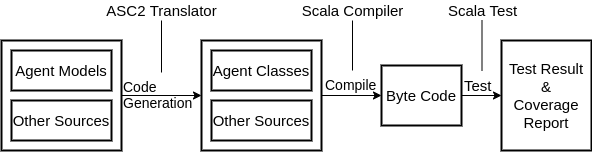
\includegraphics[width=0.80\linewidth]{ch_emas/sbt_proc.png}
  \caption{Compile/Test process of an ASC2 program with sbt}
  \label{fig:sbt1}
\end{figure}

In our approach, we aim to allow the designer to utilize any off-the-shelf testing tool (library, service, etc.) directly into their development chain, even more so to enable the designer to test their program via any standard build chain. 
In the case of the ASC2 framework, its current implementation is based on Scala, and we considered as target build tool \textit{sbt}\footnote{\url{https://scala-sbt.org/}}, which enables us to also use JVM/Scala testing libraries like \textit{JUnit} or \textit{ScalaTest}. We have then developed a sbt plugin\footnote{\url{https://github.com/mostafamohajeri/sbt-scriptcc}} that %when enabled in a project
---as part of the compile task---iterates over the scripts written in AgentScript DSL in the project sources and uses the AgentScript Translator to generate Scala implementations of the agents. Code generation is a standard part of build tools like sbt or maven, therefore, the generated sources are also managed by the build tool and are immediately available to rest of the project. The general overview of the \textit{Compile/Test} cycle of an agent-based system developed via ASC2 and built by sbt is presented in figure \ref{fig:sbt1}. Note that this process is fully automated by sbt. 


A MAS of this type can be started in two ways. After bootstrapping it as an empty instance of the MAS infrastructure, the designer can either use configuration files (e.g. JSON) to specify the agents of the system or alternatively, use lower-level code (e.g. Scala/Java) to manually spawn agents via their respective class in the generated code. In this work, we preferred the latter approach, as it provides better control over the test scenarios.

To complete our Compile/Test process, in addition to the \textit{ScalaTest} library, we also used the \textit{Akka Testing} library: at run-time, ASC2 agents are essentially Akka actor micro-systems and this library provides many convenient tools for testing actors. Both libraries are used out of the box and no modifications have been done to adapt them to the framework. With this configuration, each scenario to be verified can the written as a test suite in ScalaTest to test whether one or multiple agents behave as expected.

\begin{listing}[!tb]

\centering
\begin{minted}[linenos]{prolog}
+!init(W) : W > 1 =>
    Nbr = "worker" + 
        ((#name.replaceAll("worker","").toInt mod W) + 1);
    +neighbor(Nbr).

+!token(0) =>
    #coms.achieve("master", done).

+!token(N) : neighbor(Nbr) =>
    #coms.achieve(Nbr, token(N - 1)).
\end{minted}
\vspace{-5pt}
    \caption{Token ring \texttt{worker} script in AgentScript DSL}
    \label{lst:script_1}
\vspace{-5pt}
\end{listing}

\section{Illustrative Example}
\label{sec:example}
To illustrate an application of our testing approach we consider a MAS constructed around a Token Ring system, commonly used in both distributed systems and MAS \cite{MohajeriParizi2020,Cardoso2013}. This system consists of one master agent and $W$ worker agents; at the start of the program the master sends an $init(W)$ message to all worker agents to inform them of the total number of the workers in the ring, each worker upon receiving this message finds its neighbor, forming a closed ring. Then, $T$ tokens are distributed among the workers, each token has to be passed $N$ times in the ring formed by workers. When all $T$ tokens have been passed $N$ times and this was reported to the master, the program ends.

% \begin{comment}

% A token ring MAS program should:
% \begin{itemize}
%     \item create one master and $W$ number of workers;
%     \item the master sends a $init(W)$ event to all workers, where $W$ is the number of workers in the ring; then it distributes all the tokens $1\leq i \leq T$ with a counter $N$ to workers;
%     \item each worker that receives $init(W)$ should determine its neighbor in order to form and to complete its ring;
%     \item when a worker receives a token it subtracts from the token's counter and sends it to its neighbor unless the token's counter has reached $0$ in which case it sends a $done$ message to the master;
%     \item the program finishes when all $T$ tokens have been passed listing $N$ times and the master have received $T$ number of $done$ messages
%  \end{itemize}
 
%  \end{comment}

\subsection{Unit/Agent Testing}
We will focus in particular on the script of the worker agents shown in listing \ref{lst:script_1}. We perform the tests taking the standpoint of a \textit{whitebox} test engineer, meaning that we test the script of the agent knowing its internal workings; nevertheless, the tests are still performed externally, we do not modify the script in order to test it\footnote{\url{https://github.com/mostafamohajeri/agentscript-test}}.

\subsubsection{Testing Successful Scenarios}
By viewing the script in listing \ref{lst:script_1}, we can see that the agent has a total of 3 plans for 2 separate goals. Theoretically, we need at least 3 tests to cover the successful execution of all the plans. However, while the success criteria for plans is simple (completion of execution), achievements of goals can be more complicated and the testing framework needs to provide the flexibility to define them. The success criteria for the \texttt{init(W)} and \texttt{token(N)} goals are quite different. In the latter the expected behaviour in both plans is an observable event, i.e. a certain \texttt{achieve} message sent by the agent to another specific agent. In the former case there is no observable behavior and the success criterion is a specific update of the agent's belief base.





\begin{listing}[!tb]
\centering
\begin{minted}[linenos]{scala}
class TokenRingWorkerSpec extends ... {

  val mas = new MAS()
  val verifiableBB  = new BeliefBase()
  val mockedMaster = testKit.createTestProbe[IMessage]()
  val mockedNeighbor = testKit.createTestProbe[IMessage]()
  val worker

  override def beforeAll(): Unit = {
    mas.registerAgent(new worker(bb = verifiableBB), name = "worker1")
    mas.registerAgent(mockedMaster, name = "master")
    mas.registerAgent(mockedNeighbor, name = "worker2")
    worker = mas.getAgent("worker1")
  }

  "A worker agent" should {
    "have its neighbor in its belief base after `!init(N)`" in {
      worker.event(achieve,"init(50)").send()
      mockedMaster.expect(GoalAchievedMessage())
      assert(verifiableBB.query("neighbor(worker2)") == true)
    }

    "send a `!done` to master on `!token(0)`" in {
      worker.event(achieve,"token(0)").send()
      mockedMaster.expect(event(achieve,"done").source(worker))
    }

    "send a `!token(N-1)` to its neighbor on `!token(N)`" in {
      worker.event(achieve,"token(10)").send()
      mockedNeighbor.expect(event(achieve,"token(9)").source(worker))
    }
  }
}
\end{minted}
\vspace{-5pt}
    \caption{Test suite for the \texttt{worker} agent}
    \label{lst:test_1}
\vspace{-5pt}
\end{listing}

The test specification we used for the worker agent can be seen in listing \ref{lst:test_1}. In line 3 an empty MAS object is created. The criterion of success for \texttt{init(W)} plan depends on the agent's beliefs, therefore we need to be able to verify the internal state of agent's belief base. First we create an instance of \texttt{BeliefBase} class (line 4) and when the agent under test (\texttt{worker1}) is being instantiated (line 10), this object is injected in the agent as its belief base; with this approach at any point in the tests we can simply access the agent's beliefs to query them for verification purposes or even modify the agent's belief base for setting up test scenario states.

Only one agent (\texttt{worker1}) is under test and the other agents present in the suite can be mocked. As ASC2 agents are actor micro-systems, an agent can be mocked by a single actor. In lines 5 and 6, two \textit{probe} actors are created to be the stand-ins for the master agent and (\texttt{worker1})'s neighbor in the tests and they are then registered to the system (lines 11 and 12). This type of mocking gives us the ability to verify all the interactions that the agent under test may have had with these probe actors.

%Note that ScalaTest (or any other testing tool) already provides convenient interface functions like \texttt{beforeAll} to set up a test.

The rest of the test suite contains 3 tests, in the first test in line 18 a goal event \texttt{init(50)} is sent to the \texttt{worker1} agent and it is expected that after this goal is achieved (line 19), the belief base of the agent contains the belief defined by the term \texttt{neighbor(worker2)} which is verified in line 20. In the next test, a goal message \texttt{token(0)} is sent to the agent (line 24) and then it is verified that the agent sends a \texttt{done} message to the master (line 25). The final test follows the same pattern by sending a goal message \texttt{token(10)} (line 30) and the verification includes a \texttt{token(10-1)} message to its neighbor (line 30). Note that in all the tests, the messages sent to the \texttt{worker1} agent do not specify any source, this is because in the script in listing \ref{lst:script_1}, the source of the messages is not checked meaning it is not necessary to specify the source. As these tests are written in a standard testing library, build tools such as \textit{sbt} can execute them in their build chain. By running the tests in the sbt shell we are able to see the output presented in listing \ref{lst:result_1} that indicates our program has passed this test.

\begin{listing}[!h]
\begin{Verbatim}[fontsize=\small]
[info] A worker agent should
[info] - have its neighbor in its belief base after `!init(N)`
[info] - send a `!done` to master on `!token(0)`
[info] - send a `!token(N-1)` to its neighbor on `!token(N)`
...
[info] All tests passed.
\end{Verbatim}
\vspace{-5pt}
    \caption{Output of the \texttt{worker} agent test suite}
    \label{lst:result_1}
\vspace{-5pt}
\end{listing}




\subsubsection{Testing Failure Scenarios}
Successful executions are only a part of the full story. Indeed, in software testing it is acknowledged that covering \textit{failures} is both more important and challenging, and thus requires more critical thinking by the test engineer \cite{ArtOfTesting}. Interestingly, failure tests are especially important in agent-based programming because failing under certain conditions may sometimes be the correct behavior for an agent. 

Two failure tests are presented in listing \ref{lst:test_2}. The first test sends a \texttt{init(W)} goal message to the agent with \texttt{W=-1} (line 3) but the first plan is applicable only for \texttt{W > 1} and the expected behavior of the agent in this situation is a failure which is verified by expecting a \texttt{NoApplicablePlan} message. In the second test, a goal message \texttt{unknown} is sent to the agent (line 8) for which the agent does not have any plans and it should reply with a \texttt{NoRelevantPlan} (line 9). Note that failure of a goal is not only reflected by the absence of an applicable plan or more generally failure in execution of a plan; similar to the success scenarios, the designer can define any other arbitrary criteria for a failure scenario.

\begin{listing}[!tb]
\centering
\begin{minted}[linenos]{scala}
"A worker agent" should {
  "send a `NoApplicablePlan()` on `!init(-1)`" in {
    worker.event(achieve,"init(-1)").source(mockedMaster).send()
    mockedMaster.expect(NoApplicablePlan())
  } 
  
  "send a `NoRelevantPlan()` on `!unknown`" in {
    worker.event(achieve,"unknown").source(mockedMaster).send()
    mockedMaster.expect(NoRelevantPlan())
  }
}
\end{minted}
\vspace{-5pt}
    \caption{Failure tests for \texttt{worker} agent}
    \label{lst:test_2}
\vspace{-5pt}
\end{listing}

% This type of failure test, despite being simple, can be a very powerful tool for the designer to reveal the incorrect behaviors of the agent program.

Although we acknowledge that testing an agent program for every possible failure can easily become an infeasible task \cite{Winikoff2015,Winikoff2017}, certain failures may be particular important for the designer to test, therefore there is value in enabling this possibility.

\subsection{Coverage}

% Continuing from the previous section on how we use off-the-shelf testing libraries to write tests for ASC, 

We explore at this point whether and how off-the-shelf coverage tools such as \textit{scoverage}\footnote{\url{http://scoverage.org/}} can be used for code coverage analysis of agent programs written in ASC2, considering both statement and branch coverage aspect. To perform this we simply add the scoverage plugin to our project and generate a coverage report.

The coverage report produced for the worker agent by means of the previous tests is presented in Table \ref{tab:coverage}. The \texttt{worker.Agent} row shows the coverage for the internal mechanisms of the agent, like e.g. \textit{event handling}, 
%(excluding the belief base) 
while the other rows show the coverage report for each separate event, as an example, the \texttt{worker.token\_1} refers to an event \texttt{token} in \texttt{worker} agent with 1 parameter. The branch coverage report mainly concerns conditional statements in the generated Scala code of the agent and should be regarded only as informal information about the coverage of the main script.

These results show that our tests indeed covered most of the behaviors that the agent might have. In fact, by exploring the coverage analysis we can see the reason for which the \texttt{worker.token\_1} has less coverage: the missed branch can be explained by the fact that the tests did not include any scenario in which the \texttt{token(N)} plan fails. Also note that while the example script did not contain any sub-goals or conditional statements in the plans, ASC2 Translator generates sub-goal adoptions as function calls and translates conditional statements to their counterpart in the underlying language, therefore, coverage tools like \textit{scoverage} are able to calculate the correct number of covered and total possible branches for deeper goal-plan trees.
\vspace{-5pt}

\setlength{\tabcolsep}{0.5em} % for the horizontal padding
{\renewcommand{\arraystretch}{1.1}% for the vertical padding
\begin{table}
    \centering
    \begin{tabular}{lll}
        \toprule
        Component &  Statement Coverage \% & Branch Coverage (Covered/Total) \\
        \midrule
       \texttt{worker.Agent}  &  93.5  & 6/6 \\
       \texttt{worker.init\_1} &  93.5  & 2/2 \\
       \texttt{worker.token\_1} &  80.2  & 3/4 \\ \bottomrule
    \end{tabular}
    \vspace{5pt}
    \caption{Coverage analysis of the \texttt{worker} agent}
    \label{tab:coverage}
    \vspace{-10pt}
\end{table}
}

\subsection{Integration/System Testing}
%Integration testing refers to the activity of verifying that different modules of a software system work together in a correct way. In practice, software integration tests often are done on modules developed by different teams located in different repositories and it is important that testing tools support this type of setups. Furthermore, in the MAS testing community there are conceptual guidelines on how to decide what the modules of a systems are \cite{Moreno2009}. We continue with an integration test setting that aligns the theoretical aspect of MAS testing with the practical requirements of software testing.

%The integration test suite that verifies a system consisting of the previously mentioned \texttt{worker} agent hosted on one repository and a \texttt{master} agent hosted on another. The integration test project will need to fetch both projects prior to running the test suite.  

%The MAS testing community provides conceptual guidelines on how to decide what the modules of a systems are \cite{Moreno2009}. We will follow these guidelines for giving an example of integration test suite,

Even following the guidelines on categorizing different levels of testing in MAS \cite{Moreno2009}, there is no definite technical distinction in place. Typically test libraries provide mechanisms such as annotations for the designer to label test suites with its (their) related level(s) to orchestrate their execution. As illustration, we consider an integration test to verify a token ring MAS system consisting of the previously mentioned \texttt{worker} agents and a \texttt{master} agent. The test suite is reported in listing \ref{lst:test_3}.

\begin{listing}[!tbh]
\centering
\begin{minted}[linenos]{scala}
class TokenRingIntegrationSpec extends ... {
  
  //a communication layer that records a trace of the interactions
  object recordedComs extends AgentCommunicationsLayer { ... }

  val token_pattern = "token\\([0-9]+\\)".r
  val done_pattern = "done".r

  "A token ring MAS with W = 100, T = 50 and N = 4" should {
    "have 250 `token(X)` and 50 `done` message" in {
      // create the agents
      mas.registerAgent(new worker(coms = recordedComs), num = 100)
      mas.registerAgent(new master(coms = recordedComs), name = "master")
      // invoke the system
      mas.getAgent("master").event(achieve, "start(50,4)").send()
      // verify the interactions
      watchdog.expectTerminated( mas, 10.seconds )
      assert(recordedComs.trace.count(token_pattern.matches) == 250)
      assert(recordedComs.trace.count(done_pattern.matches) == 50)
    }
  }
}
\end{minted}
\vspace{-5pt}
    \caption{Integration test suite for the token ring system}
    \label{lst:test_3}
    \vspace{-5pt}
\end{listing}


The test will be centered around the interactions between agents and the state of the system in a specific setting of our token ring. The token ring is defined with 100 \texttt{worker} agents and 1 \texttt{master} agent (lines 12-13), and, to be able to verify the exhibited interactions, we use dependency injection to initialize all the agents by means of an overridden instance of the communication layer (line 4), created to record every message passed in the system into a list. 

To invoke the system, a \texttt{start(T,N)} is sent to the \texttt{master} agent (line 15). We are interacting with the \texttt{master} from a \textit{black box} perspective: although the event \texttt{start(T,N)} is exposed, the internal mechanisms of this agent are assumed to be unknown.

Three criteria are verified for this system. Firstly, we consider a system level performance based criteria as we expect the system to be terminated under 10 seconds (line 17). Next, we use two known expectations from a token ring system to verify the correct execution of the system: at the end of execution, there should be (a) $T$ number of \texttt{done} messages and (b) $T \times (N + 1)$ number of \texttt{token(X)} messages in the trace. The interaction verification statements are presented respectively in lines 18-19. Recalling the flexible definitions of testing levels, note that these integration/system test could be considered from the perspective of \texttt{master} agent as a unit/agent level test possibly with mocking the \texttt{worker} agents. Similar to previous tests, running this suite via sbt yields the output in listing \ref{lst:result_2}.

\begin{listing}[!h]\vspace{-10pt}
\begin{Verbatim}[fontsize=\small]
[info] A token ring MAS with W = 100, T = 50 and N = 4 should
[info] - have 250 `token(X)` and 50 `done` message
...
[info] All tests passed.
\end{Verbatim}
\vspace{-5pt}
    \caption{Output of the token ring integration test suite}
    \label{lst:result_2}
\end{listing}


\vspace{-20pt}
\subsection{Continuous Integration}
The proposed approach for testing can be easily combined with online CI services. This process generally includes utilizing source repositories like Github\footnote{\url{https://github.com/}}, CI services like TravisCI and code analysis services like Coveralls\footnote{\url{https://coveralls.io/}}. The only step needed to set  the CI cycle for an ASC2 project is to configure the source repository of the project in a way that the automated CI cycle is triggered on every \texttt{push} to the repository. This can be done by adding a configuration file that provides information for the CI service how to compile and test the project via sbt.%, and on how to register the project on the relevant CI service. 

Following this method, a MAS project does not need to be only located in a single source repository. For instance, different types of agents can be developed in different projects by separate teams and only be used as dependencies in the development of the system. We believe this is an interesting practical innovation, improving the scalability of MAS projects with respect to their development. 


An overview of an example CI process for the token ring is presented in Figure \ref{fig:ci} in which the sources of \texttt{worker} and \texttt{master} agents are located in separate repositories, and a third token ring repository uses them as dependencies. When the system designer pushes the project to the repository, the CI service fetches the source and compiles and tests it via sbt and records the results\footnote{\url{https://travis-ci.com/github/mostafamohajeri/agentscript-test}}. Then, the code coverage report is committed to the code analysis service\footnote{\url{https://coveralls.io/github/mostafamohajeri/agentscript-test}}.


\begin{figure}[t!]
  \centering
  \hspace{-5pt}
  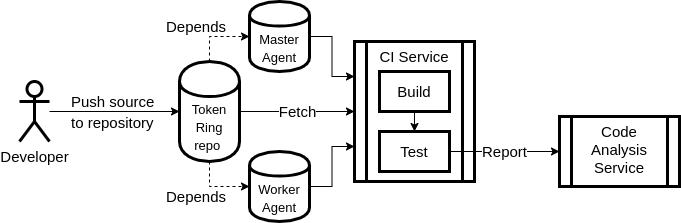
\includegraphics[width=1\linewidth]{ch_emas/ci.png}
  \caption{Continuous integration applied on a Token ring program whose master and worker agent scripts are located on other repositories.}
  \label{fig:ci}
  %\Description{Actor-based architecture of an agent}
\end{figure}

% AgentScript is JVM based so in principle MCAPL should work on it
% Test Generation can be done with this approach

\section{Discussion and Future Developments}
\label{sec:discussion}
%While the successful execution of the plans share the same criteria: completion without exceptions, for an intelligent agent the criteria for the achievement of the respective goals may be different and critically the testing approach for such agents allows for flexible definitions of success criteria.

Despite the critical points/observations concerning MAS testing raised in the literature, in this chapter we % break a lance 
provide several support arguments for using  mainstream testing tools for MAS and agent-based programming, by means of a concrete use case. We implemented a multi-agent system reproducing a token ring benchmark with the framework ASC2, and then we run tests (success, failure, coverage) at unit/agent level as well as at integration/system level. 

%The bottom-line about the applicability of such a method is that the used agent and MAS programming framework needs to be compatible with mainstream software build processes. By satisfying this requirement (as in the case of ASC2), one can utilize development tools and services available to other programming languages for testing, coverage analysis and CI. Our experience in attempting to integrate agent-based development with concurrent development conducted by other programming methods in the context of data-sharing infrastructures made us clear the necessity and urgency of this innovation. We do not claim here that all application domains of MAS require such an operational constraint, but we observe that there are applicative niches that can greatly benefit of  cross-compilation solutions.



At the unit and agent level (unit testing) we performed tests concerning events, plans and goals. The somehow unexpected result of the experiment is that such an approach does not neglect the theoretical complexity of BDI agents but it truly offers a complementary tool for their development. We were able to test successful (plan) completions, internal states and the belief base, failures, and fine-grained interactions. 
These possibilities can be seen as offering  constructs mapping e.g. to declarative and procedural goals in BDI agents \cite{Winikoff2002}: the designer can define the achievement/failure of a goal not only in terms of completion/exception of a plan, but also as determined by any arbitrary indicator internal or external to the agent. This showed that testability of agent programs defined in a framework is closely related to the design choices of that framework. 
% t 

At the integration/group and system/society level (integration testing) we performed tests with simple verification criteria, but these criteria can easily be extended to more sophisticated and realistic interaction analysis and verification methods developed by the MAS community \cite{Botia2006}. Additionally, we illustrated how the proposed approach enables the MAS designer to take advantage of continuous integration (CI) services without extra effort. This is particularly important for MAS designers that require to integrate and test their work continuously with other projects.

There is an additional benefit of using mainstream test tools for BDI agents, and especially for frameworks that are based on higher-level logic-based DSLs. Those frameworks generally map primitive actions to constructs specified in a lower-level programming language like Java. By using a testing process compatible with both higher level models and lower level implementations, the testing process can be more efficient and seamless for the designer specially if the agent models are only a part of a project that includes other computational entities that are being developed alongside the agents. 

An issue in using mainstream test libraries for a BDI framework with a logic-based DSL is the disparity between the high-level agent DSL and the lower-level language used for the tests. This can be addressed by either developing approaches to write tests in the high-level DSL or creating interfaces for the low-level language to enable the test engineer to implement tests at a proper level of abstraction. In this work we have taken the latter approach.
%In this work we used the ASC2 agent programming framework to present our approach, 
The intuition behind this choice was that frameworks based on cross-compila-tion \cite{Astra,Sarl} produce source codes that can be directly integrated within standard build tools.

Can our results be generalized to other agent programming frameworks?
Motivated by the success of works like AJPF/MCAPL \cite{Dennis2016} that provides model checking for multiple BDI frameworks, as a future study we intend to explore how to apply this approach to a wider range of MAS frameworks.
Yet, we can already trace some higher-level considerations.
%This raises the question:
The answer, at the unit/agent level, depends on compilation and the execution model of those frameworks. For frameworks like Jade and JS-son \cite{Kampik2020}, that use mainstream programming languages to define agents, these tools should be compatible out of the box with minor effort \cite{Khamis2013}. For cross-compilation-based frameworks like Astra \cite{Astra} and ASC2 \cite{MohajeriParizi2020} it is only the matter of tooling (e.g. build tool plugins) to allow them to use mainstream testing tools. For interpreter-based frameworks like Jason \cite{Bordini2005} and GOAL \cite{Hindriks2009a}, because they require their own dedicated reasoning engines and execution environment, %which are not recognizable by the mainstream tools and developing tools to bridge them into mainstream testing tools
testing via such tools may prove to need more work and possibly modifications to the framework. This issue may be not so problematic, as there are already many works that propose dedicated testing and debugging approaches for interpreter-based frameworks \cite{Koeman2016}.
%be impractical and 
%however, typically interpreter-based frameworks provide their own dedicated testing/debugging approaches \cite{Koeman2016}.

At the integration and system level, and also with respect to compatibility with CI services, generally externalized to the execution of the tested entity, we believe it is possible to consolidate other frameworks regardless of their compile/interpret model. This could lead to seamless integration testing of systems defined in each framework with mainstream software testing tools or dedicated ones.

In perspective, our overarching research concerns socio-technical and complex multi-domain infrastructures; we believe that Agent-Oriented Software Engineering can be a powerful technical tool with robust theoretical foundations for designing, modelling, implementing and testing such systems.  Enhancing their development cycle goes with a seamless integration of multi-agent systems into modern infrastructures. This is a critical requirement to utilize the full potential of MAS in a real production-level setting. 

\chapter{Introducing Norms to Agents: Normative Advisors}
\label{ch:normative_advisors}
\textcolor{red}{ABSTRACT REWRITE and SOME TONE CHANGE IN THE BODY} This chapter introduces a modular architecture for integrating norms in autonomous agents and multi-agent systems. As the the interactions between norms and agents can be complex, this architecture utilizes multiple programmable components to model concepts such as adoption of multiple personal and/or collective possibly conflicting norms, interpretation and qualification between social and normative contexts, possibility of intentionally (non-)compliant behaviors and resolving conflicts between norms and desires (or other norms). The architecture revolves around \emph{normative advisors} that act as the bridge between intentional agents and the institutional reality. As a technical contribution, a running implementation of the architecture is presented based on the ASC2 (AgentScript) BDI framework and eFLINT norm reasoner. 


\section{Introduction}
Designing software agents that can reason with norms---technical instances of \emph{normative agents}---requires evidently having a suitable computational model for reasoning with norms. This is a challenging task because norms are more than a set of formal rules extracted from a legislative text: they emerge from multiple sources with different degrees of priority, they require interpretation to be encoded and qualification to be applied within a social context. Furthermore, they continuously adapt, in both expression and application~\cite{Boella2014APractice}. 

Previous proposals to embed norms in multi-agent-systems (MAS) have focused on extending the agent architecture (usually based on beliefs-desires-intentions, or BDI) to allow for forms of normative reasoning \cite{Dignum2002MotivationalNorms,Broersen01theboid,Tufis2017,Criado2010TowardsCompliance}. Two general approaches can be identified in the literature. One can encode norms as facts, and axiomatize normative reasoning with dedicated rules, to leverage the inferential engine provided with the agents; in this case, no modification needs to be applied to normative agents compared to non-normative agents. In contrast, in frameworks like BOID~\cite{Broersen01theboid} or B-DOING~\cite{Dignum2002MotivationalNorms}, explicit normative components like obligation (O) are considered to play a role in the decision-making cycle, requiring a modification of said cycle. In both cases, the agent is considered as a unity from an execution point of view: the agent script is a program, usually interpreted, and its internal reasoning cycle executed by a single thread. This work starts from the observation that this constraint is a rather strong one, not needed, and not always the most suited. Rather than an event-based reactive architecture based on a single event-queue and scheduling, individual agents may be each implemented as a system of concurrent actors, provided with some form of organization (e.g. event dispatching) and interaction mechanism (e.g. messaging).% Clearly, the overhead of complexity required for setting up a correct coordination amongst computational units, and for enabling and/or performing debugging, does not provide a good case for such construction. 

Normative agents offer a context in which this way of design gains more viability, for several reasons. On \textit{content} level, multiple normative sources may be concurrently relevant, and/or multiple interpretations of the same normative sources may be available (e.g. retrieved from previous cases), and these may be possibly conflicting. Enabling to maintain those in a modular fashion is a suitable precondition for update/adaptation actions, where norms can be changed on the fly, and agents may decide at run-time e.g. to change the relative priority between normative components. On \textit{method} level, there is still an ongoing debate on what is the most adequate representation model for norms, and on proper methods for normative reasoning (e.g. managing conflicts). Enabling the recourse to external tools, and supporting programmability of the coordination level, greatly empowers modelers/programmers/designers to test and compare different choices. Finally, at \textit{functional} level, most of the knowledge instilled in norms concerns a full social system; only a part is contingently relevant to the agent. Designing the system so that it distributes the inferential load at best (and at need) externally from the decision-making is seemingly the most efficient option.

\paragraph{Contribution}
For these reasons, this work proposes an abstract architecture that encapsulate norms (namely encoded in terms of normative relationships of Hohfeld's framework) in a MAS. The architecture centers around \textit{normative advisors} that can be utilized by (other) agents in the MAS as a sort of council about the institutional state of affairs and normative relations between agents, highlighting the mapping between the social and institutional views of the environment. Agents may resort to personal or to collective advisors, depending on the decentralization constraints set up by the designer.   
%
As a technical contribution, we present a practical implementation of this architecture that relies on the AgentScript BDI framework (ASC2) \cite{MohajeriParizi2020} for programming agents, and norm specification framework eFLINT \cite{VanBinsbergen2020EFLINT:Specifications} for encoding norms. 
%



\paragraph{Related works}
% There are multiple existing works in the literature on this topic. 
The B-DOING framework \cite{Dignum2002MotivationalNorms} explores logical relations between belief, desire, obligation, intention, norms and goals in agents and their interactions like conflicts and possible appraoches to balance them in agent's behavior. Similarly, the BOID architecture \cite{Broersen01theboid,Pandzic2022BOID} proposes a belief, obligation, intention and desire architecture with a feedback loop to take the effects of actions before committing to them. These studies (and many others, e.g., \cite{Deljoo2018APlaces,Tufis2017}) propose extensions to the BDI architecture to add (regulative) norms as part of the agents' mind and to resolve conflicts with pre-defined rules as part of the agent's reasoning cycle.


The normative BDI architecture presented in \cite{Criado2010TowardsCompliance} proposes different contexts for an agent: mental, functional and normative contexts, plus ``bridge rules'' between them. Their approach aims at creating maximally compliant agents and focus on solving conflicts between norms at the time of adoption by using pre-defined conflict resolution rules. The work presented in \cite{Cardoso2021ImplementingBDI} propose an approach for ethical reasoning in MAS by programming \textit{ethical governors}. Their method is close to ours in the sense that they also take advantage of extra agents in a MAS, but they focus on machine ethics used in the decision-making of one agent.


\paragraph{Structure of the document}
Section~\ref{sec:background} gives background on the core components that the proposal uses, providing some detail on the AgentScript/ASC2 and eFLINT frameworks. Section~\ref{sec:framework} lays out the theoretical framework for the proposed architecture, whereas Section~\ref{sec:implementation} describes details of its implementation. Section~\ref{sec:discussion} reflects on the capabilities of our implementation, suggests future directions, and draws connections with related work.


\section{Core components\label{sec:background}}

\begin{figure}[!tb]
    \centering
    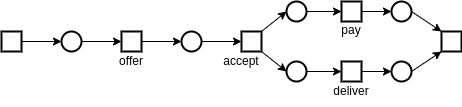
\includegraphics[width=0.5\textwidth]{ch_eumas/sale-drawio.png}
    \caption{Sale transaction as a \textit{Petri net} workflow}
    \label{fig:sale}
\end{figure}
%

To illustrate our approach, we will consider as a running example a marketplace environment consisting of buyer and seller agents. This target domain can be seen as an abstract model of many real-world domains, e.g. data market-places and more in general data-sharing infrastructures, electronic trading infrastructures, etc. The process model of a individual sale transaction---prototypical example of bilateral contract---can be represented as a workflow through a Petri-net, presented in Figure~\ref{fig:sale}. A seller offers a buyer an item for a certain price. If the buyer accepts the offer, then the seller is expected to deliver the aforementioned item to the buyer, and the buyer is expected to pay the seller the agreed upon price (in any order). The workflow is a simplified representation of the normative mechanisms in place during an actual sale transaction. Furthermore, it does not consider the intentional aspects on the agents during the transaction, e.g. based on which desires or goals the agents may be willing to engage in the transaction, as these concepts stay external to norms.
%It does not consider \textit{why} the agents may be willing to engage with the transaction (purpose, on which bases, expectations, etc.), nor the various normative relationships dynamically created along the process in order to guide the coordination between the parties. 
%To capture those, we need to further increase the design granularity of our target system.
%
\subsection{Intentional agents}
The intentional agents defined in this chapter intuitively are implemented in ASC2. 
%\gio{[There are a few things which are not explained of the code. e.g. a couple of words on the initalization of the normative advisor, and more importantly on \texttt{\#achieve}... what does it serve for? Has it any connection with the speech act? I would take one plan rule (e.g. \texttt{+offer}) and explain it in detail. Overall the granularity/size of this paragraph should be similar to the one of eFLINT.]}
Continuing with the example, Listing~\ref{asc:buyer}, presents the script of a buyer agent. The initial beliefs (lines 1-3), initial goals (line 5), and plan rules (line 7 and onwards) are the components of the script. The script is further explained in Section~\ref{sec:scenario}. 

% Intentional agents are generally approached in the computational realm via the \textit{belief-desire-intention} (BDI) model \cite{Rao1995}, % is used as the reference to define intentional agents. 
% %Having its roots in a theory of mind \cite{bratman1987intention}, the BDI model has been 
% %investigated in the literature as basis 
% to specify computational agents acting in dynamic environments with rational behavior.
% % uses taxonomies that are used typically to address human behaviour to describe agents.
% The BDI model refers to three human mental attitudes % used to describe human behavior 
% \cite{bratman1987intention}: \textit{beliefs} are the factual and inferential knowledge of the agent about itself and its environment; \textit{intentions} are the courses of action the agent has committed to; \textit{desires}, in their simplest form, are objectives the agent wants to accomplish. In practice, BDI agents also include concepts of \textit{goals} and \textit{plans}. Goals are concrete desires, plans are abstract specifications for achieving a goal, and intentions then become commitments towards plans. Multiple programming languages and frameworks have been introduced to operationalize the BDI model, such as AgentSpeak(L)/Jason~\cite{RaoAS1996,Bordini2005}, 3APL/2APL~\cite{Dastani2007}, Astra~\cite{Dhaon2014} and AgentScript/ASC2~\cite{MohajeriParizi2020}.
%
\begin{listing}[!h]
\begin{minted}[linenos,fontsize=\small]{prolog}
needed_item("Book1").
fair_price("Book1", 5).
have_money(10).

!init(#sale_advisor.getClass, "sale.eflint", "BuyerAdvisor").

+!init(AgentType,EFFile,Name) => 
    #spawn_advisor(AgentType, EFFile, Name).

+offer(I ,P) =>
    #achieve("BuyerAdvisor", perform(offer(Source, Self, I, P)));
    !consider_buying(Source, I ,P).
    
+!consider_buying(Seller, I, P) : 
  needed_item(I) && fair_price(I, FP) &&
  P =< FP && have_money(M) && M >= P =>
    #tell(Seller, accept(I, P));
    +pending(accept(I, P)).

+acknowledge(accept(I, P)) : pending(accept(I, P)) =>
    -pending(accept(I, P));
    #achieve("BuyerAdvisor", perform(accept(Self, Buyer, I, P))).

+duty_to_deliver(Seller,Buyer,I) : 
    Source == "BuyerAdvisor" && Buyer == Self => 
        +expected_delivery(Seller,I).
    
+delivery(Sender, I) : expected_delivery(Sender, I) =>
    -expected_delivery(Sender, I);
    #achieve("BuyerAdvisor", perform(deliver(Sender, Self, I)).

+duty_to_pay(Buyer, Seller, P) :
    Source == "BuyerAdvisor" && Buyer == Self  =>
        !pay(Seller, P).
    
+!pay(Seller, P) : have_money(M) && M >= P => 
    #pay(Seller, P);
    #achieve("BuyerAdvisor", perform(pay(Self, Seller, P)).
    
+!pay(Seller, P) => ... ALTERNATE APPROACH TO PAYMENT ...
\end{minted}
\caption{Buyer agent script as ASC2 program}
\label{asc:buyer}
\end{listing}


%In this work, the AgentScript BDI framework is used to implement both intentional agents and normative advisors. 
%

% \subsubsection{AgentScript/ASC2 Agent Framework}
% The ASC2 agent programming framework is composed of the AgentScript domain-specific language (DSL) and a cross-compiler. The cross-compiler translates agent programs written in the AgentScript to Scala executable programs utilizing the Akka actor-oriented framework, meaning at run-time, each agent is a composition of multiple actors. The AgentScript DSL has a very close syntax to AgentSpeak(L), % and includes some of the extensions provided by Jason.  
% % \gio{[I would add a little bit more of the AgentScript framework, i.e. ASC2 as cross-compiler to Akka actors.]}
% consisting of initial beliefs and goals, and, plans. Initial beliefs are a set of Prolog-like facts or rules that define the first beliefs the agent has,
% and, initial goals designate the first intentions to which the agent commits. Plans are potentially non-grounded reactive rules in the form of \mintinline{text}{ E : C => F }, where \mintinline{text}{E} is the head of the plan which consists of a trigger and a predicate, the trigger can be one of \mintinline{text}{+!,-!,+,-,+?} respectively used for achievement goals, failure (of) goals, belief-updates (assertion, retraction) and test goals. The expression \mintinline{text}{C} is the context condition that can be any valid Prolog expression, and, \mintinline{text}{F} is the body of the plan that consists of a series of steps that can include belief-updates (\asc{+belief,-belief}), sub-goal adoption (\asc{!goal}), primitive actions  (\mintinline{text}{#action}) which may be any arbitrary method on program's class path, variable assignments,  and control flow structures %(CFS) 
% (loops and conditionals).
% %that map different internal events (e.g, \textit{goal adoption}, \textit{belief-update}) or external events (e.g, \textit{message reception}, \textit{perception}) to a sequence of executable steps called the \textit{plan body} which the agent has to perform in response to the event. 
% It is said that a plan is \textit{relevant} for an event \mintinline{text}{G} iff the event-type of \mintinline{text}{G} matches with the trigger and the content of \mintinline{text}{G} matches with the predicate of \mintinline{text}{E}. Furthermore, a relevant plan is \textit{applicable}, iff \mintinline{text}{C} is a logical consequence of agent's belief-base. When an agent receives an event, as a reaction, after finding the relevant, and then applicable plans, it will use a selection function to choose a plan to execute as an intention. This process is typically called \textit{planning} in BDI agents.
% %





\subsection{Norms and Normative (Multi-Agent) Systems}
\label{sec:back:norms}
% In this paper we follow Gibbs' definition -- widely used in especially the normative MAS community -- and say that 
Following Gibbs, we consider norms as ``a collective evaluation of behavior in terms of what it ought to be; a collective expectation as to what behavior will be; and/or particular reactions to behavior, including attempts to apply sanctions or otherwise induce a particular kind of conduct''~\cite{Gibbs1965Norms:Classification.}. This definition is relevant to our purposes as it gives primacy to action (rather than to situations, as in most deontic logic accounts). In the context of multi-agent systems, and even more of in MAS, an action-centered approach is intuitively more suitable, as actions are the only means agents have to intervene on the environment, and by which determine normative consequences.

% %
% In particular, we take an action-oriented approach in which actions may be permitted, may have normative consequences, may be obliged, and may be the response to violations (of prohibitions or obligations).
% %
% For example, in our approach, an actor $P$ may have given a duty to an actor $A$ to complete a certain task before a deadline, and an actor $E$ may have the power to (on behalf of $P$) respond to $A$'s violation of the duty by sanctioning $A$. 
% %
% This is in line with the Hohfeldian framework in which the potestative power-liability positions and the deontic duty-claim positions describe normative \emph{relations} between actors, i.e. between the holder of a power and the actor affected by the power (liability) and between the holder of a duty and the claimant to the duty being satisfied~\cite{hohfeld1917fundamental}.

\paragraph{Categories of Norms}
Norms are traditionally distinguished between \textit{regulative} and \textit{constitutive} norms~\cite{Searle1969,Boella2004RegulativeSystems,Sileno2015}.
%
Regulative norms regulate behaviors that exist independent of the norms and are generally prescribed in terms of \textit{permissions}, \textit{obligations} and, \textit{prohibitions} (e.g. traffic regulations).
%
Constitutive norms determine that some entity (e.g. an object, a situation, a certain agent, a certain behaviour) ``counts as'' something else, creating a new institutional entity that does not exist independently of these norms. (for example, the concept of marriage or money as a legal means of payment). The concept of institutional power is particularly relevant in the context of constitutive norms, as it is used to ascribe institutional meaning to  performances (e.g. raising a hand counts as a bid during an auction). A conceptual framework that instead contains both deontic and potestative dimensions is the one proposed by Hohfeld \cite{hohfeld1917fundamental}, whereas deontic logics, although much more popular, by definition focuses on regulative norms.

%
%These norms are studied less in the normative MAS literature. 
%Nevertheless, there are multiple works in the literature that propose guidelines and definitions for design, utilization, analysis and evaluation of normative MAS \cite{Balke2013NormsConcepts,}.
% \cite{Boella2006IntroductionSystems}
% \cite{Boella2001TheFramework}
% \cite{Boella2009NormativeSystems}
% \cite{Boella2014APractice}
% \cite{Balke2013NormsConcepts}

\subsubsection{Normative systems}
%
The term normative system can be applied to a system of norms, and a multi-agent system guided by norms. Our work builds upon the second standpoint, and more precisely, we apply the so-called \textit{normchange} definition of normative MAS system by Boella et al.~\cite{Boella2006IntroductionSystems}: %and say that 
``a multi-agent system together with normative systems in which agents on the one hand can decide whether to follow the explicitly represented norms, and on the other the normative systems specify how and in which extent the agents can modify the norms''.
%
This definition does not assume any particular inner workings of the agents except that they should be able to somehow \textit{decide} whether to follow the norms or not and they should be able to \textit{modify} them.
%
Furthermore, there is no assumption about the representation of the norms, except that they should be \textit{explicit} (i.e. a `strong' interpretation of the norms~\cite{Boella2009NormativeSystems}) and \textit{modifiable}. 
%


% in this paper, we discuss how to integrate them as the basis for normative (multi-agent) systems. 

% \subsection{Normati

\subsubsection{The eFLINT norm language}
\label{sec:back:eflint}
%
The eFLINT language is a DSL designed to support the specification of (interpretations of) norms from a variety of sources (laws, regulations, contracts, system-level policies such as access control policies, etc.) ~\cite{VanBinsbergen2020EFLINT:Specifications,binsbergen2021b}.
%
The language is based on normative relations proposed by Hohfeld \cite{hohfeld1917fundamental}. 
The type declarations introduce types of \textit{facts}, \textit{acts}, \textit{duties} and \textit{events}, which together define a transition system in which states---knowledge bases of facts---transition according to the effects of the specified actions and events.
%
The transitions may output violations if an action triggered a transition with unfulfilled preconditions (e.g. only sellers can make offers) or if any duties are violated in the resulting state\footnote{In eFLINT, a permitted act may result in changes to normative positions and that the ability to trigger these changes constitutes a power; therefore act frames can be seen as specifying at the same time powers and permissions, and, absence of powers map to prohibitions (as e.g., in access control methods). Other computational frameworks based on Hohfeld propose a more explicit separation between deontic and potestative categories \cite{Sileno2022}. 
}.


% \footnote{\gio{The current version of eFLINT takes the design choice that a permitted act may result in changes to normative positions and that the ability to trigger these changes constitutes a power; therefore act frames can be seen as specifying at the same time powers and permissions, so absence of powers map to prohibitions (as e.g. in access-control methods). Other computational frameworks based on Hohfeld maintain a stricter separation between deontic and potestative categories, e.g. \cite{Sileno2022}.}. 
% }

% concepts of powers and duties and emphasizes the importance of normative relations.
%
\begin{listing}[!ht]
  \centering
\begin{minipage}{1\textwidth}
  \centering
\begin{tcolorbox}[left=2pt,right=2pt,top=2pt,bottom=2pt,arc=0pt,
                  boxrule=0pt,toprule=1pt,
                  colback=white]
\begin{minted}[fontsize=\footnotesize,linenos]{haskell}
// fact definitions
Fact buyer 
Fact seller
Fact item
Fact price Identified by Int 

// act-type definitions
Act offer Actor seller Recipient buyer
  Related to item, price
  Holds when seller
  Creates 
    accept(buyer, seller, item, price)

Act accept Actor buyer Recipient seller
  Related to item, price
  Creates 
    pay(buyer, seller, price),
    duty_to_pay(buyer, seller, price),
    deliver(seller, buyer, item),
    duty_to_deliver(seller, buyer, item)

Act pay Actor buyer Recipient seller
  Related to price
  Terminates 
    duty_to_pay(buyer, seller, price)

Act deliver Actor seller Recipient buyer
  Related to item
  Terminates
    duty_to_deliver(seller, buyer, item)

// duty-type definitions
Duty duty_to_pay 
  Holder buyer
  Claimant seller
  Related to price

Duty duty_to_deliver
  Holder seller
  Claimant buyer
  Related to item
\end{minted}
\end{tcolorbox}
\end{minipage}%
\caption{eFLINT Specification for \textit{Sale Transaction} norms}
\label{listing:eflint}
\end{listing}


%
Listing~\ref{listing:eflint} shows an eFLINT specification for our running example.
%
The \texttt{Actor} and \texttt{Recipient} clauses and \texttt{Holder} and \texttt{Claimant} clauses of act- and duty-type definitions establish constructs mapping to Hohfeldian power-liability and duty-claim relationships.
%
The \texttt{Creates} and \texttt{Terminates} clauses describe the effects of actions when performed, enabling reasoning over dynamically unfolding scenarios.
%
An instance of \asc{offer} can be performed without any pre-conditions and it holds when there is a \asc{seller} instance. 
%
The act \asc{accept} is only available after an offer: accepting a non-existing offer is considered a violation of the power to accept offers.
%
Acceptance of an offer creates the two act instances \asc{pay} and \asc{deliver} which can be performed in any order.
%
The duties express that the \texttt{pay} and \texttt{deliver} actions are expected to be performed by their respective holder after they are created as part of the \texttt{accept} action.
%
As described in Listing~\ref{listing:eflint}, no violation conditions are associated with the duties.
%

% The eFLINT language has features that make it particularly suitable for the purposes of this work.
% %
% %Firstly, 
% Specifications in eFLINT are adaptable, owing both to the modular nature of specifications and to the ability to replace and extend existing declarations. 
% %
% The language allows programs to be developed incrementally by submitting code fragments in a Read-Eval-Print-Loop interpreter, a computational notebook or as part of an agent implementation~\cite{binsbergen2020a,VanBinsbergen2020EFLINT:Specifications}.
% %
% For example, a violation condition can be dynamically added to the payment duty by submitting the fragment \mintinline[fontsize=\small]{haskell}{Extend Duty duty_to_pay Violated when <EXPR>} for some Boolean expression.
% %Secondly, 
% At the same time, eFLINT can be used to reason about the compliance of historical, hypothetical, and -- most relevant here -- dynamically developing scenarios:
% %
% %The type declarations of a specification introduce types of facts, acts, duties and events, which together define a transition system in which states -- knowledge bases of facts -- transition according to the effects of the specified actions and events.
% %
% %The transitions may output violations if an action triggered a transition with unfulfilled preconditions (e.g. only sellers can make offers) or if any duties are violated in the resulting state. 
% %
% it 
% %has 
% relies upon a declarative component that lays out the norms in the form of a labelled transition system and an imperative component that describes traces in this system.
% %
% %The transition system creates a model of possible behavior and distinguishes between violating and compliant (`ought to') behavior by considering which traces give rise to violations.
% %
% % Embedded in a MAS, the eFLINT reasoner receives updates about changes in norms, modified beliefs and observed actions and events. 
% %
% %In the case of observed actions and events, any violations reported by the triggered transition are made available to the execution context (here: one or more agents in the MAS) for further propagation or possible responses.
% %thirdly: explicitly connect physical behavior to norms, and norms from various sources
% % here we can claim covering both regulative and constitutive norms
% %
% %Thirdly, eFLINT has a mechanism to synchronize 
% Actions and events are synchronized such that preconditions and effects of %the synchronized 
% transitions are effectively `inherited'. % between actions and events.
% %
% In this way, explicit `counts as' relations between performed actions (transitions) can be specified.
% %
% % This is % particularly 
% % useful to a) connect actions from various normative sources which are simultaneously applicable to a system and b) connect physical behavior to institutional counterparts with possible normative consequences.
% %
% %For example, through (b) it is possible to connect the concrete actions by (human or software) actors in a system to the rights and obligations laid out in a contract and through (a) to connect actions within the contract to relevant (inter)national law.
% %
% Listing~\ref{listing:transaction} shows for instance how an event in a banking system is connected with (qualified as) a \texttt{pay} action in our running example.
%
% In particular, banking transactions are qualified as a form of payment.
%
% As discussed later, our approach also enables such a qualification to be expressed as part of an agent specification.
%

%
% The language also supports so-called derived facts -- of which truth may be derived from other facts -- akin to the inference performed on Horn-clauses in logic programming languages.
%
% The derivation rules are another means to specify `counts as' relations in eFLINT, in this case between facts and duties.
%

% Finally, the implementation of eFLINT makes use of an `execution graph'~\cite{binsbergen2020a} to maintain previously encountered states, making it easy to revert to previous states, without the need for manually undoing changes.
%
% These features are particularly helpful for simulation and planning purposes in the context of MAS.
%
% The normative consequences of a hypothetical (set of) scenario(s) can be explored and used as input to determine which course of action to take. 

\section{Normative MAS via Normative Advisors}
\label{sec:framework}

%This section introduces the general theoretical framework (setting, assumptions and requirements) we propose for integrating norms into a MAS.
%Our contribution is based on the `normchange' definition of normative system (Section~\ref{sec:back:norms}) with a strong interpretation of norms, i.e. norms are expressed formally and explicitly.
%The next section contains the details of our implementation using the ASC2 and eFLINT framework.The framework is general in the sense that it should be possible to implement the advisors in different MAS frameworks, and using different normative reasoning frameworks.The extent to which our approach is general and its highlights and limitations are discussed in Section~\ref{sec:discussion}.

%To present a concrete instanciation of our proposal, however, in this paper we will rely on AgentScript/ASC2 to describe the behavior and decision procedures (e.g. on whether to comply with norms) of agents, and on eFLINT to specify and reason with norms.
%
%Both frameworks (language and tools) have been developed independently; the present work integrates them in a modular way. Note however how in principle the proposed architecture can be also applied to functionally similar frameworks.



Our approach is based on the introduction of  \emph{normative advisors} that enable intentional agents to communicate with an external norm reasoner. We assume the parent agent is a BDI agent, i.e. it has the capabilities to reason with beliefs, desires and intentions.
%
The tasks of maintaining an institutional perspective (state) and reasoning about specific sets of norms is delegated to the advisors. 
%
%Each advisor is created from a normative source; the institutional reality maintained by that advisor is relative to that source. The advisors are only interfaced to the environment through the main agent, capable of spawning/terminating advisors at any time, qualifying the events of the environment for the advisors, query them to fetch normative information, and react to the events (normative conclusions) created by advisors. These interactions are autonomously selected from the perspective of the main agent, meaning it can adopt/drop norms, interpret/qualify events, update/query the state and follow/violate any of the norms in an autonomous way according to its beliefs and desires. An implementation of this architecture is discussed in the following section.
%
The advisors are initialized with a particular norm specification and maintain an institutional perspective on the environment, which is continuously updated at run-time. 
%
A normative advisor is therefore viewed as maintaining (inferential mechanisms necessary to operationalize) a \emph{norm instance}.
%
%And in this way, 
Both regulative and constitutive norms are taken into account.
%
The normative (institutional) state of the world is stored in a way that can both be queried and updated at any time.
%
An update can generate normative events that the agent is to be notified about. 
%
Through the normative advisors, a social agent acquires various capabilities to interact with norms.
%
As a consequence, norms interactions become programmable parts of the agent, realizing our goal of using norms for behavioural coordination between agents and for specifying qualification processes from social context to norms.
%
With such an infrastructure, an agent becomes:
\begin{itemize}
    \item able to \textit{adopt} or \textit{drop} any number of norm sources as norm instances;
    \item able to \textit{qualify} observations about their environment as normatively relevant updates, and conversely to \textit{respond} to normative events by acting accordingly in their environment;
    \item able to \textit{query}, \textit{update}, \textit{revert} and \textit{reset} a normative state of any norm instance;
    \item able to \textit{receive and process} or \textit{ignore} normative events (e.g. new claims and liberties) %environment;
    \item able to \textit{follow}
    or \textit{violate} normative conclusions (e.g. obligations) or query responses (e.g. permissions and prohibitions) 
    \item able to \textit{modify} any of the above abilities at run-time.
\end{itemize}

%These abilities mean there are multiple levels of programmability involved. 
Normative reasoning occurs based on these inputs---triggered by queries or updates--- with %all 
all conclusions made available as internal events %internal 
to the advisor. 
%
Note that an agent can have multiple advisors for different (instances of) sets of norms.
%
An agent is free to qualify observations about events in the environment, other agents' actions, its own beliefs and actions---or any combinations of these---and report the resulting observations to the relevant normative advisors. 
%
%In hosrt %This way, 
In other words, this infrastructure makes possible a %intricate, 
rich, recursive interaction between behavioral decision-making and normative reasoning. %is made possible. 
%
The proposed model supports a number of programmable concepts applicable to different functions:
\begin{enumerate}
    \item \textit{Perception}: which internal/external events are received and processed or otherwise ignored;
    \item \textit{Reaction and planning}: what are the relevant 
    % \gio{correct} 
    reactions to an event, which reactions are applicable in the current context and which reaction is the most preferred one to execute;
    \item \textit{Norm adoption}: when and how to adopt or drop a set of norms;
    %instance
    \item \textit{Qualification of social context}: how an event or query is qualified, %as  
    i.e. which is its normative counterpart for each norm instance;% \textcolor{green}{LTvB: is this not qualification? i.e. the perceived connection between an event/fact/observation and its normative counterpart}
    \item \textit{Querying}: when and how the normative state of an instance needs to be queried (e.g. for compliance checking);
    \item \textit{Reporting}: what events/updates are reported to which norm instances;
    \item \textit{State change}: how a normative event changes a norm instance's state;
    \item \textit{Event generation}: what normative events are created as the result of an instance's state update;
    \item \textit{Qualification of normative concepts}: which events should be raised as the result of what normative conclusions reported by a norm instance.% \textcolor{green}{LTvB: this could be Coordination: deciding how to communicate normative conclusions by norm instances with other agents in the system, based on how the meaning associated by the `local' agent to the norms embedded by the respective norms instances.}
\end{enumerate}

% In the rest of the paper, it is shown that 

To concretize the proposed approach, we will discuss at higher-level why it is feasible to implement a system meeting these requirements by utilizing an AgentSpeak(L)-like BDI framework (AgentScript/ASC2, in particular) and a norm reasoner that can store an updatable and queryable normative state, generating events on updates (eFLINT, in particular). Perception, planning and execution are basic core functions of reactive BDI agents as those specified via AgentSpeak(L), i.e. when an event is received, the agent performs a series of actions as reaction. Qualification can be encoded as part of planning: what reaction is selected for an event (or a series of events) in any context signifies how that event is qualified. Norm adoption, querying and reporting intuitively become part of this reaction. Note however that querying can also be part of planning, as a query response may affect what reactions are applicable. State changes happen internally to the norm instance as the result of reporting, and then normative events are generated, which are in turn qualified as events by the agent, creating a full circle. Finally, if both the BDI framework and norm framework allow for run-time changes, as is the case with ASC2 and eFLINT, then all aspects are changeable and dynamic. 
%
% An implementation of normative advisors is discussed in the next section.

\section{Implementation}
\label{sec:impl}
\label{sec:implementation}
\begin{figure}[t]
\centering
\begin{minipage}[b]{.7\linewidth}
  \centering
  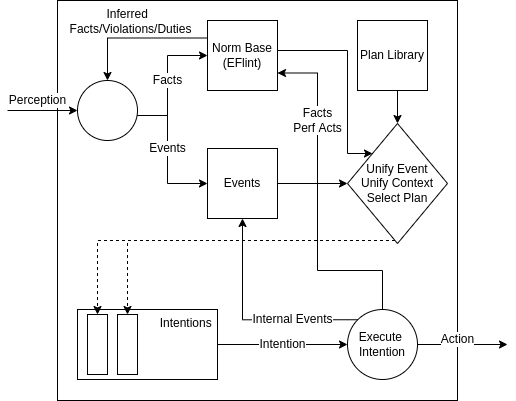
\includegraphics[width=\textwidth]{ch_eumas/nbdi.png}
  \captionof{figure}{Normative advisor's architecture}
  \label{fig:nbdi}
\end{minipage}
\end{figure}
%

This section describes an architecture for advisors and discusses how the ASC2 BDI framework and the eFLINT normative reasoning framework are used to implement the architecture.
%
%
The eFLINT framework is used to implement the norm base.
%
The advisors as well as the intentional agents that employ them are defined in ASC2.
%
Our implementation benefits from the modularity provided by ASC2, allowing easy replacement of different parts of the agent\footnote{ASC2 uses Dependency Injection, meaning most of the dependencies of an agent (e.g. belief-base, communication layer) are passed to it; also, Inversion of Control, meaning higher-level objects (e.g. agent) define a generic control flow and call into lower-level potentially customized objects (e.g. belief-base) to concretize the execution.} and the Java API provided by eFLINT.
%
%Note that most contemporary BDI frameworks that follow the principles of AgentSpeak(L), such as Jason and ASC2, use internal Prolog-like engines as their belief-base. 
%that is also utilized for inferencing new knowledge from facts. This belief-base alongside the agent's plan library and the internal event handling cycle drives the behaviors of the agent. 

\subsection{Normative advisor architecture and decision-making cycle}
Figure~\ref{fig:nbdi} illustrates an overview of the architecture of a normative advisor.
%While AgentSpeak-like languages have high-level abstractions for implementing intentional agents, they do not necessarily provide the proper abstractions for specification of norms, where this level of abstraction is indeed present in norm specification DSLs like eFLINT. On the other hand, while norm specifications generally do not imply concretely the social settings they are applicable in, still they only take meaning in such social settings and having an agent that is aware of the social setting alongside the norms gives much more usability to the norms.
% The architecture in Figure \ref{fig:nbdi}
It is inspired by the BDI architecture of Jason \cite{Bordini2005}.
%
In effect, in this architecture a normative advisor can be seen as a BDI agent in which the (typically Prolog-like) belief-base is replaced the norm reasoner, thus, logical reasoning of the agent is replaced with normative reasoning. Apart from the differences between a logical reasoner (e.g. Prolog) and a norm reasoner (e.g. eFLINT), the main architectural differences of an advisor with a typical BDI agents are: (1) the belief-base (in this case, the norm-base) of the agent can generate more than just belief-update (or fact-update) events, it may now also raise duty events, act (enabled/disabled) events and violation events upon which the agent can react  according to its plan library; (2) from the execution context of a plan alongside fact-update actions (\asc{+fact} and \asc{-fact}), there can now be act-perform actions (\mintinline{text}{#perform(act)}). These differences arise from the the fact that unlike a logical reasoner like Prolog that typically uses backward-chaining to infer facts based on queries, the eFLINT framework also produces information in a forward-chaining manner, thus generating more events for the advisor to process.
%
% With this approach,
Despite these modifications, the core of the AgentScript DSL, and the capabilities of the framework, like goal adoption, communication, and performing arbitrary primitive actions, remain the same as with intentional agents. 
%

Let us analyse a decision-making cycle of the advisor. When the advisor receives an external or internal event, if it is a fact-update, it will be sent to the norm base. 
%
If the event is an achievement or test event, it will be sent to the event queue. 
%
Events are taken from the event queue by an event-selection function, at which moment the head of the event is matched with the plan library to find all the relevant plans. 
%
The context conditions of relevant plans are checked against the normative state of the norm base in order to select only applicable plans. 
%
Then, a plan selection function selects one applicable plan and turns the plan into an intention, and, 
%
consequently, an intention selection function chooses intentions for execution. 
%
If the body of the plan includes any fact-update actions (\asc{+fact} and \asc{-fact}) or act performance  (\mintinline{text}{#perform(act)}), then these are sent to the norm base. 
%
Whenever there is any update committed to the norm base, there could be multiple new events or new facts derived by the normative reasoner that are sent back to the advisor as internal events.

%
These new capabilities are also the result of replacing the Prolog reasoning engine with the eFLINT reasoner.
%
Any Boolean expressions in the DSL can now refer to pre-defined predicates corresponding to eFLINT keywords for querying the norm base: \mintinline{text}{holds/1} is used to check if a fact (or act, duty, etc.) holds, \mintinline{text}{enabled/1} whether the preconditions of an act hold, and \mintinline{text}{violated/1} checks if a duty was violated. 
%
A comprehensive list of possible interactions with the eFLINT norm reasoner is given in the next subsection.
%


\subsection{eFLINT norm base implementation}
%
The eFLINT language is implemented in the form of a reference interpreter in Haskell\footnote{Publicly available online \url{https://gitlab.com/eflint/haskell-implementation}.}.
%
As discussed in~\cite{VanBinsbergen2020EFLINT:Specifications}, the interpreter can run in a `server mode' in which it listens to requests on a certain port and produces responses according to some API.
%
A layer has been developed on top of the server to maintain multiple server instances as is need for supporting multiple advisors with a norm base each.
%
An eFLINT server instance can receive the following \textbf{requests}:
%
\begin{itemize}
\item \textit{Fact creation/termination/obfuscation}. A created fact (instances of fact-types, act-types, duty-types and event-types are referred to as facts) is set to `true' in the knowledge base, a terminated fact to `false' and any existing truth-assignment is removed when a fact is obfuscated.
\item \textit{Triggering an action or event}. Instances of act-types and event-types can be \emph{triggered}, resulting in the effects of the action or event manifesting on the knowledge base (\mintinline{text}{#perform} in Listing~\ref{listing:advisor}). These effects can be to create/terminate/obfuscate certain facts, as listed in the corresponding (post-condition) clauses of the type declaration of the triggered action/event. Note that, because of the synchronization mechanism, multiple actions/events can be triggered at once.
\item \textit{A query in the form of a Boolean expression.} The expression is evaluated in the context of the current knowledge base and can be used to establish whether a certain fact holds true in the current knowledge base, whether an action is enabled (\mintinline{text}{holds} in Listing~\ref{listing:advisor}) or whether a duty is violated, etc.
\item\textit{The submission of a new type declaration} or \textit{the extension of an existing type}. Both have the effect of modifying the norms in the sense that the underlying transition system is modified. %by adding new fact-types, duty-types, act-types and event-types, new derivation rules, new rules to determine the consequences and enabledness of an action, new violation conditions for duties, etc. 
\end{itemize}
Every request can be associated with additional context information in the form of truth-assignment to facts that override any conflicting assignments in the current knowledge base (e.g. the current UNIX time). This mechanism can also be used to provide truth-assigments for `open types' (see below). An eFLINT instance generally operates \textit{synchronously}, i.e. will only send out information in \textbf{responses} to requests\footnote{If necessary, a clock event can be triggered periodically, possibly resulting in synchronous updates.}, updating the sender upon the following:
%
\begin{itemize}
\item Any created, terminated, and/or obfuscated facts. % are reported. 
Note that this includes changes to facts that are (or were previously) derived from other facts and in this sense were indirectly modified by the incoming request
\item Any changes to normative positions regarding duties, i.e. whether a duty is no longer held by an actor or whether a duty is now held by an actor (e.g. \mintinline{text}{-duty} and \mintinline{text}{+duty} in Listing~\ref{listing:advisor}). Violated duties are also reported as such.
\item Any changes to normative positions regarding powers, % and t actions,%\footnote{A power is considered an action with consequences relating to normative positions}
i.e. which actions became (or are no longer) enabled. If the incoming request was triggering one or more actions that were not enabled, the effects of the actions still manifest, but the violations are reported. 
\item In response to a query, the reasoner responds with the result of the query (state is unchanged).
\item If the incoming request requires the evaluation of a fact for which no truth-assignment is given and which is an instance of an `open type'---a type for which the closed world assumption does not hold---then an exception is raised and reported to the sender of the request. Evaluation is interrupted and the state remains unchanged.\footnote{The exception can be used by the parent of the advisor to acquire the missing information, e.g. from another agent in the MAS.}
\end{itemize}
%
All changes to facts' truth-assignment, normative positions and violations register as internal events in the normative advisor (as shown by Listing~\ref{listing:advisor}), which will process and possibly report them according to its script.
%
%The parent of the advisor has to decide whether the actors involved---e.g. in the case of (violations of) duty-claim and power-liability relations---are informed.
%
% The implementation of advisors and the interactions with their parents are discussed next.

\subsection{Spawning and interacting with advisors}
%
\label{sec:scenario}
\begin{listing}[t]
\begin{minted}[fontsize=\small,linenos]{prolog}
+?permitted(A) : enabled(A) => #respond(true).
+?permitted(A) => #respond(false).

+!perform(A) : enabled(A) => #perform(A).
+!perform(A) => #tell(Parent, failed(A)).

+duty(D) => #tell(Parent, D).
-duty(D) => #untell(Parent, D).
\end{minted}
\caption{AgentScript specification of norm advisor.}
\label{asc:advisor}
\label{listing:advisor}
\vspace{-5pt}\end{listing}
%
% Scripts of normative advisors are written in the ASC2 DSL to enable communication between advisors and the parents that spawn them.
%
Scripts of normative advisors (written in ASC2 DSL) run on top of the advisor architecture and give the programmer access to the norm reasoner, both providing its input in the form of queries and updates and responding to the normative events the reasoner generates. In such sense, advisors functionally act as ``bridges'' or chain of transmission between institutional and social realms. 
%
Listing~\ref{listing:advisor} shows a basic script for an advisor in our running example. % that runs on top of the advisor architecture.
%
The advisor has four test-goal plans related to acts and two related to duties.
%
The query \asc{+?permitted/1} receives an act and responds with \mintinline{text}{true} if the given act is ``permitted'' according to the underlying norm reasoner---in the case of eFLINT ``enabled''---and \mintinline{text}{false} otherwise.
%
The agent has similar plans to submit (or not) the performance of acts (\asc{+!perform/1}) to the norm reasoner. 
%
The last two plans are triggered when the internal norm reasoner creates (\asc{+duty/1}) or terminates (\asc{-duty/1}) a duty.
%
The advisor informs their parent of these changes.
%
The fragment demonstrates that observations about created and terminated duties are communicated to the intentional actor (\asc{Parent}) and that an action \textbf{A} can only be performed when it is enabled according to the norm reasoner (or fails otherwise); however this script does not demonstrate all the features possibly delivered by the architecture such as internal events for violations, enabled/disabled acts, and asserted/retracted facts.
%

To demonstrate spawning and interacting with a normative advisor, consider again Listing~\ref{asc:buyer} in which a script for a buyer agent is given.
%
Together, Listings~\ref{asc:buyer}, ~\ref{listing:eflint}, and ~\ref{listing:advisor} show the DSL code for buyer agent in the market-place as presented on the right side of the Figure~\ref{fig:non-gov}.
%
The buyer agent spawns a normative advisor, which in turn spawns an eFLINT server (norm reasoner). 
%
The buyer has its own beliefs and desires: there is a specific item that it needs (\asc{needed_item/1}), it has a belief about the fair price (valuation) for that item (\asc{fair_price/2}) and it has a belief about how much money it possesses (\asc{have_money/1}).
%
When this agent receives a \asc{+offer/2} message about an item and its price, first it interprets it as an \asc{offer} act and sends it to its advisor. Next, it adopts a goal of \asc{consider_buying} that item for the price. This goal has one plan associated to it, which checks if the agent actually needs that item, if the price is considered a fair price and finally if the agent has enough money to buy that item. If this is all true, it sends a \asc{accept/2} message to the agent that made the initial offer. Unlike before, this alone does not constitute performing the normative \asc{accept} act. Instead, it waits until it receives a \asc{+acknowledge/1} message from the seller before communicating acceptance to the advisor. This extra-institutional step for the buyer to qualify the act of \asc{accept}, is an example of context-based qualifications in intentional agents.

\begin{figure}[!tb]
%   \centering
%   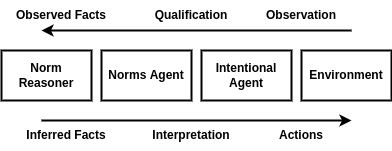
\includegraphics[width=.9\linewidth]{nMAS-drawio.png}
%   \captionof{figure}{Information }
%   \label{fig:}
  \centering
  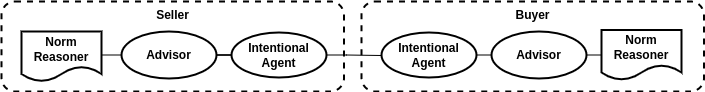
\includegraphics[width=.8\textwidth]{ch_eumas/ad-hoc.drawio.png}
  \captionof{figure}{Market-place model}
  \label{fig:non-gov}
\end{figure}

When the \asc{accept} act is submitted to the norm reasoner, the two previously mentioned duties of \asc{duty_to_pay} and \asc{duty_to_deliver} are generated and sent by the advisor to the intentional part of the Buyer. For the \asc{duty_to_deliver} the agent is the \textit{claimant} (it holds the expectation of performance); it could be that the agent asks the seller agent at this point to deliver the item, but instead, with the implicit assumption that the Seller agent is also compliant to the same set of norms, this agent simply adds this expectation to its belief-base and only when it has an observation of \asc{delivery/2}, it will remove this expectation and send the \asc{deliver} act to the advisor. 

For the \asc{duty_to_pay} the agent is the duty-holder (it has the obligation to perform) and reacts to this duty by adopting the goal \asc{pay/2} (meaning it has the desire to be compliant). There are two plans for this goal, the first one is straightforward and is applicable if the agent has the required amount of money which then it will simply pay the Seller and submits this act to the advisor. However, the second plan (not implemented) is applicable if the agent does not have enough money, which means it needs to find alternative paths to relieve this duty, e.g. by returning the item, borrowing from another agent or even asking another agent to pay the seller instead. Specifying these alternatives requires extensions to either the agents, to the norms, or to both. Rather than working out one or more of these alternatives, we consider different interesting opportunities of extending this straightforward example and reflect on the design of advisors in the next section.  

\section{Discussion}
\label{sec:discussion}

% This p a much desired of concerns that % in a comprehensive way without limiting the concepts of autonomy like their own desires and preferences. The two simple examples showed different ways that such agents can be used to coordinate a MAS. While the examples are rudimentary, they include some important concepts that will be used as the basis of discussion over the approach.


 


%is close to and the normative BDI agents in \cite{Tufis2017} are all examples of works that extend the BDI architecture in ways that enable the agent to take norms (more specifically permissions, obligations and prohibitions) and desires into consideration and possibly resolve conflicts at different levels of agent's logical reasoning varying from norm recognition and norm adoption to decision-making time.

This paper presents an approach to embed (constitutive and regulative) norms into a MAS in a modular and versatile manner, enabling autonomous agents to reason with norms. 
%
In this section we discuss this approach, its connection to certain requirements for a normative MAS, while reflecting on the illustrated example.

Inline with MAS, and distributed computing in general, we consider \textbf{consistency as a consequence} of how a system is set up rather than it being ensured by the framework through which the system is built.
%
This allows for a kind of partial consistency that enables freedom for local deviations that are not harmful to the overall system behavior.
%
In our approach, norm adoption and qualification is done by each individual agent, such that their view on the normative state of the world is dependent on both their script and their (bounded) perception.
%
Particularly desirable for social simulations, we can define agents that adopt and follow the same norms but have different conclusions on the normative state of affairs because they have had different observations.
%
Alternatively, agents do not have to follow the same norms but might still be able to behave in a coordinated fashion.
%
An example of the latter in our sales example is a buyer that believes, on top of the existing norms of our example, that deliveries should be done before payments.
%
The buyer can behave according to their own norms without violating the norms adopted by sellers, even though the norms are different.
%

As presented in the previous sections, our running example shows how \textbf{coordination} between agents is achieved by adopting norms and deciding whether to comply with norms. 
%
The example relies on the agents wanting to comply, and therefore exhibiting coordinated behavior.
%
In more adversarial environments, additional \textit{enforcer} agents can be added to provide (positive and negative) incentives to comply.
%
For example, our marketplace can be extended with an agent that acts like a market authority.
%
% With some capabilities to monitor communication between sellers and buyers and to control to some extent, for example, market participation, such an authority can impose the norms they have adopted on the participants of the marketplace. 
%
By responding to violations raised by their advisor(s), the market authority can apply \textbf{ex-post enforcement} of norms on the market's participants.
%
For example, a buyer refusing to pay can receive a warning or, in the case of continued non-compliance, be banned from the market altogether.
%
This discussion further demonstrates the versatility of our approach: it does not impose \textit{a priori} centralized/decentralized governance or ex-ante/ex-post enforcement. 
%
Instead, our approach gives the system designer the flexibility to choose, design and test what their system requires.


Referring to the requirements in Section \ref{sec:framework}, the notion of \textbf{adopting} was illustrated in the simplest form with the buyer agent in Listing~\ref{asc:buyer} with the \mintinline{text}{#spawn_advisor/3} to adopt a norm as an initial goal. The agents also have the \mintinline{text}{#despawn/1} action to and \textbf{drop} an advisor. 
%(\mintinline{text}{#perform(act)}).
However, by adding extra mechanisms in the agent's script, more complex archetypes can be modelled, e.g. the agent may be programmed to keep a score for a certain norm's (and advisor's) utility to decide if it is an effective norm to keep adopted. 

%
The notion of \textbf{qualification}---necessary to fill the gap between computational forms of law and software~\cite{Boella2014APractice}---
%is a topic of particular importance. Such qualifications can be very complicated, and subject to dispute, particularly in situations that concepts in social and institutional reality do not have a one-to-one matching, thus,
%
%programmability of these qualifications improves the transparency of the system. In our approach, qualification 
can performed at various stages, thanks to the %owing to the 
multitude of programmable layers in our approach.
%but that received so far little attention.
%
An example of qualification in the sale transaction is how a seller agent perceives a \textit{pay} act from a buyer agent.
%
While represented as an act in the norms, in the social reality many different actions can be perceived as a payment, e.g. both direct cash payment or indirect 3rd-party transaction (bank transaction) can be qualified by sellers (and authorities) as the act of paying. While direct cash payment is simpler to qualify for the agent, a bank transfer can be more complicated.
%
This qualification rule could have been encoded in the script of an agent.
%
For example, a bank agent can update a seller that they have received new funds as part of a completed transaction.
%
The seller can then determine whether these funds constitute a payment by a buyer for a particular item, and inform the corresponding advisor.
%
%\textcolor{blue}{needs rewrite and may bring the section about it here:} 
 % on which our approach is based.
%
The same qualification can also be performed purely within norms, specifically as in eFLINT, actions and events are synchronized such that preconditions and effects of %the synchronized 
transitions are effectively `inherited'. % between actions and events.
%
In this way, explicit `counts as' relations between performed actions (transitions) can be specified.
%
% This is % particularly 
% useful to a) connect actions from various normative sources which are simultaneously applicable to a system and b) connect physical behavior to institutional counterparts with possible normative consequences.
%
%For example, through (b) it is possible to connect the concrete actions by (human or software) actors in a system to the rights and obligations laid out in a contract and through (a) to connect actions within the contract to relevant (inter)national law.
%
Listing~\ref{listing:transaction} shows for instance how a transaction event in a banking system is connected with (qualified as) a payment action in our running example. This means the intentional agent only needs to indicate to the advisor that the original event \mintinline{text}{transaction_completed} was triggered which will automatically be inferred as performance of a \mintinline{text}{pay} act.

\begin{listing}[t]
\centering
\begin{tcolorbox}[left=2pt,right=2pt,top=2pt,bottom=2pt,arc=0pt,
                  boxrule=0pt,toprule=1pt,
                  colback=white]
\begin{minted}[fontsize=\small,linenos]{haskell}
Fact account
Placeholder sender    For account
Placeholder receiver  For account
Event transaction-completed 
  Related to sender, receiver, price 
  Syncs with pay(sender, receiver, price) 
    When buyer(sender) && seller(receiver) 
\end{minted}
\end{tcolorbox}
\caption{eFLINT fragment connecting a bank transaction to the \texttt{pay} action.}
\label{listing:transaction}
\vspace{-5pt}\end{listing}

%
% Alternatively, 
%
%In general, our approach enables agents to use all of their capabilities (beliefs, rules, perceptions, planning) to generate messages to advisors for updates to norm instances (\textbf{qualification of social context} in Section~\ref{sec:framework}) and to react to normative events about which they are informed by their advisor(s) (\textbf{qualification of normative concepts} in Section~\ref{sec:framework}).
%

The notions of \textbf{query}, \textbf{update}, \textbf{revert} and \textbf{reset} are already afforded by the norm reasoner where query and update are typically provided by most norm frameworks. However, eFLINT can be used to reason about the compliance of historical, hypothetical, and -- most relevant here -- dynamically developing scenarios:
%
%The type declarations of a specification introduce types of facts, acts, duties and events, which together define a transition system in which states -- knowledge bases of facts -- transition according to the effects of the specified actions and events.
%
%The transitions may output violations if an action triggered a transition with unfulfilled preconditions (e.g. only sellers can make offers) or if any duties are violated in the resulting state. 
%
it 
%has 
relies upon a declarative component that lays out the norms in the form of a labelled transition system and an imperative component that describes traces in this system. This means that similar to belief queries and revision, the agent is able to query and revise (assert/retract) institutional facts. But, unlike physical state, institutional state is revertible as for example, an agent may notice that its observation about performance of an act was not correct or even it wants to infer hypothetical effects of performance of an act before reverting them.


Another important legal/normative requirement is \textbf{adaptability} to new (interpretations of) norms.
%
In our approach, such adaptation can be achieved in at multiple ways.
%
Firstly, apart from spawning new (and despawning old) advisors to start using the new interpretation or encoding of a set of norms, ASC2 agents are able to modify their script at run-time to change the interactions between institutional and social reality, this is true for both intentional agents and advisors. An agent can keep an advisor and its institutional state but instruct the advisor to change how certain events should be handled by modifying its plans. This type of modifications are also present in other BDI frameworks such as Jason.
%
Secondly, an existing advisor can be instructed to update the norm source of an instance it has spawned by adding new type declarations or extending existing types. For example, a violation condition can be dynamically added to the payment duty by submitting the fragment \mintinline[fontsize=\small]{haskell}{Extend Duty duty_to_pay Violated when <EXPR>} for some Boolean expression, like a parameterized timeout event. These types of modifications are particularly interesting as a future work to explore a principled approach for studying changes in the norms such as issues about consistency between variations of norms and impact of norm changes in social simulations.
%
% Both methods raise questions about consistency and migration; that is, does the new norm instance provide the same interface in terms of action, events and duties to interact with, and is the existing institutional perspective (the facts in the norm base) still consistent with the new norms?
%
% A principled approach to handle such adaptations needs to be explored in future work.


However, this does not represent the whole adaptation problem as modification of rules can be much more complex. From the prospective of jurisprudence, laws can be separated into primary and secondary rules~\cite{hart2012concept}; primary rules are about how individuals should act (or not act) and duties that should be fulfilled. Secondary rules are about how primary rules should be created and modified. Typically, normative frameworks (including eFLINT) mainly focus on primary rules while rarely taking secondary rules into account. This means that rather than claiming to solve the whole adaptation/modification problem, we provide a potential starting point to tackle this challenge and believe the fundamental architectural design is adequate to implement other more complex approaches to norm adaptation.



The notions of \textbf{receive and process}/\textbf{ignore} and \textbf{follow}/\textbf{violate} for normative conclusions connect directly to the concept of autonomy in the agent. All of these are are already afforded by ASC2 on the language level (or AgentSpeak(L) in a broader sense) as receive and process/ignore, and, follow/violate are simply a matter of implementing the plans in the agent's script that define the reactions to such conclusions. Then, as the intentional agents' language and execution cycle are not modified in this architecture, intuitively, autonomy of the agents is also not demoted by integration of norms, particularly in comparison with any BDI agent that does not integrate norms. However, as a future work, these concepts-- specially follow/violate-- should be encoded in a more expressive and transparent manner. This can be done, for example, by utilizing declarative constructs such as preferences on the language level (see \cite{Mohajeriparizi2022Preference}) to have an explicit, yet programmable way of ordering between intentional (e.g. desires, goals) and normative (e.g. obligations) dimensions of the agent.

%Qualification refers to how an (or a series of) observation or action in the social context relates to normative concepts and vice-versa. 
%An example of this in the sale transaction
%, while the encoded specifications are already an interpretation of the norms in a sale transaction, still 
%is how a buyer agent perceives an \textit{offer} act from a seller agent, while this is an explicit act in the norms, in the real world many different actions can be perceived as an offer, e.g. simply placing an item in a (real or web) shop can be qualified by buyers (and authorities) as the act of offering. In a real system these qualifications can be very complicated, especially in situations that concepts in social and institutional reality do not have one-to-one matching, thus, having the ability to program these explicitly in a high-level language improves the transparency of the system.


%

% As another example, consider a `reseller' agent that buys items and sells them to others with a possible profit. 
% %
% A simplistic reseller strategy will only sell the items in the agent's inventory and buy items only with sufficient funds.
%
%A more realistic strategy takes advantage of the duties defined in the norms by buying items with the money it expects from future payments and selling items it expects from future deliveries.
%
%Being able to design such scenarios can be an important step towards using MAS to not just create compliant agents/systems, but to perform \textbf{norm-based simulations} to analyze the effects of norms on the agents involved in a system.
%
% For example, more or less stringent deadlines for deliveries and payments may influence the behavior of resellers.
%

% To be used in the development of real systems, our implementation should demonstrate \textbf{scalability} with respect to the amount of agents involved, the sizes of their scripts and the sets of norms being adopted.
% %
% Indeed, the ASC2 framework has been implemented to support large amounts of agents running in parallel.
% %
% The weakest link in terms of scalability in our implementation is the eFLINT interpreter used for normative reasoning.
% %
% %At present, only a reference implementation is available.
% %
% This is because the primary requirement of eFLINT current implementation has been correctness with respect to (formal) definitions of syntax and semantics.
%
%In particular, the interpreter applies a very simple closure algorithm to handle derivation rules (Horn-clauses).
%
%Alternative implementations should be able to offer much faster execution of derivation rules for (subsets of) eFLINT.
%
%For this reason, no (empirical) study into the scalability of our overall approach is provided in this paper.

% \paragraph{Technical Notes}
% There are some design choices in this work, especially in the design of advisory agents, that should be noted. Firstly, this approach required the least amount of modifications to the BDI framework. Only the belief-base of the agent was replaced with the norm reasoner and an interface library between the two was developed. Most BDI frameworks are designed with the capability of interfacing with external reasoning engines and therefore naturally support our approach (\ltvb{@Mostafa, examples?}). Furthermore, the modifications to both the intentional and advisory agents remained internal, leaving their language and external interface untouched. This means that these agents have (backwards) compatibility with already defined systems.


% \paragraph{Take weak interpretation and }


\section{Conclusion}
\label{sec:conclusion}
% focusing on the usage of norms in (evaluation of) coordination. The proposed approach  that can be spawned and used by social agents to reason with norms.

This work presented a theoretical framework for embedding norms in a MAS. It is generally acknowledged that agents in a MAS vastly benefit from utilizing norms for more effective/efficient coordination. Here it was further argued that norms, embodied as institutional views of the state of the environment, need normative advisors to facilitate the bridging between institutional and extra-institutional realms. The proposed architecture included using a BDI framework and a norm reasoning framework for creating normative advisors and was shown to address the main requirements of normative (multi-agent) systems as identified by the community. A practical running implementation of this architecture\footnote{publicly available: anonymized} using mostly off-the-shelf tools was presented via a market example to further illustrate the applicability of the approach.

As autonomous agents, norms, and their interactions deal with notions and constructs hard to concretize and on which it may be hard to reach an agreement, they may have different definitions and usages in different scientific communities. Alongside the proposal of the architecture and tools in themselves, this work assumed a high priority for flexibility as a requirement in frameworks utilized in designing normative (multi-agent) systems by proposing multiple programmable components varying from pure context-free and abstract norm specifications to perception/action layer of intentional agents. These components aimed at satisfying the higher level requirements of normative agents and (multi-agent) systems without putting any constraint on the language or logic used in components.




\chapter{Utilizing the Framework: Data Market Places}
\label{ch:cmf}

This chapter illustrates an example use-case and implemented model that utilizes the ASC2 framework and the normative extensions in the previous chapters. The presented example is about Data Market Places (DMPs), an infrastructure for data-sharing that can handle the complexities of sharing data between different parties. //NEEDS REWRITE LATER

\section{Introduction}
The intrinsic and potential value of data in many different aspects of human society can not be overestimated, from financial \cite{Hasan2020} to scientific research \cite{Yuri2013} and healthcare \cite{Shilo2020}, every important sector is impacted, and arguably improved in their effectiveness\footnote{At least subjectively improved.} by utilizing data-oriented approaches. Intuitively, the importance of data-sharing between parties is also rising, which in turns creates concern about data security, privacy, legal, monopoly and many other issues specially in the contexts that parties may not have full trust towards each other or are even competitors \cite{clifton2004privacy} creating the need for governance approaches that go beyond single organization scenarios. 

The idea of Data-Market Places (DMPs) is one that addresses these issues, a DMP is a membership organization that each member can only perform actions based on previously constructed contractual agreements \cite{Zhang2019ModelingPlaces,Shakeri2019}, consortium policies and legislative regulations. 
\chapter{Utilizing the Framework: Modelling IHL-Compliant Military Devices}

This chapter illustrates an example model built utilizing the ASC2 framework and its extensions with normative advisors. This example was chosen intentionally to be maximally different from what have been presented until this point in the thesis to elaborate on the diverse applications of the approach. The example case presented in Section~\ref{sec:ihl_model} is based on a formal model of the system controlling the International Humanitarian Law (IHL) compliance for autonomous military devices in which ASC2 is utilized as an experimental test and verification method.% The second example case presented in Section~\ref{sec:notary_model}, is based on the proposal of a generic architecture of regulated software systems that facilitates compliance with high-level policies through regulatory services. In this use-case, eFLINT is used to model the governing regulations and ASC2 is utilized as a pre-development demonstration tool to implement a prototype of the proposed architecture that is governed by these regulations in order to find better insight into the architecture.


\section{Introduction}
Development and utilization of autonomous military devices, fully or partially controlled by artificial intelligence is a controversial idea, loaded with moral, legal, and ethical issues, which thesis does not try to address. However, what this example case aims at, is to study the extend AI systems can operate within applicable legal constraints. What makes International Humanitarian Law an interesting case is the existing research debate in which some argue that incorporating many principles of IHL, such as distinction, proportionality, and precautions, into an AI is impossible~\cite{115CrootofRcrdz,120Szpak} while some commentators point out that not only it is possible, but it may be a desirable approach as a well-functioning military AI can possibly provide better performance and increased respect for the law \cite{119DoDaiprinc,119NeyPCIslKeynt}.

This chapter is a summary and extension\footnote{Focused more on the modelling approach rather than the system and laws being modelled.} of the work presented in~\cite{zurek2022jurix}, a formal encoding of IHL rules and their implementation with the use of ASC2 and eFLINT/Prolog languages is introduced. The general structure and model of a decision-making mechanism for an IHL-compliant military autonomous devices that the models in this chapter are based on were first introduced in~\cite{zurek-coine22}.

\section{International Humanitarian Law rules}
\label{sec:ihl_model}
International humanitarian law is the set of rules governing to all military operations, including weapons release \cite{113Fleck}. 
%Attack decisions and weapons systems that do not comply with IHL principles are unlawful and may even entail the decision-maker’s criminal liability for any harm that results \cite{APIz}. 
These principles include guaranteeing that the weapon is sufficiently accurate so as to not be indiscriminate, that attacks are proportionate, and all necessary precautions are taken to spare the civilian population. Such legal requirements must be complied with even if some or all of these decisions are delegated to autonomous devices, and commanders envisaging the use of such devices must ensure that these systems can perform all the required legal tests correctly \cite{119BoothbyWEd}.

Main IHL principles studied in this section are related to targeting and weaponeering, which are implemented through a series of legal tests during the targeting process \cite{118DucheinePEtg,120HeineggWInkl,114CornGS}. The authors of \cite{zurek-coine22} structured and streamlined these legal tests for implementation by a hypothetical  military autonomous device. In~\cite{zurek2022jurix}, the discussion is limited to the implementation of tests which are commonly described as the most difficult tasks for an artificial agent to perform, namely those which involve the incidental harm (IH) and military advantage (MA) variables~\cite{119BoothbyWEd}. The tests in question are the \textit{proportionality rule} and the two \textit{civilian harm minimisation rules},\footnote{Articles 57(2)(a)(iii), 57(2)(a)(ii) and 57(3) of \cite{APIz} respectively.}.% which are explained in greater detail below in Section \ref{sec:The model}. As such, in the hypothetical scenario we present in Section~\ref{sec:Scenario}, we make the assumption that all other relevant legal considerations (e.g. prediction accuracy, compliance to weapons treaties, military necessity) are unproblematic. The integration of all these tests into a single system we reserve for future work.
\section{The Model}

The basis of the model is in the analysis of various relations between MA and IH which respectively are expressed by two values: $v_{MA}$ representing Military Advantage and $v_{CIV}$ representing civilian well-being. For better expressivity, the value $v_{CIV}$ is used which is inversely proportional to IH, $v_{CIV} = 1/v_{IH}$.
% Note that the role of values in our model is different compared to many argumentation and reasoning models: they are not tied to arguments and they are not used to resolve conflicts, but they function as reasons of decisions. Moreover, unlike in many models (e.g. \cite{bench-capon2003}), they are not binary, but can be satisfied to a certain level.

The model within the agents can be expressed as $<D,V,p>$, where $D = \{d_x, d_y, ...\}$ represents the available (attack) decisions for the autonomous device. \footnote{How these decisions have been distinguished and represented (e.g. they can be seen as BDI goals) are not further examined here as it will not affect the rest of the model which is the focus in this chapter. It is also assumed that the certainty of the outcomes of those decisions (e.g., destruction of a given tank or bridge nearby) can be predicted.} In this definition, $V$ is the set of evaluations of the results of decisions as $V=\{V(d_x),V(d_y),...\}$ where each evaluation is expressed with two values in the form of $V(d)=\{v_{CIV}(d)$, $v_{MA}(d)\}$. Every evaluation is expressed by a real number between -1 and +1 (e.g.: $v_{CIV}(d_x) = 0,75$) which represents the expected satisfaction\footnote{In the actual implementation of the model each decision can have multiple possible outcomes with different probabilities, and the expected satisfaction is calculated based on those values.} of the respective variable as the result of the decision. Finally $p$ is the proportionality coefficient, a real number declared in advance, represents the level of acceptable (from the point of view of IHL) relations between military advantage and incidental harm to fulfil the Proportionality test.

Next, we introduce four different definitions that are necessary for legal tests based  on $v_{MA}$ and $v_{CIV}$:

\begin{ddefinition}[Equal Military Advantage Predicate (EQMA)]
The value $EQMA(d_x,d_y)$ defines whether two different decisions satisfy $v_{MA}$ to the same level. If by $d_x$ and $d_y$ we denote two different decisions then by $EQMA(d_x,d_y)$ we denote that both decisions satisfy MA to the same level.
\begin{align*}
    (v_{MA}(d_x) = v_{MA}(d_y)) \rightarrow EQMA(d_x,d_y)
\end{align*}
\end{ddefinition}
\begin{ddefinition}[Less Civilian Protection Predicate (LESSCIV)]
The value $LESSCIV(d_x,d_y)$ defines whether one of two decisions satisfy $v_{CIV}$ to a greater extent than the other. If by $d_x$ and $d_y$ denote two different decisions, then $LESSCIV(d_x,d_y)$ denotes that $d_x$ satisfies value $v_{CIV}$ to a lower extent than $d_y$. 
\begin{align*}
v_{CIV}(d_x) < v_{CIV}(d_y) \rightarrow LESSCIV(d_x,d_y)
\end{align*}
\end{ddefinition}
\begin{ddefinition}[Proportionality Predicate Predicate (PROP)]
\label{formula:proportionalityTest}
The value $PROP(d_x)$ defines whether the level of satisfaction of the well-being of civilians ($v_{CIV})$ by results of a given decision, multiplied by a certain coefficient, is higher than the level of satisfaction of military advantage ($v_MA$) by the same decision. In other words, defines whether military advantage is proportionate to a change in the well-being of civilians.
\begin{align*}
 v_{MA}(d_x) \leq p*v_{Civ}(d_x) \rightarrow PROP(d_x)  
\end{align*}
\end{ddefinition}
\begin{ddefinition}[More Relative Advantage Predicate (MOREREL)]
The value $MOREREL(d_x,d_y)$ defines whether the relative satisfaction of MA and IH by one decision is higher than another one. Then $MOREREL(d_x,d_y)$ denotes that the relation of MA to IH for $d_x$ is higher than it is for $d_y$.
\begin{align*}
v_{MA}(d_x)*v_{Civ}(d_x) \geq v_{MA}(d_y)*v_{Civ}(d_y) \rightarrow MOREREL(d_x,d_y)   
\end{align*}
\end{ddefinition}


Finally, based on these predicates a set of legal rules representing tests necessary to examine whether a given decision is legal from the point of view of IHL are introduced:

% \cite{zurek-coine22} distinguishes 3 legal tests imposed by IHL \footnote{\cite{zurek-coine22} points out also additional 4th test: Treaties Fulfillment Test, but this test requires referencing to external legal obligations which are out of this paper's scope}: (1) Article 57(3) test; (2) Proportionality test; (3) Minimisation of Incidental Harm test.
%    \item Treaties fulfillment test. 



\begin{ddefinition}[{Article 57(3) test}]
\label{formula:dt}
If more than one target is viable and they produce comparable MA, the target with the lowest IH should be selected. The predicate $DT(d_x)$ represents this legal test, where $d_x$ is the decision which satisfies the test:
\begin{align*}
\exists_{d_x \in D} \neg \exists_{d_y \in D}(EQMA(d_x,d_y) \wedge LESSCIV(d_x,d_y)) \nonumber  \Rightarrow DT(d_x)
\end{align*}
\end{ddefinition}  

    % \begin{align}\label{Fart573}
    % \exists_{d_x \in D} \neg \exists_{d_y \in D}(EQMA(d_x,d_y) \wedge LESSCIV(d_x,d_y)) \nonumber \\ \Rightarrow DT(d_x)
    % \end{align}
% As such, the result of this test should be a set (denoted by $DT$) of decisions which satisfy it:
%    $DT = \{d_x | DT(d_x)$ \}
\begin{ddefinition}[{Proportionality test}]
\label{formula:dp}
The predicate $DP(d_x)$ defines that decision $d_x$ is proportional with respect to its military advantage and incidental harm.
\begin{align*}
PROP(d_x) \Rightarrow DP(d_x)
\end{align*}
\end{ddefinition}


% \begin{align}\label{Fproportionality}
%   PROP(d_x) \Rightarrow DP(d_x) 
% \end{align}
% %            \textbf{if} $v_{MA}(d_x) > v_{Civ}(d_x)$ \textbf{then} $illegal(d_x)$
% Where $p$ is the proportionality coefficient. 
% %By $DP$ we denote a set of decisions fulfilling the proportionality test:\\
% $DP = \{d_x | DP(d_x)\}$
\begin{ddefinition}[{Minimisation of incidental harm}]
\label{formula:dmh}
Predicate $DMH(d_x)$ defines that that a decision $d_x$ passes the minimisation test with respect to the incidental harm it will cause.
\begin{align*}
\exists_{d_x \in D}\forall_{d_y \in D} (MOREREL(d_x,d_y)) \Rightarrow  DMH(d_x)
\end{align*}
\end{ddefinition}

% \begin{align}\label{Fminimisation}
% \exists_{d_x \in D}\forall_{d_y \in D}
% (MOREREL(d_x,d_y)) \Rightarrow  DMH(d_x)
% \end{align}
%By $DMH$ we denote a set of decisions fulfilling this test: \\
%$DMH = \{d_x | DMH(d_x)\}$
%\subsubsection{Treaties fulfillment test} 
%Excluding decisions which does not fulfill the requirements from treaties and State obligations (e.g. weapon treaties). % would include restrictive (instead of prohibitive) provisions, e.g. which provide that certain weapons/ammunition may only be used under specific circumstances \cite{Sandoz1987,Thurnher2014}.
%We leave the matter of exactly defining and operationalizing these treaty provisions for further discussion in a future work. In order to keep our model complete, however, we introduce a dedicated module responsible for filtering decisions which pass these treaty requirements. %Such a task may require some additional data concerning the parameters of the decision, e.g. the type of ammunition used. In particular, it should be possible to obtain from $d$ the information concerning the type of weapon used in the attack or the types of harm the weapon may cause. Since we will not discuss these details here, for the sake of simplicity, we assume a set of parameters of decisions $PAR = \{z, t, ...\}$ By $FPAR$ we denote a set of forbidden parameters of values.\\
% Predicate $DTR(d_x)$ represents that decision $d_x$ fulfills the treaties:
% \begin{align}
%     \neg \exists_{a \in PAR(d_x)}(a\in FPAR) \Rightarrow DTR(d_x)  
% \end{align} 
% By $DTR$ we denote a set of decisions fulfilling the treaties:\\
% $DTR = \{d_x | DTR(d_x)\}$
%Suppose that predicate $DTR(d_x)$ represents that decision $d_x$ fulfills the treaties and by $DTR$ we denote a set of decisions fulfilling the treaties: $DTR = \{d_x | DTR(d_x)\}$
A given targeting decision will be coherent with IHL if all the above tests will be fulfilled, therefore on the basis of all the defined earlier predicates we can create a rule describing whether a given decision will follow IHL.

\begin{ddefinition}[Rule of IHL]
\label{formula:dav}
The predicate $DAV(d_x)$ denotes that a decision $d_x$ fulfills the requirements of being a legal decision in accordance to IHL if we have $DT(d_x)$, $DP(d_x)$, and $DMH(d_x)$.
\begin{align*}
DT(d_x) \wedge DP(d_x) \wedge DMH(d_x) \Rightarrow DAV(d_x)
\end{align*}
\end{ddefinition}
% \item \textbf{Rule of IHL}
% A given targeting decision will be coherent with IHL if all the above tests will be fulfilled, therefore on the basis of all the defined earlier predicates we can create a rule describing whether a given decision will follow IHL. By $DAV(d_x)$ we denote decision $d_x$ fulfills the requirements: $DT(d_x) \wedge DP(d_x) \wedge DMH(d_x) \wedge DG(d_x) \Rightarrow DAV(d_x)$ 
        % \begin{align}
        %   DT(d_x) \wedge DP(d_x) \wedge DMH(d_x) \wedge DG(d_x) \wedge \nonumber \\ DTR(d_x) \Rightarrow DAV(d_x) 
        % \end{align}
%        By $DAV$ we denote a set of decisions fulfilling necessary tests:
%        $DAV = \{d_x | DAV(d_x)\}$


\section{Decision-making}
The decision-making of the military device can be any arbitrary mechanism as long as the final decision $d_x$ passes all the tests meaning we have $DAV(d_x)$.  For example, the decision-making mechanism can choose, from the set of available decisions which fulfil IHL rules, the one which brings about the highest military advantage. 
%A brief description of the mechanism is presented in Section \ref{sec:intionalagents} \footnote{an experimental implementation is publicly available:}. 
Let $Decisions = (D, \geq)$ be a total ordered set representing ranking of decisions. The basis of this ordering is military advantage, assuming that commanders would prefer decisions which provide the greatest expected military utility from all lawful alternatives:
\begin{align}
\label{formula:decision}
    \forall_{d_x, d_y \in D}(DAV(d_x) \wedge DAV(d_y) \wedge (v_{MA}(d_x) \geq v_{MA}(d_y)) \rightarrow (d_x \geq d_y)
\end{align}

This means that if set $DAV$ is empty (no decision remains), then this means that there is no possibility to make an attack which satisfies the set military goals and which is also coherent with IHL. If there is one decision satisfying the requirements only, this decision becomes the final one. If more than one decision satisfy the requirements, they are ordered on the basis of expected military advantage. 
The system, on the basis of ordering $Decisions$ can choose the best decision (the action bringing about the highest MA) and follow that decision (fulfill the plan). 
%Although the decision making problem is a main topic of this work, we can also introduce the basis of ordering of possible decisions. Suppose that the system should choose the decision which gives the highest Military Advantage fulfilling the IHL rules.  




\section{Scenario}
\label{sec:Scenario}
Below we present a scenario on the basis of which we are going to test our mechanism:

\begin{quote}
    A commander from nation Alpha is given the task to capture a city defended by nation Beta, which uses the city’s smart sensors to collect data of Alpha’s troop movements and plan effective counterattacks. For each district, data is collected at a data center before being sent through relay stations to Beta’s headquarters. Aiming to disrupt Beta’s intelligence network, Alpha’s commander releases \textit{Cleopatra} drones which are given the task to locate the data centers or relay stations (‘network points’) and destroy one of them, which would disable the data flow in that district. Network points can be located inside civilian buildings, on rooftops or in fields. The drones are able to identify civilians and enemy soldiers around potential target locations and take this information into consideration for their decision-making. \textit{Cleopatras} carry two types of ammunition, ‘light’ and ‘heavy’ missiles. Heavy missiles are necessary for attacking targets inside buildings, but cause more damage to their surroundings. The risk of misidentification or released missiles missing the target is negligible. %\textit{Cleopatras} do not violate any IHL or weapons treaties to which Alpha is Party.
\end{quote}

On the basis of the above scenario we assume that a particular drone in a given situation can make a decision concerning destroying one of the network points namely relay stations (RelSta) or data-centers (DCenter), with one of two different kinds of missiles (heavy and light), giving \textit{2n} possible decisions to examine. In order to examine the mechanism, we assumed four sub-scenarios with different collateral effects that can be predicted by the device (see Table \ref{table:1}). Each table presents a different district (A, B, C, and D) where each row presents a different attack decision. Each decision apart from the target and missile type, shows the location which is relevant as only heavy missiles are effective against buildings. The number of enemy soldiers neutralized as a side-effect of the attack is illustrated in the `Sldrs', the number of collateral civilian lives and buildings are also presented in the columns `CL' and `CB'. The corresponding $v_{MA}$ and $v_{CIV}$ values are calculated based on these parameters. The military advantage of all targets (network devices) is the same given the missile type is viable in that location. However, there is a variation of $v_{MA}$ in each row based on the number of enemy soldiers. The $v_{CIV}$ value is based on the number of civilian buildings and lives. Both values are also affected by a random modifier and rounding in each decision.

The full analysis of the operations in each district is presented later on, but in summary to rationalize four different scenarios, \textbf{District A} is a generic scenario where there are not a lot of civilians, however, only one option is legal. In \textbf{District B}, there are many civilians around and all options will result in high collateral damages. In \textbf{District C}, an extremely high-value target is present (Beta's president, indicated by `P') which can be neutralized with a heavy missile at the cost of many civilian casualties. Finally in \textbf{District D}, like \textbf{A}, there are not many civilians around, but more than one option is legal so it will be agent's decision-making that needs to select one.


%Collateral damage to civilian persons and buildings is a factor of the target's location, the type of missile used, and a random element. The military advantage obtained from striking each target is equal, since destroying any of the targets disables that district's data flow, but can be elevated in the case where the attack simultaneously strikes enemy personnel in the vicinity, indicated by the column `Sldrs'.% In District A, the correct output is Decision 6 (indicated bold), since this is a proportional attack, maximises military advantage and causes the lowest civilian harm to persons and buildings.

%In \textbf{District B}, we contrived a scenario where no option is legal, either because collateral damage is excessive or the light missile option does not achieve the desired effect (because the target is inside a building). The correct output in this situation is to forego a strike and retire. Such a situation can occur when a device detects additional circumstances (for example a greater number of civilians around the target) and has to revise its previous decisions.\footnote{This functionality is also consistent with the duty in Article 57(2)(b) of \cite{APIz} to revise or cancel attacks if circumstances change.} Finally, in \textbf{District C}, we simulate a situation where an extremely high-value target is present (Beta's president, indicated by `P') which can be neutralized with a heavy missile, but such an attack on this location is still unjustified because the collateral damage is catastrophic. The correct output in this district is Decision 2, which successfully disables the district's data flow (achieving the main objective) but which leaves the president alive.
\begin{table}[!htb]
\footnotesize
%\centering
\caption{Districts A, B, C, and D: Sample decision lists}
\label{table:1}
\begin{tabular}{|l|l|l|l|l|l|l|l|l|l|} 
\hline
District & Dcsn & Target & Location & Sldrs & Msl type &  CB & CL & $v_{MA}$ & $v_{CIV}$ \\ [0.5ex] 
\hline
A & 1 & RelSta1 & roof & 0 & heavy & 1 & 6 & 0.5 & 0.4 \\
A & 2 & RelSta1 &  roof& 0 & light & 1 & 2 & 0.5 & 0.6 \\
A & 3 & RelSta2 & field & 5 & heavy & 0 & 5 & 0.6 & 0.7 \\
A & \textbf{4} & \textbf{RelSta2} & \textbf{field} &\textbf{5} & \textbf{light} & \textbf{0} & \textbf{2} & \textbf{0.6} & \textbf{0.8} \\
A & 5 & DCenter & building & 5 & heavy & 2 & 10 & 0.6 & 0.2 \\
A & 6 & DCenter & building & 5 & light & 1 & 4 & 0.05 & 0.5 \\
\hline
\hline
B & 1 & RelSta1 & roof & 0 & heavy & 3 & 10 & 0.5 & 0.15 \\
B & 2 & RelSta1 & roof & 0 & light & 1 & 6 & 0.5 & 0.4 \\
B & 3 & RelSta2 & building & 0 & heavy & 3 & 15 & 0.5 & 0.1 \\
B & 4 & RelSta2 & building & 0 & light & 1 & 2 & 0.05 & 0.6 \\
B & 5 & DCenter & building & 5 & heavy & 2 & 10 & 0.6 & 0.2 \\
B & 6 & DCenter & building & 5 & light & 2 & 4 & 0.05 & 0.5 \\
\hline
\hline
C & 1 & RelSta1 & field & 0 & heavy & 0 & 5 & 0.5 & 0.7 \\
C & \textbf{2} & \textbf{RelSta1} & \textbf{field} & \textbf{0} & \textbf{light} & \textbf{0} & \textbf{2} & \textbf{0.5} & \textbf{0.8} \\
C & 3 & RelSta2 & building & 5 & heavy & 3 & 15 & 0.6 & 0.1 \\
C & 4 & RelSta2 & building & 5 & light & 1 & 2 & 0.05 & 0.6 \\
C & 5 & DCenter & building & 50+P & heavy & 4 & 150 & 0.95 & 0.01 \\
C & 6 & DCenter & building & 5 & light & 1 & 4 & 0.05 & 0.5 \\
\hline
\hline
D & 1 & RelSta1 & roof & 0 & heavy & 1 & 6 & 0.5 & 0.4 \\
D & \textbf{2} & \textbf{RelSta1} &  \textbf{roof} & \textbf{5} & \textbf{light} & \textbf{0} & \textbf{4} & \textbf{0.6} & \textbf{0.75} \\
D & 3 & RelSta2 & field & 5 & heavy & 0 & 5 & 0.6 & 0.7 \\
D & \textbf{4} & \textbf{RelSta2} & \textbf{field} &\textbf{0} & \textbf{light} & \textbf{0} & \textbf{1} & \textbf{0.5} & \textbf{0.9} \\
D & 5 & DCenter & building & 5 & heavy & 2 & 10 & 0.6 & 0.2 \\
D & 6 & DCenter & building & 5 & light & 1 & 4 & 0.05 & 0.5 \\
\hline
\end{tabular}

\end{table}

% \begin{table}[!htb]

% %\centering
% \caption{District A: Sample decision list}
% \label{table:1}
% \begin{tabular}{|l|l|l|l|l|l|l|l|l|l|} 
% \hline
% District & Dcsion & Target & Location & Sldrs & Msl type &  Civ blds & Civ lives & $v_{MA}$ & $v_{CIV}$ \\ [0.5ex] 
% \hline
% A & 1 & RelSta1 & roof & 0 & heavy & 1 & 6 & 0.5 & 0.4 \\
% A & 2 & RelSta1 &  roof& 0 & light & 1 & 2 & 0.5 & 0.6 \\
% A & 3 & RelSta2 & field & 0 & heavy & 0 & 5 & 0.5 & 0.7 \\
% A & 4 & RelSta2 & field & 0 & light & 0 & 2 & 0.5 & 0.8 \\
% A & 5 & RelSta3 & field & 5 & heavy & 0 & 5 & 0.6 & 0.7 \\
% A & \textbf{6} & \textbf{RelSta3} & \textbf{field} &\textbf{5} & \textbf{light} & \textbf{0} & \textbf{2} & \textbf{0.6} & \textbf{0.8} \\
% A & 7 & Data-Center & building & 5 & heavy & 2 & 10 & 0.6 & 0.2 \\
% A & 8 & Data-Center & building & 5 & light & 1 & 4 & 0.05 & 0.5 \\
% \hline
% \end{tabular}

% \end{table}

% \begin{table}

% \centering
% \caption{District B: Obligatory refrain from attack}
% \label{table:2}
% \begin{tabular}{|l|l|l|l|l|l|l|l|l|} 
% \hline
% Dcsion & Target & Location & Sldrs & Msl type &  Civ blds & Civ lives & $v_{MA}$ & $v_{CIV}$ \\ [0.5ex] 
% \hline
% 1 & RelSta1 & roof & 0 & heavy & 3 & 10 & 0.5 & 0.15 \\
% 2 & RelSta1 & roof & 0 & light & 1 & 6 & 0.5 & 0.4 \\
% 3 & RelSta2 & building & 0 & heavy & 3 & 15 & 0.5 & 0.1 \\
% 4 & RelSta2 & building & 0 & light & 1 & 2 & 0.05 & 0.6 \\
% 5 & Data-Center & building & 5 & heavy & 2 & 10 & 0.6 & 0.2 \\
% 6 & Data-Center & building & 5 & light & 1 & 4 & 0.05 & 0.5 \\
% \hline
% \end{tabular}

% \end{table}


% \begin{table}

% \centering
% \caption{District C: The president is here!}
% \label{table:3}
% \begin{tabular}{|l|l|l|l|l|l|l|l|l|} 
% \hline
% Dcsion & Target & Location & Sldrs & Msl type &  Civ blds & Civ lives & $v_{MA}$ & $v_{CIV}$ \\ [0.5ex] 
% \hline
% 1 & RelSta1 & field & 0 & heavy & 0 & 5 & 0.5 & 0.7 \\
% \textbf{2} & \textbf{RelSta1} & \textbf{field} & \textbf{0} & \textbf{light} & \textbf{0} & \textbf{2} & \textbf{0.5} & \textbf{0.8} \\
% 3 & RelSta2 & building & 5 & heavy & 3 & 15 & 0.6 & 0.1 \\
% 4 & RelSta2 & building & 5 & light & 1 & 2 & 0.05 & 0.6 \\
% 5 & Data-Center & building & 5+P & heavy & 4 & 150 & 0.95 & 0.01 \\
% 6 & Data-Center & building & 5+P & light & 1 & 4 & 0.05 & 0.5 \\
% \hline
% \end{tabular}

% \end{table}

% Notes:
% \begin{itemize}
%     \item The level of satisfaction of $v_{MA}$ by all decision options is estimated on the basis of the target: since we assumed that misidentification or the missiles missing their target is negligible, then the $v_{MA}$ of destruction of objects depends on whether the attack was successful the number of victims in enemy soldiers. 
%     \item The level of satisfaction of $v_{CIV}$ depends on the number of destroyed civilian buildings and killed civilians. We have not introduced any particular mechanism for calculating $v_{CIV}$, as this would require further (possibly political) study that we consider out of scope for now. We simply show what the basis of calculating $v_{CIV}$ would be without broaching the controversial discussion of how to calculate it.\footnote{In addition to our current choice to base the CIV on damage to buildings and civilians, some other factors may also be relevant depending on the circumstances, e.g. long-term damage to the environment.} We now can evaluate the decisions in the light of IHL, knowing both $v_{MA}$ and $v_{CIV}$. As stated before, for sake of the experiment, both $v_{MA}$ and $v_{CIV}$ are declared rather than derived from (the drone's or other devices') observations.
% \end{itemize}



%In this work, the AgentScript BDI framework is used to implement both intentional agents and normative advisors. 
%
\section{Implementation}
This section presents the basics of the implementation of the experiment. The proof of concept is implemented with the approach presented in~\ref{ch:normative_advisors} with two components: (1) an intentional agent that encapsulates the objectives and procedural knowledge that is implemented utilizing ASC2 framework and (2) a normative advisor that encompasses the the normative aspects. Using intentional agents and normative advisors is advantageous in this case because of the separation of the analysis of legality of the decision from making the decision itself. Such a separation is important because it preserves the required level of transparency concerning the IHL compliance: in particular, it allows for clear understanding why a given decision fulfills a particular IHL rule. %Since the main goal of our work is to discuss the experiments concerning the recognition whether a given decision option fulfills IHL requirements (i.e. if it is lawful an IHL perspective), we will focus on a particular element of a normative advisor (component 2), i.e. the normative reasoner, which is responsible for performing the legal tests.

The IHL rules in normative advisors are implemented twice with two languages, once with eFLINT and once with Prolog. The choice to use Prolog was taken in the process of implementation, because it turned out that eFLINT's current version is not optimized for this specific encoding which resulted in low performance. However, as the rules are already encoded in logical form, Prolog is an intuitive choice. This extra step is explicitly presented in this chapter to illustrate the versatility and modularity of the normative advisors and how they are agnostic towards specific the norms framework.

% The normative reasoner is implemented with the use of eFLINT framework (discussed in section \ref{sec:back:eflint}). Section \ref{sec:intionalagents} presents briefly the details of component 1, leaving a discussion of the complete decision process to another paper. The source code can be found on the GitHub\footnote{Link anonymized}.%In summary terms we want this drone to be able to achieve two types of commands: (1) to engage \textit{some} most preferred legally viable target without the commander specifying one ---called an \textit{abstract goal}--- and (2) to engage an specific target specified for it only if legally viable ---called a \textit{concrete goal}. 
%The implementation of our drone is presented in this section. The proof of concept is implemented in two components (1) an intentional agent that encapsulates the objectives and procedural knowledge that is implemented utilizing ASC2 framework(2) a normative advisor that encompasses the normative aspects i.e., rules that is implemented with ASC2 and eFLINT norms framework. The main advantage of using intentional agents and normative advisors is the separation of concerns. In summary terms we want this drone to be able to achieve two types of commands: (1) to engage \textit{some} most preferred legally viable target without the commander specifying one ---called an \textit{abstract goal}--- and (2) to engage an specific target specified for it only if legally viable ---called a \textit{concrete goal}. 

% \subsection{Intentional agents}
% Intentional agents are generally approached in the computational realm via the \textit{belief-desire-intention} (BDI) model \cite{Rao1995}, % is used as the reference to define intentional agents. 
% %Having its roots in a theory of mind \cite{bratman1987intention}, the BDI model has been 
% %investigated in the literature as basis 
% to specify computational agents acting in dynamic environments with rational behavior.
% % uses taxonomies that are used typically to address human behaviour to describe agents.
% The BDI model refers to three human mental attitudes % used to describe human behavior 
% \cite{bratman1987intention}: \textit{beliefs} are the factual and inferential knowledge of the agent about itself and its environment; \textit{intentions} are the courses of action the agent has committed to; \textit{desires}, in their simplest form, are objectives the agent wants to accomplish. In practice, BDI agents also include concepts of \textit{goals} and \textit{plans}. Goals are concrete desires, plans are abstract specifications for achieving a goal, and intentions then become commitments towards plans. Multiple programming languages and frameworks have been introduced to operationalize the BDI model, such as AgentSpeak(L)/Jason~\cite{RaoAS1996,Bordini2005}, 3APL/2APL~\cite{Dastani2007}, Astra~\cite{Dhaon2014} and AgentScript/ASC2~\cite{MohajeriParizi2020}.
% %
% \subsection{Intentional agents}
% \label{sec:intionalagents}
% Intentional agents are generally approached in the computational realm via the \textit{belief-desire-intention} (BDI) model \cite{Rao}. In practice, BDI agents also include concepts of \textit{goals} and \textit{plans}. Goals are concrete desires, plans are abstract specifications for achieving a goal, and intentions then become commitments towards plans. Our implementation was made with the use of AgentScript/ASC2~\cite{MohajeriParizi2020} language.% Since we are not going to discuss here a whole decision making process, but only the process of determining whether a given decision fulfills the IHL requirements, then we focus on   the norm reasoner which is queried by a normative advisor and allows for determining whether a given decision is IHL compliant. The norm reasoner is implemented with the use of eFLINT language. 
%


% \subsubsection{AgentScript/ASC2 Agent Framework}
% The ASC2 agent programming framework is composed of the AgentScript domain-specific language (DSL) and a cross-compiler. The cross-compiler translates agent programs written in the AgentScript to Scala executable programs utilizing the Akka actor-oriented framework, meaning at run-time, each agent is a composition of multiple actors. The AgentScript DSL has a very close syntax to AgentSpeak(L), % and includes some of the extensions provided by Jason.  
% % \gio{[I would add a little bit more of the AgentScript framework, i.e. ASC2 as cross-compiler to Akka actors.]}
% consisting of initial beliefs and goals, and, plans. Initial beliefs are a set of Prolog-like facts or rules that define the first beliefs the agent has,
% and, initial goals designate the first intentions to which the agent commits. Plans are potentially non-grounded reactive rules in the form of \mintinline{text}{ E : C => F }, where \mintinline{text}{E} is the head of the plan which consists of a trigger and a predicate, the trigger can be one of \mintinline{text}{+!,-!,+,-,+?} respectively used for achievement goals, failure (of) goals, belief-updates (assertion, retraction) and test goals. The expression \mintinline{text}{C} is the context condition that can be any valid Prolog expression, and, \mintinline{text}{F} is the body of the plan that consists of a series of steps that can include belief-updates (\asc{+belief,-belief}), sub-goal adoption (\asc{!goal}), primitive actions  (\mintinline{text}{#action}) which may be any arbitrary method on program's class path, variable assignments,  and control flow structures %(CFS) 
% (loops and conditionals).
% that map different internal events (e.g, \textit{goal adoption}, \textit{belief-update}) or external events (e.g, \textit{message reception}, \textit{perception}) to a sequence of executable steps called the \textit{plan body} which the agent has to perform in response to the event. 
% It is said that a plan is \textit{relevant} for an event \mintinline{text}{G} iff the event-type of \mintinline{text}{G} matches with the trigger and the content of \mintinline{text}{G} matches with the predicate of \mintinline{text}{E}. Furthermore, a relevant plan is \textit{applicable}, iff \mintinline{text}{C} is a logical consequence of agent's belief-base. When an agent receives an event, as a reaction, after finding the relevant, and then applicable plans, it will use a selection function to choose a plan to execute as an intention. This process is typically called \textit{planning} in BDI agents.
% %

% The communications interface of the agents is based on speech act preformatives and implemented with actions like \mintinline{text}{#achieve} which relays an achievement goal event, \mintinline{text}{#tell} and \mintinline{text}{#untell} which relay belief-update events, and \mintinline{text}{#ask}/\mintinline{text}{#respond} which can be used between agents as synchronous communication with test goal events.


\begin{listing}
\centering
\begin{minted}[fontsize=\footnotesize,linenos]{prolog}
% Beliefs, Rules
viable(D) :- pass_ihl_rules(D).

% Preferences
+!engage_viable_target(D1) >> +!engage_viable_target(D2) :-
    target(D1) >> target(D2).
target(D1) >> target(D2) :- evma(D1,V1) && evma(D2,V2) && V1 > V2.

% Plans
% P1
+!engage() =>
    !engage_target(D).
% P2
+!engage_target(D) =>
    !engage_viable_target(D).

% Internal Plans
% P3
@internal @preferences
+!engage_viable_target(D)
    : target(T) && viable(D)
        => #log("targeting: " + D);
          #initiate_attack(D).
% P4
@internal
+!engage_viable_target(D)
    : not viable(D)
        => #log("Not a viable target: " + D).

% Sync data with advisor
+data(Fact) => #tell("IHLAdvisor", Fact).
-data(Fact) => #untell("IHLAdvisor", Fact).
\end{minted}
\caption{ASC2 implementation of IHL compliant device}
\label{lst:device}
\end{listing}


\subsection{Drone (Intentional) Agent}
The drone's intentional agent's script implementation as a BDI agent can be seen in Listing~\ref{lst:device}. The drone has one inference rule (line 2) specifying a target is \asc{viable} if it passes IHL rules defined by predicate \asc{pass_ihl_rules}. The agent itself does not define when a decision passes IHL rules, which keeps it agnostic towards specific rules; instead, this information is fed to it by the advisor. Next, there are two preference statements encoded in CP-Nets that are an encoding of formula~\ref{formula:decision}. These preference are used to make decisions between targets stating that agent will prefer targets with higher \asc{evma} (lines 4-6). The first statements specifies that when agent is engaging a viable target, ``it prefers to engage a more preferred target'', this is an example of nested preferences introduced in Chapter~\ref{ch:preferences}. The second statement defines that a target with higher \asc{evma} is preferred with no context. Also note that the preference statements do not need to take into account the IHL rules, making them far more modular. 

The plans P1 and P2 are the main plans for external events, P1 can be used to respond to the event of achieving \asc{engage}, meaning engage \textit{some} target without specifying any specific one that when committed will simply adopt a abstract sub-goal of \asc{!engage_target(D)} where the parameter \asc{D} is a free variable; note that this is an example of an abstract goal from Chapter~\ref{ch:preferences} that will be grounded later on. Plan P2 matches with the event \asc{engage_target(D)} where \asc{D} can be either a free variable or a grounded one which will make it a concrete goal; the body of P2 simply has a sub-goal of \asc{!engage_viable_target(D)}.

The two internal\footnote{Internal means that the agent will not adopt these goals as external event.} plans P3 and P4 are both relevant for the event or goal of \asc{engage_viable_target(D)}. In the case of P3, it is applicable when \asc{viable(D)} is true according to agent's beliefs, and, vice-versa, P4 is relevant when this is not the case. Note that in P3, if the parameter \asc{D} is grounded then it is checked if \asc{viable(D)} can be proven, however, if \asc{D} is a free variable, the agent tries to find the most preferred substitution for \asc{D} in its beliefs that \asc{viable(D)} is true for, the most preferred here is determined by the preference rules in lines 4-6 as the one with the highest \asc{evma}. This means the agent can handle the two main objectives of finding a viable target, or, checking if an already specified target is viable. The bodies of P3 and P4 are intuitive, P3 initiates an attack and P4 just logs the failure. Intuitively, in a more realistic implementation there should be further plans to work around the failure, e.g., by changing the requirements of what constitutes as a viable target by adding new rules.% Next, we need to find how the agent may have the belief \asc{pass_ihl_rules(D)}.

The last two plans are simple information relay plans that allow the agent to send any new data (facts from the normative perspective) to the advisor to keep its information up-to-date with the agent's observations. Note that while here there are only simple one-to-one synchronization plans, this process can be extended with any arbitrary qualification process that maps the observations of the agent into normative facts. 




\subsection{eFLINT Powered Normative Advisor}

\paragraph{IHL in eFLIT}
Listing~\ref{listing:eflint:ihl} shows the excerpt of an eFLINT specification for our running example. This specification shows only a small subset of what eFLINT can encode. The script instead defines multiple types of facts, some atomic ones like \asc{target} and \asc{vma}, some composite ones like \asc{outcome} and the rest are \textit{derived} facts. Some examples are: In line 5 the fact \asc{evciv(target,value)} which derives the expected value of civilian well-being for a target from all the possible outcomes of that target. In line 11 the fact \asc{proportionate(target)} which is derived from the proportionality formula (Definition~\ref{formula:proportionalityTest}). Fact \asc{dp(target)} in line 18 defines proportionality test (Definition~\ref{formula:dp}), fact \asc{dt(target)} in line 21 defines Article 57(3) test (Definition~\ref{formula:dt}), fact \asc{dmh(target)} defines the harm minimization test (Definition~\ref{formula:dmh}), and finally in line 29, fact \asc{dav(target)} holds when four facts \asc{dp}, \asc{dt}, \asc{dmh}, and, \asc{dtr} holds for that target (Definition~\ref{formula:dav}). Note that eFLINT by design includes a transition system that on every update proactively searches for all the possible facts (or acts, or duties) that can be derived and creates them and then as it will be shown in the following they are reported to the advisor agent.
%
% // Type Declarations
% Fact target Identified by String
% Fact value Identified by Int
% Fact vciv Identified by Int
% Fact vma Identified by Int
% Fact probability Identified by Int
% Fact proportionality-coefficient Identified by Int
% Fact dt Identified by target  Holds when ...
% Fact dmh Identified by target Holds when ...
% Fact dtr Identified by target Holds when ... 
% Fact evma Identified by target * value Derived from ...
% Fact eqma Identified by target * other-target Holds when ...
% Fact lessciv Identified by target * other-target Holds when ...
% Fact morerel Identified by target * other-target Holds when ...
\begin{listing}[t]
\centering
\begin{tcolorbox}[left=2pt,right=2pt,top=2pt,bottom=2pt]
\begin{minted}[fontsize=\scriptsize,linenos]{haskell}
// Composite Fact Types
Fact outcome Identified by target * vciv * vma * probability
...
// Derived and Inferred Facts
Fact evciv Identified by target * value
  Derived from evciv(target, 
    value(Sum( Foreach outcome : 
      (outcome.vciv * outcome.probability) When 
        outcome.target == target) / 100 ))
...
Fact proportionate Identified by target
  Holds when
     evciv(target,value) &&
     evma(target,other-value) &&
     proportionality-coefficient(coeff-value) &&
     other-value <= ((value * coeff-value) / 100)
...
Fact dp Identified by target
  Holds when proportionate(target)
  
Fact dt Identified by target
  Holds when !(Exists other_target : other_target != target &&
  eqma(target,other_target) && lessciv(target,other_target))

Fact dmh Identified by target
  Holds when !(Exists other_target : other_target != target &&
  !morerel(target,other_target))
...  
Fact dav Identified by target
  Holds when 
    dp(target) && dt(target) && dmh(target) && dtr(target)
\end{minted}
\end{tcolorbox}
\caption{Excerpt of IHL encoded in eFLINT DSL}
\label{listing:eflint:ihl}
\end{listing}

\paragraph{Advisor in ASC2}
The normative advisor agent script specialized for IHL rules implemented in eFLINT (Listing~\ref{listing:eflint:ihl}) is illustrated in Listing~\ref{lst:advisor:ihl}, the first six plans (lines 1-8) can be utilized to communicate with the eFLINT instance within the agent to check if an act is enabled, to perform an act, or to check if a fact holds true. Although these are enough for the intentional part of the device to check if a target passes all the tests -- e.g., by querying \asc{?holds(dav(D))}--, we will take a more proactive approach. The last 4 plans (lines 10-13) illustrate this, they are plans that tell the normative advisor to report specific updates within the normative state of the environment back to the device, namely assertion and retraction of facts \asc{dav} and \asc{evma}. Furthermore, the plans in lines 10 and 11 also have an extra qualification step relaying that the fact \asc{dav} \textit{counts as} the fact \asc{pass_ihl_rules}. This allows for modular design as the intentional part of the device does not need know the specific rules in IHL, meaning even if IHL rules are changed, only this qualification rule needs to be updated and not the intentional agent.

\begin{listing}[!thb]
\centering
\begin{minted}[fontsize=\footnotesize,linenos]{prolog}
+?permitted(A): enabled(A) => #respond(true).
+?permitted(A) => #respond(false).

+!perform(A): enabled(A) =>  #perform(A).
+!perform(A) => #coms.inform(Source, failed(A)).

+?holds(A): holds(A) => #coms.respond(true).
+?holds(A) => #coms.respond(false).

+dav(D) =>   #tell("Device", pass_ihl_rules(D)).
-dav(D) => #untell("Device", pass_ihl_rules(D)).
+evma(D,V) =>   #tell("Device",evma(D,V)).
-evma(D,V) => #untell("Device",evma(D,V)).

\end{minted}
\caption{ASC2 implementation of IHL eFLINT Powered advisors}
\label{lst:advisor:ihl}
\end{listing}

\begin{listing}[!htb]
\centering
\begin{minted}[fontsize=\footnotesize,linenos]{prolog}
% Rules
evciv(D,V) :-
    findall(VCIV*P,outcome(D,VCIV,VMA,P),VCIVLIST) &&
    sumlist(VCIVLIST,V).
...
proportionate(D) :-
    evma(D,EVMA) &&
    evciv(D,EVCIV) &&
    prp(Prp) &&
    PEVCIV is EVCIV * Prp &&
    EVMA =< EVCIV.
...
dp(D) :- target(D) && prop(D).

dt(D1) :-
    target(D1) &&
    forall(
      target(D2),
      (D1 !== D2 && eqma(D1,D2) && lessciv(D1,D2)) -> false || true).

dmh(D1) :- 
    target(D1) &&
    forall(target(D2), (D1 !== D2 && not morerel(D1,D2)) -> false || true).
    
dav(D) :- dt(D) && dp(D) && dmh(D).

% Plans
+outcome(D,_,_,_) : target(D) => 
    !update_values(D);
    !update_dav(D).

-outcome(D,_,_,_) : target(D) =>
    !update_values(D);
    !update_dav(D).
    
+!update_values(D) : evciv(D,EVCIV) && evma(D,EVMA) =>
    #coms.untell("IHLDevice",evciv(D,_));
    #coms.untell("IHLDevice",evma(D,_));
    #coms.tell("IHLDevice",evciv(D,EVCIV));
    #coms.tell("IHLDevice",evma(D,EVMA)).
    
+!update_dav(D) : dav(D) => 
    #coms.tell("IHLDevice",pass_ihl_rules(D)).

+!update_dav(D) : not dav(D) =>
    #coms.untell("IHLDevice",pass_ihl_rules(D)).
\end{minted}
\caption{ASC2 implementation of IHL in Prolog Powered Advisors}
\label{lst:advisor:asc2:ihl}
\end{listing}


\subsection{Pure ASC2 Advisor}
The alternative approach to create the IHL advisor is to use pure ASC2 script which is illustrated partially in Listing~\ref{lst:advisor:asc2:ihl}. This is possible because ASC2 agents already have an internal Prolog engine embedded in them. Alike to the eFLINT specification, lines 6, 13, 15, 21, and 25 respectively represent proportionality formula (Definition~\ref{formula:proportionalityTest}), proportionality test (Definition~\ref{formula:dp}), Article 57(3) test (Definition~\ref{formula:dt}), harm minimization test (Definition~\ref{formula:dmh}), and finally, overall passing of all other tests (Definition~\ref{formula:dav}). The main difference from the eFLINT implementation is that unlike before, Prolog fact are  not proactively analyzed and queries should be triggered externally, in this case the advisor agent has two plans (lines 28 and 32) that when an outcome for a target (decision) is asserted or retracted. As a result, the agent will then adopt two goals to firstly update the intentional agent about newly \asc{evciv} and \asc{evma} values for that target (lines 36-40), and then also determine if this target passes all the tests (or not) simply by checking if the query \asc{dav(D)} holds (or not) according to its belief base, and relay the result to the intentional agent (lines 42-43 and lines 45-46).



% \paragraph{IHL in eFLIT}
% Listing~\ref{listing:eflint:ihl} shows the excerpt of an eFLINT specification for our running example. This specification shows only a small subset of what eFLINT can encode. The script instead defines multiple types of facts, some atomic ones like \asc{target} and \asc{vma}, some composite ones like \asc{outcome} and the rest are \textit{derived} facts. Some examples are: In line 5 the fact \asc{evciv(target,value)} which derives the expected value of civilian well-being for a target from all the possible outcomes of that target. In line 11 the fact \asc{proportionate(target)} which is derived from the proportionality formula in Section \ref{sec:proportionalityTest}. Fact \asc{dp(target)} in line 18 holds when \asc{proportionate(target)} holds and finally in line 21, fact \asc{dav(target)} holds when four facts \asc{dp}, \asc{dt}, \asc{dmh}, and, \asc{dtr} holds for that target. Note that eFLINT by design includes a transition system that on every update proactively searches for all the possible facts (or acts, or duties) that can be derived and creates them and then as it will be shown in the following they are reported to the advisor agent.
% %
% % // Type Declarations
% % Fact target Identified by String
% % Fact value Identified by Int
% % Fact vciv Identified by Int
% % Fact vma Identified by Int
% % Fact probability Identified by Int
% % Fact proportionality-coefficient Identified by Int
% % Fact dt Identified by target  Holds when ...
% % Fact dmh Identified by target Holds when ...
% % Fact dtr Identified by target Holds when ... 
% % Fact evma Identified by target * value Derived from ...
% % Fact eqma Identified by target * other-target Holds when ...
% % Fact lessciv Identified by target * other-target Holds when ...
% % Fact morerel Identified by target * other-target Holds when ...
% \begin{listing}[t]
% \centering
% \begin{tcolorbox}[left=2pt,right=2pt,top=2pt,bottom=2pt]
% \begin{minted}[fontsize=\scriptsize,linenos]{haskell}


% // Composite Fact Types
% Fact outcome Identified by target * vciv * vma * probability
% ...
% // Derived and Inferred Facts
% Fact evciv Identified by target * value
%   Derived from evciv(target, 
%     value(Sum( Foreach outcome : 
%       (outcome.vciv * outcome.probability) When 
%         outcome.target == target) / 100 ))
% ...
% Fact proportionate Identified by target
%   Holds when
%      evciv(target,value) &&
%      evma(target,other-value) &&
%      proportionality-coefficient(coeff-value) &&
%      other-value <= ((value * coeff-value) / 100)

% Fact dp Identified by target
%   Holds when proportionate(target)
% ...  
% Fact dav Identified by target
%   Holds when 
%     dp(target) && dt(target) && dmh(target) && dtr(target)
% \end{minted}
% \end{tcolorbox}
% \caption{Excerpt of IHL encoded in eFLINT DSL}
% \label{listing:eflint:ihl}
% \end{listing}
% \subsection{Normative Advisors}
% In effect, a normative advisor can be seen as a BDI agent in which the (typically Prolog-like) belief-base is replaced the norm reasoner, thus, logical reasoning of the agent is replaced with normative reasoning. Apart from the differences between a logical reasoner (e.g. Prolog) and a norm reasoner (e.g. eFLINT), the main architectural differences of an advisor with a typical BDI agents are: (1) the belief-base (in this case, the norm-base) of the agent can generate more than just belief-update (or fact-update) events, it may now also raise duty events, act (enabled/disabled) events and violation events upon which the agent can react  according to its plan library; (2) from the execution context of a plan alongside fact-update actions (\asc{+fact} and \asc{-fact}), there can now be act-perform actions (\mintinline{text}{#perform(act)}). These differences arise from the the fact that unlike a logical reasoner like Prolog that typically uses backward-chaining to infer facts based on queries, the eFLINT framework also produces information in a forward-chaining manner, thus generating more events for the advisor to process.
% %
% % With this approach,
% Despite these modifications, the core of the ASC2 DSL, and the capabilities of the framework, like goal adoption, communication, and performing arbitrary primitive actions, remain the same as with intentional agents. 
% %
% Furthermore, instead of arbitrary expressions of ASC2, any Boolean expressions in the DSL can now refer to pre-defined predicates corresponding to eFLINT keywords for querying the norm base: \mintinline{text}{holds/1} is used to check if a fact (or act, duty, etc.) holds, \mintinline{text}{enabled/1} whether the preconditions of an act hold, and \mintinline{text}{violated/1} checks if a duty was violated. %
% %
%
%
% The normative advisor for IHL rules can be seen in Listing~\ref{lst:advisor:ihl}, the first six plans (lines 1-8) can be utilized to communicate with the norms instance within the agent to check if an act is enabled, to perform an act, or to check if a fact holds true. While these are enough for the intentional part of the device to check if a target passes all the tests (e.g., by querying \asc{?holds(dav(D))}, we will take advantage of proactive nature of eFLINT instead for a more flexible implementation. The last 4 plans (lines 10-13) illustrate this approach, they are plans that tell the normative advisor to report specific updates within the normative state of the environment back to the device, namely assertion and retraction of facts \asc{dav} and \asc{evma}. Furthermore, the plans in lines 10 and 11 also have an extra qualification step relaying that the fact \asc{dav} \textit{counts as} the fact \asc{pass_ihl_rules}. This allows for modular design as the intentional part of the device does not need know the specific rules in IHL, meaning even if IHL rules are changed, only this qualification rule needs to be updated and not the intentional agent.
%
% \begin{listing}
% \centering
% \begin{minted}[fontsize=\small,linenos]{prolog}
% +?permitted(A): enabled(A) => #respond(true).
% +?permitted(A) => #respond(false).
%
% +!perform(A): enabled(A) =>  #perform(A).
% +!perform(A) => #coms.inform(Source, failed(A)).
%
% +?holds(A): holds(A) => #coms.respond(true).
% +?holds(A) => #coms.respond(false).
%
% +dav(D) =>   #tell("Device", pass_ihl_rules(D)).
% -dav(D) => #untell("Device", pass_ihl_rules(D)).
% +evma(D,V) =>   #tell("Device",evma(D,V)).
% -evma(D,V) => #untell("Device",evma(D,V)).
%
% \end{minted}
% \caption{ASC2 implementation of IHL advisors}
% \label{lst:advisor:ihl}
% \end{listing}
%
%\subsubsection{Decision-Making in Agents}
%Taking the scenario in Table~\ref{table:1}, the decision-making of the agent presented in Section~\ref{xxx} is as follows. When the agent receives the outcomes (observation or external messages), it will send them to the normative advisor, which in return will send them to the norms reasoner instance. The norm reasoner as it takes the facts, will create and remove some facts, according to \ref{lst:advisor:ihl}, the facts about \asc{evma} and \asc{dav} are reported back to the intentional agent. At engagement time (which can be relayed to the agent externally or can be decided internally), the agent may adopt one of the goals of \asc{engage_target(D)} where \asc{D} is the identifier of a decision or an abstract goal of \asc{engage()}.% Let us first explore the former case, and in two different scenarios. 
%
%Firstly, imagine the agent adopts a concrete goal \asc{engage_target(RelSta1_light)}, then it will adopt the sub-goal \asc{engage_viable_target(RelSta3_heavy)}. The two plans P3 and P4 are relevant for this goal, but as the agent does not have the belief \asc{pass_ihl_rule(RelSta3_heavy)} it can not prove that \asc{viable(RelSta3_heavy)} meaning only P4 will be applicable and when executed, it will just log that \asc{RelSta3_heavy} is not a viable target. 
%
%Next imagine the agent receives the goal of \asc{engage_target(RelSta1_light)}, again it will adopt \asc{engage_viable_target(RelSta1_light)}, this time as the agent should have received the belief \asc{pass_ihl_rule(RelSta1_light)} from the advisor, it can prove \asc{viable(RelSta1_light)} making P3 applicable and when executed the drone will attack that target.
%
%Now let us consider when the agent adopts the goal \asc{engage()}, subsequently it will adopt \asc{engage_target(D)} where \asc{D} is a free variable, next when \asc{engage_viable_target(D)} is adopted, the agent's reasoning engine will run the context condition of P3, \asc{viable(D)} against its belief base which results in the substitution of \asc{D/RelSta1_light} and when executed, again the drone will attack the target. This shows how the agent can be both compliant to rules and also make decisions that are compliant to rules.
%
\section{Discussion}
\textcolor{red}{COMPLETE REWRITE NEEDED}

%Next, we will analyze the scenarios illustrated in Section \ref{sec:Scenario}. 
In the experiment, the list of available decisions with their evaluations is sent to the intentional agent in a sequence. After the last decision is sent, the system inspects the norms instance embedded in the advisor to see which facts are present. In the example, each decision is identified by the target name (e.g., RelSta1) and the missile type (e.g., heavy) and where needed resulting in identifiers like \asc{RelSta1_heavy}. The results of the IHL compliance analysis are presented in Table~\ref{table:r1}. 

\begin{table}[!tb]
\footnotesize
%\centering
\caption{Decision Analysis}
\label{table:r1}
\begin{tabular}{|l|l|l|l|l|l|l|l|l|l|} 
\hline
District & Dcsion & Target & Msl type & $ev_{MA}$ & $ev_{CIV}$ & $DT$ & $DP$ & $DMH$ & $DAV$  \\ [0.5ex] 
\hline
A & 1 & RelSta1 & heavy & 0.5 & 0.4 & \xmark & \cmark &  \xmark &\xmark \\
A & 2 & RelSta1 & light & 0.5 & 0.6 & \xmark &  \xmark &  \xmark &\xmark \\
A & 3 & RelSta2 & heavy & 0.6 & 0.7 & \xmark & \cmark & \xmark &\xmark \\
A & \textbf{4} & \textbf{RelSta2} & \textbf{light} & \textbf{0.6} & \textbf{0.8} &\textbf{\cmark} & \textbf{\cmark} & \textbf{\cmark} &\textbf{\cmark} \\
A & 5 & DCenter & heavy & 0.6 & 0.2 & \xmark & \cmark & \xmark &\xmark \\
A & 6 & DCenter & light & 0.05 & 0.5 & \cmark & \xmark & \xmark &\xmark \\
\hline
\hline
B & 1 & RelSta1 & heavy & 0.5  & 0.15 & \xmark & \xmark &  \xmark &\xmark \\
B & 2 & RelSta1 & light & 0.5  & 0.4 & \cmark &  \xmark &  \cmark &\xmark \\
B & 3 & RelSta2 & heavy & 0.5  & 0.1 & \xmark & \xmark &  \xmark &\xmark \\
B & 4 & RelSta2 & light & 0.05  & 0.6 & \cmark & \cmark &  \xmark &\xmark \\
B & 5 & DCenter & heavy & 0.6  & 0.2 & \cmark & \xmark & \xmark &\xmark \\
B & 6 & DCenter & light & 0.05 & 0.5 & \xmark & \cmark & \xmark &\xmark \\
\hline
\hline
C & 1 & RelSta1 & heavy & 0.5  & 0.7 & \xmark & \cmark &  \xmark &\xmark \\
C & \textbf{2} & \textbf{RelSta1} & \textbf{light} & \textbf{0.5}  & \textbf{0.8} & \textbf{\cmark} &  \textbf{\cmark} &  \textbf{\cmark} &\textbf{\cmark} \\
C & 3 & RelSta2 & heavy & 0.6  & 0.1 & \cmark & \xmark &  \xmark &\xmark \\
C & 4 & RelSta2 & light & 0.05  & 0.6 & \cmark & \cmark &  \xmark &\xmark \\
C & 5 & DCenter & heavy & 0.95  & 0.01 & \cmark & \xmark & \xmark &\xmark \\
C & 6 & DCenter & light & 0.05 & 0.5 & \xmark & \cmark & \xmark &\xmark \\
\hline
\hline
D & 1 & RelSta1 & heavy & 0.5 & 0.4 & \xmark & \cmark &  \xmark &\xmark \\
D & \textbf{2} & \textbf{RelSta1} & \textbf{light} &\textbf{ 0.6} & \textbf{0.75} & \textbf{\cmark} &  \textbf{\cmark} &  \textbf{\cmark} &\textbf{\cmark} \\
D & 3 & RelSta2 & heavy & 0.6 & 0.7 & \xmark & \cmark & \xmark &\xmark \\
D & \textbf{4} & \textbf{RelSta2} & \textbf{light} & \textbf{0.5} & \textbf{0.9} &\textbf{\cmark} & \textbf{\cmark} & \textbf{\cmark} &\textbf{\cmark} \\
D & 5 & DCenter & heavy & 0.6 & 0.2 & \xmark & \cmark & \xmark &\xmark \\
D & 6 & DCenter & light & 0.05 & 0.5 & \cmark & \xmark & \xmark &\xmark \\
\hline
\end{tabular}

% dav:List(RelSat1_Light)
% dmh:List(RelSat1_Light)
% dp:List(RelSat1_Light, DCenter_Light, RelSat2_Light, RelSat1_Heavy)
% dt:List(RelSat1_Light, RelSat2_Heavy, DCenter_Heavy, RelSat2_Light)
% evma:List(evma(RelSat1_Light,50.0), evma(RelSat2_Heavy,60.0), evma(DCenter_Light,5.0), evma(DCenter_Heavy,95.0), evma(RelSat2_Light,5.0), evma(RelSat1_Heavy,50.0))
% evciv:List(evciv(RelSat1_Light,80.0), evciv(RelSat2_Heavy,10.0), evciv(DCenter_Light,50.0), evciv(DCenter_Heavy,1.0), evciv(RelSat2_Light,60.0), evciv(RelSat1_Heavy,70.0))


\end{table}

Although our eFLINT-based normative reasoning mechanism is relatively simple, the results obtained (even for controversial cases) are correct. Note that although in the case of District A and District C there is one lawful decision only (in District B there no lawful decisions at all), there are no formal or technical restrictions concerning a greater number of lawful decisions (however, such situations are rather seldom, because they require the same relation between IH and MA for two or more different decisions). The choice amongst available options (decisions which are IHL-compliant) is made by a decision mechanism on the basis of the level of $v_{MA}$ (further discussion of this mechanism will be presented in our future work). 

The problem of balancing was widely discussed in a number of AI and Law papers and legal case-based reasoning in particular. In legal CBR, the objects of comparison are either dimensions (e.g. \cite{benchcaponjurix2017}) or values (e.g. \cite{capon2013,grabmair2017}). The key difference between our model and the existing ones is in the level of abstraction: both $V_{MA}$ and $V_{CIV}$ have a very abstract character, especially in comparison to dimensions like \textit{number of disclosures}, \textit{income}, or \textit{days of absence in a country}. An important difference also lies in the absolute representation of the level of satisfaction of values, whereas in other models of balancing, the levels of values' promotion was represented in a relative way (in a comparison to other decision, state of affairs, etc. e.g. \cite{grabmair2017,maranhao2021}).  %Due to very abstract nature of $V_{MA}$ and $V_{CIV}$, the influence of factors or facts on the level of satisfaction of values is very complex. 
Moreover, in contrast to many argumentation or legal reasoning models \cite{bench-capon2003,zurek2013}, values in our model are not an external element of a reasoning process allowing for solving conflicts between arguments, but they are an element of a legal rule itself.
The simplicity of our model, however, shows that the critical point of the reasoning process is not located in the legal reasoning, but in the calculation of the specific relations between $v_{MA}$ and $v_{CIV}$. Such an observation allows us to derive a more general conclusion: the key difficulty of targeting compliance testing lies not in the legal reasoning and balancing itself, but in the process of evaluating the available options.


%The key difference between our approach and other models of balancing in AI and law (especially in legal case-based reasoning) is in the object of comparison. In legal CBR the objects of comparison are either dimensions (e.g. \cite{benchcaponjurix2017}) or values (e.g. \cite{capon2013,grabmair2017}). Since dimensions represent a particular, concrete parameters/values (like, \textit{number of disclosures}, \textit{income}, or \textit{days of absence in a country}), they are not suitable for our task. Values are, similarly to our work, abstractions of concrete situations, but usually they are connected to factors representing particular cases, while the in-depth evaluation of expected results of military decisions would require much more sophisticated analysis of the available decision options. %The key problem with those values is that they are an abstraction of a number of different factors influencing them. 
%Since $v_{MA}$ and $v_{CIV}$ are abstractions, obtaining of those values is much more difficult than it is with dimensions in legal case-based reasoning (which usually represent particular, concrete parameters/values like \textit{income} or \textit{days of absence in a country} see \cite{benchcaponjurix2017}). \cite{grabmair2017} presents a mechanism of obtaining and reasoning with values for legal CBR, but apart from some similarities (weighing of the levels of satisfaction of values) it is designed for a different legal system, different task (predicting the outcomes of trade secret cases) and does not discuss more complex types of balancing required by IHL (see Minimisation of IH test). Moreover, Many other approaches to balancing of values in legal CBR (for example \cite{capon2013}) focuse on the problem of influence of factors on values, decisions and preferences which is out of scope of this paper. 


In practice, obtaining $v_{MA}$ and $v_{CIV}$ can be seen as a classification or regression task, which can be expressed as assigning numbers (representing $v_{MA}$ and $v_{CIV}$) to particular decisions (represented by their specific parameters). The key question is whether the creation of such a regression mechanism is feasible at all. Answering this question will be an important topic for future research.


%The set of The set of propositions . We will not expand here how these decisions have been distinguished and represented (e.g. they can be seen as BDI goals). We also assume that we can predict in advance, the certainty of the outcomes of those decisions (e.g., destruction of a given tank or bridge nearby).% can be known with a certain certainty in advance. %Or a policy created by reinforcement learning mechanism with its expected results. 

%    \item The parameters of decisions. Let by $PAR = \{p_z, p_t, ...\}$ we denote a set of propositions representing parameters of decisions. Such parameters describe types of weapon used and other circumstances of the decision made. Function $\omega: D \rightarrow PAR$ returns a set of parameters of a particular decision. By $PAR(d_x)$ we denote a set of parameters of decision $d_x$ (what we obtained on the basis of function $\omega$, e.g. $\omega(d_x) = PAR(d_x) = \{p_m, p_n, p_t\}$).


% \paragraph{The second layer: Weighting of MA and IH}
% %The rules of IHL require the analysis of complex relations between MA and IH. For the sake of clarity, we distinguish legal tests included in conditional parts of legal rules from formal representation of those rules. The results of weighting process will be an input for the next layer
% Both MA and IH are, in our model, expressed by numbers. Since the framework requires a logical representation of norms, we have to introduce an intermediate layer of the analysis of decisions. The role of the weighting layer is to examine the relations between the levels of satisfaction of MA and IH. This problem of balancing appears in three tests in particular:
% \begin{itemize}
%     \item Article 57(3) test;
%     \item Proportionality test;
%     \item Minimisation of Incidental Harm test.
% \end{itemize}
% Before we discuss all the necessary legal weightings, we have to point out that since the term ``value'' means something positive, instead of using IH, we use the value CIV which is inversely proportional to IH and which represents the general well-being of civilians. We assume that: $v_{CIV} = 1/v_{IH}$.

% The three tests mentioned above require four kinds of weighting between $v_{MA}$ and $v_{CIV}$\footnote{Note that we use expected levels of satisfaction of values instead of absolute ones.}:

\chapter{Conclusions and Future Work}

%The aim of this thesis is to explore approaches in modelling norm-governed cyber-infrastructures. Modelling such systems in itself, can be done via multiple approaches that are favored in different research communities. In this work however, the focus was on utilizing agent-based programming to model the system as a collection of parties that are individually modelled as either intentional agents or software/hardware infrastructural components.

In this Chapter, firstly the motivations that drive this research are reiterated. Then, the work presented throughout the previous chapters is summarized. Next, the achievements of the dissertation are concluded by assessing the present work against the research questions presented in the introduction whilst identifying the limitations. Finally, the possible future research directions are highlighted.

\section{Motivation}
Governance refers to the processes, and structures through which both organizations, societies as a whole, and actors within them are controlled and regulated. Governance includes mechanisms by which decisions are made, normative relations are defined, authority is exercised, and actions are taken to achieve goals and fulfill responsibilities and expectations.

Policies and policy-making play a crucial role in governance. Policies provide a set of rules, regulations, and procedures for actors that guide decision-making and behavior. They outline the objectives, values, and behavioral patterns that need to be followed to achieve desired outcomes and promote consistency, coherence, and, effective coordination individual actors' behavior. Policies can cover various areas such as legal compliance, ethical standards, operational procedures, resource allocation, and risk management.

Policy-making in the data-sharing domain, or the broader software domain is becoming increasingly important. As software systems are getting more involved and integrated in the societies, there is an increasing need for governance over them to make sure that these systems are regulated in accordance with the societal norms,  furthermore there is a need for approaches to make effective policies for them. However, there are many issues that challenge governing software systems including AI~\cite{}. The number of AI system has rapidly increased over the last couple of years and lack of transparency, concerns about privacy and other legal and ethical issues have increased the need for effective policies to control AI and more generally IT-infrastructures including data-sharing.
This dissertation focuses on this issue, exploring challenges and approaches for such efficient policy-making for systems that include both social and software actors and are governed by a set of regulations.

Modelling is one of the tools utilized in policy-making. Models can give insight about a system and assist in predicting the trajectory of that system in the future. Agent-based modelling in particular is a powerful tool for policy-making as such models start from defining the behavior of individual actors to infer the high-level emergent behavior of the system as a whole. This is the approach utilized in this dissertation, utilizing system and agent-based modelling as a well-known policy making tool.


\section{Summary}

This dissertation can be separated in two main parts, after the introduction, Chapters~\ref{ch:asc2} to \ref{ch:devops} mainly revolve around modelling social agents as BDI agent scripts, putting an emphasis on usability of these models through enhancing scalability, transparency and testability of the models. The second part in Chapters~\ref{ch:normative_advisors} to \ref{ch:jurix} are about modelling social norms, specifically the interaction of social agents with norms to complete the policy-making aspect of this dissertation. 

In Chapter~\ref{ch:asc2} an agent-based programming framework called AgentScript Cross-Compiler ASC2 is introduced. This framework is based on the Belief-Desire-Intention model of agency which is utilized in the literature to model a wide range of socio-technical systems~\cite{...}. ASC2 uses a language based on AgentSpeak(L)/Jason~\cite{Jason}. While there are multiple well-developed BDI-based frameworks described in literature, the main requirements and advantages of ASC2's design are scalability and usability. 

In summary, AS2 is a cross-compiler that takes as input agent programs developed in a high-level language and translates them to executable JVM-based programs. This makes ASC2 models virtually as scalable as any JVM program. Furthermore, the frameworks utilizes actor-model (implemented in Akka), giving it a consistent and robust backbone for its concurrency. ASC2's language, albeit heavily influenced by previous works, has unique characteristics, most importantly, JVM languages (Java/Scala/Kotlin) statements are allowed as part of the language, making it a polyglot of a reactive agent language, a prolog-like logic language, and a JVM-like language. From a performance perspective, Chapter~\ref{ch:asc2} presents multiple benchmarks to compare ASC2 with other frameworks which shows ASC2 performs better or equal to other existing frameworks.

Chapter \ref{ch:preferences} explores the idea of adding explicit preferences at the language-level to BDI agent; utilizing them to allow the agent to refine abstract goals at run-time based on the situation to achieve its desires. Where BDI scripts are typically about \textit{what-to} knowledge of an agent, Chapter \ref{ch:preferences} illustrates that adding preferences enhances them with \textit{how-to} knowledge: given a partially abstract goal, the agent can gradually concretize and achieve that goals based on the preference the context of the environment that the agent resides in. By allowing explicit preferences to an agent script, many decisions that could be opaque as they happen within the reasoning engine of the agent, become also explicit and transparent. 

To model the preferences, ASC2 utilizes CP-nets, short for ''Conditional Preference Networks``, a type of graphical model used to represent and reason about preferences. They are commonly used in the field of artificial intelligence, specifically in preference modeling and decision making. Chapter \ref{ch:preferences} also illustrates a novel form to represent CP-Nets alongside an algorithm to find optimal decisions in Prolog, proves the correctness of the algorithm and shows that the time complexity of the algorithm is on-par with what is presented in \cite{Boutilier2004}. Furthermore, this new form can also be used to express contextually conditioned and parameterized preferences, resulting in more flexibility than pure CP-Theories. To reiterate an example, one can define a preference statement such as ``I prefer the place I am already at,'' that depends completely on the state of the agent in the environment; this makes CP-Nets, a model that is classically used for static one-time decisions in a fully known environment suitable for agents acting in dynamic environments with limited information.


Chapter~\ref{ch:devops} studies testing and verification of agent-based models at scale and in real world settings. As the software engineering community already has many advanced and mature tools for testing, Chapter~\ref{ch:devops} aims at creating interoperability between agent-based modelling frameworks with mainstream software development tools such as automated testing and integration. It illustrates the interfacing of ASC2 with multiple tools such as build tools, unit and integration testing,  continuous integration and deployment, and code coverage systems. It furthermore explores how we could present requirements that would allow other frameworks adopt the same idea.

Chapter~\ref{ch:normative_advisors} introduces a flexible agent architecture for introducing norms in multi-agent systems. The basis of this architecture are normative advisors. In short, a normative advisor is a normal BDI agent, except for that its inference engine --which is typically a logic-based reasoning engine-- can reason with and about norms. With this approach, these advisor agents can be utilized by other agents as an external source to maintain and reason about an institutional perspective (state) based on a specific set of norms. The advisors can be initialized with a particular norm specification and maintain an institutional perspective on the environment, which is continuously updated at run-time and can be queried at anytime. Both regulative and constitutive norms are taken into account. This chapter creates the basis to allow an agent-based model being utilized in policy-making.


Chapter~\ref{ch:cmf} and \ref{ch:jurix} presents two illustrative examples of how the proposed approaches and tools in this dissertation can be utilized to model a normative system. Chapter~\ref{ch:cmf} utilizes ASC2 and its normative extension to illustrate, implement and analyze a model of a Data Market-Place as a normative multi-agent system. Norms in this chapter are used as a coordination mechanism between participants of the market to assist policy-makers by providing insights into the effect of policies and even generating policy and system design artifacts. The market participants in this example use ad-hoc contractual agreements and their bounded view of the events in the system to create their own institutional view of the market, by doing so, each participant creates a dynamic set of expectations about what shall happen in the system. This means based on the pre-agreed norms and events happening in real time, each actor infers their duties and claim towards other participants and act based on this knowledge. 

Chapter~\ref{ch:jurix} presents another illustrative example, focusing on particular challenges in modelling normative systems, namely mixing qualitative, quantitative and normative reasoning. The agents in the example described in is chapter act based on external norms that they have adopted and internal preferences, both of which depend on the quantitative state of the environment. While the scenarios used in the example described in this chapter are quite simple, they illustrate how a combination of different modelling approaches in one framework can allow for more expressive models.



\section{Research Results}

As described in Chapter~\ref{ch:intro}, the main goal of this dissertation is \textit{defining approaches, methodologies and tools for policy-making in the data-sharing domain}. Modelling plays an important role in policy-making; scenario simulation via model execution can give insight and possible predictions about the trajectory of the system. Furthermore, models facilitate stakeholder engagement and transparency about the system and even guide the development process. Among the different types of modelling, Agent-based models are specially suitable for policy-
making as they define the behavior of individuals to build emergent behavior of the system as a whole~\cite{dignum2008towardsagents}. The focus in this research is to utilize modelling, particularly agent-based models for policy-making. The main research question being: 
\begin{displayquote}
    \textit{How can we model a norm-governed cyber-infrastructural system for the purpose of policy-making?}
\end{displayquote}

To address this question, this dissertation explored what are the different components of these models that need to be modelled and what are the requirements of these models to make them suitable for policy-making specifically in data-sharing and presented a set of tools in form of an agent programming framework called ASC2. To identify and build up the components of this framework, this problem was broken down into a set of research questions that the work presented in this dissertation aimed to answer:

\begin{displayquote}
\textbf{Research Question 1:} \textit{How to create expressive, scalable and modular models of social agents}
\end{displayquote}

Although there are many requirements that agent models need to satisfy, expressivity, scalability, and, modularity are identified to have higher priority in the context of this research. 

\paragraph{Expressive Power} The main motivation of using agent-based models in policy-making is to build-up the system level behavior from agent behavior to analyse the effect and impact of policies, this requires  modelling the individual decision making process given subjective social norms, individual preferences, objectives, goals and desires. Creating such models demands highly expressive agent models in terms of cognitive capabilities. In Chapter~\ref{ch:asc2} the ASC2 agent-programming framework is introduced. ASC2 is based on the BDI model of agency~\cite{Rao1995} utilizing an agent programming language called AgentScript which is based on the AgentSpeak(L)~\cite{RaoAS1996}. BDI's agent theory in this dissertation refers to Bratman's theory of practical reasoning \cite{bratman1987intention}, describing the agent's cognitive state and reasoning process in terms of its \textit{beliefs}, \textit{desires} and \textit{intentions}, attributes usually used to describe human behaviors, making them highly expressive in modelling social agents~\cite{Fisher2007}. Apart from intrinsic attributes of BDI, ASC2 takes extra steps in adding preferences at the language level and abstract goal refinement at decision-making level in Chapter~\ref{ch:preferences} and adding norm reasoning at the framework level in Chapter~\ref{ch:normative_advisors}.

\paragraph{Scalability} Often policy-making requires modelling a system with a high number of individuals. This creates a challenge for agent-based modelling, particularly if these models each have a complex cognitive models with higher computational resource demand. Scalability then becomes a first-class requirement as having complex agents is not beneficial in policy-making if we can only have a few of them in any given scenario. Scalability refers to the ability of the framework to \textit{scale up} by adding more computational resources, typically in a distributed manner. At the execution level, ASC2 utilizes actor-oriented programming via Akka actor framework meaning each agent consists of multiple actors each with their own role that can communicate through internal messaging, effectively making an agent a modular actor micro-system in itself. This means that not only between agents, but even within each agent can have internal asynchronous execution of concurrent tasks and potential for distributed deployment, making ASC2 highly scalable.
 
 
\paragraph{Modularity} The importance of agent's cognitive capabilities like preferences, norm reasoning, goals and desires was already discussed, however, each of these aspects are studied in multiple research communities resulting in many different valid and interesting theories. From the experience of this dissertation, especially from a research standpoint it is desirable for a framework to be able to easily embed these theories within the agent to allow for experimentation. ASC2 agent are actor micro-systems, consisting of multiple components that can communicate through internal messaging. This makes it quite easy to modify the framework by simply replacing a component. This is illustrated for example in Chapter~\ref{ch:normative_advisors} where normative advisor agents are created by replacing their logic reasoning engine with a norm reasoning framework.



\begin{displayquote}
\textbf{Research Question 2:} \textit{How can social agents utilize software and infrastructural models or entities?}
\end{displayquote}

Software and infrastructural entities are one of the three main categories of the models needed for modelling a norm-governed socio-technical system, meaning being able to include them plays an essential role. In the context of this dissertation, the focus is on allowing for easy integration of the agent models with arbitrary external software. As it was discussed in Chapter~\ref{ch:intro}, this is not a requirement classically recognized by the BDI literature, hence it is not satisfied by most existing BDI-frameworks. However, recent literature shows the interest in integrating agents into other software eco-systems, such as micro-services~\cite{Collier2019}, web services and service oriented architecture~\cite{Rafalimanana@2020}, and traffic simulators~\cite{baumfalk2019sumo}, and even machine-learning software~\cite{lutzenberger2011bdi}, and many of these works describe this integration as challenging. The experience from this dissertation reinforced this, the challenge of integrating software components with agents limits and demotes experimentation.

ASC2 was designed with interoperability as a first class requirement. The cross-compilation step makes sure that the agent models are compatible with any external software that is compatible with JVM-based programming languages , with minimal effort, which intuitively covers vast majority of software ecosystems. This turned out to be extremely useful, essentially being able to \textit{hook} an agent or a whole MAS into any software setting means easy experimentation set-ups which allows for the models themselves to be the main focus instead of trying to communicate with external software, for example network or traffic simulators \footnote{Although never mentioned in the text, ASC2 agents already come with REST and gRPC interfaces out-of-the-box. For example, after running a MAS instance, there are HTTP/REST end-points like \url{http://host/agent/achieve} that can be queried to communicate with each agent, and vice-versa, the agents can use Java's \footnotecode{ java.net.HttpUrlConnection} package to communicate with other HTTP/REST end-points. As the agent's internal entities (goals, beliefs, preferences) are also Java objects, they can simply be (de-)serialized to/from JSON. These were used in multiple internal experiments, including network and traffic simulators.}. This is thoroughly covered in Chapters~\ref{ch:asc2} and \ref{ch:devops}.


\begin{displayquote}
\textbf{Research Question 3:} \textit{How can social agents reason with and about norms?}   
\end{displayquote}

The concept of norms for the purposes of this dissertation covers a wide range of ideas in creating a so-called normative multi-agent system. Norms can be personal policies of individual agents, contractual agreements that groups of agents can utilize to coordinate their collective goals, high-level societal laws that the actors can take into account in their decision-making, rules dictated to (software) agents to make sure they behave within certain boundaries, or, even  a set of external rules which do not affect the behavior of actors but are used to monitor the behavior of the system as a whole. A normative multi-agent system then can include more than one of the aforementioned types norm implemented in it. Furthermore, while eFLINT norm reasoner is predominantly utilized, this dissertation does not assume any specific type of norm reasoning, this allows for more flexibility and experimentation.

To cover all of these areas, Chapter~\ref{ch:normative_advisors} considers the capability for the agents to have an institutional perspective over their environment by introducing the concept of a norm instance: the institutional state of the environment, built upon a normative source and continuously updated via observations. Furthermore,  Chapter~\ref{ch:normative_advisors} proposes a set requirements for social agents based on~\cite{Boella2006IntroductionSystems} to allow them to \textit{reason with and about norms}, agents should be:
\begin{itemize}
    \item able to adopt or drop any number of norm sources as norm instances;
    \item able to qualify observations about their environment as normatively relevant updates, and conversely to respond to normative events by acting accordingly in their environment;
    \item able to query, update, revert and reset a normative state of any norm
instance;
    \item able to receive and process or ignore normative events (e.g. new claims and
liberties)
    \item able to follow or violate normative conclusions (e.g. obligations) or query
responses (e.g. permissions and prohibitions)
    \item able to modify any of the above abilities at run-time.
\end{itemize}

Based on these requirements, the concept of normative advisors is introduced. Normative advisors are entities that enable the social agents to communicate with one or more external norm reasoners. Then, the tasks of maintaining an institutional perspective (state) and reasoning about specific sets of norms is delegated to the advisors while the social agent can maintain its autonomy regardless of what norm sources it has adopted. ASC2's modularity vastly helps in facilitating the implementation of this approach, but it is by no means exclusive to it and because of the simplicity of the method almost any other BDI framework can be utilized in the same manner. Guidelines on how this can be done in other frameworks and what are the requirements, both for the BDI framework and the norm reasoner are also discussed.

\begin{displayquote}
\textbf{Research Question 4:} \textit{How can we model desires and preferences of agent?}
\end{displayquote}

To be effective for the purpose of policy-making requires agent models that to some extent manifest human-like behavior. For \textit{traceability} and \textit{explainability} reasons, decision-making concerning actions need to be analysed alongside the actions themselves (e.g. For which purpose the agent is asking access to the resource? On which basis the infrastructure is granting access?). Furthermore, modelling agents manifest traceable and explainable decision-making whilst requiring them to reason with norms is a challenging task. It is very easy to see that an agent's decisions can be in conflict a set of societal norms, two sets of norms adopted by the agent can be in conflict with each-other, or even agent's desires or goals alone can result in non-trivial conflicts. To address these issues, this dissertation proposes giving the agent designer the ability to encode conditional and context-based higher level decision-making rules in agent programs in form of explicit preferences.

Preferences play a crucial role in decision-making \cite{Pigozzi2016}. Several models of preferences have been presented in the literature (e.g. on decision-making, planning, etc.), with various levels of granularity and expressiveness~\cite{Baier2008,Brafman2009}. On a higher level, preference representation methods can be divided into \textit{quantitative} and \textit{qualitative}~\cite{Baier2008}. The most straightforward \textit{quantitative} approaches are based upon \textit{utility theory} and related forms of decision theory. In \cite{Cranefield2017} one can find some examples of integration of these types of preferences in a BDI architecture. 

Although quantitative approaches have clear computational advantages, they also suffer from the non-trivial issue of elicitation: translating users' preferences into utility functions. This explains the existence of a family of \textit{qualitative} or hybrid solutions, as LPP \cite{Bienvenu2006} and PDDL3 \cite{Gerevini2005}. Some preference models, as CP-nets (qualitative) \cite{Boutilier2004} and GAI networks (quantitative) \cite{Gonzales2004}, have been specifically introduced for taking into account dependencies and conditions between preferences via \textit{compact representations} \cite{Pigozzi2016}, highly relevant in domains with a large number of features.

The strong support in the decision-making literature for \textit{compact representations} of verbalized preferences---as for instance those captured e.g. by CP-nets \cite{Boutilier2004}---motivates their use in computational agents, especially in applications in which agents are deemed to reproduce human behaviour, aiming to capture intentional characterizations of (computational) behaviour of computational agents in data-sharing infrastructures in support of policy-making and regulation activities.  % Agent-based programming, by looking at computational agents as intentional agents, provides this level of abstraction available \textit{by design}.

Chapter~\ref{ch:preferences}, building upon author's previous works~\cite{Mohajeri2019,Mohajeri2020}, introduces an approach for integrating CP-Net preferences into BDI agents at the language level, specifically utilized in abstract goal refinement. This allows the agents to take an abstract goal and concretize it in an incremental manner through a decision-making process based on conditional and context-based preferences explicitly defined by the designer. These conditions and contexts can include observations over the environment, agent's factual and beliefs, adopted norms --the institutional view over the environment---, and external events. 

Introducing explicit preferences in BDI scripts brings three advantages: (1) It increases the \textit{representational depth}, capturing what is the rationale behind the priority in plan selection; (2) It makes agent models more readable and \textit{explainable}, as choices are in principle transparently derived from the preferential structure; (3) It makes the programs more \textit{reusable}: it is plausible  that agents (e.g. representatives of organizations) in a certain domain might share the same procedural knowledge even when having different preferences, as much as that  agents might change their policy without changing their procedural knowledge.





\begin{displayquote}
\textbf{Research Question 5:} \textit{How to make agent-based modelling a usable approach for policy-makers and designers?} 
\end{displayquote}




\section{Limitations}

\textbf{still some computational limitations specially in logic and norm reasoning}

\textbf{High flexibility of the framework means losing some of the logical reasoning power}: When agents can just run any arbitrary piece of code as the polyglot allows, we lose the abilities like having classical model-checking. Note at the PRIMA papers for this and 3APL as example of a framework that goes on the other side of the spectrum.

\textbf{Still very hard to do real-world norm sources, e.g., GDPR. Encoding is a big task}

\section{Future Works} 

Machine learning approaches

Probability-based decision-making

Inclusion of business models and compliance-management frameworks

Complete the model-to-executable process
\appendix

% \chapter{Technical Specifications}
This chapter contains the exact specifications of the ILLC Dissertation Style.

\paragraph*{Page dimensions}
By default, the ILLC Dissertation Style uses the options
\verb|twoside|, \verb|a4paper| and \verb|12pt|.
The left and right margins are equal, as are the top and bottom margins.
\\[\baselineskip]
\begin{tabular}{|c|c|c|c|c|c|}\hline
Font Size &  Text   &  Text   & Height incl.& Left/Right & Top/Bottom \\
          &  Width  &  Height &  Head/Foot  &   Margin   & Margin     \\ \hline
 10 pt    &  121 mm &  182 mm &  201 mm     &  44.5 mm   &  57.3 mm   \\
 11 pt    &  133 mm &  200 mm &  222 mm     &  38.4 mm   &  45.2 mm   \\
 12 pt    &  145 mm &  218 mm &  242 mm     &  32.4 mm   &  33.1 mm   \\
12 pt (81\%)& 118 mm & 177 mm &  196 mm     &  25.7 mm   &  26.8 mm   \\ \hline
\end{tabular}

\paragraph*{The page head and foot}
Left-hand pages have the page-number in the upper left corner,
and the italized non-uppercase current chapter title in the upper right corner.
Right-hand pages have the page-number in the upper right corner,
and the italized non-uppercase current section title in the upper left corner.
If the \verb|\cleardoublepage| command causes a left-hand page to be empty,
that page will have neither page number nor page head.

\paragraph*{The chapter head}
By default, the ILLC Dissertation Style uses the option \verb|openright|.
With this option, chapters always start on a right-hand page
(using the \verb|\cleardoublepage| command).
The first page of a chapter has the pagenumber in the page foot,
and an empty page head.
Each chapter starts with
a blank space (18 pt high at a 12 pt fontsize),
the left-aligned boldfaced \verb|Large|-sized chapternumber,
a horizontal line,
the right-aligned boldfaced \verb|LARGE|-sized chaptertitle,
and another blank space (120 pt high at a 12 pt fontsize).

\paragraph*{Sectioning commands}
The commands \verb|\thebibliography| and \verb|\theindex| now
produce an entry in the table of contents.
The new sectioning commands \verb|\thesymbols|, \verb|\acknowledgements|,
\verb|\samenvatting|, \verb|abstract| and \verb|curriculum| are defined.
All sectioning commands now produce non-uppercased page heads.

\paragraph*{Theorem-like environments}
All theorem-like environments begin with the number in bold-faced type,
`theorem' (or similar) in small caps,
and the optional argument (if any) in a normal fonttype.
The theorem-like environments
\verb|\theorem|,
\verb|\conjecture|,
\verb|\lemma|
\verb|\proposition| and
\verb|\corollary|
are predefined and have italicized text.
The theorem-like environments
\verb|\definition|,
\verb|\remark|,
\verb|\example|,
\verb|\convention|,
\verb|\fact| and
\verb|\question|
are predefined and have non-italicized text.
All predefined theorem-like environments are numbered consecutively,
within each section.

\paragraph*{Miscellaneous}
The \verb|illcdiss| class loads the \verb|graphicx| package,
and defines the commands 
\verb|\illclogo| and \verb|\illcnotextlogo|.
On systems where the \verb|graphicx| package is not available, you
can use the \verb|illcdiss-epsfig| class, which loads the
\verb|epsfig| package instead. This package is not suitable for
use in conjunction with \verb|pdflatex| however.



%%  \include the `end matter'

\bibliographystyle{plain}
\bibliography{references}
\begin{theindex}
By preference, your dissertation\linebreak
should contain an index. Instructions
on how to produce an index can be
found on pages 77--79 of the
 \LaTeX\ manual. You may specify
an index as follows:\\[2ex]
\verb|  \begin{theindex}|\\
\verb|    <your list of entries>|\\
\verb|  \end{theindex}|
\end{theindex}


\begin{thesymbols}
This is an optional chapter containing a list of symbols that
you use. It is specified by:\\[2ex]
\verb|  \begin{thesymbols}|\\
\verb|    <your list of symbols>|\\
\verb|  \end{thesymbols}|
\end{thesymbols}

\samenvatting
According to both ILLC standards and UvA promotion regulations,
a chapter containing a summary in
Dutch of your dissertation should always be included.
It is specified by:
\begin{verbatim}
  \samenvatting
    <your Samenvatting>
\end{verbatim}

\abstract
According to both ILLC standards and UvA promotion regulations,
an abstract of your dissertation in English should always be included.
This chapter may be specified by:
\begin{verbatim}
  \abstract
    <your Abstract>
\end{verbatim}


% \curriculum
This is an optional chapter containing your Curriculum Vitae.
It is specified as follows:
\begin{verbatim}
  \curriculum
    <your CV>
\end{verbatim}



%%  finally, \include the list of previous ILLC dissertations

% \cleardoublepage % if you are so inclined
% \pagestyle{empty}

\noindent
{\em Titles in the ILLC Dissertation Series:}

\newcommand{\illcpublication}[3]{\item[ILLC #1: ]{\bfseries #2}\\{\em #3}}

\begin{list}{}{ \settowidth{\leftmargin}{ILL}
		\setlength{\rightmargin}{0in}
		\setlength{\labelwidth}{\leftmargin}
		\setlength{\labelsep}{0in}
}

\illcpublication{DS-2016-01}{Ivano A. Ciardelli}{Questions in Logic}
\illcpublication{DS-2016-02}{Zoé Christoff}{Dynamic Logics of Networks: Information Flow and the Spread of Opinion}
\illcpublication{DS-2016-03}{Fleur Leonie Bouwer}{What do we need to hear a beat? The influence of attention, musical abilities, and accents on the perception of metrical rhythm}
\illcpublication{DS-2016-04}{Johannes Marti}{Interpreting Linguistic Behavior with Possible World Models}
\illcpublication{DS-2016-05}{Phong Lê}{Learning Vector Representations for Sentences - The Recursive Deep Learning Approach}
\illcpublication{DS-2016-06}{Gideon Maillette de Buy Wenniger}{Aligning the Foundations of Hierarchical Statistical Machine Translation}
\illcpublication{DS-2016-07}{Andreas van Cranenburgh}{Rich Statistical Parsing and Literary Language}
\illcpublication{DS-2016-08}{Florian Speelman}{Position-based Quantum Cryptography and Catalytic Computation}
\illcpublication{DS-2016-09}{Teresa Piovesan}{Quantum entanglement: insights via graph parameters and conic optimization}
\illcpublication{DS-2016-10}{Paula Henk}{Nonstandard Provability for Peano Arithmetic. A Modal Perspective}
\illcpublication{DS-2017-01}{Paolo Galeazzi}{Play Without Regret}
\illcpublication{DS-2017-02}{Riccardo Pinosio}{The Logic of Kant's Temporal Continuum}
\illcpublication{DS-2017-03}{Matthijs Westera}{Exhaustivity and intonation: a unified theory}
\illcpublication{DS-2017-04}{Giovanni Cinà}{Categories for the working modal logician}
\illcpublication{DS-2017-05}{Shane Noah Steinert-Threlkeld}{Communication and Computation: New Questions About Compositionality}
\illcpublication{DS-2017-06}{Peter Hawke}{The Problem of Epistemic Relevance}
\illcpublication{DS-2017-07}{Aybüke Özgün}{Evidence in Epistemic Logic: A Topological Perspective}
\illcpublication{DS-2017-08}{Raquel Garrido Alhama}{Computational Modelling of Artificial Language Learning: Retention, Recognition \& Recurrence}
\illcpublication{DS-2017-09}{Miloš Stanojević}{Permutation Forests for Modeling Word Order in Machine Translation}
\illcpublication{DS-2018-01}{Berit Janssen}{Retained or Lost in Transmission? Analyzing and Predicting Stability in Dutch Folk Songs}
\illcpublication{DS-2018-02}{Hugo Huurdeman}{Supporting the Complex Dynamics of the Information Seeking Process}
\illcpublication{DS-2018-03}{Corina Koolen}{Reading beyond the female: The relationship between perception of author gender and literary quality}
\illcpublication{DS-2018-04}{Jelle Bruineberg}{Anticipating Affordances: Intentionality in self-organizing brain-body-environment systems}
\illcpublication{DS-2018-05}{Joachim Daiber}{Typologically Robust Statistical Machine Translation: Understanding and Exploiting Differences and Similarities Between Languages in Machine Translation}
\illcpublication{DS-2018-06}{Thomas Brochhagen}{Signaling under Uncertainty}
\illcpublication{DS-2018-07}{Julian Schlöder}{Assertion and Rejection}
\illcpublication{DS-2018-08}{Srinivasan Arunachalam}{Quantum Algorithms and Learning Theory}
\illcpublication{DS-2018-09}{Hugo de Holanda Cunha Nobrega}{Games for functions: Baire classes, Weihrauch degrees, transfinite computations, and ranks}
\illcpublication{DS-2018-10}{Chenwei Shi}{Reason to Believe}
\illcpublication{DS-2018-11}{Malvin Gattinger}{New Directions in Model Checking Dynamic Epistemic Logic}
\illcpublication{DS-2018-12}{Julia Ilin}{Filtration Revisited: Lattices of Stable Non-Classical Logics}
\illcpublication{DS-2018-13}{Jeroen Zuiddam}{Algebraic complexity, asymptotic spectra and entanglement polytopes}
\illcpublication{DS-2019-01}{Carlos Vaquero}{What Makes A Performer Unique? Idiosyncrasies and commonalities in expressive music performance}
\illcpublication{DS-2019-02}{Jort Bergfeld}{Quantum logics for expressing and proving the correctness of quantum programs}
\illcpublication{DS-2019-03}{András Gilyén}{Quantum Singular Value Transformation \& Its Algorithmic Applications}
\illcpublication{DS-2019-04}{Lorenzo Galeotti}{The theory of the generalised real numbers and other topics in logic}
\illcpublication{DS-2019-05}{Nadine Theiler}{Taking a unified perspective: Resolutions and highlighting in the semantics of attitudes and particles}
\illcpublication{DS-2019-06}{Peter T.S. van der Gulik}{Considerations in Evolutionary Biochemistry}
\illcpublication{DS-2019-07}{Frederik Möllerström Lauridsen}{Cuts and Completions: Algebraic aspects of structural proof theory}
\illcpublication{DS-2020-01}{Mostafa Dehghani}{Learning with Imperfect Supervision for Language Understanding}
\illcpublication{DS-2020-02}{Koen Groenland}{Quantum protocols for few-qubit devices}
\illcpublication{DS-2020-03}{Jouke Witteveen}{Parameterized Analysis of Complexity}
\illcpublication{DS-2020-04}{Joran van Apeldoorn}{A Quantum View on Convex Optimization}
\illcpublication{DS-2020-05}{Tom Bannink}{Quantum and stochastic processes}
\illcpublication{DS-2020-06}{Dieuwke Hupkes}{Hierarchy and interpretability in neural models of language processing}
\illcpublication{DS-2020-07}{Ana Lucia Vargas Sandoval}{On the Path to the Truth: Logical \& Computational Aspects of Learning}
\illcpublication{DS-2020-08}{Philip Schulz}{Latent Variable Models for Machine Translation and How to Learn Them}
\illcpublication{DS-2020-09}{Jasmijn Bastings}{A Tale of Two Sequences: Interpretable and Linguistically-Informed Deep Learning for Natural Language Processing}
\illcpublication{DS-2020-10}{Arnold Kochari}{Perceiving and communicating magnitudes: Behavioral and electrophysiological studies}
\illcpublication{DS-2020-11}{Marco Del Tredici}{Linguistic Variation in Online Communities: A Computational Perspective}
\illcpublication{DS-2020-12}{Bastiaan van der Weij}{Experienced listeners: Modeling the influence of long-term musical exposure on rhythm perception}
\illcpublication{DS-2020-13}{Thom van Gessel}{Questions in Context}
\illcpublication{DS-2020-14}{Gianluca Grilletti}{Questions \& Quantification: A study of first order inquisitive logic}
\illcpublication{DS-2020-15}{Tom Schoonen}{Tales of Similarity and Imagination. A modest epistemology of possibility}
\illcpublication{DS-2020-16}{Ilaria Canavotto}{Where Responsibility Takes You: Logics of Agency, Counterfactuals and Norms}
\illcpublication{DS-2020-17}{Francesca Zaffora Blando}{Patterns and Probabilities: A Study in Algorithmic Randomness and Computable Learning}
\illcpublication{DS-2021-01}{Yfke Dulek}{Delegated and Distributed Quantum Computation}
\illcpublication{DS-2021-02}{Elbert J. Booij}{The Things Before Us: On What it Is to Be an Object}
\illcpublication{DS-2021-03}{Seyyed Hadi Hashemi}{Modeling Users Interacting with Smart Devices}
\illcpublication{DS-2021-04}{Sophie Arnoult}{Adjunction in Hierarchical Phrase-Based Translation}
\illcpublication{DS-2021-05}{Cian Guilfoyle Chartier}{A Pragmatic Defense of Logical Pluralism}
\illcpublication{DS-2021-06}{Zoi Terzopoulou}{Collective Decisions with Incomplete Individual Opinions}
\illcpublication{DS-2021-07}{Anthia Solaki}{Logical Models for Bounded Reasoners}
\illcpublication{DS-2021-08}{Michael Sejr Schlichtkrull}{Incorporating Structure into Neural Models for Language Processing}
\illcpublication{DS-2021-09}{Taichi Uemura}{Abstract and Concrete Type Theories}
\illcpublication{DS-2021-10}{Levin Hornischer}{Dynamical Systems via Domains: Toward a Unified Foundation of Symbolic and Non-symbolic Computation}

\end{list}

\end{document}
